\documentclass[french,12pt,twoside,a4paper]{book}
\usepackage[margin=2.3cm]{geometry}

% headers and typo stuffs
\usepackage{fancyhdr}
\usepackage{array}
\usepackage{scrextend} %Forcer la 4eme  de couverture en page pair
\usepackage[utf8]{inputenc}
\usepackage[T1]{fontenc}
\usepackage{titlesec} % change titles formatting
\usepackage{tocloft} %% toc formatting
\usepackage{minitoc}
\setcounter{minitocdepth}{1}
\renewcommand{\mtctitle}{Outline}
%\usepackage[french]{babel} % deactivating french babel that yields an error
%\usepackage{csquotes} % for csquotes not present in babel french
\usepackage[absolute]{textpos} 
\usepackage{lipsum}
% fonts
\usepackage{lmodern}
% striketrhough text
\usepackage[normalem]{ulem}

%---------------------------------------------------------
% Semi-bold condensed. Works only with lmodern
\def\sbc{\sffamily\fontseries{sbc}\selectfont}

\setlength{\textwidth}{\dimexpr\paperwidth-2.3cm-2.3cm\relax}
\setlength{\marginparsep}{.85cm}
\setlength{\marginparwidth}{3.4cm}

% links and url
\usepackage{hyperref}       % hyperlinks
\usepackage{url}            % simple URL typesetting
\hypersetup{%pdftex,  % needed for pdflatex
  breaklinks=true,  % so long urls are correctly broken across lines
  colorlinks=true,
  urlcolor=deep_brown,
  linkcolor=deep_blue,
  citecolor=dark_green,
  }

  \usepackage{enumitem}
  \setlist[itemize]{label=\textcolor{ared}{\rule{1ex}{1ex}},itemsep=0pt}
  \setlist[description]{font=\bfseries\sffamily}
  \setlist[enumerate]{font=\bfseries\sffamily\color{ared},itemsep=0pt}
  
  
% figures
\usepackage{graphicx}
\usepackage{caption}
\usepackage{subcaption}
\usepackage{placeins}
% tables
\usepackage{booktabs} % professional-quality tables
\usepackage{tabularx}
\usepackage{colortbl}
\usepackage{threeparttable}
\usepackage{multirow}
\usepackage{multicol} %% Pour mettre un texte sur plusieurs colonnes
\usepackage{makecell}
\usepackage{pifont}

\usepackage[right]{lineno}
\usepackage[nopatch=eqnum]{microtype}
\usepackage{lscape} % landscape pages
% colors: important to import before tikz
\usepackage[dvipsnames]{xcolor} 
%highlighting
\usepackage{tikz}
\usetikzlibrary{backgrounds}
\usetikzlibrary{arrows,shapes}
\usetikzlibrary{tikzmark}
\usetikzlibrary{calc}
\newcommand{\highlight}[2]{\colorbox{#1!17}{$\displaystyle #2$}}
\renewcommand{\highlight}[2]{\colorbox{#1!17}{#2}}

% Define some commands for table
\newcolumntype{+}{!{\vrule width 2pt}}
% create \thickcline for thick horizontal lines of variable length
\newlength\savedwidth \newcommand\thickcline[1]{%
  \noalign{\global\savedwidth\arrayrulewidth\global\arrayrulewidth 2pt}%
  \cline{#1}%
  \noalign{\vskip\arrayrulewidth}%
  \noalign{\global\arrayrulewidth\savedwidth}%
}
% \thickhline command for thick horizontal lines that span the table
\newcommand\thickhline{\noalign{\global\savedwidth\arrayrulewidth\global\arrayrulewidth
2pt}%
\hline
\noalign{\global\arrayrulewidth\savedwidth}}


% csv
\usepackage{csvsimple}
% maths
\usepackage{amsfonts}  % blackboard math symbols
\usepackage{amsmath}
\usepackage{amssymb} %mathbb packages
\usepackage{nicefrac}              % compact symbols for 1/2, etc.

\usepackage{siunitx}
\usepackage{algorithm, algorithmicx, algpseudocode}
% TODO: test if not happy with current algo styling
%\usepackage[ruled, linesnumbered, fillcomment]{algorithm2e}

% color commands
\colorlet{P}{ForestGreen}
\colorlet{I}{MidnightBlue}
\colorlet{C}{YellowOrange}
\colorlet{O}{DarkOrchid}
\colorlet{T}{Gray}
\colorlet{M}{Periwinkle}
\colorlet{S}{RedOrange}


\colorlet{bayes_error}{purple}
\colorlet{approximation_error}{Orchid}
\colorlet{estimation_error}{SeaGreen}

\definecolor{Prune}{RGB}{151, 104, 209}
\definecolor{light_grey}{rgb}{0.3,.3,.3}
\definecolor{deep_blue}{rgb}{0,.2,.5}
\definecolor{dark_blue}{rgb}{0,.15,.5}
% Less saturation in the green for citations
\definecolor{dark_green}{rgb}{0.2,0.5,.3}
\definecolor{dark_green}{rgb}{0,0.5,.15}
\definecolor{firebrick}{rgb}{0.75,0.125,0.125}
\definecolor{indigo}{rgb}{0.3,0,0.5}
% Color from http://paletton.com/#uid=30v0u0kllllaFw0g0qFqFg0w0aF
\definecolor{dark_brown}{RGB}{85, 39, 0}
\definecolor{deep_brown}{RGB}{128, 70, 21}
\definecolor{lightgreen}{RGB}{138,255,138}
\definecolor{lightblue}{RGB}{138,138,255}
\definecolor{ared}{rgb}{.647,.129,.149}
%\colorlet{deep_color}{deep_blue}
%\colorlet{dark_color}{dark_blue}
\definecolor{lightorange}{RGB}{255,212,138}
\colorlet{background_info_color}{green!10!orange}

%\colorlet{chaptercolor}{deep_blue}
 % strange need to upper case for section numbering
%\colorlet{CHAPTERCOLOR}{chaptercolor}
\colorlet{GRAY}{Gray}

% bibliography
\usepackage[natbib=true,style=authoryear,maxnames=999,maxcitenames=2,backend=biber,uniquename=false,uniquelist=false,firstinits=true]{biblatex}
\DeclareNameAlias{sortname}{first-last}

% separators for bib
\DeclareDelimFormat{finalnamedelim}{\addsemicolon\space}
\DeclareDelimFormat[bib]{nametitledelim}{\addcolon\space}
\DeclareDelimFormat[bib]{titleyeardelim}{\addcomma\space}
% color for citations
\DeclareFieldFormat{biblabelnumber}{\textcolor{dark_green}{#1}}
% small bibliography
\DeclareFieldFormat{bibfont}{\footnotesize\sloppy #1}
\addbibresource{references.bib}

% appendix
\usepackage[toc,titletoc,page]{appendix}

% notes in the margin
\usepackage{todonotes}
\usepackage{snaptodo}

% comments
\snaptodoset{block rise=1em}
\snaptodoset{margin block/.style={font=\tiny}} \newcommand{\gv}[1]{%
  \snaptodo[margin block/.append style=green!50!black]{%
    \sloppy\textbf{Gael}: #1}}
\snaptodoset{margin block/.style={font=\tiny}} \newcommand{\md}[1]{%
  \snaptodo[margin block/.append style=blue]{%
    \sloppy\textbf{Matthieu}: #1}}

%Handling Keywords
\def\keywordname{{\bfseries \emph Keywords}}%
\def\keywords#1{\par\addvspace\medskipamount{\rightskip=0pt plus1cm
    \def\and{\ifhmode\unskip\nobreak\fi\ $\cdot$
    }\noindent\keywordname\enspace\ignorespaces#1\par}}

% 
\newenvironment{chapterabstract}[1][Chapter's content]{%
  \par\nobreak\noindent
  \textbf{\textit{#1}\hrulefill}\par\nobreak
  \small
  \noindent\ignorespaces
}{%
  \par\nobreak\normalsize
  \vskip-\ht\strutbox\noindent
  \textbf{\hrulefill}%
}
% equations commands
\newcommand{\indep}{\perp \!\!\! \perp}
\newtheorem{assumption}{Assumption}
\newtheorem{definition}{Definition}
\newtheorem{proposition}{Proposition}
\newtheorem{proposition*}{Proposition}
\newtheorem{lemma}{Lemma}
\newtheorem{proof}{Proof}

\DeclareMathOperator*{\argmin}{argmin} \def\mycitecolor{green!50!black}
\usepackage{mathtools}
\newcommand\myeq{\stackrel{\mathclap{\text{def}}}{=}}

%%%%%%%%%%%%% Styling for contents (chapter, title, caption, ...) %%%%%%%%%%%%

% Styling of section numbering to have the chapter number hang
% The color of the chapter number outside of the section titles
% The font of section numbers in titles
\let\fontnumber\relax

% Section fonts
% chapter color

% renew section numbering
% Redefine the format for section numbers in the Table of Contents
\colorlet{chaptercolor}{Gray}
\renewcommand{\thesection}{\fontnumber{\color{chaptercolor}\arabic{chapter}.}\arabic{section}}
\renewcommand{\thesubsection}{\fontnumber{\color{chaptercolor}\arabic{chapter}.}\arabic{section}.\arabic{subsection}}

% why no effect ? 
\titleformat{\chapter}
{\color{Gray}{chapter}}{\thechapter}{}{}

\titleformat{\chapter}[display]
{\normalfont\Huge\bfseries\color{ared}}
{\hfill \chaptertitlename\ \thechapter}
{20pt}
{\Huge\itshape\filleft}
\titlespacing*{\chapter}{0pt}{0pt}{20pt}

\titleformat{\section}
{\Large\bfseries\sffamily}
{\thesection}
{1em}
{}
\titlespacing*{\section}{-10pt}{20pt}{10pt}


\titleformat{\subsection}
{\large\bfseries\sffamily}
{\thesubsection}
{1em}
{}
\titlespacing*{\subsection}{-10pt}{20pt}{10pt}


\titleformat{\paragraph}[runin]
{\bfseries}
{}
{0em}
{}
% \titlespacing{\paragraph}{1em}{10pt}{0pt} 
\setlength{\parskip}{0pt plus 1pt minus 1pt}
% \setlength{\parindent}{10pt}


%%%%%%% boxes %%%%%%%%
\usepackage{tikz}
\usepackage{mdframed}
\usepackage[skins]{tcolorbox}

% Define a new box environment lefthandside background information box
\tcbuselibrary{breakable}
\tcbsetforeverylayer{%
  mytitle/.style={%
      enhanced,
      overlay={
          \node [rotate=90, anchor=south, fill=tcbcolframe!25] at (frame.west) {\itshape \scriptsize #1};
        },
    },
  textmarker/.style={%
  skin=enhancedmiddle jigsaw,breakable,parbox=false,
  boxrule=0mm,leftrule=5mm,rightrule=5mm,boxsep=0mm,arc=0mm,outer arc=0mm,
  left=3mm,right=3mm,top=1mm,bottom=1mm,toptitle=1mm,bottomtitle=1mm,oversize
}
}
\newtcolorbox{background_box_left}{
  textmarker,
  mytitle=\textcolor{background_info_color}{Background Information},
  colback=white,
  colframe=background_info_color, 
  frame hidden, 
  borderline west={2pt}{0pt}{background_info_color}, 
  code={
      \titleformat{\subsection}
      {\large\bfseries\sffamily}
      {\thesubsection}
      {1em}
      {}
      \titlespacing{\subsection}{-10pt}{20pt}{10pt}
      
      % I don't succeed to force the parskip to be 0pt together with space before paragraph sections to be 10pt
      \setlength{\parskip}{10pt plus 1pt minus 1pt}
    },
  }
  
% Define a new box environment for citations
\newenvironment{citationbox}{
  %\def\boxcontent{#1}%
  \begin{tcolorbox}[
      enhanced,
      colback=gray!10, % Background color of the box (gray with 10% intensity)
      colframe=white, % Border color of the box (white)
      arc=0mm, % Roundness of the corners (0mm means sharp corners)
      boxrule=0.5pt, % Border width (adjust as needed)
      rightrule=0pt, % Right border width (0pt for no border on the right side)
      %enlarge left by=8cm,
      left=0pt, % Left margin (0pt means no extra margin on the left)
      right=0pt, % Right margin (0pt means no extra margin on the right)
      top=0pt, % Top margin (0pt means no extra margin on the top)
      bottom=0pt, % Bottom margin (0pt means no extra margin on the bottom)
      rightupper=0mm, % Extra space on the right side for the citation
      rightlower=0mm, % Extra space on the right side for the citation
      %halign=flush right, % Text alignment within the box (right-aligned)
      width=0.9\textwidth,
      flush right,
    ]
    \footnotesize % Set the font size to script size
    \itshape % Make the text content italic
    }{
  \end{tcolorbox}%
  %\textcolorbox{\boxcolor}{\textit{\boxcontent}}
}
% The caption

\DeclareCaptionFont{captionnamefont}{\small\sffamily\color{MidnightBlue}}
\DeclareCaptionFont{captiontitlefont}{\small\sffamily}

\captionsetup{
  font={captionnamefont,captiontitlefont},
  labelfont=bf,
  labelsep=period,
  format=plain,
  figurename=Fig.
}

% ------------------------------------------------------------------
% Table of content
\setcounter{tocdepth}{2}
\renewcommand{\cftchapfont}{\bfseries\sffamily}
\renewcommand{\cftsecfont}{\sffamily}
\renewcommand{\cftsubsecfont}{\small\sffamily}


% headers
\usepackage{lastpage}
\usepackage{textcase}

\fancypagestyle{basic}{%
  \fancyhf{} % Clear header and footer
  \fancyhead[R]{\small \sffamily \nouppercase{\rightmark}} % Display subsections in the head
  %\fancyhead{\scriptsize \sffamily\rightmark} % Clear header
  \fancyfoot[C]{} % Centered footer
  \fancyfoot[R]{\small\sffamily M. Doutreligne} % Right footer
  \fancyfoot[L]{\small \thepage\,/\,\protect\pageref*{LastPage}} % Left footer
}

% ------------------------------------------------------------------
% The title page
\newlength{\drop}%
\setlength{\drop}{2cm}%
\makeatletter%
\renewcommand*{\maketitle}{\begingroup%
  \thispagestyle{empty}%
  \raggedleft%
  \vspace*{\baselineskip}
  \textcolor{ared}{\LARGE\bfseries\sffamily \@title}%
  %\vfill%
  \\[0.067\textheight]%
  \sffamily\Large\@author
  %\\[\baselineskip]
  \vfill
  %{\Large The Publisher}\par%\plogo}\par
  %\vspace*{3\baselineskip}%
  \endgroup}
\makeatother%


% ------------------------------------------------------------------
% The styling of the abstract
\newenvironment{abstract}
{%
  \hfill%
  \begin{minipage}{.8\linewidth}\rmfamily\small
    \hrule\vspace*{.5ex}
    }
    {%
    \hrule%
  \end{minipage}%
  \vfill
}



\begin{document}
\frontmatter

%%%%%%%% TITLE PAGE %%%%%%%
\begin{titlepage}


  %\thispagestyle{empty}

  \newgeometry{left=6cm,bottom=2cm, top=1cm, right=1cm}

  \tikz[remember picture,overlay] \node[opacity=1,inner sep=0pt] at (-13mm,-135mm){
\includegraphics{img/Bandeau_UPaS.pdf}};

  % fonte sans empattement pour la page de titre
  \fontfamily{fvs}\fontseries{m}\selectfont


  %*****************************************************
  %******** NUMÉRO D'ORDRE DE LA THÈSE À COMPLÉTER *****
  %******** POUR LE SECOND DÉPOT                   *****
  %*****************************************************

  \color{white}

  \begin{picture}(0,0)

    \put(-110,-743){\rotatebox{90}{NNT: 2020UPASA000}}
  \end{picture}

  %*****************************************************
  %**  LOGO  ÉTABLISSEMENT PARTENAIRE SI COTUTELLE
  %**  CHANGER L'IMAGE PAR DÉFAUT **
  %*****************************************************
  \vspace{-10mm} % à ajuster en fonction de la hauteur du logo
  %\flushright 
\includegraphics[scale=1]{img/logo2.png}




  %*****************************************************
  %******************** TITRE **************************
  %*****************************************************
  \flushright
  \vspace{25mm} % à régler éventuellement, avec le bandeau logo2, c'était 10mm
  \color{Prune}
  \fontfamily{cmss}\fontseries{m}\fontsize{22}{26}\selectfont
  Représentations et
  inférence à partir de données de santé temporelles collectées en routine

  \normalsize
  \color{black}
  \Large{\textit{Representations and inference from time-varying routine care data}}
  %*****************************************************

  %\fontfamily{fvs}\fontseries{m}\fontsize{8}{12}\selectfont

  \vspace{1.5cm}
  \normalsize

  \textbf{Thèse de doctorat de l'Université Paris-Saclay}


  \vspace{15mm}

  École doctorale n$^{\circ}$  580,
  Sciences et technologies de l'information et de la communication (STIC)\\
  \small Spécialité de doctorat: voir annexe\\
  \footnotesize Unité de recherche: Inria, Social Data\\
  \footnotesize Référent: : voir annexe
  \vspace{15mm}

  \textbf{Thèse présentée et soutenue à .....,\\ le .... 202X, par}\\
  \bigskip
  \Large {\color{Prune} \textbf{Matthieu DOUTRELIGNE}}


  %************************************
  \vspace{\fill} % ALIGNER LE TABLEAU EN BAS DE PAGE
  %************************************

  %\flushleft \small \textbf{Composition du jury:}
  \bigskip

  \flushleft

  \scriptsize
  \begin{tabular}{|p{9cm}l}
    \arrayrulecolor{Prune}
    {\footnotesize \textbf{Composition du jury}}                                                                    \\
                                                                                                     &              \\
    \textbf{Pierre Zweigenbaum}                                                                      & Président    \\
    Directeur de Recherche, Laboratoire Interdisciplinaire des sciences du numérique de Paris Saclay &              \\
    \textbf{Florence Tubach}                                                                         & Rapportrice  \\
    Professeur des Universités - Praticien Hospitalier, Sorbonne Université                          &              \\
    \textbf{Peter Szolovits}                                                                         & Rapporteur   \\
    Professor, Massachusetts Institute of Technology                                                 &              \\
    \textbf{Emmanuel Chazard}                                                                        & Examinateur  \\
    Professeur des Universités - Praticien Hospitalier, Université de Lille                          &              \\
    \textbf{Marzyeh Ghasseimi}                                                                       & Examinatrice \\
    Assistant Professor, Massachusetts Institute of Technology                                       &              \\
    \textbf{Etienne Audureau}                                                                        & Examinateur  \\
    Professeur, Paris Est Créteil                                                                    &              \\
  \end{tabular}

  \medskip
  \begin{tabular}{|p{9cm}l}
    \arrayrulecolor{Prune}
    {\footnotesize \textbf{Direction de la thèse}}                          \\
                                                 &                          \\
    \textbf{Gaël Varoquaux}                      & Directeur de thèse       \\
    Directeur de recherches, Institut National de Recherche en Informatique et
    en Automatique                               &                          \\
    \textbf{Claire Morgand}                      & Co-encadrante            \\
    Dr., Agence Régionale de Santé Ile-de-France &                          \\
    \textbf{Pierre-Alain Jachiet}                & Tuteur en administration \\
    Dr., Haute Autorité de Santé
  \end{tabular}


\end{titlepage}



%%%%% ABSTRACT PAGE %%%%%%

\title{Representations and inference from time-varying routine care data}
%\author{Matthieu Doutreligne}
%\maketitle%

\begin{chapterabstract}[Abstract]
  Real World Databases are increasingly accessible, exhaustive and with
  fine temporal details. Unlike traditional data used in clinical research, they
  describe the routine organization of care. These day-to-day records of
  patients care enable new research questions, notably concerning the efficiency
  of interventions after market access, the heterogeneity of their benefits in
  under-served populations or the development of personalized medicine. On the
  other hand, the complexity and large-scale nature of these databases pose a
  number of challenges for effectively answering these questions. To remedy
  these problems, econometricians and epidemiologists have recently proposed
  the use of flexible models combining causal inference with high-dimensional
  machine learning.

  Chapter 1 uses a national case study of the 32 French regional and
  university hospitals to highlight key aspects of modern Clinical Data
  Warehouses (CDWs), the cornerstone infrastructure of precision medicine. From
  semi-structured interviews and an analysis of declared observational studies
  on CDWs in France, I highlight both the current potential and challenges of
  leveraging these routinely collected data for research purposes.

  % Acknowledging the difficulty to access large sample sizes and computational
  % power to develop generalizable predictive models, Chapter 2 leverages
  % distributional representations of medical concepts for clinical tasks. I show
  % that these sharable representations out-perform more complex models for
  % small sample datasets.

  % Despite a current focus on artificial intelligence, healthcare does not seek
  % purely predictive models, but appropriate interventions that will benefit
  % specific patients. This is a decision making problem highly amenable to
  % counterfactual prediction rather than statistical learning. Chapter 3 emulates
  % a clinical trial to evaluate an intervention in the intensive care unit. I
  % highlight the importance of the different practical choices when developing
  % counterfactual prediction algorithms on time-varying data collected in routine
  % care.

  % In high-dimensional settings such as time-varying data and heterogeneity of
  % interventions on subgroups, the selection of hyper-parameters for the causal
  % model is crucial to avoid under- or over-learning. Chapter 4 demonstrates the
  % fragility of the usual evaluation metrics (Mean Squared Error) for
  % counterfactual predictions. I highlight the performance of the doubly robust
  % R-risk over other existing risks and discuss their effectiveness regimes in a
  % simulation and three semi-simulated datasets.

  % Chapter 5 concludes by highlighting the potential of combining machine
  % learning methods and routine care data to shed light on current public health
  % issues. I discuss new avenues to improve the development and the evaluation of
  % tailored interventions, public health policies or quality-of-care indicators.
\end{chapterabstract}
\vfill

\newpage
\begin{chapterabstract}[Résumé en français]
  Bonjour le monde
\end{chapterabstract}
\vfill

\newpage
\chapter*{Remerciements}

% Encadrants
% Inria
% HAS
J'aimerais également remercier tous les membres de la mission Data de la HAS :
Timothée pour ses PR magnifiques, Pavel pour Despacito et les discussions NLP,
Morgane pour les poules, Adeline pour ses conseils \sout{psycho} précis et
rigoureux, Catherine pour les cafés du lundi matin, Christine pour sa bonne
humeur, et Viktor pour les Ti Punchs. Malgré une présence en dent de scie de ma
part, vous m'avez intégré pleinement dans l'équipe. C'est magique d'avoir vu
cette équipe se construire et d'en faire partie aujourd'hui. Merci également aux
autres personnes que j'ai cotoyées à la HAS, et qui m'ont accompagné durant
cette aventure: Judith Fernandez, Pierre Liot, Agnès Solomniac, Sandrine Morin.
Merci à Thomas Wanecq qui a rendu cette thèse possible, fait rare dans le milieu
de l'administration. Merci à Aude-Marie Lalanne Berdouticq et Emmanuel Didier
(Institut Santé numérique en Société) pour leur regard de sociologues lors de la
revue sur les entrepôts de données de santé.\\

% Boston
Thanks to everyone at MIT who made my stay there so enjoyable. Thanks to Leo
Celi for the kind welcoming and the burpees. Thanks to Tristan for the nice
French conversations and his great advices for chapter 4. Thanks to Fredrik for
his communicating enthusiasm. Thanks to João, Luis and all the organizing team
of the MIT Critical Datathon. I had so much pleasure to participate to the event
! Thanks to Pablo and all the wonderful team 9. Thanks to all other members of
the Physionet team for their encouragements and supports. Merci Brice d'avoir
été ma caution Europe, culture et pickles pendant ce voyage. Merci Clara de
m'avoir permis de prendre quelques plombs dans les super voies de BP.\\
% Amis et famille

\pagestyle{basic}%

\newpage
\dominitoc
\tableofcontents

\mainmatter

\chapter{Introduction: Amazing opportunities of health data?}\label{chapter:intro}

\minitoc
\section{How I came into this landscape}\label{sec:intro:landscape}

My thesis work has been strongly shaped by the current machine learning
landscape and my first experiences with healthcare data. An overview of these
circumstances should be helpful to understand why I became interested in
inference from Electronic Health Records (EHRs).

\subsection{Learning statistics during the Natural Language Processing revolution}

% context 
In the 2010's, \cite{halevy2009unreasonable} proposed to take advantages of
regularities present in large piles of data to automatically design features
relevant for multiple application tasks. Consider a model trained to classify
images from a massive collection of labelled pictures. During training, it
progressively learns internal representations of natural images such as feet,
faces, or hands. These intermediary representations can be reused
--transferred-- to applicative tasks with different objectives such as
predicting the severity of a traumatism from a photo. This paradigm --called
pre-training-- has been very successful in applied domains such as computer
vision \citep{krizhevsky2012imagenet}, then Natural Language Processing (NLP)
\citep{devlin2018bert} and structural biology \citep{jumper2021highly}.

% education
I was trained in statistics and machine learning from 2014 to 2018, precisely
between the image and text revolutions in artificial intelligence. Despite
textbooks largely focused on previous flexible pattern recognition techniques,
the fascination for deep learning made me wonder --like many other students at
this time-- in what other fields these techniques could be successfully applied.

% public policy
On the other hand, being a civil servant, part of the French National Institute of
Statistics and Economics (Institut National de la Statistique et des Etudes Economiques), I
was also interested in the use of data for public policy. However, economics and
econometrics taught during my formation were hardly mentioning the algorithm
progresses of the 2000s. Does flexible machine learning techniques, or even
pre-training methods could help inform public policies?

\subsection{Paris hospitals, a large scale repository of clinical notes}

% opportunity
In 2017, the emerging healthcare data warehouse of the Paris Hospitals (AP-HP),
acknowledging the continuous improvement of NLP, ambitioned to leverage its vast
repository of clinical notes for research.
% problem
However, letting researchers outside the medical staff access very detailed
elements of patient cares embedded in clinical notes raised new privacy
concerns.
% solution
The Paris Hospitals (AP-HP) decided to remove all identification elements from
the clinical notes of their patients --a processed called pseudonymization. I
helped merging previous rule-based systems with a state-of-the-art approach
relying on neural networks \citep{dernoncourt2017identification,
  paris2019desidentification}.

% apport
I realized that routine care data was not a familiar material for medical
research. Influenced by a circle of engineers and NLP researchers, I linked this
fact to the novel complexity and scale of the data collection process, both
requiring innovating tools. It is only when arriving at the Health Authority of
Health that I realized the difference of nature between experimental and
observational data (presented in Subsection
\ref{subsec:intro:interventional_vs_observational}).

\subsection{Billing claims: new data for public health?}
%
In 2018, the direction of statistics of the French ministry of health extracted
billions of national claims from the aging national health platform into a
dedicated server.
%
My first job was to help improve and accelerate analytics on this new platform.
Building upon the work of \cite{bacry2020scalpel3}, I learned that parallel
computing and good collaborative documentation \citep{documentation_snds}
dramatically improve the quality and the rapidity of descriptive analytics on
big healthcare data bases. However, describing sequences of cares remained
challenging due to the high number of different medical events used in this
data.%

Sequences of claim events can be viewed as a sequence of tokens, just as natural
sentences. Inspired by NLP techniques, I created low dimensional representations
--embeddings-- of medical concepts replicating \cite{beam2019clinical} (see an
overview of these representations in Figure \ref{fig:tsne_plots:snds}). The
relationships between events captured by these embeddings were strikingly
close to known associations. But I was frustrated with my inability to find a
downstream utility of such representations. Public health policy is not
concerned with knowledge representation or even predictive accuracy. Public
services seek to understand the heterogeneities in healthcare consumptions: what
is an appropriate care and how to measure it from the data
\citep{cma_policy_appropriateness_2015}? This question is motivated by the
growing necessity to adapt healthcare funding to a resource-constrained system
\citep{mcginnis2013best,aubert_2019}.

% First questions: how useful are such wealth of data ? Is unsupervised learning
% useful ? Is prediction a useful goal ? I was exactly in the atypical situation
% mentioned by Cox in his answer to Breiman's foundational paper on Machine
% Learning \citep{breiman2001statistical} : \textit{Data looking for a question are
%   not unknown and raise puzzles but are, I believe, atypical in most contexts.}

% % Not sure it is useful
% Covid-19: National healthcare monitoring during the epidemics. Integrated data
% pipeline are very useful during crisis for monitoring: If you do not see all the
% data creating process, standard pipelines, standard tests and documentation : it
% is inherently a group effort.

\subsection{\textit{Data looking for a question [...] and rais[ing] puzzles} \citep{cox2001statistical}}%
\label{subsec:intro:wrapup}%

% Promises of machine learning in healthcare
The successes of machine learning in leveraging large amount of poor quality and
weakly labelled data in NLP or computer vision have deeply impressed other
scientific fields. Because \textit{medical practice, and biomedical research,
  [are] inherently information-management tasks} \citep{patel2009coming},
many researchers foresaw a big potential for improving healthcare in applying
machine learning to novel data collections
\citep{topol2019high,rajkomar2019machine}.

% overview of concepts
These first experiences illustrate a tension between massive routine care data
collections --claims or EHRs presented in Section \ref{sec:intro:data}, a new
statistical framework --machine learning \citep{breiman2001statistical} described
in Section \ref{sec:intro:two_cultures}, and pressing analytical questions in
public health --detailed in Section \ref{sec:intro:causality}.%

In the following sections, I will review the new data collection mechanisms,
highlight the different stance taken by machine learning over traditional
statistics and precise critical questions in public health that could
benefit from innovative methods.

\section{The data: Electronic Health Records}\label{sec:intro:data}

\begin{background_box_left}

  \subsection{From research-oriented to large scale routine care data collection}%
  \label{subsec:intro:data_collections}

  \paragraph{Traditional research data collections}
  % Evidence based medicine and RCTs
  The gold standard for generating new evidence in healthcare are Random Control
  Trials (RCTs). Based on the randomization of patients to a treatment or
  control group, the data collection is designed for one experiment, addressing
  one precise research question. RCTs are at the heart of \emph{evidence-based
    medicine}, which promotes a hierarchy of evidence in which randomized
  experiments are superior to natural --uncontrolled-- experiments or expert
  opinion \citep{guyatt1995users}. The modern trial methodology has been shaped
  by the large-scale International Studies of Infarct Survival (ISIS)
  experiments \citep{isis1_randomised_1986}. Two other common research data
  collections are cohorts --any designated group of individuals followed or
  traced over a period of time \citep{porta2014dictionary}-- and registry
  --covering exhaustively a well defined clinical population. All these types of
  data are costly to collect and most of the time cover small samples of
  carefully selected patients.

  % Historically, the first RCT dates back to 1747 when
  % James Lind (\cite{dunn_james_1997}), used the idea to identify the treatment
  % for scurvy. In the medical field, the first published RCT in 1948 studied
  % evaluated the \emph{Streptomycin Treatment of Pulmonary Tuberculosis}
  % (\cite{or_jones_streptomycin_1948}).

  % The International Studies of Infarct Survival (ISIS) were four randomized
  % controlled trials of several drugs for treating suspected acute myocardial
  % infarction. More than 134,000 patients from over twenty countries
  % took part in four large simple trials between 1981 and 1993, coordinated from
  % Oxford, England. The first study focused on the effect of the beta blocker
  % atenolol on N=16,000 patients.


  \paragraph{More data collected routinely: Real World Data}%
  \label{subsec:intro:real_world_data}

  % definition of routine care data
  Healthcare data is increasingly collected from electronic information systems
  used in routine care
  \citep{jha_use_2009,sheikh_adoption_2014,kim_rate_2017,esdar_diffusion_2019,kanakubo_comparing_2019,liang_adoption_2021,apathy_decade_2021}.
  The term Real World Data (RWD) has been coined to define these new kind of
  data, not primarily collected for research
  \citep{fda_real-world_2021,has_real-world_2021,kent_nice_2022}. Two major
  sources of RWD are insurance claims and EHRs.

  \subsection{Two major routine care data collection}\label{subsec:intro:routine_data}
  \paragraph{Insurance claims: good population coverage, low granularity}%
  \label{def:claims}%

  Healthcare insurance systems collect massive amount of data, such as the
  coding of diagnoses and procedures for hospitals reimbursements, or patient
  prescriptions in city care. They usually have a good temporal and geographic
  coverage of the population --especially in countries with universal healthcare
  insurance. However, they fall short of clinical features, exam results, social
  background or reason for seeking care \citep{ziegler2022high}. Finally,
  billing optimization processes endanger the validity of billing variables by
  over-representing well-reimbursed cares \citep{juven2013codage}.

  \paragraph{Clinical data: EHRs and Hospital Information System}\label{def:ehr_his}

  EHRs are defined as the longitudinal collection of health data in an
  electronic information system (IS) \citep{gunter2005emergence}. As of 1990,
  the computerization of paper-based patient records incentivized by national
  foundings led to the wide adoption of EHR solutions. For example, in the
  United States 80\% of hospitals \citep{adler2017electronic} and close to 90\%
  of office-based practices \citep{office_adoption_2023} have now adopted EHRs.
  Used routinely by clinicians, EHRs enable them to record and interrogate
  clinically relevant information for patient care mainly through notes. EHRs
  can be specific to an institution, or shared between several actors
  \citep{hoerbst2010electronic}. This central system is accompanied by other
  business applications, such as patient administrative management, computerized
  prescribing, biology software, reanimation software, and imaging software.
  Together, these softwares make up the Hospital Information System (HIS).
  Depending on the degree of maturity of the HIS, the various data sources
  communicate more or less well with each other.

  % interest for AIM and generation of evidence ?
  As early as 1990, the Artificial Intelligence in Medicine (AIM) community
  emphasized the importance of EHR \citep{shortliffe1993adolescence}. These
  systems are a precious collection of natural experiments, allowing to complete
  the understanding of genotype-environment interactions with phenotypes
  \citep{butte2006creation,patel2009coming}. Interest in EHR studies developed
  during the early 2000s highlighting their increasing rich data modalities.
  EHRs also provide a potential alternative to costly traditional data collections
  with decreasing financial supports. \cite{casey2016using} estimated the
  average cost per participant in traditional studies of cardio-vascular disease
  risk factors between US\$2,700 and US\$17,700 compared to US\$0.11 for a recent EHR.
  Today's interest of EHR for research has been acknowledged in AIM
  \citep{yu2018artificial}, clinical research \citep{cowie2017electronic} and
  epidemiological studies \citep{casey2016using,gianfrancesco2021narrative}.
  Opportunities and challenges of EHRs are further discussed and illustrated
  with an overview of the French situation in Chapter \ref{chapter:cdw}.

  % maybe footshoting myself here. However, \cite{bartlett2019feasibility}
  %showed that only 15\% of recent clinical trials could be replicated with EHR,
  %highlighting their limited scope.

  \subsection{Interventional data vs observational data}%
  \label{subsec:intro:interventional_vs_observational}%

  % pb with observational
  \paragraph{A fundamental difference} between traditional data collection used
  for RCTs and RWD is the mechanism of treatments allocation. Consider the toy
  example of assessing if the probability of death is influenced by
  \textcolor{I}{the administration of a drug for treated patients} compared to
  \textcolor{C}{no administration for control patients}. In observational data,
  interventions are far from random but focused on patients requiring care. In
  observational data --illustrated in Figure
  \ref{intro:fig:observational_vs_interventional}a), the drug would be given to
  patients with more comorbidities --assessed for illustration purposes by the
  Charlson score \citep{charlson_new_1987} shown on the x axis. Treated and
  control populations depart from each other in such way that it is doubtful
  whether the difference in results can be attributed to the treatment alone.
  Such population discrepancies call for dedicated estimation methodologies
  presented in Section \ref{subsec:causal_tuto:estimation}.

\end{background_box_left}

\begin{figure}[h!]
  \begin{minipage}{0.32\textwidth}
    \caption{a) In routine care,
      treatments allocation is not random: priority is often given to patients
      that will benefit the most from the intervention.\\%
      b) In interventional studies,
      randomization ensures the comparability of treated and controls on average.
      \label{intro:fig:observational_vs_interventional}
    }
  \end{minipage}
  \hfill
  \begin{minipage}{0.65\textwidth}
    {\sffamily\footnotesize\scalebox{0.9}{a) Observational data}}
    \vfill%
    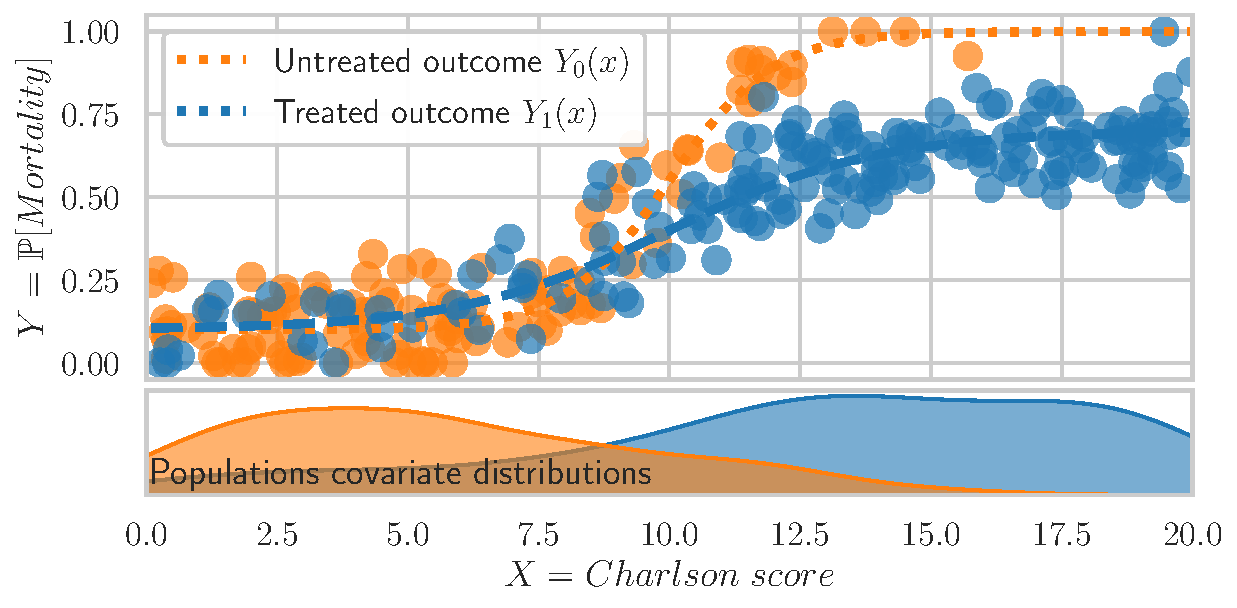
\includegraphics[width=1\linewidth]{img/chapter_1/sample.pdf}%
    \vfill%
    {\sffamily\footnotesize\scalebox{0.9}{b) Interventional data}}
    \vfill%
    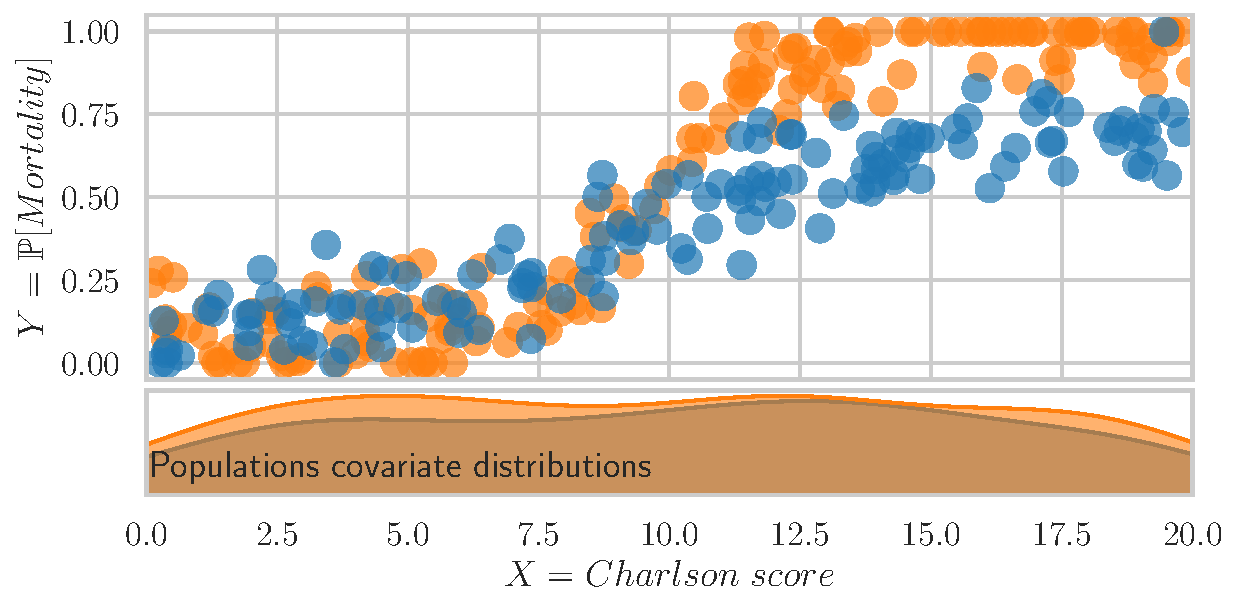
\includegraphics[width=1\linewidth]{img/chapter_1/sample_rct.pdf}%
  \end{minipage}
\end{figure}

\begin{background_box_left}

  % interventional  
  For interventional data --shown in Figure
  \ref{intro:fig:observational_vs_interventional}b), the randomization forces
  the probability of receiving the treatment for every patient --often to 50\%.
  Importantly, it is independent from patient characteristics such as the
  Charlson score. This favors the comparability between treated patients and
  control patients: Once this randomization has been repeated over many
  patients, \emph{on average}, the difference in outcomes can only be attributed
  to the treatment.

  % the distinction
  \cite{rothman2012epidemiology} distinguishes RCTs from observational data as
  follows: \textit{In an experiment, the reason for the exposure assignment is
    solely to suit the objectives of the study; if people receive their exposure
    assignment based on considerations other than the study protocol, it is not a
    true experiment.} Epidemiological textbooks highlight the experimental setup
  since randomization yields excellent \emph{internal validity}
  \citep{campbell1957factors}: The estimated average treatment effect is close to the
  true treatment effect if we could repeat the experience indefinitely on the
  same population --the average estimate is \emph{unbiased}. Statistical assumptions for
  the RCT methodology are easily met \citep[Section 3.1.1]{colnet2020causal} and involve the
  measurements of only two variables: the treatment and the outcome. This
  simplicity contributed to its success for clinical evidence generation.

  \paragraph{External validity: when RCTs insufficiently inform practices}\label{def:external_validity}
  % threat to external validity
  Interventional data are hard to collect: patients must be voluntary, without
  comorbidities, adhering to the treatment. These requirements contribute to
  idealized populations recruited in RCTs, endangering the \emph{external
    validity} of interventional studies
  \citep{feinstein1997problems,concato2000randomized,rothwell2005external}: The
  findings of a study may not generalize to other populations. As a practical
  consequence, RCTs may not apply to real world situations since included
  populations and experimental conditions differ too much from usual practices.
  For example, only 6\% of asthmatics would have been eligible for their own
  treatment RCTs \citep{travers2007external}. An advantage of observational data
  over RCTs is their description of usual care practices, opening a window on
  care effectiveness \citep{cochrane1972effectiveness}: How well does a
  treatment work in practice, outside the ideal circumstances of the
  experimentation ?

  % link with economics
  External validity have been raised in economics earlier than in epidemiology
  \citep{deaton2020randomization}. The focus in such problems is probably
  greater in economics because situations are not well controlled:
  economic agents act outside of the laboratory. On the contrary, clinical
  situations are closer to laboratory settings. This difference in data sources and
  methodology is visible in the divide between clinical and social epidemiology
  \citep{zielhuis2001social}. What about medico-economics ? I do not address this question in the
  present thesis, but it is a clear motivation.

  % Link with personalized medicine
  \paragraph{Heterogeneity of treatment: the link with personalized medicine.}

  % HTE and precision medicine
  The previous paragraph discussed average treatment effect. However,
  heterogeneity of treatment among subgroups is also an object of interest in
  healthcare \citep{hernan2020causal}. It is at the heart of the personalized
  medicine paradigm --also coined as precision medicine. Originally anchored into
  genomics, this concept tries to take individual variability into account for
  tailored treatment recommendations \citep{schork2015personalized,
    topol2019high}.

  % RL  
  In sequential decision making problems, heterogeneity of
  treatment effect is close to subfields of machine learning such
  as operational research \citep{schaefer2004modeling} or reinforcement learning
  \citep{bareinboim2015bandits}. These fields are focused on sequential
  decision making processes with a large action-state space, rather than one-off
  treatment as in this thesis. To robustly estimate the probabilities involved
  in large dimensional state-action spaces, these works often require a
  simulated environment \citep{bennett2013artificial}. Simulations allow to
  collect large samples of trajectory implementing the policy to be evaluated
  but are hard to build for complicated problems such as patient trajectories.
  Bridges with healthcare and personalized medicine include application in
  optimizing antiretroviral therapy in HIV \citep{guez2008adaptive} or
  management of sepsis in the Intense Care Unit \citep{komorowski2018artificial}
  but lack wide adoption \citep{senn2018statistical}.

\end{background_box_left}


\section{Two cultures of statistics for health}\label{sec:intro:two_cultures}

\cite{breiman2001statistical} clearly distinguished two statistical cultures: a
predominant community at the time focused on models, and an emerging trend that
rely only on predictive accuracy. The latter is now called machine learning.

\subsection{Model-based statistics: oracle domain experts}%
\label{subsec:intro:biostatistics_framework}

% focus of biostats and epidemiology on models
Biostatistics puts a strong emphasis on model specification, often interpreting
model parameters as valid nature constructs \citep{cox2001statistical}. Maybe because
epidemiology seek to estimate causes and effects, it also favors the model-based
culture as one can judge from textbooks \citep{rothman2012epidemiology}:
\textit{In many epidemiological applications, it is the choice among effect
  measures that dictates the type of model the investigator ought to use.} In
medical journals, Cox model for survival data and logistic regression for binary
outcomes have been the standard for publication. %
% why simple models ? because they are simpple
It is tempting to link explicit relations between variables in linear models to
claims over the data. But interpretability of the model parameters is a strong
assumption \citep{lipton2018mythos}, which relies on the well-specification of
the model: The underlying variables and their relations built into the models
should describe \emph{real} mechanisms.

% Importance of validity by generalization of theory rather than statistical
%   generalization: established epidemiological knowledge should \textit{tell us
%     what to expect in people or settings that were not studied.} Statistical
%   generalization is considered by \cite{rothman2012epidemiology} as applied
%   epidemiology, focused on specific cases and not as the core of epidemiological
%   science.


% choice of correct models and interpretability are strong assumptions
Despite judging model choice as \textit{crucial to fruitful application}
\citep{cox2006principles}, this tedious task is left to experts, that should have an
appropriate theoretical model of the problem \citep{cox2001statistical}. This
habit is prone to circular reasoning where a model is chosen only to justify an
established theory. Crowdsourcing studies asking the same question to
different teams of experts showed that the choice of model and features is far
from consensual and yield substantially different quantitative and qualitative
results. \cite{botvinik2020variability} attributed this dispersion to different
modeling choice in a crowdsourced analysis of brain imaging data by 70 teams.
\cite{schweinsberg2021same} showed that theoretical constructs --how the
model input variables are defined from raw data-- also contribute to the heterogeneity of results.
All of these studies followed the model-based culture, assuming specific linear
models and interpreting their inner part as causal.

% Note that other domain of science, such as particle physics departed from
% elaborated models. Recent studies on the Higgs bosons use flexible machine
% learning models as a mean for parameter identifications, without attributing a
% particular sense to their inner working \citep{varoquaux2021ai}.

\begin{background_box_left}

  \subsection{Machine learning: black-box predictive ability?}\label{subsec:intro:machine_learning}

  Departing from carefully designed functional forms for statistical models,
  algorithms emerged in the late 90s to automatically learn patterns in the
  growing body of complex data. Among them, one can cite random forests,
  gradient boosting, neural networks or support vector machines.

  \paragraph{Supervised learning}

  Statistical learning \citep{vapnik1999nature} is the theoretical framework
  underpinning machine learning. It has been introduced in the 1960s and
  popularized in the 1990s with the developments of flexible pattern recognition
  models. It is concerned with empirical risk minimization: Finding good
  approximation of the features-outcome association. Appendix
  \ref{apd:intro:statistical_learning} recalls the formal definition of the
  supervised regression problem. Appendix \ref{apd:intro:statistical_models}
  details the principles of random forest and gradient boosting since we are
  using these two algorithms in different chapters of this thesis.

  \paragraph{Model selection: how to choose between multiple promising models}

  Choosing the best model among a family of potential estimators is done by
  comparing their performances on an unseen test dataset. If we were to evaluate
  a model on the same data that it has been trained on, we would systematically
  favor flexible models that adapt better to the sampled training data. To avoid
  this process called \emph{overfitting}, the analyst should separate the data
  on which an estimator is fitted --the training set-- from the data used to
  chose the estimators --the test set. To avoid data loss, cross-validation
  \citep{stone1974cross} proceeds in multiple rounds of training and testing on
  the same data as illustrated in Figure \ref{fig:intro:cross_validation}. The
  data is divided in K folds --typically 5 to 10--. Then, each fold is part of
  the training set K-1 time and is used once as test set. Algorithms are then
  selected on the average performances over the K test sets.

  Note, that despite being valid for model selection --choosing the best model,
  cross-validation yields biased estimates to evaluate a given model
  \citep{wager2020cross}. Nested cross-validation has been proposed as a simple
  way to perform this final model evaluation \citep{varoquaux2017assessing}.

\end{background_box_left}

\begin{figure}[!b]
  \centering
  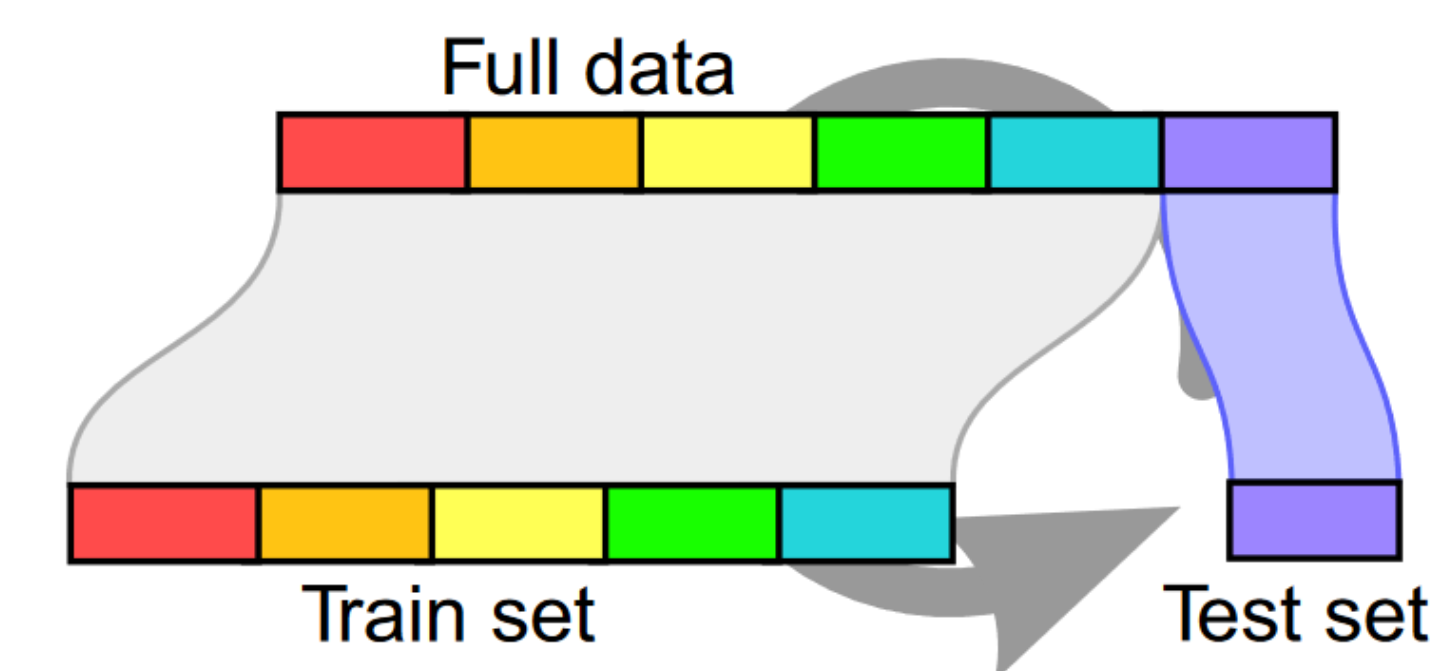
\includegraphics[width=0.8\linewidth]{img/chapter_1/cross_validation.png}
  \caption{Cross-validation: the data is split into training and testing sets.
    The training set is used to fit the model. The testing set is used to
    evaluate the model. The process is repeated multiple times to avoid
    overfitting. Original figure from \cite{varoquaux2017assessing}.}
  \label{fig:intro:cross_validation}
\end{figure}

\begin{background_box_left}

  \paragraph{Pre-training: from learning patterns to learning representations}
  % what is it
  As of 2012, the success of deep neural networks in computer vision
  \citep{krizhevsky2012imagenet}, sparkled interest for representation learning.
  Grounded in information theory, this subfield of machine learning is concerned
  in automatically building low dimensional features from raw data that capture
  \emph{useful information} \citep{bengio2013representation}. A good
  representation should keep information on the output $y$ and loose non-useful
  information in the input $x$, making it robust to noise: I refer to
  \cite{achille2018emergence} for a detailed formalization. This definition of
  usefulness highlights the need to find pretext tasks to supervise the learning
  of representations. For example, in computer vision, the pretext task is to
  label coarse classes of images (eg. dog, cat, container, ...). In NLP, the
  pretext task is to predict randomly masked world in a text. These tasks should
  be weakly-supervised in the sense that they do not require human annotations.
  The learned representations are then used as input to a supervised task, which
  should be close enough from the pretext task to leverage information retained
  during pre-training.

  % Why am I not doing this
  This thesis was originally motivated by studying deep representations for
  patient trajectories and their ability to transfer between healthcare
  databases. However, I progressively realized that the choice of a
  representation loops back to the choice of a model, and hence to the measure
  of performances for relevant downstream tasks. For other domains such as NLP,
  consensual downstream tasks such as text classification have been established
  to evaluate the performances of representations. Aggregated in benchmarks such
  as GLUE \citep{wang2018glue}, these tasks fueled model developments for years.
  Recently, \cite{raji2021ai} pointed out the risk of misalignment between
  machine learning benchmarks and research claims about a task or real world
  objectives --what they call construct validity. This criticism is also pertinent
  for RWD since interests in using these data are fragmented --as developed in
  the next section. Moreover, healthcare interest in pure predictive problems is
  unclear --see Section \ref{sec:causal_tuto:motivation}. Finally, the
  circulation of data or representations in healthcare are almost non-existent
  for confidentiality purposes. These specific features of RWD call into
  question the appropriateness of constructing universal representations in
  healthcare.
  % Focus on variable selection: root in hand collected variables in carefully
  % designed subpopulation ?

  % Focus on simple models for juridical and credibility reasons but also for
  % practical reasons: the input data should be readily available to question one
  % model individual prediction \citep{wyatt1995commentary}.

  % \textit{Often the prediction is under quite different conditions from the
  % data; [...] what would be the effect on annual incidence of cancer in the
  % United States of reducing by 10\% the medical use of X-rays}. This example is
  % a pure causal inference question.

\end{background_box_left}


% Focus of the thesis
\subsection{One choice of perspective: Recent statistical learning for EHRs}%
\label{subsec:intro:focus_data}%

% EHR is highly dimensional (at least with temporality and high cardinality of categorical features)
In this thesis, we focus on EHRs, even if some of our results could be relevant
for insurance claims as well. The complexity of using EHRs in statistical
frameworks is linked with their potential to address complex questions in public
health: they register almost all aspect of the hospital care trajectories.
Therefore, the dimensionality of EHRs data is high: diagnoses, laboratory
measurements and procedures are logged with medical terminologies having ten of
thousands of codes; unstructured text data is by nature high dimensional.
Finally, the temporal dimension of EHRs poses a challenge for statistical
models, usually assuming a static vector of features for each unit.
% This perspective reflects the modern tendency to go to more elaborated models
% and richer data.
For such high dimensional data where the number of (selected) features could
easily reach the hundreds, linear models are not strictly more interpretable
than deep neural network \citep{lipton2018mythos}. Therefore, it is tempting to
turn towards machine learning techniques to leverage the full potential of EHRs.
% 
% \paragraph{This perspective reflects more naturally my progression:} Learning
% statistics in the age of deep learning pushes towards adopting a view on
% statistics that consider mechanisms as generally unknown, and predictive
% accuracy as the hallmark of validity \citep{breiman2001statistical}.
Are flexible statistical models a valid tool to answer today's questions in
healthcare? If we are concerned in identifying which levers to pull to improve
healthcare, we might not need to specify in our statistical models all
mechanisms involved in the care process and its interaction with the complex EHR
measurement system. One can hope that sufficient amount of data would allow flexible algorithm to
detect useful regularities in the data and learn from them
\citep{halevy2009unreasonable}.

% A practical stance balances
% between good predictive performances --low error rates-- and adoption by
% practitioners. The latter built upon trust, an aspect of interpretability that
% increases when estimator error cases are the same as human errors
% \citep{lipton2018mythos}.


\section{Important questions in public health}%
\label{sec:intro:causality}%

\subsection{The promises of RWD: what pressing needs to use health data}

The recent increase in RWD collection is attracting the attention of many
players. The optimism on the promises of healthcare data is shared by
epidemiologists \citep{mooney2015epidemiology,hernan_using_2016}, AIM researchers
\citep{schwartz1987artificial, yu2018artificial}, clinical researchers
\citep{schwalbe2020artificial,dzau2023anticipating}, the industry
\citep{pfizer2019rwd,iqvia2023rwd} and government bodies
\citep{mcginnis2013best,fda_real_2018,ema2023rwd}. New scientific journals such
as the \emph{NEJM AI}\footnote{\url{https://ai.nejm.org/}} \citep{beam_2023} at
the intersection between algorithmic advances and clinical practices
demonstrate the sustained interest in leveraging RWD for improving healthcare.

Drawing a full picture of these expectations would be over-ambitious and
partial. But I think it is relevant to disentangle them in order to delimitate
clearly the scope of questions that motivate my work. As discussed in Section
\ref{sec:intro:landscape}, these motivations stem from a machine learning
formation and public health concerns.

%primary use
\paragraph{Primary uses of health data focus on patient care.}

EHRs are primarily used to record patients' health state and cares
\citep{safran_toward_2007,eu_primary_2022}. This information might be shared
within the healthcare team, but always with the goal to cary for the patient
whose data is collected. Direct benefits to the patients are provided thanks to
more detailed and searchable information than paper-based medical records. These
benefits are amplified in modern care systems where patient trajectories are
fragmented between numerous healthcare professionals.

% A recent work on the classification of data and models (AI) in clinical medicine
% suggests three main usages: AI in clinical practice, clinical research on AI/ML
% device and applications and AI/ML used to conduct clinical research
% \citep{haug2023artificial}.

\paragraph{From the automation of the care workflow to personalized medicine.}

% AI in healthcare 
The automation of tedious tasks in healthcare is part of the original agenda of
AIM \citep{schwartz1987artificial}. The goal is to give more time to the
physicians by accelerating and facilitating parts of their work that require
poor analytical capacities.
% Old example of such automation is the computer reading of electrocardiograms. A
% recent example is the assistance of Large Language Model such as GPT-4 for
% medical note taking \citep{lee2023benefits}. 
%However, the incentives to collect and analyze data
% vary among the different healthcare actors.
% The first works on Artificial Intelligence in Medicine (AIM) dates back to the
% early 70s and was focused on diagnostic, computer-aided decision making and
% automated consultations \citep{shortliffe1976computer}.  

Recent discourse and successes are heavily influenced by this line of though,
with the aim to automate ever more specialized parts of care. Machines read
medical images faster and more efficiently than most practitioners
\citep{zhou2021review}. Structured data from Electronic Health Records
\citep{rajkomar2018scalable} or administrative databases
\citep{beaulieu2021machine} outperform rule-based clinical scores in predicting
patient's readmission, in-hospital mortality or future comorbidities
\citep{li2020behrt}. Recently, large language models (LLMs) leveraged clinical
notes from several hospitals for length of stay prediction
\citep{jiang2023health}. Hope is high that LLMs models will soon be able to help
practitioners during consultation \citep{lee2023benefits}. The trend towards
personalized medicine is gradually moving away from the automation of
well-understood but tedious tasks to tailored individual care, where mechanisms are less
understood \citep{schork2015personalized, topol2019high}.

\paragraph{New data for better knowledge acquisition?}

%Better understand what and why think works
RWD data also bring indirect benefits --secondary uses-- by accelerating and
improving knowledge production: on pathologies
\citep{campbell_characterizing_2022}, on the conditions of use of health
products and technologies \citep{safran_toward_2007,tuppin_value_2017}, on the
measures of their safety \citep{wisniewski_development_2003}. They can also be
used to assess the organizational impact of health products and technologies
\citep{has_guide_2020,has_real-world_2021}. These descriptive usages are closer
to the main goal of epidemiology: \textit{the study of the distribution
  and determinants of disease frequency} \citep{macmahon1970epidemiology}.

% Monitoring and evaluation: public policy and industry, two faces of the same coin
Health Technology Assessment (HTA) agencies in many countries have conducted
extensive work to better support the generation and use of real-life data
\citep{fda_real-world_2021,has_real-world_2021,kent_nice_2022,plamondongenevieve_integration_2022}.
Study programs have been launched by regulatory agencies: the DARWIN EU program
by the European Medicines Agency and the Real World Evidence Program by the Food
and Drug Administration \citep{fda_real_2018}. However, recent surges in data
collection also encouraged deviation from the standard interventional design by
relaxing some of the methodological constraint of RCTs. HTA agencies witnessed a
deterioration of evidences for new drugs and strongly advocate against
observational studies for replacing new drugs evaluation
\citep{wieseler2023replacing,vanier2023rapid}. This debate crystallizes tensions
between the pharmaceutical industry and regulators since drug prices are
mainly driven by drug efficacy (assessed in trials).
%
There is still active debates to better understand what is the place of these
data to develop new evidence on the effectiveness of interventions --see
\ref{def:external_validity} \citep{richesson_electronic_2013,wang2023emulation}.
%\md{develop: schneeweiss and the replicate program}.
% % too much
% Industries also have a strong interest in gathering and analyzing data. For
% market access, they need to carefully describe what population is reached by
% their product.

\paragraph{Public health questions: old and new}

The \emph{Coming revolution In Medicine} is described by
\cite{rutstein1967coming} as:\textit{1) modern medicine's skyrocketing costs; 2)
  the chaos of an information explosion involving both paperwork proliferation and
  large amounts of new knowledge that no single physician could hope to digest; 3)
  a geographic maldistribution of M[edical] D[octors]s; 4) increasing demands on
  the physician's time as increasing numbers of individuals began to demand
  quality medical care.} Fifty years later, the same preoccupations are
destabilizing healthcare systems in rich countries: increasing costs
\citep{data_oecd_health_spending}, knowledge produced too quickly to be
assimilable by a single person \citep{mcginnis2013best}, geographic disparities
and lack of trained physicians \citep{anguis2021quelle,aamc2021}.

In this context, public health authorities are asked to better understand what
cares are the most effective. With constrained medical resources, efforts should
be focused on the most effective interventions and prevent unnecessary cares.
However, measuring the appropriateness of a care is a delicate question
\citep{cma_policy_appropriateness_2015}. Scientific associations and regulators
issue medical guidelines built upon the scientific literature to recommend ideal
care trajectories. However, these recommendations often focus on single-disease
approaches, insufficiently covering today's population of patients: increasingly
old and multimorbid \citep{skou2022multimorbidity}. Fewer than half of the
clinical guidelines for the nine most common chronic conditions consider older
patients with multiple comorbid chronic conditions
\citep{boyd2005clinical,parekh2010challenge}. In the United States, the
Committee on Learning Healthcare System suggested to better use routine data to
adapt evidence to real practice and accelerate its diffusion
\citep{mcginnis2013best}.

In line with this roadmap, this thesis is motivated by the opportunities offered by
EHRs to evaluate the effectiveness of medical guidelines. Formally, a
guideline can be expressed as an action (or a series of actions) to take given a
patient risk profile. The action/characteristic reflects the
practice of  physicians: they see and listen to a patient, then take
appropriate actions given its profile. A medical recommendation tries to
guide this link between patient characteristics and intervention.

\begin{background_box_left}

  \subsection{Prediction or causation?}%
  \label{subsec:intro:prediction_causation}%

  % Can I use plain prediction for this question?
  Is statistical learning a useful tool to answer these questions? There is a
  growing interest in predictive models in healthcare. This trend is reflected
  by the exponential increase in the proportion of publications per year in
  Pubmed shown in Figure \ref{fig:intro:pubmed_query}. However, when reading
  into details the prognosis literature I was surprised to find that prediction
  is rarely an objective per-se.

  % Epidemiological books, confounding is the very first explained concept
  % \citep{rothman2012epidemiology}.
  % Causes are mainly presented as binary variables absent or present in
  % epidemiology textbooks \cite{rothman2012epidemiology}. Their strength is only
  % defined at a population level, making them relative to a given population
  % \citep[chapter~3]{rothman2012epidemiology}. This point of view is rather
  % aligned with statistical modeling related to variable significance, not with
  % model performances.
  % Interesting concept of promoter, the last component cause that precede the
  % apparition of a disease.
  % AIM is rooted in causality 
  The early Framingham study concludes that risk reduction is more important
  than identifying the strength of specific risk factors since this quantity is
  subject to slight changes in the risk model \citep{brand1976multivariate}:
  \textit{It further suggests that the strength of a particular risk factor may
    not be as important from the point of view of intervention as the ability to
    safely and conveniently achieve even a moderate risk reduction in a large
    number of persons.} In a foundational article on EHR, heart failure prediction
  is motivated by aggressive interventions \citep{wu2010prediction}:
  \textit{heart failure could potentially lead to improved outcomes through
    aggressive intervention, such as treatment with angiotensin converting enzyme
    (ACE)-inhibitors or Angiotensin II receptor blockers (ARBs)}. More recently,
  \cite{beam2018big} devise a machine learning spectrum, making the distinction
  between algorithms requiring heavy human assumptions and flexible models. But
  the goal of these algorithms is almost always to serve
  \textit{decision-making}, not prediction. It is clearly described by
  \cite{steyerberg2009applications} for diagnosis: \textit{If we do a diagnostic
    test, we may detect an underlying disease. But some diseases are not
    treatable, or the natural course might be very similar to what is achieved
    with treatment.} Modeling has always been judged necessary but it is only
  recently that pattern recognitions is pursued as an objective per-se,
  associated with an exponential disinterest for causality as shown in Figure
  \ref{fig:intro:pubmed_query}. \cite{patel2009coming} discussed the
  inappropriateness of the unsupervised and supervised approaches: They
  \textit{tend to discover relatively simple relationships in data and have not
    yet demonstrated the ability to discover complex causal chains of
    relationships.} This make them misaligned with scientific and practical
  objectives which are to \textit{formulate and test hypotheses about how the
    human organism “works” in health and illness}.

  The auxiliary role of prediction in healthcare calls for replacing or
  complementing statistical learning with another methodological tool.


\end{background_box_left}

\begin{figure}
  \centering
  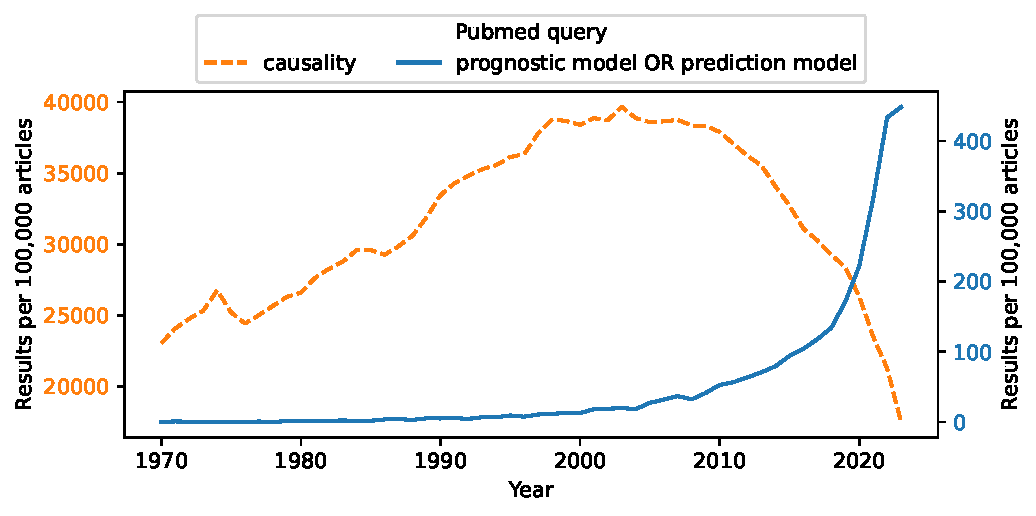
\includegraphics[width=0.8\textwidth]{img/chapter_1/pubmed_query.pdf}
  \caption{Proportion of articles by year in Pubmed returned by queries on
    causality (orange) or predictive modeling (blue). The scale differs greatly
    but the symmetry of the trends is disturbing.}%
  \label{fig:intro:pubmed_query}
\end{figure}

\begin{background_box_left}

  % Figure \ref{fig:intro:pubmed_query} illustrate this tension between prediction
  % and causation. It represents the proportion of articles per year in Pubmed
  % mentioning predictive modeling as in \cite[Chapter
  %   1]{steyerberg2009applications} and contrast this exponential upward trend with
  % the downward trend in causality.


  \paragraph{The central concept of causality}%
  \label{subsec:intro:causation}%

  Causality is an central concept in epidemiology
  \citep{hill1965environment,hernan2020causal} and have been developed formally
  in statistics \citep{rubin1974estimating}, econometrics
  \citep{imbens2009recent} and machine learning \citep{pearl2018book}.

  % causality in ML
  Causality departs from classical statistics by stressing the importance of
  interventions: the strong correlation between an outcome and a feature is no
  evidence of a causal link between them. This central point has been depicted
  as the ladder of causation \citep{pearl2018book}: For a given set of
  observations, multiple consistent causal models exist, only one of which
  correctly reflects the reality. For concreteness, I transcribe the didactic
  example from \cite{murphy2022probabilistic_chapter36}: \textit{Consider three
    possible explanations for the association between ice cream and drowning.
    Perhaps eating ice cream does cause people to drown—due to stomach cramps or
    similar. Or, perhaps, drownings increase demand for ice cream—the survivors
    eat huge quantities of ice cream to handle their grief. Or, the association
    may be due (at least in part) to a common cause: warm weather makes people
    more likely to eat ice cream and more likely to go swimming (and, hence, to
    drown). Under all three scenarios, we can observe exactly the same data, but
    the implications for an ice cream ban are very different. Hence, answering
    questions about what will happen under an intervention requires us to
    incorporate some causal knowledge of the world—e.g., which of these scenarios
    is plausible?}\md{Find better than this ice cream example?}

  % Connexion with important questions in healthcare: 
  Causality also has connections with other important issues in healthcare such
  as fairness \citep{plecko2022causal} or dataset shift, linked to the representativity of a
  dataset \citep{subbaswamy2020development}. We did not explore these aspects,
  but they motivate part of the work in Chapter \ref{chapter:causal_tuto}.

  \paragraph{A robust statistical framework: Neyman-rubin}%
  \label{subsec:intro:causal_framework}%

  I recall the framework of the potential outcomes, which enables statistical
  reasoning on causal treatment effects \citep{imbens_causal_2015}. I will
  progressively introduce supplementary concepts as needed in Chapters
  \ref{chapter:causal_tuto} and \ref{chapter:causal_model_selection}.

  Given an outcome $Y \in \mathbb R$ (eg. mortality risk or hospitalization
  length), function of a binary treatment $A \in \mathcal{A} = \{0, 1\}$ (eg.~a
  medical procedure, a drug administration), and baseline covariates $X \in
    \mathcal{X} \subset \mathbb{R}^d$, we observe the factual distribution, $O =
    (Y(A), X, A) \sim \mathcal D = \mathbb P(y, x, a)$. However, we want to model
  the existence of potential observations (unobserved ie. counterfactual) that
  correspond to a different treatment. Thus we want quantities on the
  counterfactual distribution $O^{*} = (Y(1), Y(0), X, A) \sim \mathcal D^{*} =
    \mathbb P(y(1), y(0), x, a)$.

  Popular quantities of interest --estimands-- are: at the population level, the
  Average Treatment Effect
  \begin{flalign*}\label{def:ate}
    \text{ATE} &  &
    \tau \myeq \; \mathbb{E}_{Y(1),Y(0) \sim \mathcal D^*}[Y(1) - Y(0)];
               &  &
  \end{flalign*}
  %
  at the individual level, to model heterogeneity, the Conditional Average Treatment Effect
  \begin{flalign*}
    \text{CATE} &  &
    \tau (x) \myeq \; \mathbb{E}_{Y(1),Y(0) \sim \mathcal{D}^\star}[Y(1) - Y(0) | X=x].
                &  &
  \end{flalign*}

  We might be tempted to equate the mean of a potential outcome to the mean of
  the observed outcome conditionally on the treatment. However, in general:
  $\mathbb E[Y(a)] \neq \mathbb E [Y|A=a]$. This is because the right hand side
  reads as \emph{the expected value of Y given A =a}, thus we restrict the
  outcome to the individuals that actually received the treatment. If this group
  has different outcomes than the other group, the equality does not hold as
  illustrated in Figure \ref{intro:fig:observational_vs_interventional}.

  The statistical assumptions required to estimate these quantities from
  observational data are presented in Section
  \ref{subsec:causal_tuto:identification}. The common methods used for the
  estimations are detailed in Appendix \ref{apd:causal_estimators}.

\end{background_box_left}

\section{Contributions}\label{sec:intro:contributions}

% In the 2000s, the AIM themes were listed as \textit{knowledge representation and
%   ontology development, terminology and semantic modeling of domains, decision
%   support and reasoning under uncertainty, model-based image processing}
% \citep{patel2009coming}.
% Edward H. Shortliffe insisted on the shift from individual patient specific
% decision-support to guideline-based decision support, a movement that also took
% place in clinical medicine. In the same paper, Mario Stefanelli insists on the
% importance of Knowledge Management which goal \textit{is to improve
%   organizational performance by enabling individuals to capture, share and apply
%   their collective knowledge to make optimal "decisions in real time"}.
% When listing the four future needs of the AIM community, Szolovitz first
% mentioned data collection, then improved design for workflow, better reassuring
% techniques for data privacy and lastly better modeling techniques. Workflow
% benefits should outweigh the distribution they create. Many medical errors are
% due to omission rather than commission, suggesting the need for continuous
% monitoring systems.

% objective
First influenced by the growing successes of machine learning in predictive
modeling, this thesis seeks to understand what models and framework might help
evaluating the effectiveness of clinical guidelines using the time varying and
high dimensional Electronic Health Records. What predictive models are useful ?
Why prediction is not enough ? How flexible models can serve the true
objective of healthcare: delivering appropriate treatment to each and every
patient to improve her health \citep{cma_policy_appropriateness_2015}?

The contributions of each chapter, which are summarized below, have led to three
articles as first-authors and one work in progress:

\begin{itemize}
  \item Chapter \ref{chapter:cdw} published in \emph{PLOS Digital Health},
  \item Chapter \ref{chapter:predictive_models} is ongoing work,
  \item Chapter \ref{chapter:causal_tuto} submitted to \emph{npj Digital Medicine},
  \item Chapter \ref{chapter:causal_model_selection} submitted to \emph{Artificial Intelligence in Medicine}.
\end{itemize}

Beyond these works, applied projects have also been conducted, leading to one
other research work linked to invasive ICU treatment disparities, co-authored
with Sara Mohammed, João Matos, Leo Anthony Celi and Tristan Struja. This work
has been accepted to \emph{Yale Journal of Biology and Medicine} (third-position
author). On this project I helped on the design of the statistical analysis,
more particularly on the model selection procedure with machine learning
algorithms.

This work is a specific application separated from the thesis main questions.
Therefore it is not detailed in this manuscript.

\md{Justify the chapters and link them}
\paragraph{Chapter \ref{chapter:cdw}: Potential and challenges of Clinical Data
  Warehouse, a case study in France} This chapter draws the first overview of
  the Clinical Data Warehouses (CDWs) in France. These technical and
  organizational infrastructures are emerging in the hospitals to collect and
  analyze the data produced in Electronic Health Records. This work is an
  attempt to better characterize the reality of data reuses in university
  hospitals. It documents key aspects of the collection and organization of
  routine care data into homogeneous databases: governance, transparency, types
  of data, data reuse main objectives, technical tools, documentation and data
  quality control processes. The qualitative aspect of this chapter contrasts
  with the general mathematical context of the thesis.

\paragraph{Chapter \ref{chapter:predictive_models}: Exploring a complexity
  gradient in representation and predictive algorithms for EHRs} Acknowledging
  the growing interest in predictive algorithms for EHR data, this chapter
  introduces two simple feature construction methods taking raw medical events
  as input features. It benchmarks four predictive pipelines of increasing
  complexity on three predictive tasks: length of stay interpolation, next visit
  prognosis and cardiovascular adverse events prediction. It focuses on medium
  sized datasets where the population at risk (after inclusion rules) ranges
  from 10,000 to 20,000 samples. In these setups, this work explores the
  complexity-performance tradeoff from simple baseline models to recent
  transformer-based neural networks. 

\paragraph{Chapter \ref{chapter:causal_tuto}: Prediction is not all we need:
  Causal thinking for decision making on EHRs}


\paragraph{Chapter \ref{chapter:causal_model_selection}: How to select
  predictive models for causal inference?}

\chapter{Potential and challenges of Clinical Data Warehouse, a case study in France}%
\label{chapter:cdw}%


\begin{citationbox}
  Souvent, entre [la construction des données et leur traitement ou leur
      interprétation], se dresse la "banque de données", qui fonctionne comme un
  sas de passage de l'une à l'autre. Or le monde de la "construction" est
  lui-même tendu entre deux façons de rendre compte de ses pratiques : la
  mesure, issue du langage des sciences de la nature, le codage conventionnel,
  inspiré, selon les cas, du droit, des sciences politiques, ou des sciences
  cognitives.%
  \par\hfill -- Alain Desrosière, \textit{Entre réalisme métrologique et
    conventions d'équivalence : les ambiguïtés de la sociologie quantitative}
\end{citationbox}

\vspace{2cm}

\begin{chapterabstract}\label{sec:cdw:abstract}%
  Despite increasing collection of routine care data, reusing it does not come
  free of charges. Attention must be paid to the entire life cycle of the data
  to create robust knowledge and develop innovation. In this chapter, we build
  upon the first overview of Clinical Data Warehouses (CDWs) in France to
  document key aspects of the collection and organization of routine care data
  into homogeneous databases: governance, transparency, types of data, data
  reuse main objectives, technical tools, documentation and data quality control
  processes. The landscape of CDWs in France dates from 2011 and accelerated in
  the late 2020, showing a progressive but still incomplete homogenization.
  National and European projects are emerging, supporting local initiatives in
  standardization, methodological work and tooling. From this sample of CDWs, we
  draw general recommendations aimed at consolidating the potential of routine
  care data to improve healthcare. Particular attention must be paid to the
  sustainability of the warehouse teams and to the multi-level governance. The
  transparency of the data transformation tools and studies must improve to
  allow successful multi-centric data reuses as well as innovations for the
  patient. The qualitative aspect of this chapter contrasts with the general
  mathematical context of the thesis. We have borrowed the methodology from the
  field of sociology on the advice of Professor Emmanuel Didier.
\end{chapterabstract}


\vfill
\begin{flushright}
  \begin{minipage}{15cm}
    {\small{This chapter corresponds to the article entitled \textit{Good practices for clinical data warehouse
          implementation: A case study in France}
        \underline{published} to \textit{PLOS Digital Health},}}\\
    {\small\hfill{} Authors: Matthieu Doutreligne, Adeline \textsc{Degremont}, Pierre-Alain
    \textsc{Jachiet}, Antoine \textsc{Lamer} and Xavier \textsc{Tannier}.}
  \end{minipage}
\end{flushright}


\clearpage
\minitoc

\section{Motivation and background: A changing world}\label{sec:cdw:motivation}

\begin{background_box_left}

  \subsection{Healthcare data collection is tightly linked with local organization}%
  \label{subec:cdw:local_organization}%

  In practice, the possibility of mobilizing routinely collected data depends on
  their degree of concentration, in a gradient that goes from centralization in
  a single, homogenous Hospital Information Systems (HISs, \ref{def:ehr_his}) to
  fragmentation in a multitude of HIS with heterogeneous formats. The structure
  of the HIS reflects the governance structure. Thus, the ease of working with
  these data depends heavily on the organization of the healthcare actors.

  \paragraph{Claims data are often centralized by national agencies}

  In South Korea, the government agency responsible for healthcare system
  performance and quality (HIRA) is connected to the HIS of all healthcare
  stakeholders. HIRA data consists of national insurance claims
  \citep{kyoung2022understanding}. England has a centralized health care system
  under the National Health Service (NHS). Despite, not having detailed clinical
  data, this allowed the NHS to merge claims data with detailed data from two
  large urban medicine databases, corresponding to the two major software
  publishers \citep{opensafely_system_one_data_2023}. This data is currently
  accessed through Opensafely, a first platform focused on Covid-19 research
  \citep{opensafely_2022}. In the United States, even if scattered between
  different insurance providers, claims are pooled into large databases such as
  Medicare, Medicaid or IBM MarketScan. Lastly, in Germany, the distinct federal
  claims have been centralized only very recently \citep{kreis2016status}.

  \paragraph{Clinical data are mostly distributed among many entities}

  Despite different interoperability choices, large institutional clinical
  data-sharing networks begin to emerge. South Korea very recently launched an
  initiative to build a national wide data network focused on intensive care.
  United States is building Chorus4ai, an analysis platform pooling data from 14
  university hospitals \citep{chorus4ai_2023}. To unlock the potential of clinical
  data, the German Medical Informatics Initiative \citep{gehring_german_2018}
  created four consortia in 2018. They aim at developing technical and
  organizational solutions to improve the consistency of clinical data.

  Israel stands out as one of the rare countries that pooled together both claims
  and clinical data at a large scale: half of the population depends on one single
  healthcare provider and insurer \citep{clalit_data_2023}.

  \paragraph{The case of France}

  In France, the national insurer collects all hospital activity and city care
  claims into a unique reimbursement database \citep{tuppin_value_2017}. However,
  clinical data is historically scattered at each care site in numerous HISs.

\end{background_box_left}


\subsection{An infrastructure fo healthcare data : The Clinical Data
  Warehouses}%
\label{subsec:cdw:cdw_definition}%

\paragraph{Dedicated infrastructures, called Clinical Data Warehouse (CDW)} are
needed to pool data data from one or more medical information systems --whatever
the organizational framework-- to homogeneous formats, for management, research
or care reuses \citep{chute_enterprise_2010,pavlenko_implementation_2020}. Fig
\ref{background:CDW:fig:ehr_flow} illustrates for a CDW, the four phases of data
flow from the various sources that make up the HIS.

\begin{enumerate}
  \item \textbf{Collection} and copying of original sources.
  \item \textbf{Transformation}: Integration and harmonization
        \begin{itemize}
          \item Integration of sources into a unique database.
          \item Deduplication of identifiers.
          \item Standardization: A unique data model, independent of the
                software models harmonizes the different sources in a common schema,
                possibly with common nomenclatures.
          \item Pseudonymization: Removal of directly identifying elements.
        \end{itemize}
  \item \textbf{Provision} of sub-population data sets and transformed datamarts
        for primary and secondary reuse.
  \item \textbf{Usages} thanks to dedicated applications and tools accessing the
        datamarts and data sets.
\end{enumerate}


\begin{figure*}
  \centering
  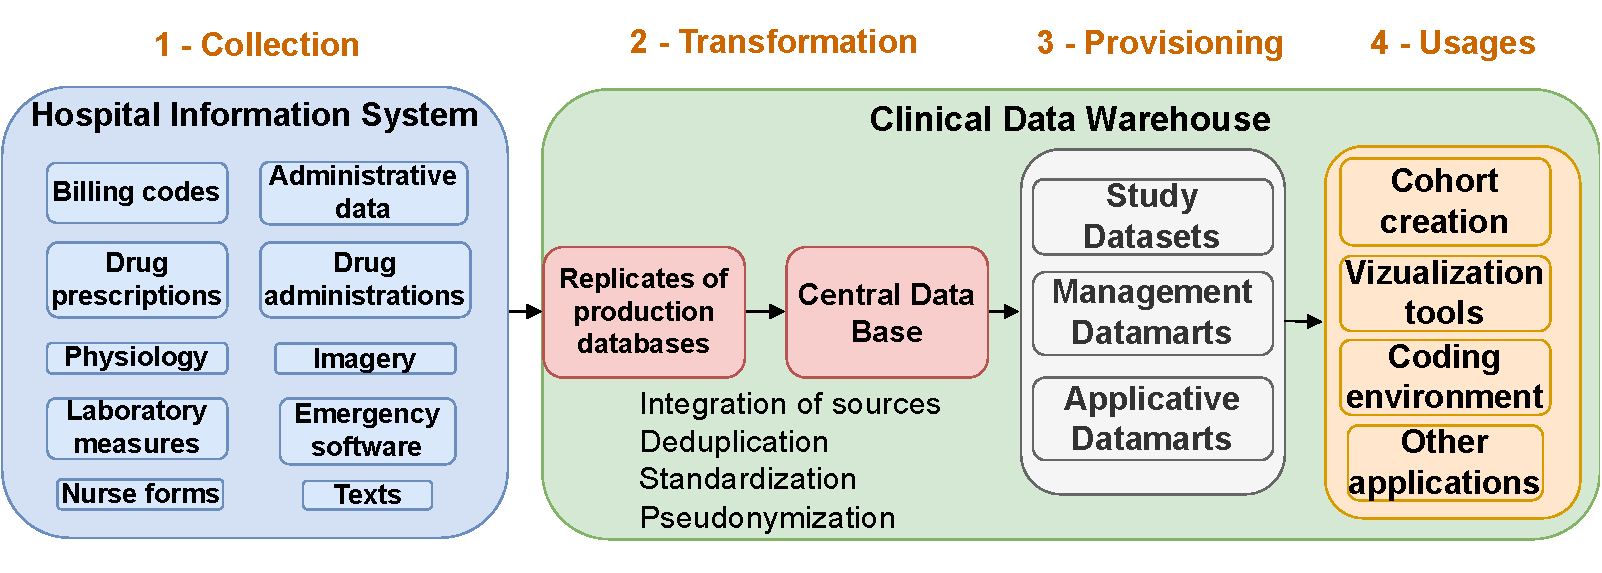
\includegraphics[width=1\linewidth]{img/chapter_2/Fig1.pdf}
  \caption{Clinical Data Warehouse: Four steps of data flow from the Hospital Information System: 1) collection, 2) transformations and 3) provisioning.}
  \label{background:CDW:fig:ehr_flow}
\end{figure*}


\paragraph{Multiplication of CDW in France} For about ten years, several
hospitals developed CDWs from electronic medical records
\citep{cuggia_roogle_2011,jannot_georges_2017,garcelon_finding_2017,wack_installation_2017,daniel_initializing_2018,malafaye_mise_2018,artemova_predimed_2019,lelong_building_2019,conan_les_2021,
  lamer_development_2022}. This work has accelerated recently, with the growing
development of dedicated infrastructures at the regional and national levels.
Regional cooperation networks are being set up --such as the Ouest Data Hub
\citep{hugo_2022}. In July 2022, the Ministry of Health opened a 50 million
euros call for projects to set up and strengthen a network of hospital Clinical
Data Warehouses (CDWs) coordinated with the national platform, the Health Data
Hub by 2025.

\paragraph{Poor understanding of CDW scope} Despite these few examples, the
precise scope of CDWs is still poorly understood: How are they created ? What
data do they process ? How common are they ? What studies do they run ?
Acknowledging the key importance of better structuring healthcare data, we
create the first overview of CDWs in France. We build upon this landscape, to
draw general recommendations aiming at consolidating the potential of routine
care data reuse.

\section{Speaking to the data collectors: Interviews of French University
  Hospitals}%
\label{sec:cdw:methods}%

Based on an overview of university hospital CDWs in France, this study make
general recommendations for properly leveraging the potential of CDWs to improve
healthcare. It focuses on: governance, transparency, types of
data, data reuse, technical tools, documentation and data quality control
processes.

Interviews were conducted from March to November 2022 with 32 French regional
and university hospitals, both with existing and prospective CDWs.

\subsection{Interviews and study coverage}\label{subsec:cdw:interviews}

\paragraph{Semi-structured interviews}

We conducted semi-structured interviews on the following themes: the initiation
and construction of the CDWs; the current status of the project and the studies
carried out; opportunities and obstacles; quality criteria for observational
research. S1 Table list all interviewed people with their team title.

We designed an interview form, sent to participants in advance. We used it as a
support to conduct 90 minutes interviews recorded for reference (the complete
form is available in Appendix \ref{apd:cdw:interview_form}).

Based on these interviews, we collected structured information on both the
characteristics of the actors, and those of the data warehouses. We completed
them based on the notes taken during the interviews, the recordings, and by
asking the participants for additional information. Detailed tables are
available on \url{https://gitlab.has-sante.fr/has-sante/public/rapport_edsh/}.

\subsection{A classification of observational studies}%
\label{subsec:cdw:classification}%

In addition to the interviews, we reviewed the study reporting portals, which we
found for 8 out of 14 operational CDWs. We developed a classification of
studies, based on the typology of retrospective studies described by the OHDSI
research network \citep{schuemie_book_2021}. We enriched this typology by
comparing it with the collected studies resulting in the six following
categories. Studies were classified according to this nomenclature based on
their title and description.

\begin{itemize}
  \item \textbf{Outcome frequency}: Incidence or prevalence estimation for a
        medically well-defined target population.
  \item \textbf{Population characterization}: Characterization of a specific set
        of covariates. Feasibility and pre-screening studies belong to this category \citep{pasco_pre-screening_2019}.
  \item \textbf{Risk factors}: Identification of covariates most associated with
        a well-defined clinical target (disease course, care event). These
        studies look at  association study without quantifying the causal effect
        of the factors on the outcome of interest.
  \item \textbf{Treatment Effect}: Evaluation of the effect of a well-defined
        intervention on a specific outcome target. These studies intend to show
        a causal link between these two variables \citep{hernan_methods_2021}.
  \item \textbf{Development of diagnostic and prognostic algorithms}: Improve or automate a
        diagnostic or prognostic process, based on clinical data from a given
        patient. This can take the form of a risk, a preventive score, or the
        implementation of a diagnostic assistance system. These studies are part
        of the individualized medicine approach, with the goal of inferring
        relevant information at the level of individual patient's files.
  \item \textbf{Medical informatics}: Methodological or tool oriented. These
        studies aim to improve the understanding and capacity for action of
        researchers and clinicians. They include the evaluation
        of a decision support tool, the extraction of information from
        unstructured data, or automatic phenotyping methods.
\end{itemize}


\section{Observations from a rapidly evolving and heterogeneous ecosystem}%
\label{sec:cdw:results}

Fig \ref{results:image:eds_map} summarizes the development state of progress
of CDWs in France. Out of 32 regional and university hospitals in France, 14
have a CDW in production, 5 are experimenting, 5 have a prospective CDW
project, 8 did not have any CDW project at the time of writing. The results
are described for all projects that are at least in the prospective stage
minus the three that we were unable to interview after multiple reminders
(Orléans, Metz and Caen), resulting in a denominator of 21 university
hospitals.

\begin{figure*}[!b]
  \centering
  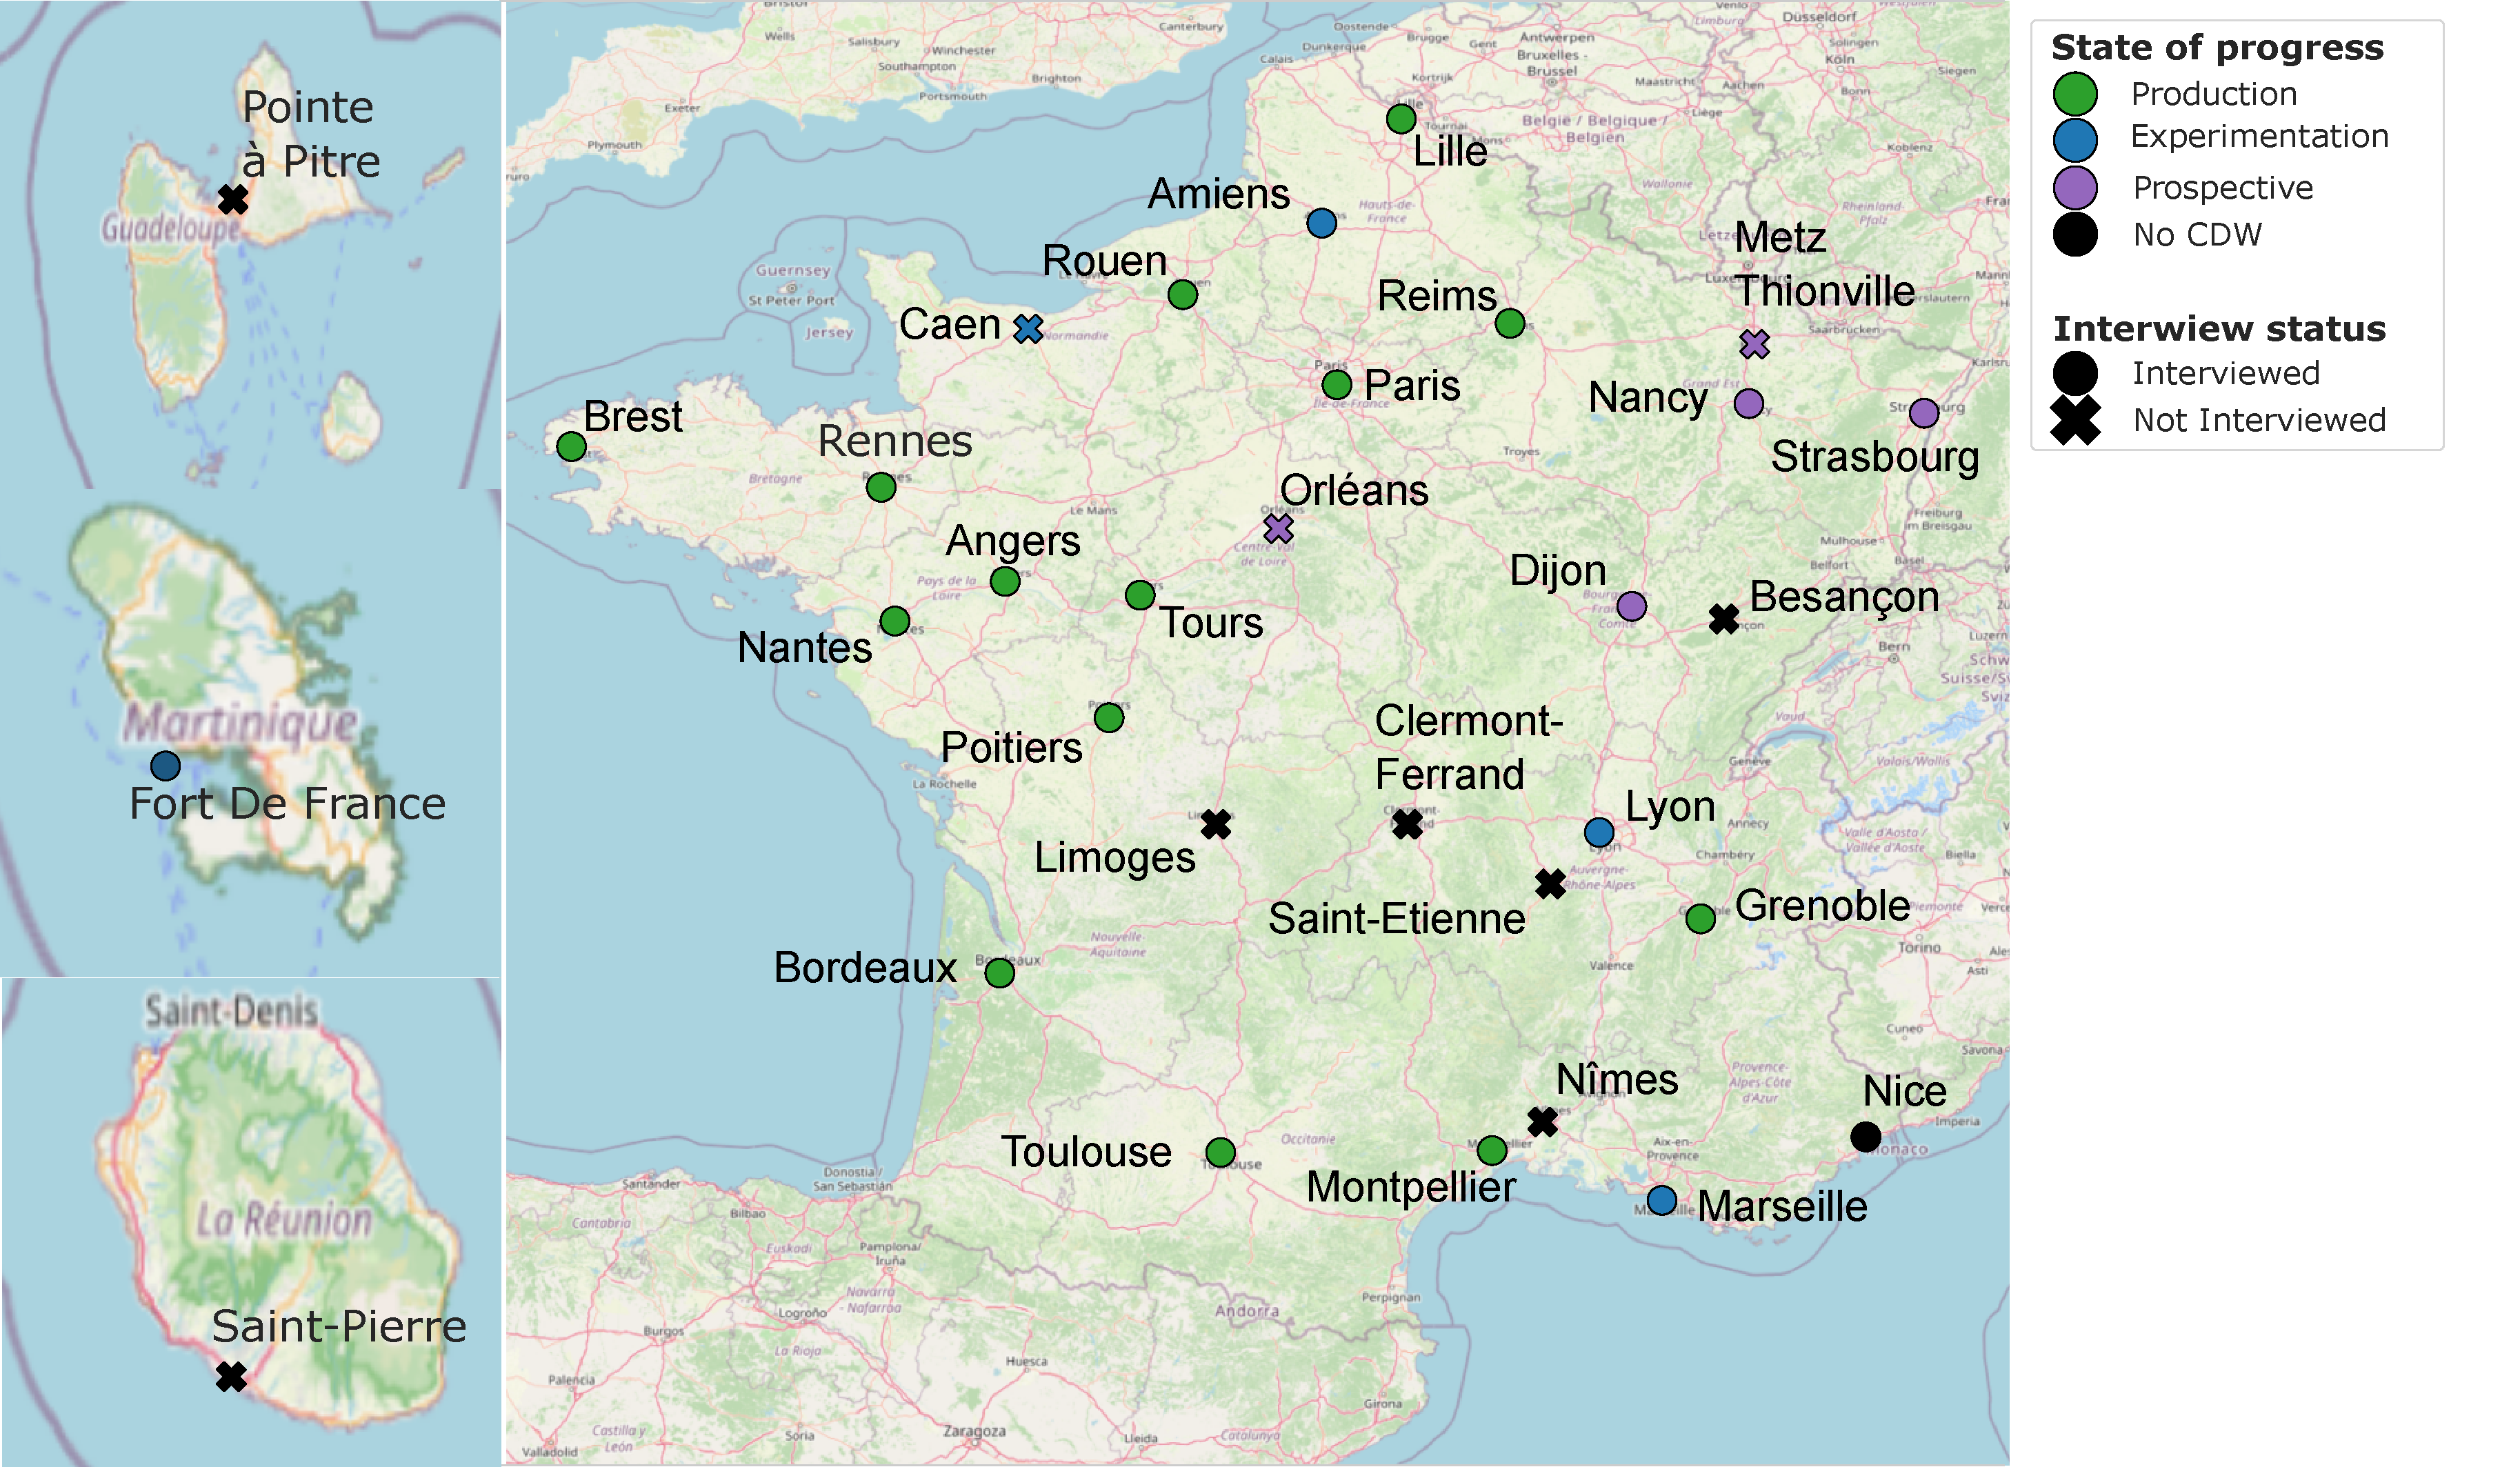
\includegraphics[width=0.82\linewidth]{img/chapter_2/Fig2_thesis.pdf}
  \caption{Repartition of CDWs in France. \\The base layer map comes from
    \url{https://wiki.openstreetmap.org/wiki/Mapnik}.}
  \label{results:image:eds_map}
\end{figure*}


\subsection{Governance: CDWs are federating multiple teams in the hospital}%
\label{subsec:cdw:results:governance}%

\paragraph{Initiation and actors}


Fig \ref{results:governance:image:timeline} shows the history of the
implementation of CDWs. A distinction must be made between the first works --in
blue--, which systematically precede the regulatory authorization --in green--
from the French Commission on Information Technology and Liberties (CNIL).

\begin{figure*}
  \centering
  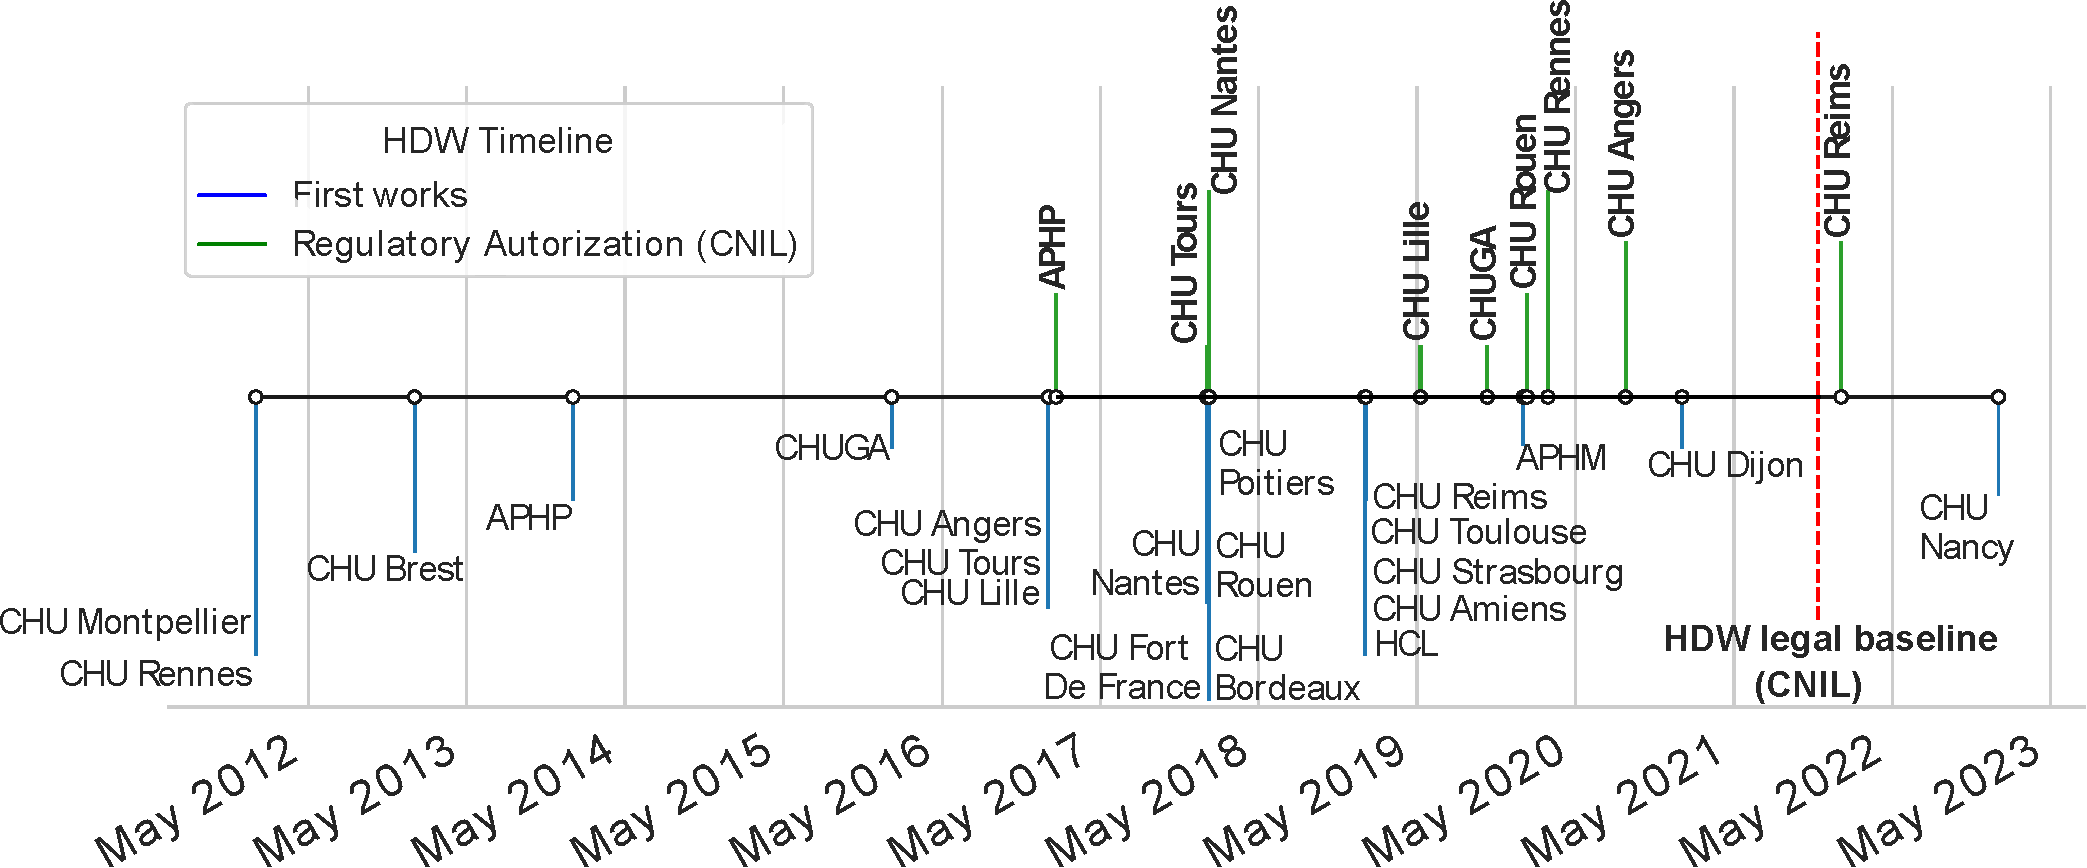
\includegraphics[width=\linewidth]{img/chapter_2/Fig3.pdf}
  \caption{The French CDWs implementations date back to the first academic works in data reuse in early 2010s and accelerated recently.}
  \label{results:governance:image:timeline}
\end{figure*}

The CDWs have so far been initiated by one or two people from the hospital world
with an academic background in bioinformatics, medical informatics or
statistics. The sustainability of the CDW is accompanied by the construction of
a cooperative environment between different actors: Medical Information
Department (MID), Information Systems Department (IT), Clinical Research
Department (CRD), clinical users, and the support of the management or the
Institutional Medical Committee. It is also accompanied by the creation of a
team, or entity, dedicated to the maintenance and implementation of the CDW.
More recent initiatives, such as those of the HCL (Hospitals of the city of
Lyon) or the \textit{Grand-Est} region, are distinguished by an initial,
institutional and high-level support.

The CDW has a federating potential for the different business departments of the
hospital with the active participation of the CRD, the IT Department and the
MID. Although there is always an operational CDW team, the human resources
allocated to it vary greatly: from half a full-time equivalent to 80 people for
the AP-HP, with a median of 6.0 people. The team systematically includes a
coordinating physician. It is multidisciplinary with skills in public health,
medical informatics, informatics (web service, database, network,
infrastructure), data engineering and statistics.

Historically, the first CDWs were based on in-house solution development. More
recently, private actors are offering their services for the implementation and
implementation of CDWs (15/21). These services range from technical
expertise in order to build up the data flows and data cleaning up to the delivery
of a platform integrating the different stages of data processing.

\subsection{Management of studies}

Before starting, projects are systematically analyzed by a scientific and
ethical committee. A local submission and follow-up platform is often mentioned
(12/21), but its functional scope is not well defined. It ranges from simple
authorization of the project to the automatic provision of data into a Trusted
Research Environment (TRE) \citep{goldacre_better_2022}. The processes for
starting a new project on the CDW are always communicated internally but rarely
documented publicly (8/21).

\subsection{Uneven transparency of ongoing studies}%
\label{subsec:cdw:results:transparency}%

Ongoing studies in CDWs are unevenly referenced publicly on hospital websites.
Some institutions have comprehensive study portals, while others list only a
dozen studies on their public site while mentioning several hundreds ongoing
projects during interviews. In total, we found 8 of these portals out of 14 CDWs
in production. Uses other than ongoing scientific studies are very rarely
documented. The publication of the list of ongoing studies is very heterogeneous
and fragmented between several sources: \url{clinicaltrials.gov}, the mandatory
project portal of the Health Data Hub \citep{health_data_hub_portal_2023} or the
website of the hospital data warehouse.

\subsection{Triple usage of data: Research, management, clinic}%
\label{subsec:cdw:results:data}%

\paragraph{Strong dependance to the Hospital Information System}

CDW data reflect the HIS used on a daily basis by hospital staff. Stakeholders
point out that the quality of CDW data and the amount of work required for rapid
and efficient reuse are highly dependent on the source HIS. The possibility of
accessing data from an HIS in a structured and standardized format greatly
simplifies its integration into the CDW and then its reuse.

\paragraph{Categories of Data}

Although the software landscape is varied across the country, the main
functionalities of HIS are the same. We can therefore conduct an analysis of the
content of the CDWs, according to the main categories of common data present in
the HIS.

The common base for all CDWs is constituted by data from the Patient
Administrative Management software (patient identification, hospital movements)
and the billing codes. Then, data flows are progressively developed from the
various softwares that make up the HIS. The goal is to build a homogeneous data
schema, linking the sources together, controlled by the CDW team. The
prioritization of sources is done through thematic projects, which feed the CDW
construction process. These projects improve the understanding of the sources
involved, by confronting the CDW team with the quality issues present in the
data.

Table \ref{results:data:img:data_categories} presents the different ratio of
data categories integrated in French CDWs. Structured biology and texts are
almost always integrated (20/21 and 20/21). The texts contain a large amount of
information. They constitute unstructured data and are therefore more difficult
to use than structured tables. Other integrated sources are the hospital drug
circuit (prescriptions and administration, 16/21), Intense Care Unit (ICU, 2/21)
or nurse forms (4/21). Imaging is rarely integrated (4/21), notably for reasons
of volume. Genomic data are well identified, but never integrated, even though
they are sometimes considered important and included in the CDW work program.


\begin{minipage}{0.45\textwidth}
  \begin{table}[H]
    \centering
    \resizebox*{\textwidth}{!}{
      \begin{tabular}{lrl}
        \thickhline
        Category of data     & Number of CDW & Ratio  \\
        \thickhline
        Administrative       & 21            & 100 \% \\
        Billing Codes        & 20            & 95 \%  \\
        Biology              & 20            & 95 \%  \\
        Texts                & 20            & 95 \%  \\
        Drugs                & 16            & 76 \%  \\
        Imagery              & 4             & 19 \%  \\
        Nurse Forms          & 4             & 19 \%  \\
        Anatomical pathology & 3             & 14 \%  \\
        ICU                  & 2             & 10 \%  \\
        Medical devices      & 2             & 10 \%  \\
        \thickhline
      \end{tabular}
    }
    \caption{Type of data integrated into the French CDWs.}
    \label{results:data:img:data_categories}
  \end{table}
\end{minipage}
\begin{minipage}{0.5\textwidth}
  \begin{figure}[H]
    \centering
    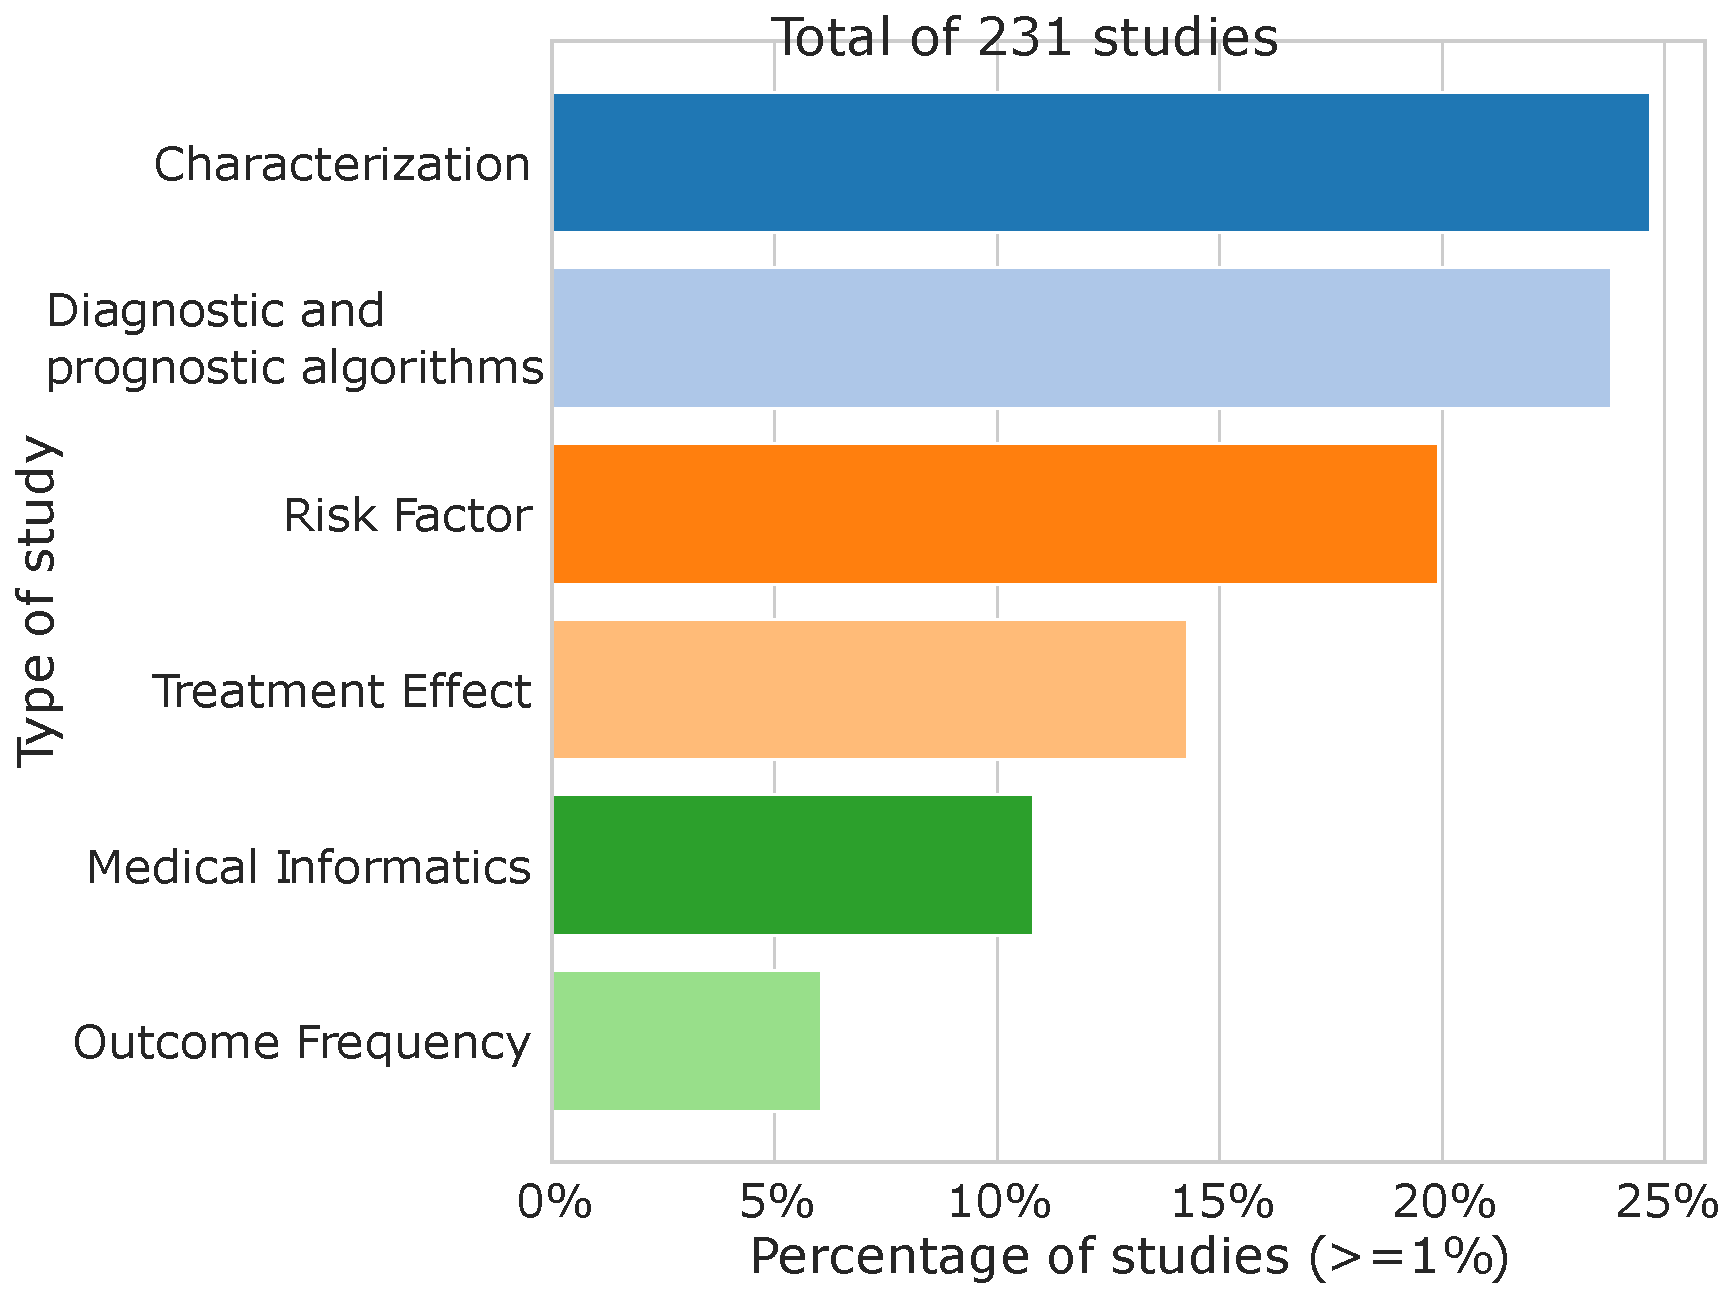
\includegraphics[width=\linewidth]{img/chapter_2/Fig4.pdf}
    \caption{Percentage of studies by objective.}
    \label{results:usage:image:study_objective}
  \end{figure}
\end{minipage}

\paragraph{Today, CDWs are built predominantly for scientific research (21/21)}

The studies are mainly observational (non-interventional). Fig
\ref{results:usage:image:study_objective} presents the distribution of the six
categories defined in \ref{subsec:cdw:classification} for 231 studies collected
on the study portals of nine hospitals. The studies focus first on population
characterization (25 \%), followed by the development of decision support
processes (24 \%), the study of risk factors (19 \%) and the treatment effect
evaluations (15 \%).


The CDWs are used extensively for internal projects such as student theses (at
least in 9/21) and serve as an infrastructure for single-service research: their
great interest being the de-siloing of different information systems. For most
of the institutions interviewed, there is still a lack of resources and maturity
of methods and tools for conducting inter-institutional research (such as in the
\textit{Grand-Ouest} region of France) or via European calls for projects
(EHDEN). These two research networks are made possible by supra-local governance
and a common data schema, respectively eHop \citep{madec_ehop_2019} and OMOP
\citep{hripcsak_observational_2015}. The Paris hospitals, thanks to their
regional coverage and the choice of OMOP, are also well advanced in multi-centric
research. At the same time, the \textit{Grand-Est} region is building a network
of CDW based on the model of the \textit{Grand-Ouest} region, also using eHop.

\paragraph{Data reuse: CDW are used for monitoring and management (16/21)}


The CDW have sometimes been initiated to improve and optimize billing coding
(4/21). The clinical texts gathered in the same database are queried using
keywords to facilitate the structuring of information. The data are then
aggregated into indicators, some of which are reported at the national level.
These types of indicators also inform the administrative management of the
institution. Finally, closer to the clinic, some actors state that the CDW could
also be used to provide regular and appropriate feedback to healthcare
professionals on their practices. This feedback would help to increase the
involvement and interest of healthcare professionals in CDW projects. The CDW is
sometimes of interest for health monitoring (eg. during Covid-19) or
pharmacovigilance (13/21).


\paragraph{Data reuse: Strong interest for CDW in the context of care (13/21)}

Some CDWs develop specific applications that provide new functionalities
compared to care software. Search engines can be used to query all the
hospital's data gathered in the CDW, without data compartmentalization between
different softwares. Dedicated interfaces can then offer a unified view of the
history of a patient's data, with inter-specialty transversality, which is
particularly valuable in internal medicine. These cross-disciplinary search
tools also enable healthcare professionals to conduct rapid searches in all the
texts, for example to find similar patients \citep{garcelon_finding_2017}. Uses
for prevention, automation of repetitive tasks and care coordination are also
highlighted. Concrete examples are the automatic sorting of hospital
prescriptions by order of complexity, or the setting up of specialized channels
for primary or secondary prevention.
%
%There is a growing interest in such computational phenotyping tools to support
%the development of digital health solutions \citep{wen2023impact}.

\subsection{A multi-layered technical architecture}%
\label{subsec:cdw:results:architecture}%


The technical architecture of modern CDWs has several layers:
\begin{itemize}
  \item Data processing: connection and export of source data, diverse
        transformation (cleaning, aggregation, filtering, standardization).
  \item Data storage: database engines, file storage (on file servers or object
        storage), indexing engines to optimize certain queries.
  \item Data exposure: raw data, APIs, dashboards, development and analysis
        environments, specific web applications.
\end{itemize}
Supplementary cross-functional components ensure the efficient and secure
operation of the platform: identity and authorization management, activity
logging, automated administration of servers and applications.

The analysis environment (Jupyterhub or RStudio datalabs) is a key component of
the platform, as it allows data to be processed within the CDW infrastructure. A
few CDWs had such operational datalab at the time of our study (6/21) and almost
all of them have decided to provide it to researchers. Currently, clinical
research teams are still often working on data extractions, in less secure
environments.

\subsection{Rare data quality checks and multiple standard formats}%
\label{subsec:cdw:results:data_quality}%

\paragraph{Quality tools}

Systematic data quality monitoring processes are
being built in some CDWs. Often (8/21), scripts are run at regular intervals to
detect technical anomalies in data flows. Rare data quality investigation tools,
in the form of dashboards, are beginning to be developed internally (3/21).
Theoretical reflections are underway on the possibility of automating data
consistency checks, for example, demographic or temporal. Some facilities
randomly pull records from the EHR to compare them with the information in the
CDW.

\paragraph{Standard format}

No single standard data model stands out as being used by all CDWs. All are
aware of the existence of the OMOP (research standard)
\citep{hripcsak_observational_2015} and HL7 FHIR (communication standard) models
\citep{braunstein_health_2019}. Several CDWs consider the OMOP model to be a
central part of the warehouse, particularly for research purposes (9/21). This
tendency has been encouraged by the European call for projects EHDEN, launched
by the OHDSI research consortium, the originator of this data model. In the
\textit{Grand-Ouest} region of France, the CDWs use the eHop warehouse software.
The latter uses a common data model also named eHop. This model will be extended
with the future warehouse network of the  \textit{Grand Est} region also
choosing this solution. Including this grouping and the other establishments
that have chosen eHop, this model includes 12 establishments out of the 32
university hospitals. This allows eHop adopters to launch ambitious
interregional projects. However, eHop does not define a standard nomenclature to
be used in its model and is not aligned with emerging international standards.

\paragraph{Documentation}

Half of the CDWs have put in place documentation accessible within the
organization on data flows, the meaning and proper use of qualified data (10/21
mentioned). This documentation is used by the team that develops and maintains
the warehouse. It is also used by users to understand the transformations
performed on the data. However, it is never publicly available. No schema of the
data once it has been transformed and prepared for analysis is published.

\section{Recommendations: How to consolidate EHRs and expand usages}%
\label{sec:cdw:recommendations}%

We give the first overview of the CDWs in university hospitals of France with 32
hospitals reviewed. The implementation of CDW dates from 2011 and accelerated in
the late 2020. Today, 24 of the university hospitals have an ongoing CDW
project.
From this case study, some general considerations can be drawn, that should be
valuable to all healthcare system implementing CDWs on a national scale.


\subsection{Governance: CDWs are infrastructures}%
\label{subsec:cdw:recommendations:governance}%

\paragraph{Multidisciplinar teams} As the CDW becomes an essential component of data management in the hospital,
the creation of an autonomous internal team dedicated to data architecture,
process automation and data documentation should be encouraged
\citep{goldacre_better_2022}. This multidisciplinary team should develop an
excellent knowledge of the data collection process and potential reuses in order
to qualify the different flows coming from the source IS, standardize them
towards a homogenous schema and harmonize the semantics. It should have a sound
knowledge of public health, as well as the technical and statistical skills to
develop high-quality software that facilitates data reuse.

\paragraph{Lack of sustainable fundings} The resources specific to the warehouse are rare and often taken from other
budgets, or from project-based credits. While this is natural for an initial
prototyping phase, it does not seem adapted to the perennial and transversal
nature of the tool. As a research infrastructure of growing importance, it must
have the financial and organizational means to plan for the long term.

\paragraph{The governance of the CDW has multiple layers:} local within the
university hospital, interregional, and national/international. The first level
allow to ensure the quality of data integration as well as the pertinence of
data reuse by clinicians themselves. The interregional level is well adapted for
resources mutualization and collaboration. Finally, the national and
international levels assure coordination, encourage consensus for committing
choices such as metadata or interoperability, and provide financial, technical
and regulatory support.


\subsection{Transparency: Keep the bar high}%
\label{subsec:cdw:recommendations:transparency}%

\paragraph{For better registration of observational studies:} Health Technology
Assessment agencies advocate for public registration of comparative
observational study protocols before conducting the analysis
\citep{berger2017good,fda_real-world_2021,has_real-world_2021}. They often refer
to \url{clinicaltrials.gov} as potential but not ideal registration portal for
observational studies. The research community advocates for public registrations
of all observational studies \citep{rushton2011should,plos2014observational}.
More recently, it emphasizes the need for more easy data access and the
publication of study code
\citep{pavlenko_implementation_2020,kohane_what_2021,nih_2023}. We embrace these
recommendations and we point to the unfortunate duplication of these study
reporting systems in France. One source could be favored at the national level
and the second one automatically fed from the reference source, by agreeing on
common metadata.

\paragraph{From a patient's perspective,} there is currently no way to know if
their personal data is included for a specific project. Better patient
information about the reuse of their data is needed to build trust over the long
term. A strict minimum is the establishment and update of the declarative
portals of ongoing studies at each institution.

\subsection{New data, new challenges}%
\label{subsec:cdw:recommendations:data}%

\paragraph{Shift the focus to data engineering} When using CDW, the analyst has not defined the data collection process and is
generally unaware of the context in which the information is logged. This new
dimension of medical research requires a much greater development of data
science skills to change the focus from the implementation of the statistical
design to the data engineering process. Data reuse requires more effort to
prepare the data and document the transformations performed.

\paragraph{Poor adoption of common standards} The more heterogeneous a HIS system is, the less qualitative would be the CDW
built on top of it. There is a need for increasing interoperability, to help EHR
vendors interfacing the different hospital softwares, thus facilitating CDW
development. One step in this direction would be the open source publication of
HIR data schema and vocabularies. At the analysis level, international recommendations insist
on the need for common data formats \citep{zhang_best_2022,kohane_what_2021}.
However, there is still a lack of adoption of research standards from hospital
CDWs to conduct robust studies across multiple sites. Building open-source tools
on top of these standards such as those of OHDSI \citep{schuemie_book_2021} could
foster their adoption. Finally, in many clinical domains, sufficient sample size
is hard to obtain without international data sharing collaborations. Thus, more
incitation is needed to maintain and update the terminology mappings between
local nomenclatures and international standards.

\paragraph{Lack of translational researches} Many ongoing studies concern the development of decision support processes whose
goal is to save time for healthcare professionals. These are often research
projects, not yet integrated into routine care. The analysis of study portals
and the interviews revealed that data reuse oriented towards primary care is
still rare and rarely supported by appropriate funding. The translation from
research to clinical practice takes time and need to be supported on the long
run to yield substantial results.

\subsection{Technical architecture: Towards more harmonization and open source
  ?}%
\label{subsec:cdw:recommendations:architecture} %

Tools, methods and data formats of CDW lack harmonization due the presence of
many actors. The strong technical innovation in the field led to the emergence
of many heterogeneous solutions. As suggested by the recent report on the use of
data for research in the UK \citep{goldacre_better_2022}, it would be wise to
focus on a small number of model technical platforms.

These platforms should favor open-source solutions to assure transparency by
default, foster collaboration and consensus and avoid technological lock-in of
the hospitals.
%\md{More on open-source from the french version of the report? }
% Case for open source: transparency, less technological lock-in, mutualization,
% favor modularity, help build consensus Opportunity for open source solutions

\subsection{Data quality an documentation: more incentives needed}%
\label{subsec:cdw:recommendations:quality}%

\paragraph{Focus on data quality} Quality is not sufficiently considered as a relevant scientific topic itself.
However, it is the backbone of all research done within an CDW. In order to
improve the quality of the data with respect to research uses, it is necessary
to conduct continuous studies dedicated to this topic
\citep{zhang_best_2022,kohane_what_2021,shang_conceptual_2018,looten_what_2019}.
These studies should contribute to a reflection on methodologies and standard
tools for data quality, such as those developed by the OHDSI research network
\citep{schuemie_book_2021}.

\paragraph{Open-source is key to improve quality} Finally, there is a need for
open-source publication of research code to ensure quality retrospective
research \citep{shang_conceptual_2018,seastedt_global_2022}. Recent research in
data analysis has shown that innumerable biases can lurk in training data sets
\citep{gebru_datasheets_2021,mehrabi_survey_2021}. Open publication of data
schemas is considered an indispensable prerequisite for all data science and
artificial intelligence uses \citep{gebru_datasheets_2021}. Inspired by dataset
cards \citep{gebru_datasheets_2021} and dataset publication guides, it would be
interesting to define a standard CDW card documenting the main data flows.

\section{Conclusion}\label{sec:cdw:conclusion}

\paragraph{Limitations}

The interviews were conducted in a semi-structured manner within a limited time
frame. As a result, some topics were covered more quickly and only those
explicitly mentioned by the participants could be recorded. The uneven existence
of study portals introduces a bias in the recording of the types of studies
conducted on CDW. Those with a transparency portal already have more maturity in
use cases.

For clarity, our results are focused on the perimeter of university hospitals.
We have not covered the exhaustive health care landscape in France. CDW
initiatives also exist in primary care, in smaller hospital groups and in
private companies.

\paragraph{The French CDW ecosystem is beginning to take shape,} benefiting from
an acceleration thanks to national funding, the multiplication of industrial
players specializing in health data and the beginning of a supra-national
reflection on the European Health Data Space \citep{ehds_2022}. However, some
points require special attention to ensure that the potential of the CDW
translates into patient benefits.

\paragraph{The priority is the creation and perpetuation of multidisciplinary
  warehouse teams} capable of operating the CDW and supporting the various
projects. A combination of public health, data engineering, data stewardship,
statistics and IT competences is a prerequisite for the success of the CDW. The
team should be the privileged point of contact for data exploitation issues and
should collaborate closely with the existing hospital departments.

\paragraph{The constitution of a multi-level collaboration network} is another
priority. The local level is essential to structure the data and understand its
possible uses. Interregional, national and international coordination would make
it possible to create thematic working groups, in order to stimulate a dynamic
of cooperation and mutualization.

\paragraph{A common data model should be encouraged,} with precise metadata allowing to map
the integrated data, in order to qualify the uses to be developed today from the
CDWs. More broadly, open-source documentation of data flows and transformations
performed for quality enhancement would require more incentives to unleash the
potential for innovation for all health data users.

\paragraph{Expanding the scope of the data beyond the purely hospital domain}
in a systematic way should be considered. Many risk factors and patient
follow-up data are missing from the CDWs, but are crucial for understanding
pathologies. Combining city data and hospital data would provide a complete view
of patient care.


%%%%%%%%%%%%%%%%%%%%%% CHAPTER 3 %%%%%%%%%%%%%%%%%%%%%%

\chapter{Exploring a complexity gradient in representation and predictive algorithms for EHRs}\label{chapter:predictive_models}

\begin{citationbox}
  What must one know a priori about an unknown functional dependency in order to
  estimate it on the basis of observations?
  \par\hfill -- Vladimir Vapnik, \textit{The nature of Statistical Learning Theory (2000)}
\end{citationbox}

\begin{chapterabstract}\label{sec:predictive_models:abstract}%
  As chapter \ref{chapter:cdw} shows, Electronic Health Records (EHRs) contain
  multiple categories of data that sparkle interest in the development of
  predictive prognosis. Text and image data put apart, these data elements can
  be represented as timed events with high cardinality encoded in medical codes.
  Current state-of-the-art predictive models for EHRs build on increasingly
  elaborated pipelines --based on the transformer architecture-- to handle the
  complexity of these data. Acknowledging the difficulty to deploy, transfer and
  adapt these models on local care environments, we explore a complexity-benefit
  tradeoff by comparing them to simple aggregation of events. We use three
  predictive tasks involving time-varying structured EHRs and increasingly
  clinically relevant problems. We show that these benchmarking tasks display
  heterogeneous predictive difficulties. We introduce a simple aggregation of
  static embeddings --transferred from national claims and publicly available--,
  showing that it outperforms transformer-based models on simple tasks with
  medium sample sizes. We highlight the sample and computing resource efficiency
  of these models. Finally, clinically relevant problems generally present a
  strong class imbalance, which complicates models development and undermines
  their performances. Further work is needed to understand if transformer-based
  models perform well in these scenarios where the number of cases requires good
  sample efficiency.
\end{chapterabstract}


\vfill
\begin{flushright}
  \begin{minipage}{15cm}
    {\small{This chapter presents ongoing work. A communication was accepted for
        the Simpa2023 day on patient similarity.}}\\

    {\small\hfill{} work done with Jean-Baptiste \textsc{Julla}, Julie
    \textsc{Adjerad}, Theo \textsc{Jolivet}, Judith \textsc{Abecassis},, Louis
    \textsc{Potier} and Gaël \textsc{Varoquaux}.}
  \end{minipage}
\end{flushright}


\clearpage
\minitoc

\section{The modern quest for medical oracles}%
\label{sec:predictive_models:motivation}%

%But why such interest in predictive pipelines for healthcare ? How these tasks
%relate to th}%
% \label{subsec:predictive_models:importance}%
\gv{I wonder if this is the right way to angle our paper. It seems to me beside
  the points that we are trying to make (but maybe I've just missing the
  angle)}\md{The shift towards less relevant tasks is outside the scope indeed.
  I focused rather on a range of tasks covering a more or less precise clinical
  population. Our point is to benchmark the different models on these different
  type of tasks.}

% promises
Increasing availability of routine care data and progress in
machine learning, have brought much hope in predictive modeling for healthcare.
The richness of the data in EHRs and their integration in routine care make them
a promising application area \citep{raghupathi2014big}.

Benchmarking these models is not easy due to the wide range of potential use
cases.
% However, there is a shift from clinically meaningful objectives towards abstract
% outcomes in EHR predictive modeling literature.
In biostatistics and clinical medicine, prognosis models have been motivated by
\emph{risk stratification}: the Framingham risk score for coronary heart disease
was an early attempt to characterize behavior changes that could lead to
decreased risk \citep{brand1976multivariate}. Clinical \emph{risk scores} are
either focused on the short term with alarm models
\citep{tang2007global,rothman2013development,wong2021external} or on the long
term with screening models. In parallel, artificial intelligence in medicine
looks for prognosis model as part of larger \emph{decision-making} systems
\citep{Szolovits1982artificial}. In complex healthcare organizations, accurate
individual predictions help to use efficiently constrained medical resource by
informing \emph{care planning} \citep{topol2019high}. Appendix
\ref{apd:review_tasks} details these four type of predictive objectives for
healthcare.

Following the trend for evaluating current state-of-the-art models
\citep{wornow2023shaky}, we focus on purely predictive models --risk scores or
planning-- with three tasks ranging from general populations of patients to
more specific clinical cases.

\subsection{Predictive pipelines fueling medical predictions are increasingly
  complex}%
\label{subsec:predictive_models:complex_data}%

This complexity stems from predictive models trying to model ever richer data
sources.

\paragraph{Original complexity of the data}
\gv{Can you make this paragraph a bit shorter: it is not the center of
  our contribution}
\md{better?}
% Big observational databases are complex but contain interesting information
EHRs contain time varying variables with a high cardinality. Time-consuming work
from medical and computer experts is required to clean and transform these
sources into data tables suited for statistical analysis
\citep{bacry2020scalpel3,hripcsak2015observational}. More specifically, data
preprocessing usually requires to map non standard terminologies, create derived
variables by aggregating measures over specific time periods. The choices of
baseline covariates should be driven by medical experts which are often not
familiar the complexity of the EHR data processing pipeline. We propose to leverage models that takes raw
data as input to avoid as much as possible these preprocessing steps.

%  At the time of study, population
%  inclusion criteria should be aligned with expert conception -- a task known as
%  computational phenotyping \citep{richesson2013electronic,
%  newton2013validation}. 

\paragraph{From simple hand-crafted linear models to elaborated weakly-supervised tranformers}

% increased complexity of models
Predictions on EHRs originally used linear models on few carefully selected
static variables for tens of thousand patients coming from a single center
\citep{goldstein2017opportunities}. To overcome the high cardinality of EHRs
medical vocabularies, a range of deep learning methods were developed
\citep{shickel2017deep}. Time varying features were first modelled thanks to
recurrent neural network \citep{lipton2016learning}, then with transformer based
architectures \citep{li2020behrt}. Appendix \ref{apd:review_models} further
details this evolution of predictive model complexity.

\subsection{Transfer learning: no silver bullet}%
\label{subsec:predictive_models:low_prevalence}%

\gv{First tell us how we get the small number of datasets. Show us how starting
  from a big data, we get to small data. Then, merge the two paragraph below in
  a smaller, shorter one "Transfer learning: no silver bullet". Make it shorter,
  because right now you are putting a lot of words on it, so you are drawing
  attention to it, and you are going to prime the reader to ask you to compare
  to it (actually, I wonder whether this should not be moved to the
  discussion)}\md{Is it better ? I moved to the discussion the interrogation on
  the performances of large transformer models and added the concrete example
  for small number of cases.}

% Low prevalence
%\paragraph{Transferring to new tasks still requires a high number of cases }
Well-defined clinical questions concern a very small number of cases --diseases
are rare, often with less than 5\% of prevalence. For example, consider the
prediction of cardiovascular complications --a rather common clinical
condition--, we first extracted a cohort of 2,101,819 patients. After running
all inclusion criteria --shown in Figure \ref{apd:fig:flowchart_t3}, we are left
with only 4,360 cases among a population at risk of 165,930 patients. Currently,
large models are trained on larger number of cases (see a review of number of
cases for three major transformer based models in Appendix
\ref{apd:foundation_model_nb_cases}). Due to the difficulty to access data
linked to privacy rights, we should also compare this to problems with
smaller samples.

% Major dataset shifts
%\paragraph{Transferring predictive pipelines from one data site to another is rarely effective} Due to dataset shifts
%\citep{moreno-torres_unifying_2012,storkey_when_2013,finlayson2021clinician}.
Major dataset shifts make it difficult to transfer predictive
pipelines \citep{finlayson2021clinician}: heterogeneity in coding practices \citep{juven2013codage},
socio-economic status \citep{gianfrancesco2018potential}, inconsistency of
practices in different organizations \citep{agniel2018biases}.
% The small number
% of external evaluations of transformer based models is not sufficient to
% conclude to their transfer capacities.
% Model generalization might not be desirable
It might not even be possible to generalize machine learning models in
healthcare \citep{futoma2020myth}. Different population, information systems and
healthcare practices may require tailored tools \citep{rose2018}. For example,
\cite{wong2021external} evaluated externally a widely deployed sepsis prediction
model showing poor transfer performance of 0.63 ROC AUC.



\subsection{Current barriers to predictive models usefulness}%
\label{subsec:predictive_models:useful}%

\paragraph{Credibility of external validity requires simple model deployments}

Some predictive risks are used in daily clinical practice: For example, the
Glasgow Coma Scale \citep{teasdale1974assessment} or the APACHE III score
\citep{knaus1991apache}. But only a small part of the published models are
successfully deployed into clinical practice \citep{wyatt1995commentary,
  kelly2019key}. Poor adoptions are due to lack of evidence for clinical
credibility, accuracy, generality or clinical effectiveness. Improving the
strength of this evidence requires to repeatedly test these systems on
different prospective populations with intuitive metrics for physicians
\citep{kelly2019key, varoquaux2022evaluating, wornow2023shaky}.

\paragraph{Complex systems and privacy requirements hinders model deployments}
The growing body of predictive models from EHR focus mainly on accuracy
performances. They are rarely shared due to privacy requirements. They are tied
to specific tasks hardcoded into the model architectures
\citep{wornow2023shaky}. The increasing sample and architecture sizes require
ever greater computing and technical resources -- as detailed in Appendix
\ref{apd:computing_resources_review}. These factors lead to models being trained and
evaluated on a small fraction of existing healthcare datasets, endangering
external validity, integration into EHR and ultimately usefulness
\citep{sharma2021,wornow2023shaky}.

There is a need to balance good predictive performances with better clinical
integration, which is tightly linked with simple deployment.

\subsection{Objective and outline of the paper}%
\label{subsec:predictive_models:contribution}%

\paragraph{Contributions}
We study the performances of increasingly complex models on three operational
and clinical tasks. We explore the performance trade-offs between small models
that can be run on few samples and large models requiring more samples to become
efficient. We propose a new model based on the transfer of static medical
embeddings trained from large claims databases. In the technically and legally
constrained environment of healthcare data, what predictive pipelines are the
most efficient to yield good practical utility?

\paragraph{Outline}
Section \ref{sec:predictive_models:pipelines} details four predictive pipelines
of increasing complexity. Subsection
\ref{subsec:predictive_models:task_definitions} define three clinical tasks
covering different benchmarking and clinical usefulness. Subsection
\ref{subsec:predictive_models:evaluation_pipeline} details our evaluation
pipeline. Finally subsection \ref{subsec:predictive_models:results} presents our
results and section \ref{sec:predictive_models:conclusion} discusses their
implications.

\paragraph{Main findings}

With small to moderate sample sizes -up to 10,000 patients-, simple models have
better performances than transformer models on general tasks such as length of
stay or prognosis. Among the simpler model based on row counts or static
embeddings, no featurization choice largely outperforms others in any single
task but random forest estimators are always more performant than linear models.
Static embeddings models are the most compute and memory efficient solution.
Small target prevalence --linked to the number of cases-- is detrimental
to the performances of prognosis models.

%Benchmark tasks are simpler to instantiate but are hard to include into a
%practical medical workflow. 


\section{From basic to complex: four increasingly sophisticated predictive pipelines}%
\label{sec:predictive_models:pipelines}%

\subsection{A simple non destructive data format: sequence of events}%
\label{subsec:predictive_models:event_format}%
% Time-varying features with high cardinality is the specificity and is handled
% by the event data format
We adopt the common modeling of patient healthcare trajectory as a sequence of
events \citep{beam2019clinical, bacry2020scalpel3, chazard2022book}. Each event
is described by a triplet: a person identifier $i$, a datetime $t$ and a medical
code $c$, $e = (i, t, c)$ as shown in Figure \ref{fig:ehr_prediction_timeline}.
For each patient $i$, the complete trajectory is the ordered collection of its
$T_i$ events $\{e_k\}_{k=1..T_i}$. This simple format integrates together a wide
variety of time varying features without imposing data transformation or feature
selection --often brittle to modelization choices. However, it calls for
adequate aggregation methods to reduce the long event table into a patient-wise
features table of shape $N \times d$ matrix for $d$  that can be passed over to
statistical estimators.
% Naive pivot along the concept column yields high dimensional and sparse
% matrices poorly suited to small sample populations, often encountered in
% healthcare application use cases.
Here, we explore four different choices of aggregation of increasing
complexity, followed by common statistical estimators. We call these aggregation
methods \emph{featurizers} and note them $g(\cdot, \lambda_g)$, where
$\lambda_g$ are the parameters of the featurizers.

\begin{figure}
  \centering
  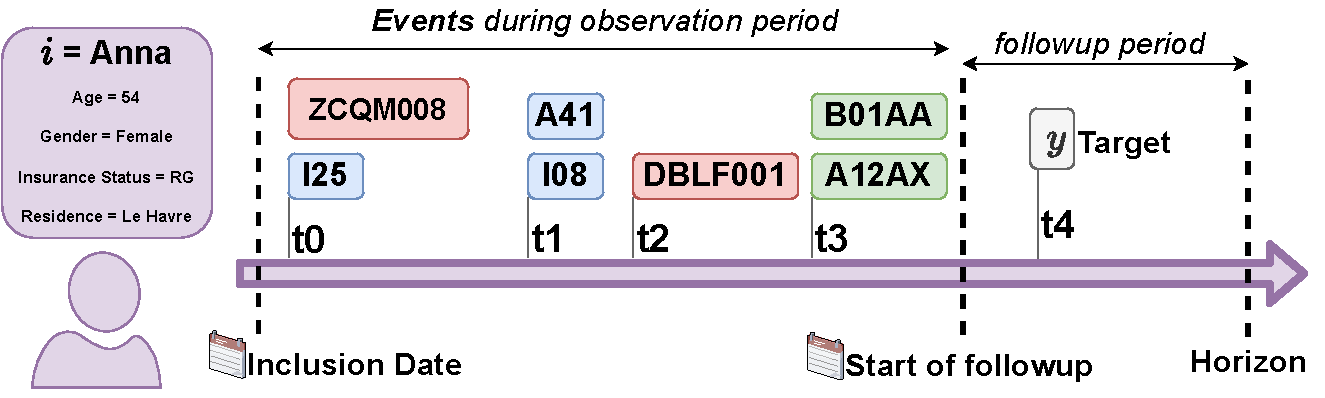
\includegraphics[width=0.8\textwidth]{img/chapter_3/ehr_trajectory_predictive.pdf}
  \caption{Event time representation of EHRs data for predictive tasks. Events
    are observed between the inclusion and start of followup dates. Target is
    considered only between the start of followup and the horizon to avoid right
    censoring. The event types are distinguished by their color: billing
    diagnoses in blue, billing procedures in red and drug administrations in
    green.}\label{fig:ehr_prediction_timeline}
\end{figure}

\subsection{Demographic features: $g_{demo}$}\label{subsec:predictive_models:demographic}

A simple featurization choice --pervasive before machine learning techniques--
considers only a few demographic features available in the patient record: age,
gender, admission origin, discharge destination, admission date.

\subsection{Count encoding of event features: $g_{count}$}\label{subsec:predictive_models:count_encoding}

We process the raw events by computing a sparse count matrix $C$ of shape
$(n_{patients}, n_{vocabulary})$ where each row collapses the patient history by
counting the number of times a concept is present in the patient history. To
better take into account the temporal dimension, we also computed a decayed
count of the events in the patient history, noted $C_{\delta}$. For an event
triplet $(i, t, c)$, we compute the time delta between the event and the followup
time.
$$\Delta t = |t-T_0|$$
Then, we decay the count matrix with an exponential of half life $\delta$.
$$C_{\delta}[i, c] += e^{-\frac{\Delta t}{\delta}}$$% 
Finally, we obtain the patient features by concatenating each
delayed count matrix; eg. with decay 0 and decay $\delta$.
$$g_{count}(X, (0, \delta))= [C_{0}, C_{\delta}]$$% 
Several decays can be selected and concatenated together. The decays are
considered hyperparameters which are selected by cross-validation. Appendix
\ref{apd:pipelines:count_encoding} details this feature processing procedure.

\subsection{Static embeddings of event features: $g_{emb-local}$ or $g_{emb-SNDS}$}

The SVD-PPMI algorithm (introduced by \cite{beam2018big}, detailed in Appendix
\ref{apd:pipelines:static_embeddings}) performs a dimension reduction on the
cooccurrence matrix between each medical concepts. Building upon this algorithm,
we propose two sequence representation techniques. These embeddings are static
by opposition to transformer-based embeddings that adapts to the context.

\paragraph{Static embeddings locally trained: $g_{emb-local}$} We apply the
SVD-PPMI algorithm to the training cohort yielding static embeddings
$\Phi_{local}$. Aggregation at the stay level is done using the same
count matrices as for \ref{subsec:predictive_models:count_encoding} --eventually
with decayed counts: $g_{emb-local}(X, (0, \delta))=[C_{0} \cdot \Phi_{local}, C_{\delta} \cdot \Phi_{local}]$.

\paragraph{Transfer trained static embeddings:} Instead of retraining the
embeddings on the train cohort, we rely on static embeddings $\Phi_{SNDS}$
pre-computed on French national claims data from 3,112,565 patients
\citep{doutrelignerepresentations}. The aggregation is performed similarly as
for count encoding and local embeddings: $g_{emb-SNDS}((X, (0, \delta))) = [C_{0} \cdot \Phi_{SNDS}, C_{\delta} \cdot
  \Phi_{SNDS}]$.

\subsection{Transformer based: $g_{cbert}$}%
\label{subsec:predictive_models:transformer}%

Relying on the transformer architecture \citep{vaswani2017attention}, recent
trajectory modeling algorithms showed promising results for various EHR
prediction tasks \citep{li2020behrt, rasmy2021med,pang2021cehr}. We benchmarked CEHR-BERT
\citep{pang2021cehr}, one of these recent transformer-based models particularly
adapted to our data format.

% pretraining and finetuning
Transformer models are trained in two steps: a) First, pre-train the model on an
auxiliary task using a large database. In our case, this task is a Masked Language
Model (MLM): the network tries to predict the medical concept of randomly masked
events in the sequences. The CEHR-BERT implementation also tries to predict the
type of the next visit. b) Then fine-tune the model on the task of interest. We
use the full train set for pretraining and finetuning. Details on this
architecture are given in Appendix \ref{apd:pipelines:cehr_bert}.


\subsection{Final step estimator}\label{subsec:predictive_models:estimators}

These choices of featurizers are not task-specific. To obtain probabilities of
occurrence for the target, the analyst needs to choose and train an estimator $f$
and its corresponding parameters $\lambda_f$. The prediction is given by the chain of the featurizer and the
estimator: $\hat{y} = f(g(\cdot, \lambda_g), \lambda_f)$.

For CEHR-BERT, the predictor is the final layer of the neural network. It is
trained together with the sequence representations during the fine-tuning step.
For the other featurizers, we create a scikit-learn pipeline
\footnote{\url{https://scikit-learn.org/stable/modules/compose.html\#combining-estimators}}
where a featurizer is followed by an estimator: either a penalized logistic
regression or a random forest. The hyperparameters of the featurizers and
estimators can be cross-validated together. %
We experimented with gradient boosting trees, without observing significant performance gains.


\section{Empirical Study}\label{sec:predictive_models:empirical_study}

\subsection{Three clinical and operational tasks}%
\label{subsec:predictive_models:task_definitions}%

\paragraph{Heathcare database: Paris hospital data warehouse}%
\label{sec:data_extraction}%

We used data extracted from Greater Paris Hospitals (AP-HP) data
warehouse, hosting routine care data from 38 hospitals in the Paris area.
Details on this database is given in Appendix \ref{apd:database_description}. We
include every medical event among drug administrations, ICD10 diagnosis and
procedure billing codes. We also add selected static features at the stay level:
age at hospitalization, gender, admission reason.

\paragraph{Correctly framing the prediction task} General workflows describe key
steps to develop predictive models with good practical utility
\citep{ohdsi2019book,tomavsev2021use,jiang2023health}. Here, we detail our
framework to precisely define each task. First, we define a \emph{study period}
during which data acquisition was sufficiently stable. Then, we define and
select the \emph{cohort} detailed for each task. Inclusion criteria are detailed
in the flowcharts of Figure \ref{apd:fig:flowcharts}. We define
the task outcome with: an \emph{index visit}, an \emph{observation period}
during which events are fed to the predictive model, an \emph{horizon} after the
end of the observation period defining the followup, and a target event potentially occurring
during the followup.

We study three tasks of increasing clinical value and implementation complexity
with decreasing benchmark interest. Table \ref{table:predictive_tasks_summary}
summarizes key characteristics of the cohorts and task definitions.

\begin{table}[!ht]
  \centering
  \resizebox*{0.8\textwidth}{!}{

    \begin{tabular}{|l|l|l|l|}
      \hline
      \textbf{}                   & \textbf{Long LOS}                     & \textbf{Prognosis}                  & \textbf{MACE} \\ \hline
      \textbf{Task}               & Binary classification                 & \makecell[l]{Multi-Label                            \\binary classification}                                       & Binary classification                             \\ \hline
      \textbf{Index Visit}        & First inpatient visit                 & Random Non-Final Visit              & Random Visit  \\ \hline
      \textbf{Observation Period} & Index visit                           & \makecell[l]{Full trajectory before                 \\end of index visit}                           & \makecell[l]{Full Ttrajectory before\\end of index visit} \\ \hline
      \textbf{Horizon}            & End of index visit                    & End of next visit                   & 12 Months     \\ \hline
      \textbf{Median Age}         & 56.4                                  & 61.5                                & 60.0          \\ \hline
      \textbf{Female}             & 54.6\%                                & 53.3\%                              & 53.7          \\ \hline
      \textbf{Cohort Size}        & 27,053                                & 10,786                              & 165,948       \\ \hline
      \textbf{Prevalence}         & 23.1\%                                & From 1.3 to 55.9\%                  & 2.6 \%        \\ \hline
      \textbf{Number of cases}    & 6,249                                 & From 139 to 6,029                   & 4,315         \\ \hline
      \textbf{Description}        & \makecell[l]{Long stay classification                                                       \\ (longer than 7 days)} & \makecell[l]{Next stay prognosis:\\ICD10 chapter classification} & \makecell[l]{MACE Prognosis\\at one year}                                      \\ \hline
    \end{tabular}
  }
  \vspace{1em}%
  \caption{Tasks definitions and cohort characteristics.}%
  \label{table:predictive_tasks_summary}%
\end{table}

\paragraph{Plan -- Long Length Of Stay interpolation
  (LOS)}\label{par:task_definitions:los}%
% los justification
During complete hospitalization, stays with extreme LOS values are responsible
for a large share of hospital costs and resource uses. The ability to predict
extreme LOS is useful for resource managements
\citep{omachonu2004predicting,caetano2014data,jiang2023health}.
% los definition
We define LOS as a binary task categorizing each inpatient stay as long if LOS
greater than 7 days or short if LOS shorter than 7 days. Appendix
\ref{apd:task_details:los} details the task definition.

\paragraph{Stratify -- Prognosis prediction}\label{par:task_definitions:prognosis}%%
% prognosis justification
Prognosis is important for prevention as it can influence shared decision-making
between the clinician and the patient.
% prognosis definition
We define a proxy for prognosis as a multi-label binary classification task
where we predict the next stay ICD10 codes starting from a random non final stay
for each patient. We reduce the granularity of the codes to only 21 chapters
at the highest level of the hierarchy. Appendix \ref{apd:task_details:prognosis}
details the task definition. For this task, we realized that providing the index
stay ICD10 chapters was a strong baseline. We
therefore concatenated these codes as separated demographic features for all
pipelines after aggregation.

\paragraph{Prevent -- Predict Major Adverse Cardiovascular Events}\label{par:task_definitions:mace}

% MACE justification
Prediction of all-chapters billing codes does not focus on a clinically
well-defined population. On the contrary, the composite outcome of Major Adverse
Cardiovascular Events (MACE) is often used in clinical trials targets the
cardio-vascular risk.
% MACE definition
We define MACE prediction as the prognosis of incident MACE at one year for a
randomly chosen stay for each patient. Appendix \ref{apd:task_details:mace}
details the task definition.

% remark on low prevalence
For well-defined clinical tasks such as MACE, the study population is only a
small part of the initial general population. Even when studying regional data
warehouses, the relevant population for the algorithm is an order of magnitude
smaller than the full population, requiring better sample efficiency than
general tasks such as LOS or prognosis.


\subsection{Evaluation procedure}\label{subsec:predictive_models:evaluation_pipeline}

We split each cohort obtained in Sub-section
\ref{subsec:predictive_models:task_definitions} into a train and a test set
following a temporal split based on inclusion date with a 0.8/0.2 ratio (Split
detailed in Appendix \ref{apd:evaluation_procedure}). Each patient only
appears in one of the two sets. To study the sample efficiency of the different
pipelines, we further restrict the effective train set size to increasing ratio
of its full size: $N_{train, r}= r \cdot N_{\mathcal{T}} \quad with \quad r \in
  [0.1, 0.25, 0.5, 0.9, 1]$. Figure \ref{fig:evaluation_procedure} summarizes the
procedure.

\begin{figure}[!h]
  \centering
  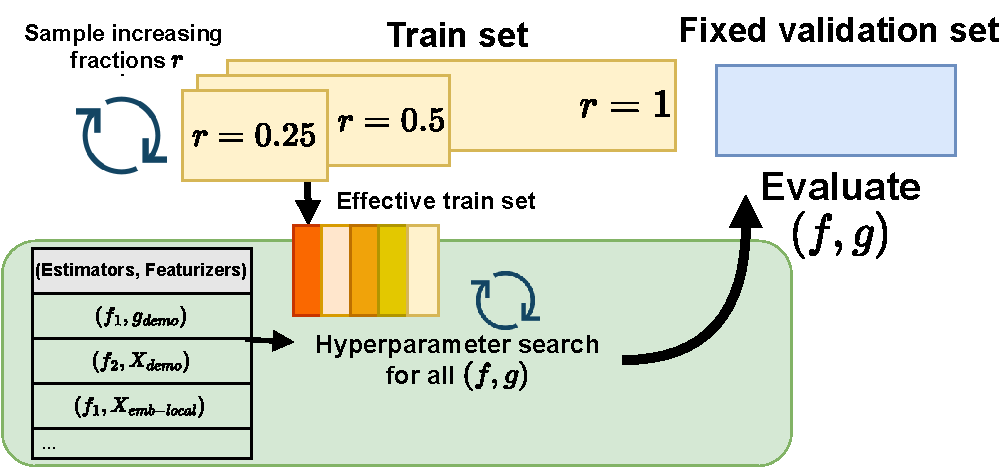
\includegraphics[width=0.7\linewidth]{img/chapter_3/selection_procedure.pdf}
  \caption{Evaluation procedure for non deep learning estimators: For each
    effective train set of size $r$, each pair of featurizer and estimator are
    cross-validated together to obtain the best parameters, then evaluated on a
    fixed validation set.}\label{fig:evaluation_procedure}
\end{figure}

Appendix \ref{apd:hospital_split} details an alternative geographic split
validation procedure for LOS and prognosis tasks, exploring the validity of our
results when testing the models on patient from other hospitals. We report Area
Under the Receiver Operating Characteristic Curve (ROC AUC) and refer to
appendices for brier score and average precision results (AUPRC).


\subsection{Results: Performance-sample
  trade-offs}\label{subsec:predictive_models:results}


\paragraph{Long LOS interpolation: saturating a simple task already requires
  10,000 samples}%


Figure \ref{fig:los_roc_auc} shows that ROC AUC performances for LOS saturates
at 95\% ROC AUC for random forests and every featurizers but the demographics.
The transformer model is not able to reach the best performances, certainly
because of the lack of samples.


\begin{figure}[!h]
  \centering
  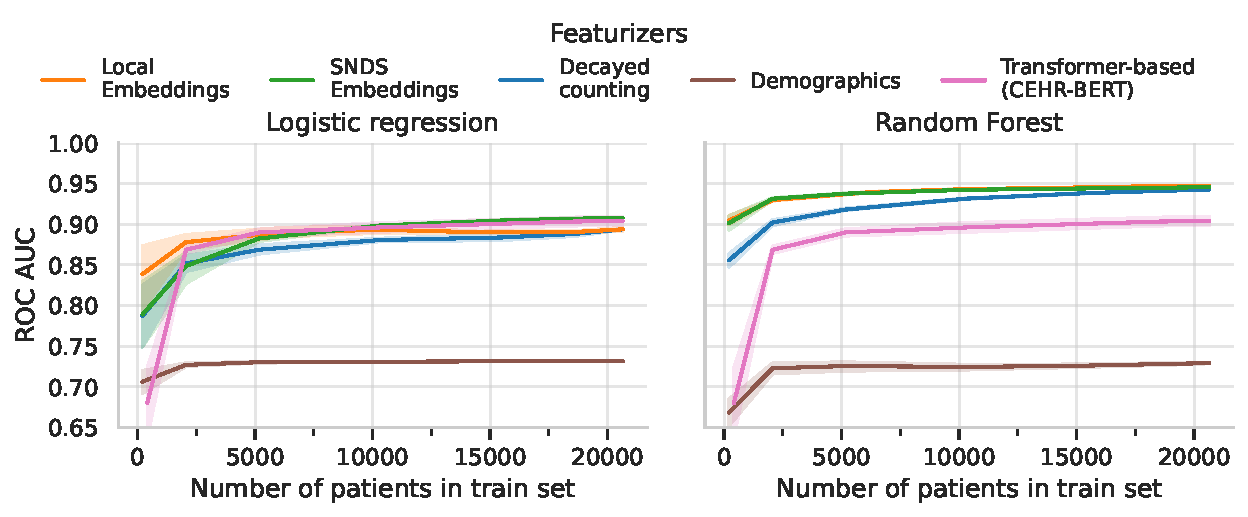
\includegraphics[width=\linewidth]{img/chapter_3/los/roc_auc_score_performances.pdf}
  \caption{LOS ROC AUC for different featurizers and estimators. The
    performances are averaged over 5 folds. The shaded area represents the
    standard deviation. The task performance seems to saturate at 95\% ROC AUC
    for random forest and all featurizers but the demographics and CEHR-BERT,
    suggesting that the Bayes error rate is reached. However, for lower sample
    regimes --below 12,500 patients, we see a clear advantage of static
    embeddings over count encoding of events (both for logistic regression and
    random forest). Appendix \ref{apd:temporal_split:los} details the AUPRC.}%
  \label{fig:los_roc_auc}
\end{figure}


\paragraph{Prognosis prediction: static embeddings are not more sample efficient
  than count encoding}%

Figure \ref{fig:prognosis_roc_auc} shows the ROC AUC performances of the
different pipelines for the prognosis task. The performances are averaged over
ICD10 chapters with equal weight (Figure \ref{fig:prognosis_roc_auc_macro}) or
with chapter prevalences as weights (Figure \ref{fig:prognosis_roc_auc_weighted}).
Count encoding featurizer outperform static embeddings with random forest
outperforms other pipelines. Interestingly, the performances of logistic
regression hardly improve on the previous stay baseline even with the full train
set. This indicates that the high number of features only damaged the estimation
compared to the baseline. This is confirmed by the good performance of the
demographic-only pipelines.

\begin{figure}[!h]
  \begin{subfigure}[b]{1\textwidth}
    \centering
    \caption{}\label{fig:prognosis_roc_auc_macro}
    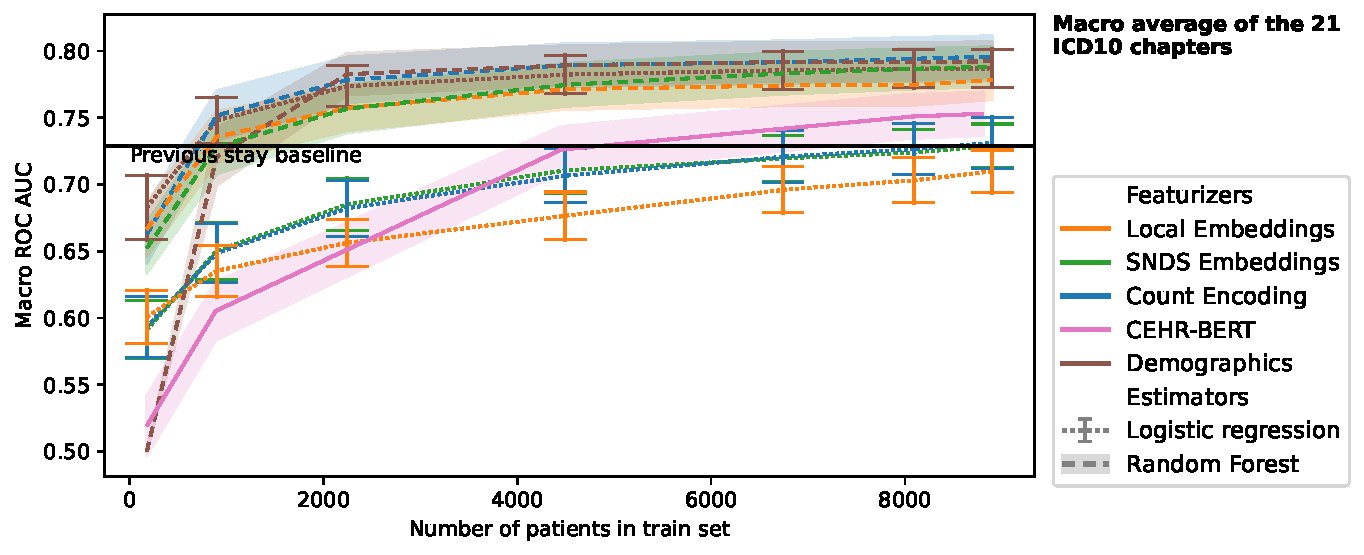
\includegraphics[width=0.8\linewidth]{img/chapter_3/prognosis/roc_auc_score__c_macro.pdf}
  \end{subfigure}
  \vfill
  \begin{subfigure}[b]{1\textwidth}
    \centering
    \caption{}\label{fig:prognosis_roc_auc_weighted}
    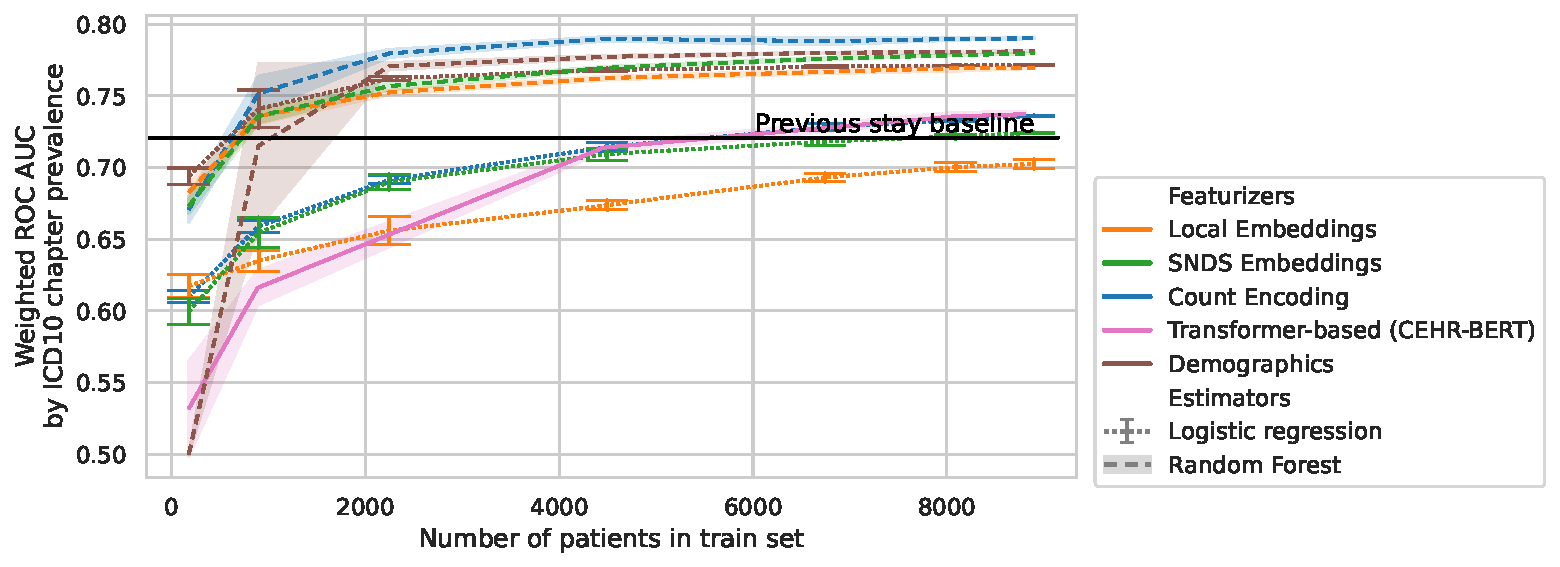
\includegraphics[width=0.8\linewidth]{img/chapter_3/prognosis/roc_auc_score__c_weighted.pdf}
  \end{subfigure}
  \caption{Prognosis ROC AUC average over chapters for different featurizers and
    estimators. The performances are averaged over 5 folds. The shaded area
    represents the standard deviation. The horizontal black lines display the
    naive baseline that predicts the previous stay codes for the target stay.
    Figure \ref{fig:prognosis_roc_auc_macro} averages all chapters with equal
    weight whereas \ref{fig:prognosis_roc_auc_weighted} averages chapters with
    their weight as prevalences. Random forest have better performances. Count
    encoder outperforms other featurizers, suggesting the importance of low
    count events that are smoothed out in embedding methods. Appendix
    \ref{apd:temporal_split:prognosis} details the results for each chapter and
    display Average Precision and Brier Score results.}%
  \label{fig:prognosis_roc_auc}
\end{figure}

Figure \ref{fig:prognosis_prevalences_auprc} shows the average precision score
performances for full effective train set and random forest estimators.
Performances increase with target prevalence. Appendix
\ref{apd:prognosis_prevalences} show similar results for ROC AUC and
linear estimators.


\begin{figure}[!h]
  \centering
  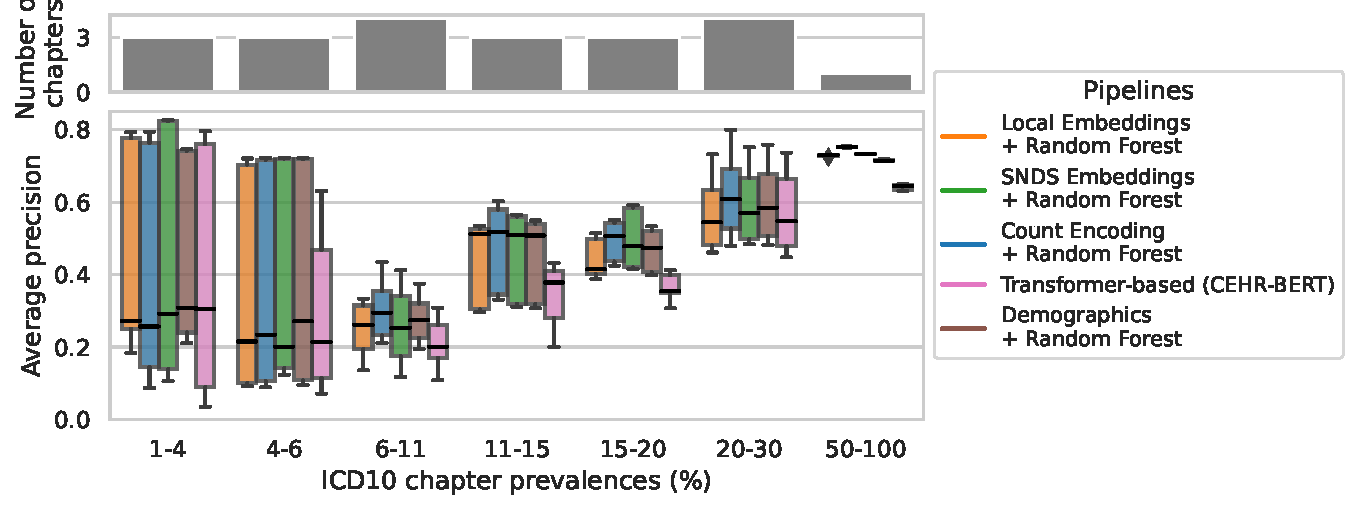
\includegraphics[width=0.8\linewidth]{img/chapter_3/prognosis/prevalence_results__est_random_forests_boxplot_average_precision_score_xlog.pdf}
  \caption{ Bigger target prevalences yield better average precision. The
    different chapters are binned in prevalence bins. The estimator used for
    this plot is random forest trained on the full effective train set. Appendix \ref{apd:prognosis_prevalences} details
    the ROC AUC curve.}%
  \label{fig:prognosis_prevalences_auprc}
\end{figure}

Figure \ref{fig:prognosis_training_time} shows the training time of the
different pipelines, highlighting the efficiency of the static embedding
methods.


\begin{figure}[!h]
  \centering
  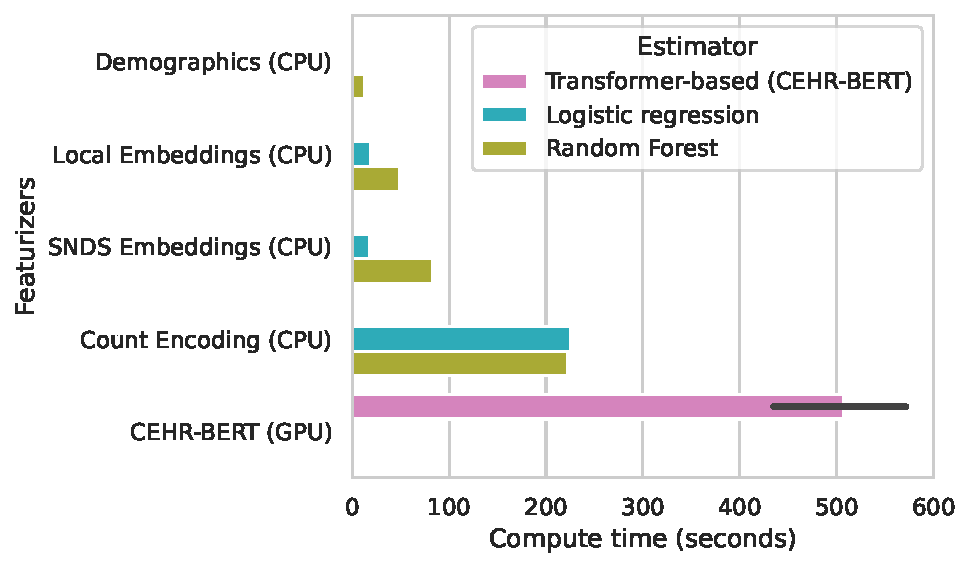
\includegraphics[width=0.8\linewidth]{img/chapter_3/prognosis/training_testing_time_per_chapter.pdf}
  \caption{Static embeddings are quicker to train. The training times are
    reported for the full train set for the prognosis task average on the 21
    ICD10 chapters. For all featurizers expect to CEHR-BERT, jobs were submitted
    with 10 CPU cores and 36GB memory on a slurm cluster. For CEHR-BERT, the
    calculation took place on the same cluster with a Nvidia T4 GPU with 16Gb of
    memory.}%
  \label{fig:prognosis_training_time}
\end{figure}


\paragraph{Static embeddings are quicker to train}%

Figure \ref{fig:prognosis_roc_auc} shows the training time of the different
pipelines for one chapter on the prognosis task.

% \begin{figure}
%   \centering
%   \includegraphics{img/chapter_3/training_times.pdf}
%   \caption{Training time for the different pipelines. The training time is
%     averaged over 5 folds for . The shaded area represents the standard deviation.
%     The training time for the transformer based model is significantly longer
%     than the other pipelines.}%
% \end{figure}


\section{Conclusion}\label{sec:predictive_models:conclusion}


% Restating the study
State-of-the-art predictive models from structured Electronic Medical Records
models are hindered by the unsolved challenge of publicly sharing pre-trained
models \citep{wornow2023shaky}. Training them from scratch requires important
computing resources, and access to very large cohorts. We explored the
complexity trade-off by studying different types of predictive algorithms, from
simple baseline to large scale transformers.


\paragraph{Simple problems are satured with simple models} The Long LOS
interpolation task is saturated by every model with close to 95\% ROC AUC.
Transferring static embeddings from a large external database allows to reach the
maximum performances with a small number of samples. For simple predictive tasks
such as administrative ones and small sample sizes, our results suggest that
using simple baselines based either on count encodings or static embeddings
followed by random forest is sufficient to reach good performances.

\paragraph{If concerned with training time, use static embedding pipelines}

The static embedding pipelines are faster to train than the count encoding and
transformer models. They show similar performances for most of the tasks and
medium sample size. They should be favored if it is necessary to frequently retrain the algorithm.

\paragraph{The prognosis task might not be a sound evaluation of predictive models}
Our experiments show that the prognosis task relies heavily on the previous stay
diagnoses codes and the patient demographics (age, sex, type of admission), with
only a small improvement of performances brought by the other type of features.
The inclusion of detailed events only matters for specific ICD10 chapters. This
highlights the importance of evaluating predictive models on clinically relevant
tasks aiming for inclusion in the healthcare workflow \citep{wornow2023shaky}.

\paragraph{Currently, we did not benchmark the MACE task}

MACE is more complicated to evaluate because of the low prevalence of the
outcome. This forced us to use a larger cohort to collect enough cases. Both
simple and complex models require large computing resources. However, the type
of theses resources are different. Static embeddings can reach satisfying
performances on big samples with large memory consumption (eg. 100GB of RAM).
Transformer architectures require large GPUs to be trained even for small sample
sizes. Because of constraints for these two types of resources on the AP-HP
computing cluster, we are currently not able to evaluate the MACE task on the
full cohort.

% limit
\paragraph{Further work} The high number of laboratory measurements for
hospitalized patients could improve the performances for all tasks. Due to
resource constraints, we did not include them into our features. For better
benchmarking with previous transformer-based models, a fourth task on heart
failure among type 2 diabetics should be explored. %

One argument in favor of recent large predictive models is their easy
repurposing for new sites and clinical tasks, requiring few labelled data.
However, there is currently little evidence of such successful transfers due to
difficult regulatory access to the pretrained model. Transferring between
hospitals and tasks in the APHP data warehouse would be a first step to evaluate this
claim.

%%%%%%%%%%%%%%%%%%%%%%%%%%%%%% CHAPTER 4 %%%%%%%%%%%%%%%%%%%%%%%%%%%%%%%%%%%%%%%
\chapter{Prediction is not all we need: Causal thinking for decision making on
  Electronic Health Records}\label{chapter:causal_tuto}

\begin{citationbox}
  All scientific work is incomplete - whether it be observational or
  experimental. All scientific work is liable to be upset or modified by
  advancing knowledge. That does not confer upon us a free- dom to ignore the
  knowledge we already have, or to postponethe action that it appears to demand
  at a given time.%

  \par\hfill --Austin Bradford Hill, \textit{The Environment and Disease: Association or Causation?}
\end{citationbox}

\begin{chapterabstract}\label{sec:causal_tuto:abstract}%
  While Chapter 3 focused on predictive models for patient outcomes, this
  chapter explores the causal framework to build clinically valuable models. It
  shows that predictions --even accurate as with machine learning, may not
  suffice to provide optimal healthcare for every patient. Indeed, prediction
  can be driven by shortcuts in the data, such as racial biases. Causal thinking
  is needed for data-driven decisions. Here, we give an introduction to the key
  elements, focusing on routinely-collected data, Electronic Health Records
  (EHRs) and claims data. Using such data to assess the value of an intervention
  requires care: temporal dependencies and existing practices easily confound
  the causal effect. We present a step-by-step framework to help build
  \emph{valid} decision making from real-life patient records by emulating a
  randomized trial before individualizing decisions, \emph{eg} with machine
  learning. Our framework highlights the most important pitfalls and
  considerations in analyzing EHRs or claims data to draw causal conclusions. We
  illustrate the various choices in studying the effect of albumin on sepsis
  mortality in the Medical Information Mart for Intensive Care database
  (MIMIC-IV). We study the impact of various choices at every step, from feature
  extraction to causal-estimator selection. In a tutorial spirit, the code and
  the data are openly available.
\end{chapterabstract}

\vfill
\begin{flushright}
  \begin{minipage}{15cm}
    {\small{This chapter corresponds to the article entitled \textit{Step-by-step
          causal analysis of Electronic Health Records to ground decision making}
        \underline{submitted} to \textit{npj Digital Medicine},}}\\

    {\small\hfill{} Authors: Matthieu Doutreligne, Tristan \textsc{Struja}, Judith
    \textsc{Abecassis}, Claire \textsc{Morgand}, Leo Anthony \textsc{Celi} and
    Gaël \textsc{Varoquaux}.}
  \end{minipage}
\end{flushright}

\clearpage
\minitoc

\section{Motivation : Healthcare is concerned with decision making, not mere
  prediction}%
\label{sec:causal_tuto:motivation}%

% \label{subsec:causal_tuto:predictive_medicine_biases}%
% \subsection{A key ingredient to ground data-driven decision making is causal thinking}%
% \label{subsec:causal_tuto:causal_thinking}%

% \subsection{The need for synthetic materials for practitioners}%
\label{subsec:causal_tuto:synthetic_materials}%


\paragraph{Medicine increasingly relies on data,} with the promise of better
clinical decision-making. Machine learning is central to this endeavor.
% Other formulation: "For such endeavor, machine learning is the darling
% of data scientists."
On medical images, it achieves human-level performance to
diagnose various conditions
\citep{aggarwal2021diagnostic,esteva2021deep,liu2019comparison}.
Using Electronic Health Records (EHRs) or administrative data, it
outperforms traditional rule-based clinical scores to predict a patient's
readmission risk, mortality, or future comorbidities
\citep{rajkomar2018scalable,li2020behrt,beaulieu2021machine}.
%
And yet, there is growing evidence that machine-learning models may not benefit
patients equally. They reproduce and amplify biases in the data
\citep{rajkomar2018ensuring}, such as gender or racial biases
\citep{singh2022generalizability,gichoya2022ai,roosli2022peeking},
or marginalization of under-served populations
\citep{seyyed2021underdiagnosis}. The models
typically encode these biases by capturing shortcuts: stereotypical features in the data or inequal sampling \citep{geirhos2020shortcut,winkler2019association,degrave2021ai}.
%
For instance, an excellent predictive model of mortality in the Intense Care Unit
(ICU) might be of poor clinical value if it uses information available
only too late.
%
These shortcuts are at odds with healthcare's ultimate goal: appropriate care
for optimal health outcome for each and every patient
\citep{cma_policy_appropriateness_2015, ghassemi2020review}. Making the right decisions requires more than accurate predictions.

\paragraph{Causal thinking} is a key ingredient to ground data-driven decision making \citep{prosperi2020causal}. Indeed, decision-making logic cannot rely purely on
learning from the data, which itself results from a history of prior
decisions \citep{plecko2022causal}. Rather, reasoning about a putative
intervention requires comparing the potential outcomes with and without the
intervention, the difference between these being the causal
effect.
% TODO: reintroduce counterfactual predictions? Not sure, given that it
% does not fit well with the rest of our manuscript
In medicine, causal effects
are typically measured by Randomized Control Trials
(RCTs).
Yet, RCTs may not suffice for individualized decision making: They
may suffer from selection biases \citep{travers2007external,
  averitt2020translating}, failure to recruit disadvantaged groups, and
become outdated by evolving clinical practice. Their limited sample size
seldom allows to explore treatment heterogeneity across subgroups.
%
Rather, routinely-collected data naturally probes real-world practice and
displays much less sampling bias. It provides a unique opportunity to assess benefit-risk
trade-offs associated with a decision \citep{desai2021broadening}, with
sufficient data to capture heterogeneity \citep{rekkas2023standardized}.
Estimating causal effects from this data is challenging however,
as the intervention is far from being given at random, and,
as a result, treated and untreated patients cannot be easily compared. Without
dedicated efforts, machine-learning models simply pick up these difference and
are not usable for decision making. Rather dedicated statistical
techniques are needed to emulate a ``target trial'' from \emph{observational} data
-- without controlled interventions.

\paragraph{Different time resolutions} EHRs and claims are two prominent sources of real-life healthcare data with different time resolutions.
EHRs are particularly suited to guide clinical decisions, as they are
rich in high-resolution and time-varying features, including vital signs,
laboratory tests, medication dosages, etc. Claims, on the other
hand, inform best on medico-economic questions or
chronic conditions as they cover in-patient and
out-patient care during extended time periods.
%
But there are many pitfalls to sound and valid
causal inferences \citep{hernan2019second, schneeweiss2021conducting}.
%
Data with temporal dependencies, as EHRs and claims, are particularly
tricky, as it is easy to induce time-related biases
\citep{suissa2008immortal,wang2023emulation}.

% Position of our paper
\paragraph{Objectives and structure of the chapter} Here we summarize the main
considerations to derive valid decision-making evidence from EHRs and claims
data.
%
Many guidelines on causal inference from observational data have been
written in various
fields such as epidemiology \citep{hernan2020causal, schneeweiss2021conducting,
  zeng2022uncovering}, statistics \citep{belloni2014high,
  chernozhukov2018double}, machine learning \citep{shalit2016tutorial,
  sharma2018tutorial,moraffah2021causal} or econometrics \citep{imbens2009recent}.
Time-varying features of EHR data, however, raise particular challenges that call
for an adapted framework.
%
We focus on single interventions: only one prescription during the study period,
e.g., a patient either receives mechanical ventilation or not during admission to an
intensive care unit compared to, e.g. blood transfusion which may be given repeatedly.
%
Section \ref{sec:causal_tuto:framework} details our proposed step-by-step
analytic framework on EHR data. Section \ref{sec:causal_tuto:application}
instantiates the framework by emulating a trial on the effect of albumin on
sepsis using the Medical Information Mart for Intensive Care database (MIMIC-IV)
database \citep{johnson2020mimic}. Section \ref{subsec:causal_tuto:discussion}
discusses our results and its implications on sound decision making. These
sections focus on being accessible, appendices and online Python
code\footnote{\url{https://github.com/soda-inria/causal_ehr_mimic/}} expand more
technical details, keeping a didactic flavor.



\section{Step-by-step framework for robust decision making from EHR data}%
\label{sec:causal_tuto:framework}%


% motivating example
\paragraph{The need for a causal framework, even with machine learning}\label{causal_tuto:motivating_example}

Data analysis without causal framing risks building shortcuts. As an example of
such failure, we trained a predictive model for 28-day mortality in patients
with sepsis within the ICU. We fit the model using clinical measures available
during the first 24 hours after admission. To simulate using this model to decide
whether or not to administrate resuscitation fluids, we evaluate its performance
on unseen patients first on the same measures as the ones used in training, and then using only the measures available before this treatment, as would be done in a decision making context. The
performance drops markedly: from 0.80 with all the measures available during the first 24 hours after admission to 0.75 using only the measures available before the treatment (unit: Area Under the Curve of the Receiving Operator Characteristic, ROC AUC).
The model has captured shortcuts: good prediction based on the wrong features of the
data, useless for decision making.
On the opposite, a model trained on pre-treatment measures achieves 0.79 in
the decision-making setting (further details
in appendix \ref{apd:motivating_example}). This illustrates the importance of
accounting for the putative interventions even for predictive models.

Whether a data analysis uses machine learning or not, many pitfalls
threaten its value for decision making. To avoid these traps,
we outline in this section a simple step-by-step analytic framework,
illustrated in Figure \ref{fig:inference_framework}. We first study the medical
question as a target trial \citep{hernan2021methods}, the common
evidence for decisions. This enables assessing the validity of the
analysis before probing heterogeneity --predictions on sub-groups-- for
individualized decision.

\begin{figure}[!t]
  \centering
  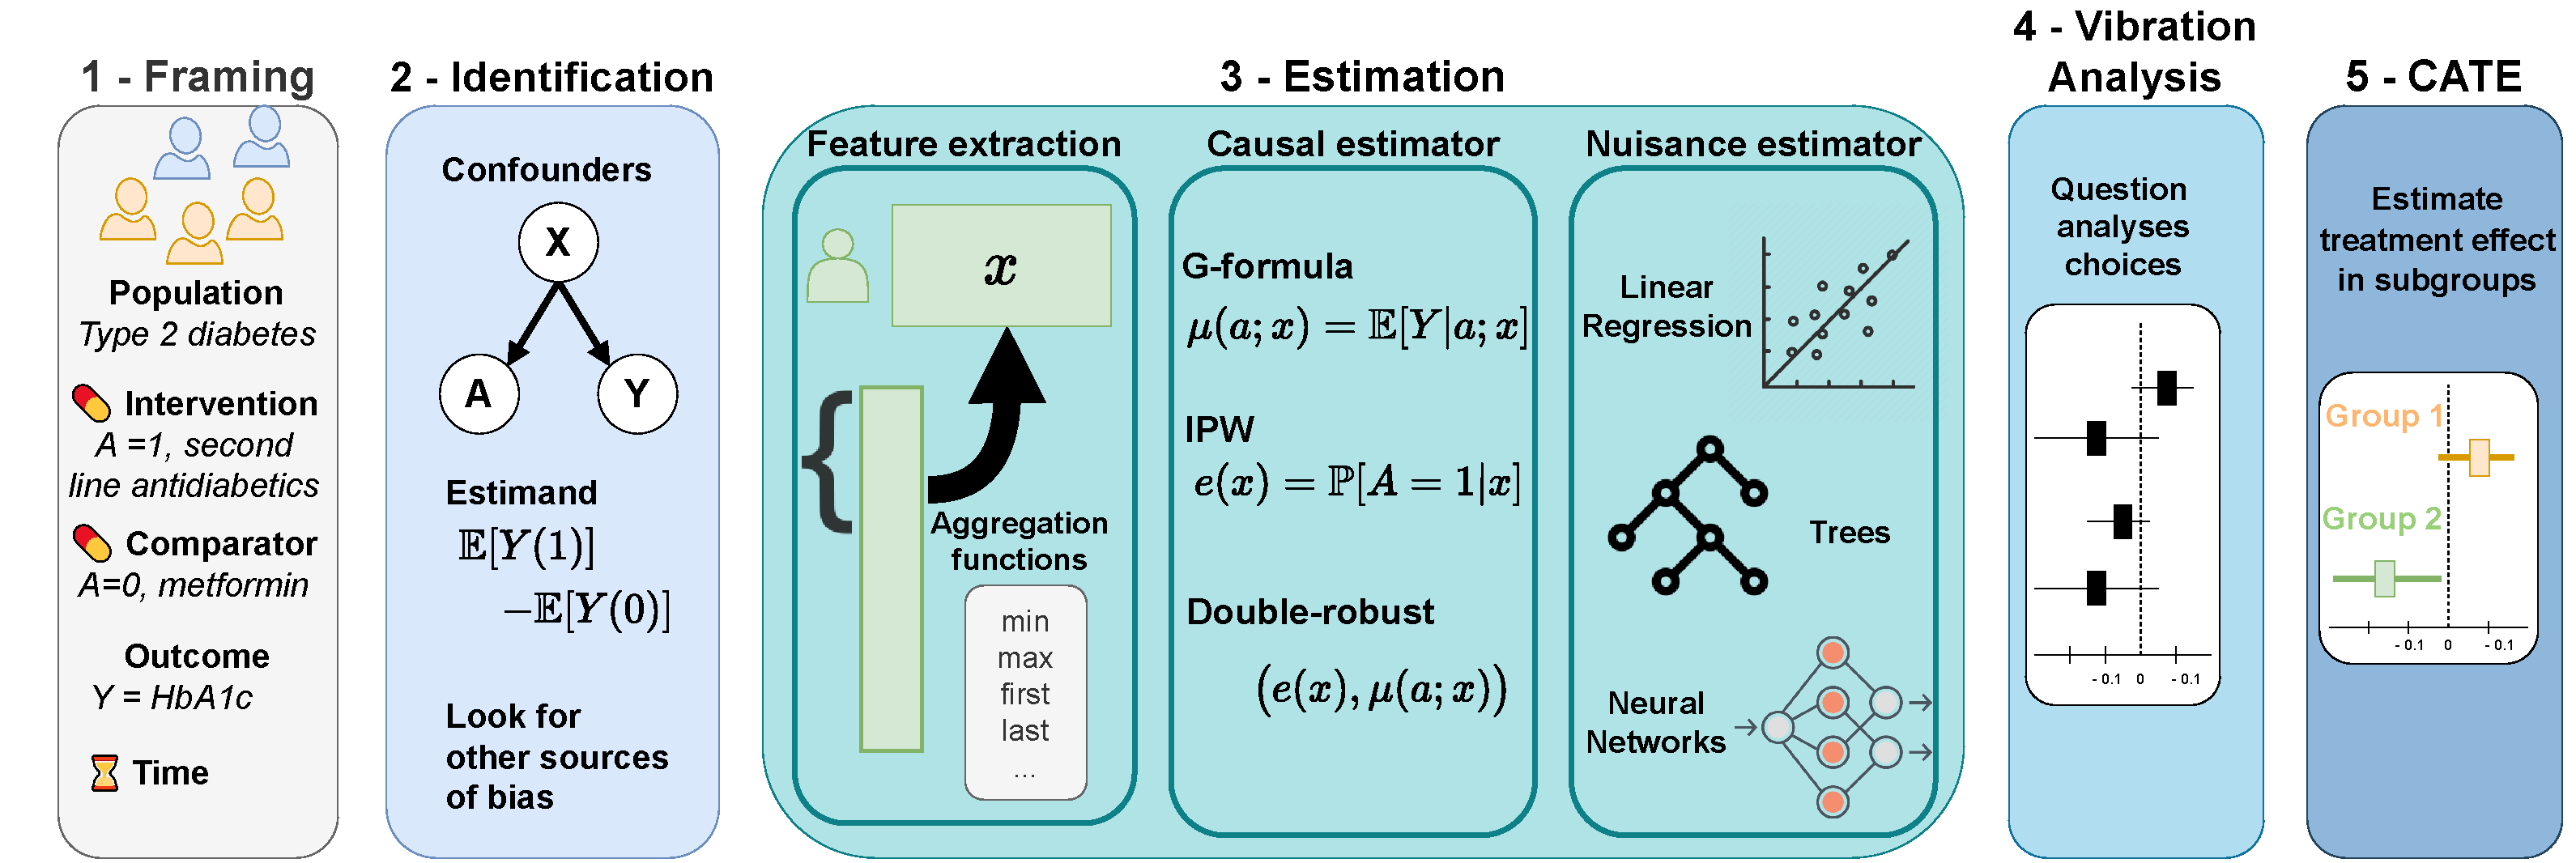
\includegraphics[width=1.0\linewidth]{img/chapter_4/complete_inference_flow.pdf}
  \caption{\textbf{Step-by-step analytic framework} -- The complete
    inference pipeline confronts the analyst with
    many choices, some guided by domain knowledge, others
    by data insights. Making those choices explicit is necessary to ensure
    robustness and reproducibility.}\label{fig:inference_framework}
\end{figure}

\subsection{Step 1: study design -- Frame the question to avoid biases}%
\label{subsec:causal_tuto:framing}%

\begin{table}[b!]
  \resizebox{\textwidth}{!}{%
    \begin{tabular}{|l|l|l|l|}
      \hline
      \multicolumn{1}{|c|}{\textbf{PICO component}} &
      \multicolumn{1}{c|}{\textbf{Description}}     &
      \multicolumn{1}{c|}{\textbf{Notation}}        &
      \multicolumn{1}{c|}{\textbf{Example}}                                                            \\ \hline
      \textbf{\textcolor{P}{Population}}            & \makecell[l]{What is the target                  \\population of interest?}
                                                    & $X \sim \mathbb{P}(X)$,
      the covariate distribution                    &
      \makecell[l]{Patients with sepsis in the ICU}                                                    \\ \hline
      \textbf{\textcolor{I}{Intervention}}          &
      What is the treatment?                        &
      \makecell[l]{$A \sim \mathbb{P}(A=1)=p_A$,                                                       \\ the probability to be treated} &
      \makecell[l]{Crystalloids and albumin                                                            \\ combination}                                                          \\ \hline
      \textbf{\textcolor{C}{Control}}               & \makecell[l]{What is the clinically              \\ relevant comparator?}
                                                    & $1-A \sim 1-p_A$                               &
      Crystalloids only
      \\ \hline
      \textbf{\textcolor{O}{Outcome}}               & \makecell[l]{What are the
      outcomes ?}                                   & \makecell[l]{$Y(1), Y(0) \sim \mathbb{P}(Y(1),
      Y(0))$,                                                                                          \\ the
      potential outcomes distribution}              & 28-day mortality
      \\ \hline

      \textbf{\textcolor{T}{Time}}                  & \makecell[l]{Is the start
        of follow-up aligned
      \\with intervention assignment?} & \makecell[l]{N/A}
                                                    & \makecell[l]{Intervention administered within
      \\  the first
      24 hours of admission}                                                                           \\ \hline
    \end{tabular}%
  }\\
  \caption{PICO(T) components help to clearly define the
    medical question of interest.}\label{table:picot}
\end{table}


\begin{figure}[b!]
  %  \begin{minipage}{.2\linewidth}
  % \end{minipage}%
  % \hfill%
  % \begin{minipage}{.78\linewidth}
  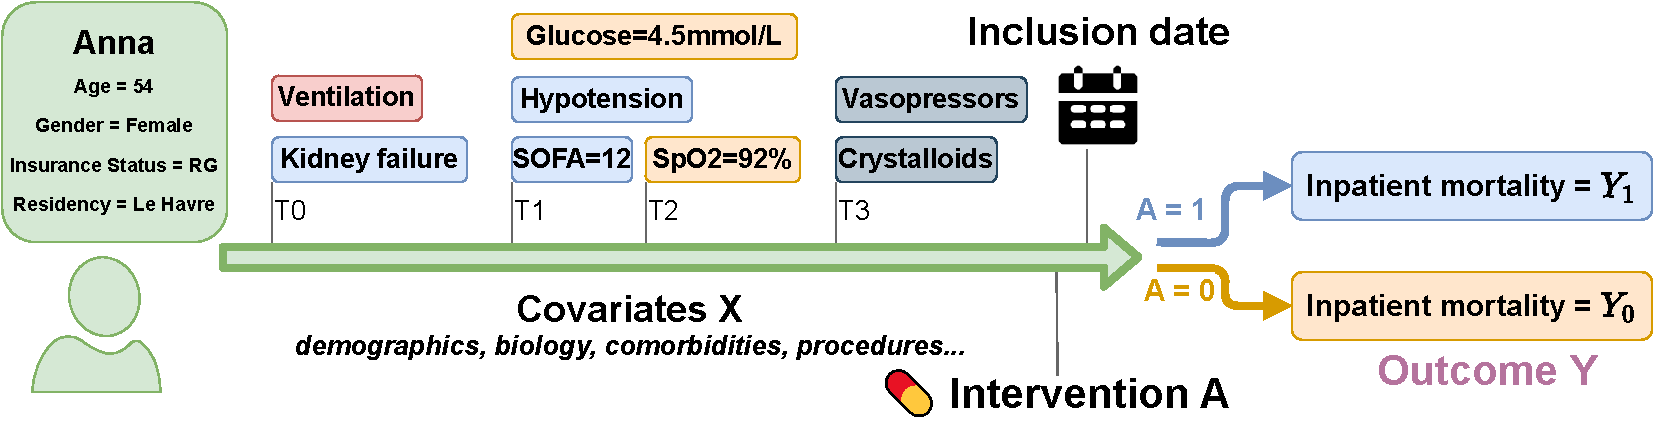
\includegraphics[width=\linewidth]{img/chapter_4/counterfactual_event_format.pdf}
  \caption{\textbf{Study design} -- The first step of the analysis consists in identifying a valid
    treatment effect question from patient healthcare trajectories and defining
    a target trial emulating a RCT using the PICO(T) framework.}\label{fig:counterfactual_event_format}
  %\end{minipage}%
\end{figure}


\paragraph{PICO(T) format} Grounding decisions on evidence needs well-framed questions, defined by
their PICO components: Population, Intervention, Control, and Outcome
\citep{richardson1995well}. To concord with a (hypothetical)
target randomized clinical trial, an analysis must emulate all these components
\citep{hernan_using_2016,wang2023emulation}, \emph{eg} via
\emph{potential outcome} statistical framework \citep{hernan2020causal}
--Table \ref{table:picot} and Figure \ref{fig:counterfactual_event_format}.
EHRs and Claims need an additional time component: PICOT \citep{riva2012your}.

Without dedicated care, defining those PICO(T) components from EHRs can
pick up bias: non-causal associations between treatment and outcomes.
We detail two common sources of bias in the
Population and Time components: selection bias and immortal time bias, respectively.

\paragraph{Selection Bias:} In EHRs, outcomes and treatments are often not
directly available and need to be inferred from indirect events. These signals
could be missing not-at random, sometimes correlated with the treatment
allocation \citep{weiskopf2023healthcare}. For example, not all billing
codes are equally well filled in, as billing is strongly associated with
case-severity and cost.
Consider comparing the effect on mortality of fluid resuscitation
with albumin to that of crystalloids. As albumin is much more costly,
patients who have received this treatment are much more likely to have
a sepsis billing code, independent of the seriousness of their
condition. On the contrary, for patients treated with crystalloids, only
the most severe cases will have a billing code. Naively comparing patients on crystalloid treatment with
less sick patients on albumin treatment would overestimate the effect of albumin.

\paragraph{Immortal time bias:} Another common bias comes from timing:
improper alignment of the inclusion defining event and the intervention time
\citep{suissa2008immortal,hernan2016specifying,wang2022understanding}. Figure
\ref{fig:immortal_time_bias} illustrates this
Immortal time bias --related to survivor bias \citep{lee2020immortaltimebias}.
It occurs when the follow-up period, i.e. cohort entry, starts before the
intervention, e.g. prescription for a
second-line treatment. In this case, the treated group will be
biased towards patients still alive at the time of assignment and thus
overestimating the effect size. Other common temporal biases are lead time bias
\citep{Oke2021leadtimebias,fu2021timing}, right censorship
\citep{hernan2016specifying}, and attrition bias
\citep{Bankhead2017attritionbias}.


Good practices include explicitly stating the cohort inclusion event
\citep[Chapter~10:Defining Cohorts]{ohdsi2019book} and defining an appropriate
grace period between starting time and the intervention assignment
\citep{hernan2016specifying}. At this step, a population timeline can help (eg.
Figure \ref{fig:cohort_timeline_albumin}).

\begin{figure}[!h]
  \begin{minipage}{.25\linewidth}
    \caption{Poor experimental design can introduce Immortal time bias, which
      leads to a treated group with falsely longer longevity
      \citep{lee2020immortaltimebias}.}\label{fig:immortal_time_bias}
  \end{minipage}%
  \hfill%
  \begin{minipage}{.7\linewidth}
    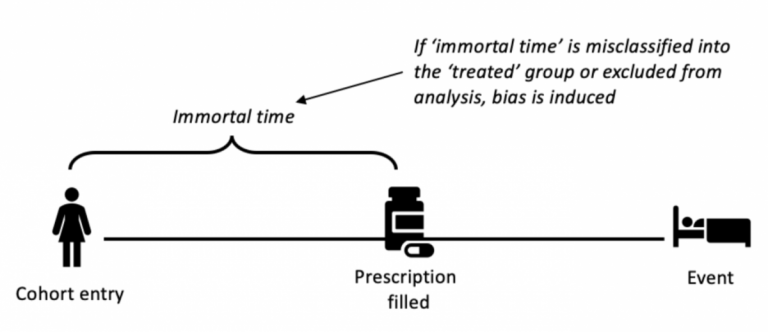
\includegraphics[width=\linewidth]{img/chapter_4/catalog_of_bias_immortal_time_bias.png}
  \end{minipage}
\end{figure}


\subsection{Step 2: identification -- List necessary information to answer the causal question}%
\label{subsec:causal_tuto:identification}%


The identification step builds a causal model to answer the research question
(Figure \ref{fig:causal_diagram_albumin}).
%
Indeed, the analysis must compensate for differences between treated and
non-treated that are not due to the intervention
(\cite[chapter~1]{pearl2018book}, \cite[chapter~1]{hernan2020causal}).

\begin{background_box_left}

  \paragraph{Causal Assumptions}\label{background:causal_assumptions}

  Not every question can be answered from a given dataset: valid causal
  inference requires assumptions. We assume the following four assumptions,
  referred as strong ignorability and necessary to assure identifiability of the
  causal estimands with observational data \citep{rubin_causal_2005}. See
  \cite{naimi2023defining} for a concise introduction for epidemiologists:

  \begin{assumption}[Unconfoundedness]\label{assumption:ignorability}
    \begin{equation*}\label{eq:ignorability}
      \{Y(0), Y(1) \} \indep A | X
    \end{equation*}
    This condition --also called ignorability-- is equivalent to the conditional
    independence on $e(X)$ \citep{rosenbaum_central_1983}: $\{Y(0), Y(1) \}
      \indep  A | e(X)$.
  \end{assumption}


  \begin{assumption}[Overlap, also known as Positivity)]\label{assumption:overlap}
    \begin{equation*}\label{eq:overlap}
      \eta < e(x) < 1 - \eta \quad \forall x \in \mathcal X \text{ and some } \eta > 0
    \end{equation*}
    The treatment is not perfectly predictable. Or with different words, every
    patient has a chance to be treated and not to be treated. For a given set of
    covariates, we need examples of both to recover the ATE.
  \end{assumption}

  As noted by \cite{damour_overlap_2020}, the choice of covariates $X$ can
  be viewed as a trade-off between these two central assumptions. A bigger
  covariates set generally reinforces the ignorability assumption. In the
  contrary, overlap can be weakened by large $\mathcal{X}$ because of the
  potential inclusion of instruments: variables only linked to the treatment which
  could lead to arbitrarily small propensity scores.

  % remark: There is a major counter example to these colliders (variables which
  % are caused by both the outcome and the treatment),

  \begin{assumption}[Consistency]\label{assumption:consistency} The observed
    outcome is the potential outcome of the assigned treatment:
    \begin{equation*}\label{eq:consistancy}
      Y = A \, Y(1) + (1-A) \, Y(0)
    \end{equation*}
    Here, we assume that the intervention $A$ has been well defined. This
    assumption focuses on the design of the experiment. It clearly states the link
    between the observed outcome and the potential outcomes through the
    intervention \citep{hernan_causal_2020}.
  \end{assumption}

  \begin{assumption}[Generalization]\label{assumption:generalization} The training
    data on which we build the estimator and the test data on which we make the
    estimation are drawn from the same distribution $\mathcal D^*$, also known as
    the ``no covariate shift'' assumption \citep{jesson_identifying_2020}.
  \end{assumption}


  \paragraph{Categorizing covariates}
  %
  Potential predictors --covariates-- should be categorized depending on their
  causal relations with the intervention and the outcome (Figure
  \ref{fig:causal_variables}): \emph{confounders} are common causes of the
  intervention and the outcome; \emph{colliders} are caused by both the
  intervention and the outcome; \emph{instrumental variables} are a cause of the
  intervention but not the outcome, \emph{mediators} are caused by the
  intervention and is a cause of the outcome. Finally, \emph{effect modifiers}
  interact with the treatment, and thus
  modulate the treatment effect in subpopulations \citep{attia2022proposal}.

\end{background_box_left}

\begin{figure}
  \begin{minipage}[t]{0.18\linewidth}
    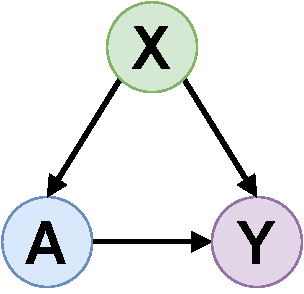
\includegraphics[width=0.72\linewidth]{img/chapter_4/confounder.pdf}

    \small\sffamily Confounder
  \end{minipage}
  \hfill
  \begin{minipage}[t]{0.18\linewidth}
    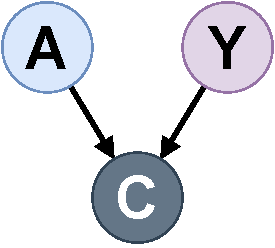
\includegraphics[width=0.72\linewidth]{img/chapter_4/collider.pdf}

    \small\sffamily Collider
  \end{minipage}
  \hfill
  \begin{minipage}[t]{0.18\linewidth}
    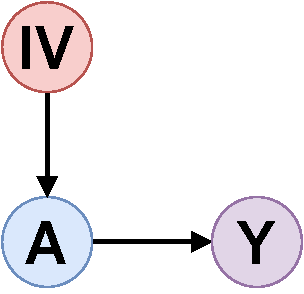
\includegraphics[width=0.72\linewidth]{img/chapter_4/instrumental_variable.pdf}

    \small\sffamily Instrumental variable
  \end{minipage}
  \hfill
  \begin{minipage}[t]{0.18\linewidth}
    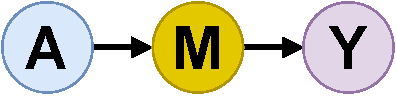
\includegraphics[width=.9\linewidth]{img/chapter_4/mediator.pdf}%

    \small\sffamily Mediator
  \end{minipage}
  \hfill
  \begin{minipage}[t]{0.18\linewidth}
    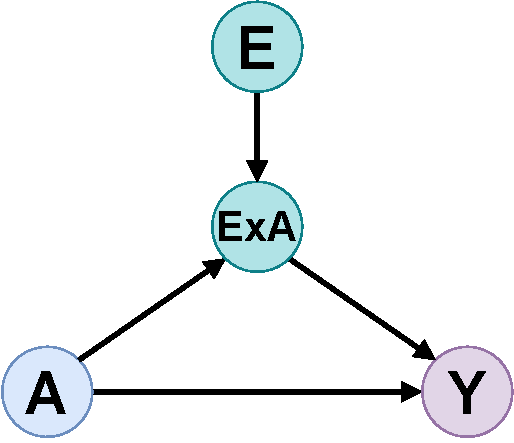
\includegraphics[width=\linewidth]{img/chapter_4/effect_modifier.pdf}%
    \llap{%
      \raisebox{.555\linewidth}{\colorbox{black!10}{\parbox{1.9\linewidth}{%
            \sffamily\small\hspace*{-1.3ex}%
            \begin{tabular}{r@{\hskip 1ex}lr@{\hskip 1ex}l}
              A:  & Treatment                    & Y: & Outcome         \\
              X:  & Confounder                   & C: & Collider        \\
              IV: & Instrumental va\rlap{riable}                        \\
              M:  & Mediator                     & E: & Effect modifier \\
            \end{tabular}%
            \vspace*{-.3ex}
          }}\hspace*{.84\linewidth}%
      }}

    \small\sffamily Effect modifier \scriptsize\\\citep[Represented
      following][]{attia2022proposal}
  \end{minipage}
  \caption{The five categories of causal variables needed for our
    framework.}\label{fig:causal_variables}
\end{figure}

\begin{background_box_left}

  To capture a valid causal effect, the analysis should only include confounders
  and possible treatment-effect modifiers to study the resulting heterogeneity.
  Regressing the outcome on instrumental and post-treatment variables (colliders
  and mediators) will lead to biased causal estimates
  \citep{vanderweele2019principles}. Drawing causal Directed Acyclic Graphs (DAGs)
  \citep{greenland1999causal}, \emph{eg} with a webtool such as DAGitty
  \citep{textor2011dagitty}, helps capturing the relevant variables from domain
  expertise.

  \paragraph{Estimand or effect measure}

  The \emph{estimand} is the final statistical quantity estimated from the data.
  %
  Depending on the question, different estimands are better suited to contrast the
  two potential outcomes E[Y(1)] and E[Y(0)] \citep{imbens_nonparametric_2004,
    colnet2023risk}. For continuous outcomes, risk difference is a natural estimand,
  while for binary outcomes (e.g. events)  the choice of estimand depends on the
  scale of the study. Whereas the risk difference is very informative at the
  population level, e.g. for medico-economic decision making, the risk ratio and
  the hazard ratio are more informative to reason on sub-populations such as
  individuals or sub-groups \citep{colnet2023risk}.

\end{background_box_left}

\subsection{Step 3: Estimation -- Compute the causal effect of interest}\label{subsec:causal_tuto:estimation}

\paragraph{Confounder aggregation}

Some confounders are captured via measures collected over multiple time points.
These need to be aggregated at the patient level. Simple forms of aggregation
include taking the first or last value before a time point, or an aggregate such
as mean or median over time. More elaborate choices may rely on hourly
aggregations of information such as vital signs. These provide more detailed
information on the health evolution, thus reducing confounding bias between
rapidly deteriorating and stable patients. However, it also increases the number
of confounders, resulting in a larger covariate space, hence increasing the
estimate's variance and endangering the positivity assumption. The choices
should be guided by expert knowledge. If multiple choices appear reasonable, one
should compare them in a vibration analysis (see Section
\ref{subsec:causal_tuto:vibration_analysis}). Indeed, aggregation may impact results, as
\cite{sofrygin2019targeted} show, revealing that some choices of averaging time
scale lead to inconclusive links between HbA1c levels and survival in diabetes.

Beyond measures and clinical codes, unstructured clinical text may capture
confounding or prognostic information \citep{horng2017creating,jiang2023health}
which can be added in the causal model \citep{zeng2022uncovering}.

\paragraph{Causal estimators or statistical modeling}

A given estimand can be estimated through different methods. One can model the
outcome with regression models \citep[also known as
  G-formula,][]{robins_role_1986} and use it as a predictive counterfactual model
for all possible treatments for a given patient. Alternatively, one can model
the propensity of being treated use it for matching or Inverse Propensity
Weighting (IPW) \citep{austin2015moving}. Finally, doubly robust methods model
both the outcome and the treatment, benefiting from the convergence of both
models \citep{wager2020stats}. Various doubly robust models have emerged:
Augmented Inverse Propensity Score (AIPW) \citep{robins1994estimation}, Double
Robust Machine Learning \citep{chernozhukov2018double}, or Targeted Maximum
Likelihood Estimation (TMLE) \citep{schuler2017targeted} to name a few. We
detail their statistical properties in Appendix \ref{apd:causal_estimators},
giving some hints on when to choose one method over the others.

\paragraph{Estimation models of outcome and treatment}

The causal estimators use models of the outcome or the treatment --called
nuisances as they are not the main inference targets in our causal effect
estimation problem. Which statistical model is best suited is an additional
choice and there is currently no clear best practice
\citep{wendling2018comparing, dorie2019automated}. The trade-off lies between
simple models risking misspecification of the nuisance parameters versus
flexible models risking to overfit the data at small sample sizes. Stacking
models of different complexity in a super-learner is a good solution to navigate
the trade-off \citep{van2007super,doutreligne2023select}.

\subsection{Step 4: Vibration analysis -- Assess the robustness of the hypotheses}
\label{subsec:causal_tuto:vibration_analysis}%

Some choices in the pipeline may not be clear cut. Several options should then
be explored, to derive conceptual error bars going beyond a single statistical
model. This process is sometimes called robustness analysis
\citep{neumayer2017robustness} or sensitivity analysis
\citep{thabane2013tutorial, hernan2020causal,fda_statistical_2021}. However, in
epidemiology, sensitivity analysis refers to quantifying the bias from
unobserved confounders \citep{schneeweiss2006sensitivity}. Following
\cite{patel2015assessment}, we use the term vibration analysis to describe the
sensitivity of the results to all analytic choices.
%
The vibration analysis can identify analytic choices that deserve extra
scrutiny. It complements a comparison to previous studies --ideally RCTs-- to
establish the validity of the pipeline.



\subsection{Step 5: Treatment heterogeneity -- Compute treatment effects on subpopulations}%
\label{subsec:causal_tuto:heterogeneity}%


Once the causal design and corresponding estimators are established, they can be
used to explore the variation of treatment effects among subgroups. Measures of
the heterogeneity of a treatment nourish decisions tailored to a patient's
characteristics. A causally-grounded model, \emph{eg} using machine learning,
can be used to predict the effect of the treatment from all the covariates
--confounders and effect modifiers-- for an individual: the \emph{Individual
  Treatment Effect} \citep[ITE][]{lu2018estimating}. Studying heterogeneity only
along specific covariates, or a given patient stratification, is related to the
\emph{Conditional Average Treatment Effect} (CATE)
\citep{robertson2021assessing}. Practically, CATEs can be estimated by
regressing the individual predictions given by the causal estimator against the
sources of heterogeneity (details in \ref{apd:cate_results}).


\section{Application: evidence from MIMIC-IV on which resuscitation fluid to
  use}%
\label{sec:causal_tuto:application}%

We now use the above framework to extract evidence-based decision
rules for resuscitation.
Ensuring optimal organ perfusion in patients with septic shock requires
resuscitation by reestablishing circulatory volume with intravenous fluids.
While crystalloids are readily available, inexpensive and safe, a large fraction
of the administered volume is not retained in the vasculature. Colloids
offer the theoretical benefit of retaining more volume in the circulation, but
might be more costly and have adverse effects \citep{annane2013effects}. The
scientific community long debated which fluid benefits patients most
\citep{mandel2023treatment}.

\paragraph{Emulated trial: Effect of albumin in combination with crystalloids
  compared to crystalloids alone on 28-day mortality in patients with sepsis}\label{emulated_trial}

We illustrate the impact of the different analytical steps to conclude
on the effect of albumin in combination with crystalloids compared to
crystalloids alone on 28-day mortality in patients with sepsis using MIMIC-IV
\citep{johnson2020mimic}. This question is clinically relevant and
multiple published RCTs
can validate the average treatment effect.
Appendix \ref{apd:target_trials} provides further examples of
potential target trials.


\paragraph{Evidence from the literature}

Meta-analyses from multiple pivotal RCTs
found no effect of adding albumin to crystalloids \citep{li2020resuscitation} on
28-day and 90-day mortality. Further, an observational study in MIMIC-IV
\citep{zhou2021early} found no significant benefit of albumin on 90-day
mortality for severe sepsis patients. Given this previous evidence, we thus expect
no average effect of albumin on mortality in sepsis patients. However,
studies --RCT \citep{caironi2014albumin} and observational
\citep{li2020resuscitation}-- have found that septic-shock
patients do benefit from albumin.

\subsection{Study design: effect of crystalloids on mortality in sepsis}%
\label{subsec:causal_tuto:framing_mimic}%


\begin{itemize}[leftmargin=2ex]
  \item \textcolor{P}{Population}: Patients with sepsis within the ICU stay
        according to the sepsis-3 definition. Other inclusion criteria:
        sufficient follow-up of at least 24 hours, and age over 18 years
        described in table \ref{table:albumin_for_sepsis:table1_simple}.

  \item \textcolor{I}{Intervention}: Treatment with a combination of
        crystalloids and albumin during the first 24 hours of an ICU stay.

  \item \textcolor{C}{Control}: Treatment with crystalloids only in the first 24
        hours of an ICU stay.

  \item \textcolor{O}{Outcome}: 28-day mortality.

  \item \textcolor{T}{Time}: Follow-up begins after the first administration of
        crystalloids. Thus, we potentially introduce a small immortal time bias
        by allowing a time gap between follow-up and the start of the albumin
        treatment --shown in Figure \ref{fig:cohort_timeline_albumin}. Because
        we are only considering the first 24 hours of an ICU stay, we
        hypothesize that this gap is insufficient to affect our results. We test
        this hypothesis in the vibration analysis step
        \ref{subsec:causal_tuto:vibration_mimic}.
\end{itemize}


\begin{figure}[h!]
  \centering
  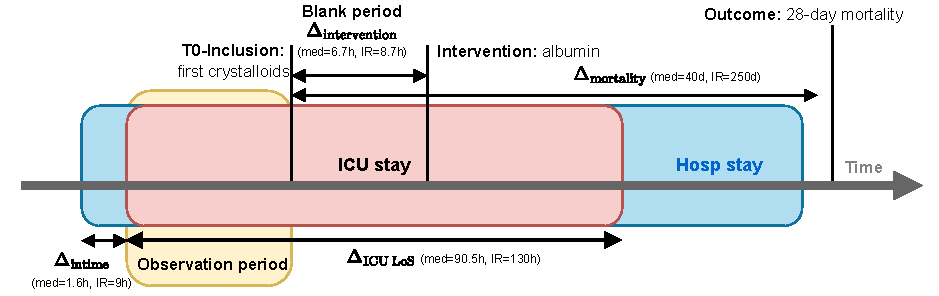
\includegraphics[width=\linewidth]{img/chapter_4/timeline_albumin_for_sepsis.pdf}
  \caption{Defining the inclusion event, the starting time T0 for follow-up, the
    intervention's assignment time and the observation window for confounders is
    crucial to avoid time and selection biases. In our study, the gap
    between the intervention and the inclusion is small
    compared to the occurrence of the outcome to limit immortal time bias: 6.7 hours vs 40
    days for mortality.\label{fig:cohort_timeline_albumin}}
\end{figure}


In MIMIC-IV, these inclusion criteria yield 18,121 patients with 3,559 patients
treated with a combination of crystalloids and albumin (Appendix
\ref{apd:selection_flowchart} details the selection flowchart).


\subsection{Identification: listing confounders}%
\label{subsec:causal_tuto:confounders_mimic}%

We enrich the confounders selection procedure described by \cite{zhou2021early}
with expert knowledge, creating the causal DAG shown in Figure
\ref{fig:causal_diagram_albumin}. Gray confounders are not controlled for, since
they are not available in the data. However, resulting confounding biases are
captured by proxies such as comorbidity scores (SOFA or SAPS II) or other
variables (eg. race, gender, age, weight).
%
Appendix \ref{apd:albumin_for_sepsis:table1_complete} details confounders
summary statistics for treated and controls.


\begin{table*}[!tb]
  \resizebox*{\textwidth}{!}{
    %\centering%\small
    \begin{tabular}{llllll}
\toprule
{} & Missing &       Overall & Cristalloids only & Cristalloids + Albumin & P-Value \\
                           &         &               &                   &                        &         \\
\midrule
n                          &         &         18421 &             14862 &                   3559 &         \\
Female, n (\%)              &         &   7653 (41.5) &       6322 (42.5) &            1331 (37.4) &         \\
White, n (\%)               &         &  12366 (67.1) &       9808 (66.0) &            2558 (71.9) &         \\
Emergency admission, n (\%) &         &   9605 (52.1) &       8512 (57.3) &            1093 (30.7) &         \\
admission\_age, mean (SD)   &       0 &   66.3 (16.2) &       66.1 (16.8) &            67.3 (13.1) &  <0.001 \\
SOFA, mean (SD)            &       0 &     6.0 (3.5) &         5.7 (3.4) &              6.9 (3.6) &  <0.001 \\
lactate, mean (SD)         &    4616 &     3.0 (2.5) &         2.8 (2.4) &              3.7 (2.6) &  <0.001 \\
\bottomrule
\end{tabular}
%
    %\\[.5ex]
  }
  \caption{Characteristics of the trial population measured on the first 24
    hours of ICU stay. Appendix \ref{apd:table:albumin_for_sepsis:table1_complete}
    describes all confounders used in the analysis.}\label{table:albumin_for_sepsis:table1_simple}
\end{table*}


\begin{figure}[t!]
  \centering%
  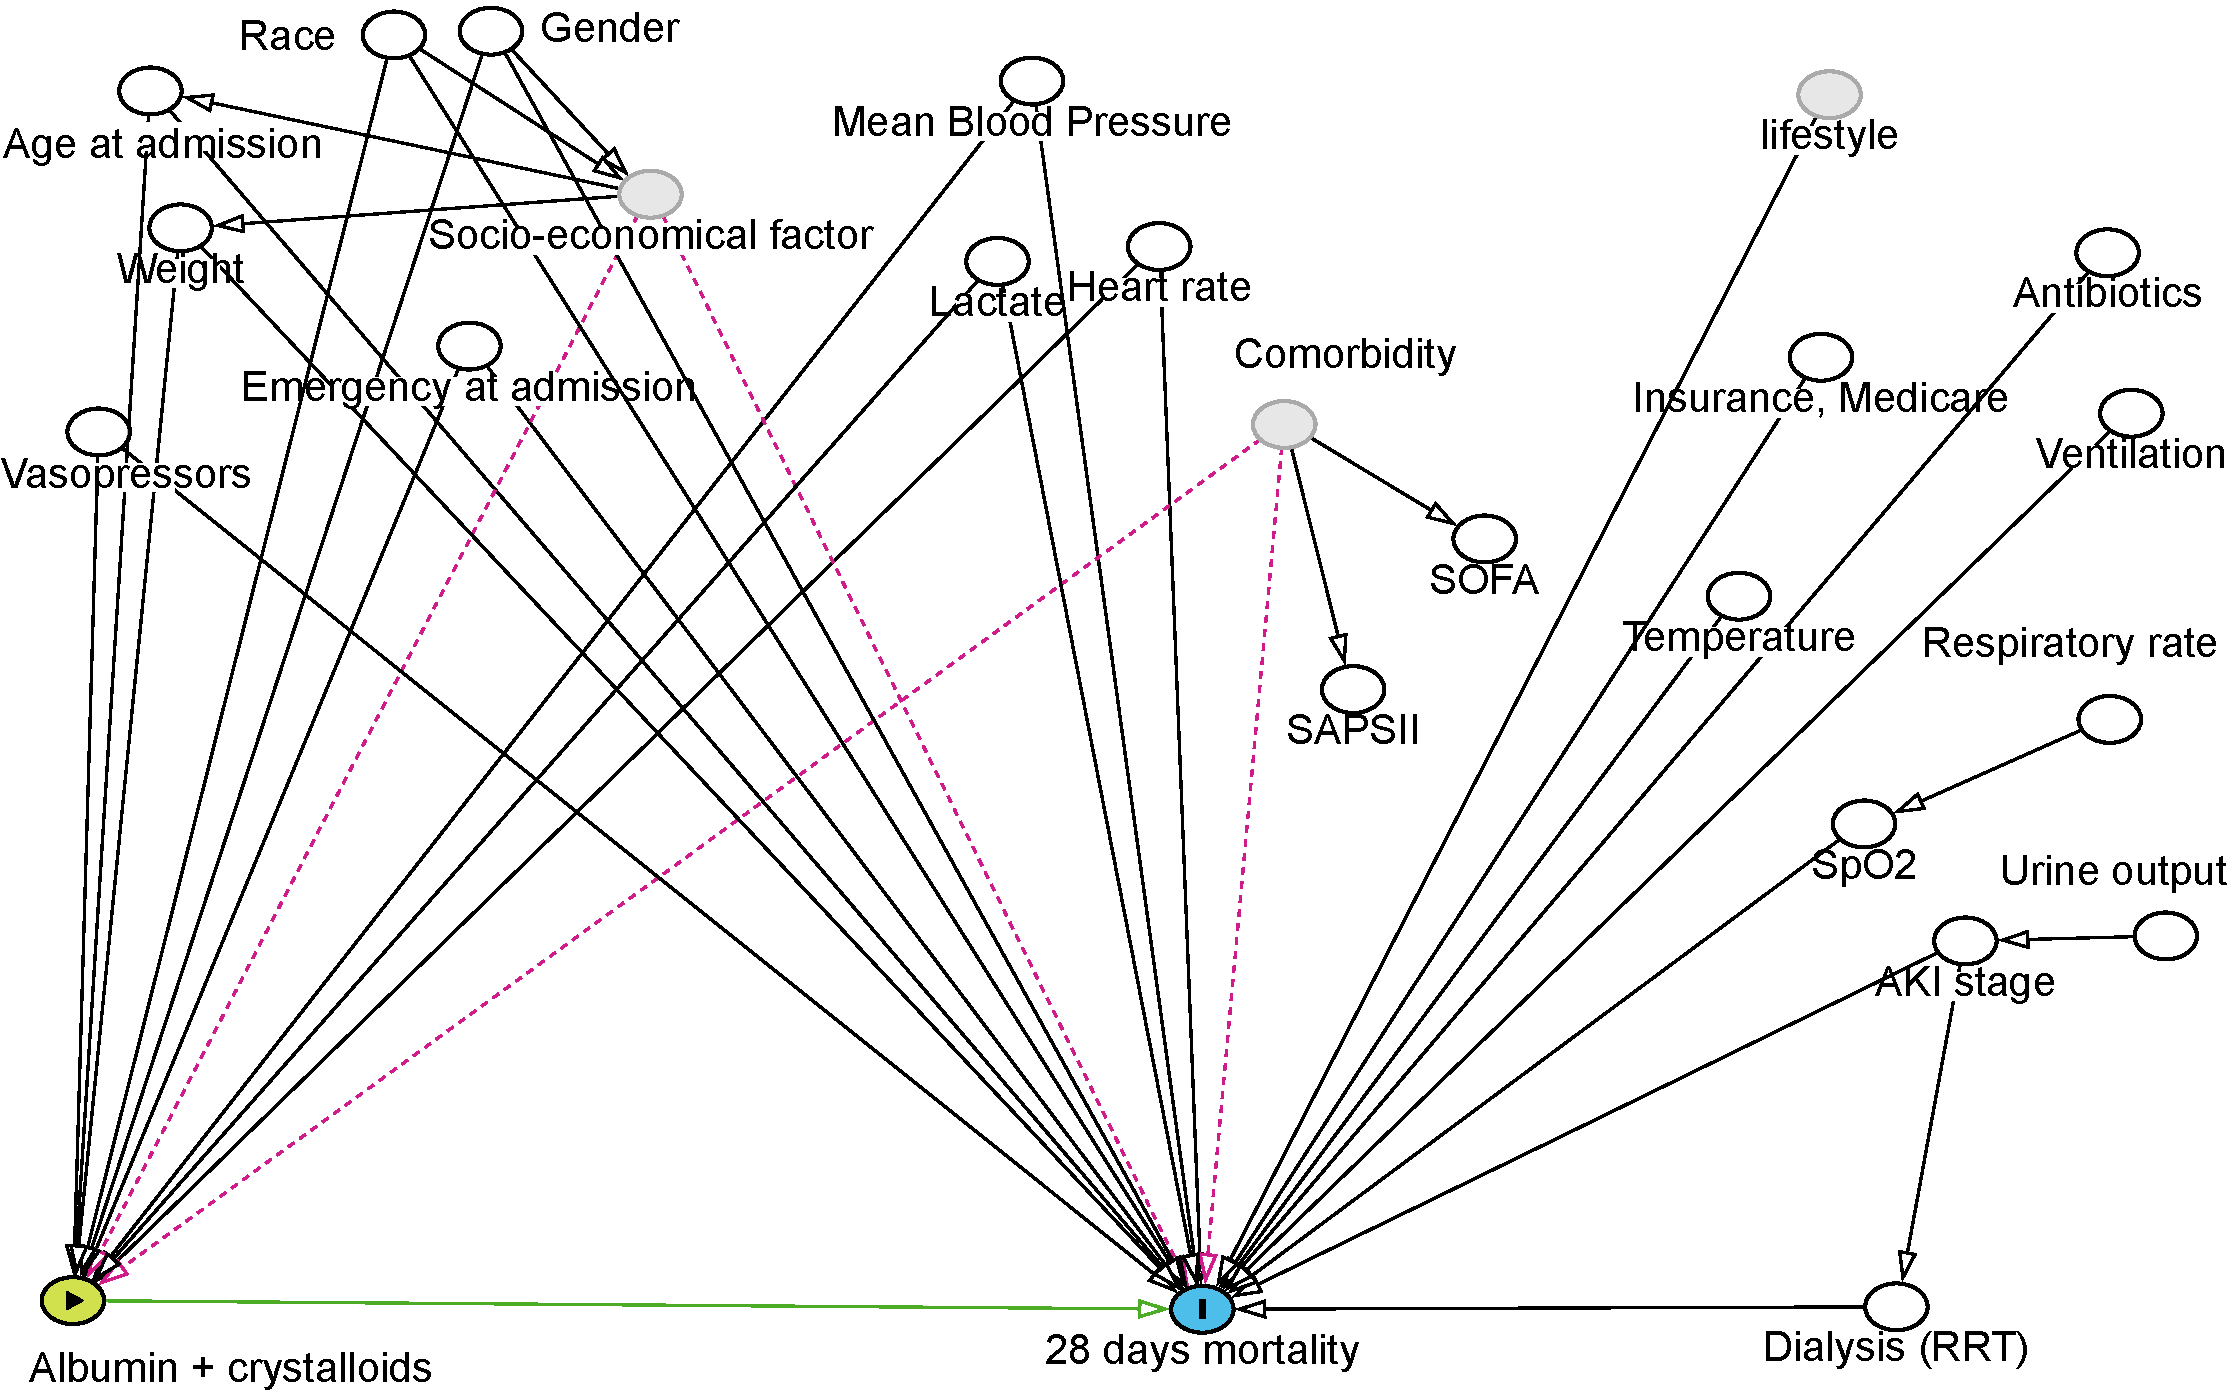
\includegraphics[width=.9\linewidth]{img/chapter_4/dagitty_graph.pdf}
  \caption{\textbf{Causal graph for the Albumin vs crystalloids emulated
      trial} -- The
    green arrow indicates the effect studied. Black arrows show causal links
    known to medical expertise. Dotted red arrows highlight confounders not directly
    observed. For readability, we draw only the most important edges from an
    expert point of view. All white nodes corresponds to variables included in
    our study.}\label{fig:causal_diagram_albumin}
\end{figure}


\subsection{Estimation}\label{subsec:causal_tuto:estimation_mimic}

\paragraph{Confounder aggregation:}

We tested multiple aggregations such as the last value before the start of the
follow-up period, the first observed value, and both the first and last values as
separated features.

\paragraph{Causal estimators:}

We implemented multiple estimation strategies, including Inverse Propensity
Weighting (IPW), outcome modeling (G-formula) with T-Learner, Augmented Inverse
Propensity Weighting (AIPW) and Double Machine Learning (DML). We used the
python packages dowhy \citep{sharma2018tutorial} for IPW implementation and
EconML \citep{battocchi2019econml} for all other estimation strategies.
Confidence intervals were estimated by bootstrap (50 repetitions).
Appendices \ref{apd:causal_estimators} and
\ref{apd:packages} detail the estimators and the available Python
implementations.

\paragraph{Outcome and treatment estimators:}

To model the outcome and treatment, we used two common but different estimators:
random forests and ridge logistic regression implemented with scikit-learn
\citep{pedregosa_scikitlearn_2011}. We chose the hyperparameters with a random search
procedure (detailed in Appendix \ref{apd:hyper_parameter_search}). While
logistic regression handles predictors in a linear fashion, random forests
should have the benefit of modeling non-linear relations as well.

\begin{figure}[h!]
  \centering
  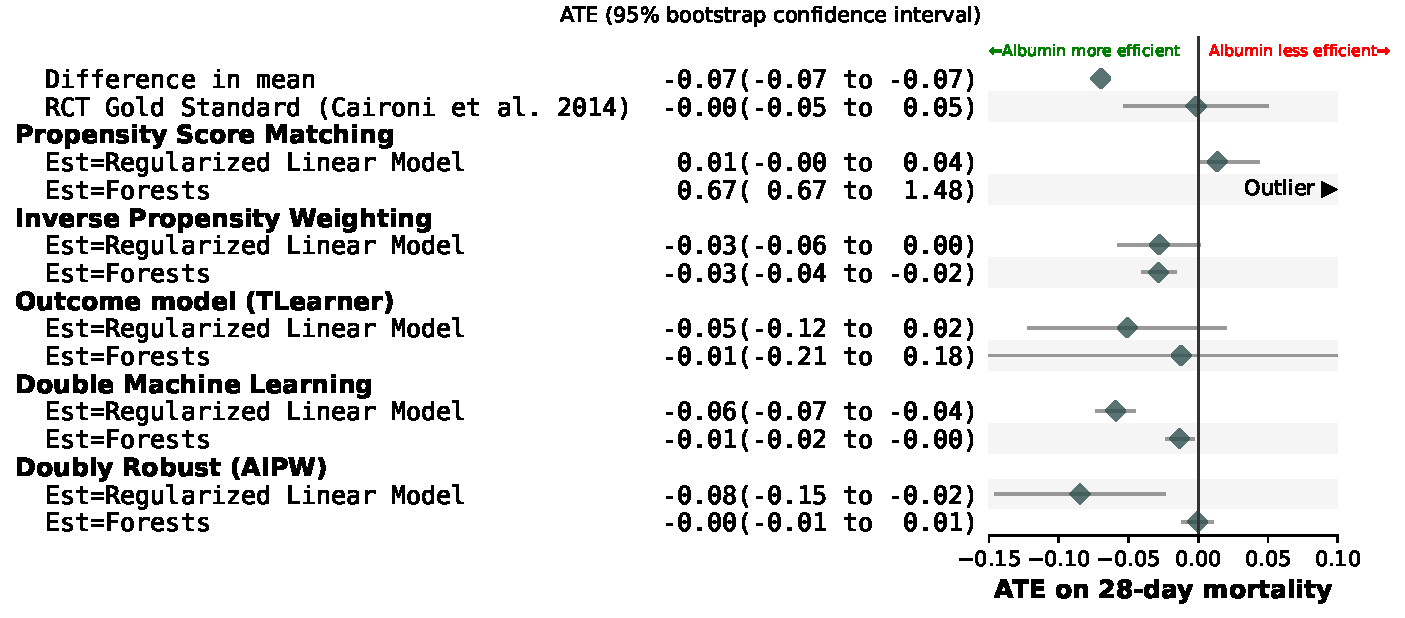
\includegraphics[width=\linewidth]{img/chapter_4/albumin_for_sepsis__obs_1d__estimates_20230712__est_lr_rf__bs_50.pdf}
  \caption{\textbf{Forest plot for the vibration analysis} -- Different
    estimators give different results, sometimes even outside of
    each-other's bootstrap confidence intervals. Score matching yields
    unconvincingly high estimates, inconsistent with the published RCT.
    With other causal approaches, using linear estimators for nuisances
    suggest a reduced mortality risk for albumin, while using forests for
    nuisance models points to no effect, which is consistent with the RCT gold standard.
    The diamonds
    depict the mean effect and the bar are the 95\% confidence intervals
    obtained by 50 bootstrap repetitions.}\label{fig:albumin_for_sepsis:results}
\end{figure}

\subsection{Vibration analysis: Understanding variance or sources of
  systematic errors in our study}\label{subsec:causal_tuto:vibration_mimic}

\paragraph{Varying estimation choices: Confounders aggregation, causal and nuisance estimators}

Figure \ref{fig:albumin_for_sepsis:results} shows varying confidence intervals
(CI) depending on the method. Doubly-robust methods provide the narrowest CIs,
whereas the outcome-regression methods have the largest CI. The estimates of the
forest models are closer to the consensus across prior studies (no effect) than the estimates
from the logistic regression indicating a better fit of the non-linear
relationships in the data.
We only report the first and last
pre-treatment feature aggregation strategies, since detailed analysis showed
little differences for other choices of feature aggregation (see Appendix
\ref{apd:detailed_results}).
%
Confronting this analysis with the prior published evidence of
little-to-no effect, it seems reasonable to select the models using
random forests for nuisance. Out of these, theory suggests to trust more
double machine learning or doubly robust approaches.


\paragraph{Study design -- Illustration of immortal time bias:}

To illustrate the risk of immortal-time bias, we varied the eligibility period
by allowing patients to receive the treatment or the control in a shorter or
longer time window than 24 hours. As explained in
Subsection \ref{subsec:causal_tuto:framing}, a large eligibility period
means that patients in the study are more likely to be treated if they survived
till the intervention and hence the study is biased to overestimate the
beneficial effect of the intervention. Figure
\ref{fig:albumin_for_sepsis:immortal_time_bias} shows that larger eligibility
periods change the direction of the estimate and lead to Albumin seeming
markedly more efficient. Should the analyst not have in mind the mechanism of
immortal time bias, this vibration analysis ought to raise an alarm and
hopefully lead to correct the study design.


\begin{figure}[h!]
  \centering
  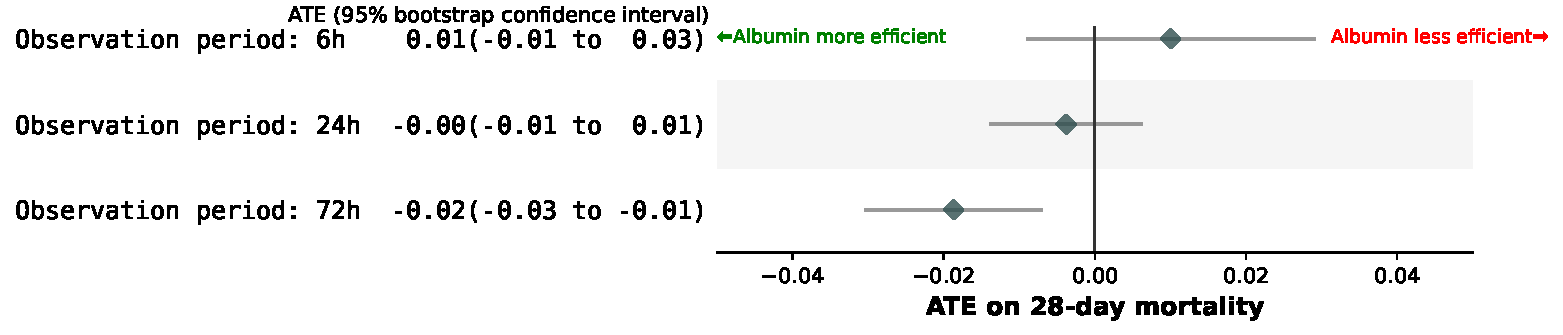
\includegraphics[width=\linewidth]{img/chapter_4/itb__immortal_time_bias_double_robust_forest_agg_first_last__bs_30.pdf}
  \caption{\textbf{Detecting immortal time bias} -- Increasing the observation period increases the temporal blank period
    between inclusion and treatment initialization, associating thus
    patients surviving longer with treatment: Immortal
    Time Bias. A longer observation period (72h) artificially favors the
    efficacy of Albumin. The estimator is a doubly robust learner (AIPW) with random
    forests for nuisances. This result is consistent across estimators as shown
    in Appendix \ref{apd:detailed_results_itb}. The green diamonds depict the
    mean effect and the bar are the 95\% confidence intervals obtained by 30
    bootstrap repetitions. }\label{fig:albumin_for_sepsis:immortal_time_bias}
\end{figure}


\subsection{Treatment heterogeneity: Which treatment for a given
  sub-population?}%
\label{subsec:causal_tuto:heterogeneity_mimic}%


We now study treatment heterogeneity using the pipeline validated by confronting
the vibration analysis to the literature: a study design avoiding immortal time
bias, and the double machine learning model using forest for nuisances and a
linear model for the final heterogeneity regression. We explore heterogeneity
along four binary patient characteristics, displayed on Figure
\ref{fig:albumin_for_sepsis:cate_results}. We find that albumin is beneficial
with patient with septic shock before fluid administration, consistent with the
\cite{caironi2014albumin} RCT. It is also beneficial for older patients (age
>=60) and males, consistent with \citep{zhou2021early}, as well as white patients.

\begin{figure}[!h]
  \begin{minipage}{.3\linewidth}
    \caption{The subgroup distributions of Individual Treatment effects showed
      better treatment efficacy for patients older than 60 years, septic shock,
      and to a lower extent males. The final estimator is ridge regression. The
      boxes contain the $25^\text{th}$ and $75^\text{th}$ percentiles of the CATE
      distributions with the median indicated by the vertical line. The whiskers
      extend to 1.5 times the inter-quartile range of the
      distribution.}\label{fig:albumin_for_sepsis:cate_results} \end{minipage}%
  \hfill%
  \begin{minipage}{.67\linewidth}
    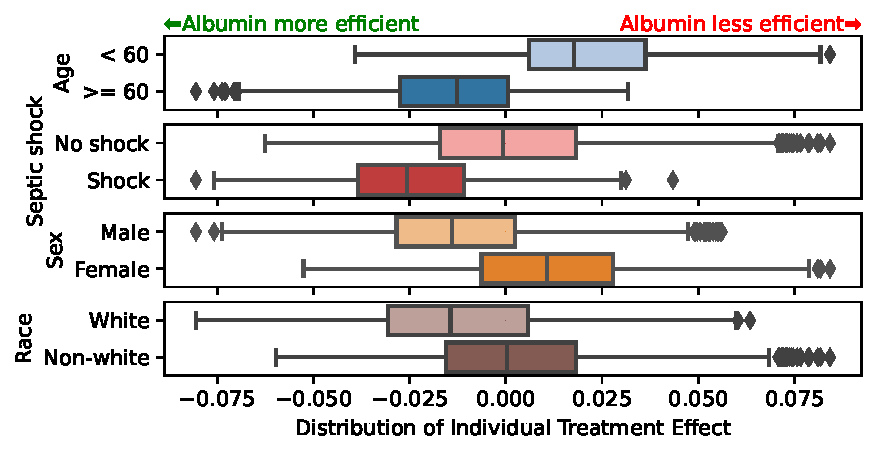
\includegraphics[width=\linewidth]{img/chapter_4/boxplot_est__DML__nuisances__Forests__final_Ridge.pdf}
  \end{minipage}%
\end{figure}

\section{Discussion and conclusion}\label{subsec:causal_tuto:discussion}


\paragraph{A didactic causal framework for decision-making from EHR} Our analytic framework strives to streamline extracting valid decision-making
rules from EHR data. Decision-making is tied to a choice: to treat or not
to treat, for a given intervention. A major pitfall, source of numerous
shortcuts of machine-learning systems, is to extract non-causal
associations between the intervention and the outcome. Our framework is
designed to avoid these pitfalls by starting with rigorous causal analysis, in the
form of a target trial, to validate study design and analytic choices
before more elaborate analysis, potentially using machine-learning for
individual predictions.
%
We argue that in the absence of a precise framing including treatment
allocation, automated decision making is brittle. It is all too easy, for
instance, to build a predictive system on post-treatment data, rendering
it unreliable for decision making.
%
EHR data come with particular challenges: information may be available
indirectly, \emph{e.g.} via billing codes, the time-wise dimension requires
aggregations (Sub-section \ref{subsec:causal_tuto:estimation}). These challenges can create
subtle causal biases (Subsection \ref{subsec:causal_tuto:framing}).
%
To ensure that our framework addresses all aspects of EHR analysis and to
expose it in a didactic way, we detailed a complete analysis of a publicly-available EHR dataset,
supported by \href{https://github.com/soda-inria/causal_ehr_mimic}{open code}.
% Now scare the reader: many moving parts, things can go wrong?

\paragraph{A well-framed target trial can be validated}

Assessing the validity of an analysis is challenging even for experts
\citep{ioannidis2005most,breznau2022observing}. Our framework recommends
using a well-specific target trial to establish a valid pipeline because
it helps confronting the resulting average treatment effect to other
evidence \citep{hernan_using_2016,wang2023emulation}. Our
resuscitation-fluid analysis matches well published findings:
Pooling evidence from high-quality RCTs, no effect of albumin in severe sepsis
was demonstrated for both 28-day mortality (odds ratio (OR) 0.93, 95\% CI
0.80-1.08) and 90-day mortality (OR 0.88, 95\% CI 0.76-1.01) \citep{xu2014comparison}. This consistency validates
our study design and analytic choices.
% The immortal time bias
Varying analytic choices and confronting them to prior studies can reveal
loopholes in the analysis, as we demonstrated with immortal time bias:
extending the time between ICU admission and intervention to 72 hours,
we observed an inflation of effect size consistent with such
bias. Looping back to reference RCTs reveals that these
include patients within 8
to 24 hours of ICU admission \citep{safe2011impact,annane2013effects,
  caironi2014albumin}.


\paragraph{Decision-making from EHRs}

Once the causal analysis has been validated, it can be used for decision
making. A sub-population analysis (as in
Figure \ref{fig:albumin_for_sepsis:cate_results}) can distill rules on
which groups of patients should receive the treatment. Ideally, dedicated
RCTs can be run with inclusion criteria matching these sub-groups.
However, the cost and the ethical concerns of running RCTs limit the
number of sub-groups that can be explored.
%
In addition, the sub-group view risks oversimplifying, as opposed to
patient-specific effect estimates to support more individualized clinical
decision making \citep{kent2018personalized}.  For this, predictive modeling
shines. Causally-grounded machine learning can give good counter-factual
prediction \citep{prosperi2020causal,hernan2019second,richens2020improving}, if
it predicts well the treated and untreated outcomes as shown in
\ref{sec:causal_model_selection:motivation}. Even without focusing on a specific
intervention, anchoring machine learning on causal mechanisms gives models that
are more robust to distributional shift \citep{scholkopf2021toward}, safer for
clinical use \citep{richens2020improving}, and more fair
\citep{plecko2022causal}.
%
Capturing individualized effects via machine-learning models does require
to probe many diverse individuals. EHRs and claims data are well suited
for these models, as they easily cover much more individuals
than a typical clinical study.

% Loop to limitations by saying that learning on EHR cannot inform on
% trade-offs that have never been explored in the data

\paragraph{EHRs and RCTs, complementary sources of evidence} But EHRs cannot inform on trade-offs that have not been explored in the
data. No matter how sophisticated, causal inference cannot conclude if
there is no data to support an apple-to-apple comparison between treated
and non-treated individuals. For example, treatment allocation is known
to be influenced by race- and gender-concordance between the patient and the
care provider. Yet, if the EHR data does no contain this information, it
cannot nourish evidence-based decisions on such matter.
%
EHRs and RCTs complement each other:
a dedicated study, with a randomized intervention, as an RCT, can be
crafted to answer a given question on a given population. But RCTs cannot
address all the subpopulations, local practices, healthcare systems
\citep{rothwell2006factors,travers2007external,kennedy2015literature}.
Our framework suggest to integrate the evidence from RCTs designed with
matching PICO formulation to ensure the validity of the analysis and to
use the EHR to explore heterogeneity.


\paragraph{Conclusion}

Without causal thinking machine learning does not suffice for optimal
clinical decision making for each and every patient. It will replicate
non-causal associations such as shortcuts improper for decision making.
As models can pick up information such as race implicitly from the data
\citep{adam2022write}, they risk propagating biases when building AI
models which can further reinforce health disparities. This problem is
acknowledged by the major tech companies which are deploying
causal inference tooling to mitigate biases
\citep{tensorflow_responsible_ai, microsoft_responsible_ai, pwc_responsible_ai}.
%
On the medical side, causal modeling can create actionable
decision-making systems that reduce inequities
\citep{mitra2022future,ehrmann2023making}.
%
However, as we have seen, subtle errors can make an intervention seemingly more
--or less-- beneficial to patients. No sophisticated data-processing
tool can safeguard against invalid study design or modeling choices.
%
The goal of our step-by-step analytic framework is to help the data
analyst work around these loopholes, building models that avoid shortcuts
and extract the best decision-making evidence.
%
Applied to study the addition of albumin to crystalloids to
resuscitate sepsis patients, it shows that this addition is not
beneficial in general, but that it does improve survival on
specific individuals, such as patients undergoing sceptic shock.

%% Not necessary and a bit artificial: Better to let the transistion between chapters into abstracts.
% To select estimators, we used statistical insights and vibration analysis
% without looking at their predictive performances. On the contrary, machine
% learning rely solely on out-of-bag performances for these choices. In the next
% chapter, we will investigate why this technique does not work when selecting predictive
% models for causality, and which corrections can be applied.


%%%%%%%%%%%%%%%%%%%%%%% CHAPTER 5 %%%%%%%%%%%%%%%%%%%%%%%%%%%%%%%
\chapter{How to select predictive models for causal inference?}%
\label{chapter:causal_model_selection}%

\begin{citationbox}
  Nature marks each growth ... according to its curative benefit.
  \par\hfill -- Paracelsus
\end{citationbox}

\begin{chapterabstract}
  % Predictive models are not sufficient for decision making: I showed it in
  % chapter 4
  In the previous chapters, we showed the strong interest in predictive models for
  healthcare, bridging to increasingly complex machine learning algorithms. We
  also pointed out that even when giving likely outcomes, they are not immediately
  transposable to decision making --choosing whether to treat or not to treat.
  Such reasoning on the effect of an intervention is a causal-inference task. We
  demonstrated that causal thinking was necessary to avoid introducing biases in
  the study design or during confounders selection.
  % Even with causal framework, there are too many models to choose from
  But, even with a robust causal framework such as in Chapter 4, the
  practitioner is left to choose among the plethora of predictive models
  available for health data (some detailed in
  \ref{subsec:predictive_models:importance}). In a given situation, which of
  these models yield the most valid causal estimates?
  % scope of the paper 
  Here, we highlight that classic machine-learning model selection does not pick
  the best models for causal inference. Indeed, causal model selection should
  control both outcomes for each individual, treated or not treated, whereas only
  one outcome is observed.
  Theoretically, simple risks used in machine learning do not control causal
  effects when treated and non-treated population differ too much. More elaborate
  risks use ``nuisances'' re-weighting to approximate the causal error on the
  observed data. But does estimating these nuisances adds noise to model selection?
  % Contributions
  Drawing from an extensive empirical study, we outline an efficient causal
  model-selection procedure. To select the best predictive model to guide
  decisions: use the so-called $R\text{-risk}$, use flexible estimators to compute
  the nuisance models on the train set, and split out 10\% of the data to compute
  risks.
\end{chapterabstract}
%\section*{Abstract}\label{sec:causal_model_selection:abstract}

\vfill

\begin{flushright}
  \begin{minipage}{15cm}
    {\small{This chapter corresponds to the article entitled \textit{How to select
          predictive models for decision making or causal inference?}
        \underline{submitted} to \textit{Artificial
          Intelligence in Medicine},}}\\

    {\small\hfill{}Authors: Matthieu Doutreligne, Gaël \textsc{Varoquaux}.}
  \end{minipage}
\end{flushright}

\clearpage
\minitoc

\section{Motivation: causal predictive models cannot rely on the Machine Learning
  toolbox}\label{sec:causal_model_selection:motivation}

\subsection{Extending prediction to prescription needs causality}\label{subsec:causal_model_selection:extending_prediction}

\paragraph{Progress in machine learning brings predictive models to new health
  data} \citep{beam2018big,rajkomar2019machine}, with the promise of precision
medicine. Automated analysis of medical images is increasingly accurate,
\emph{eg} for brain images, \citep{khojaste2022deep,zhang2019radiological} or
mammography \citep{yala2019deep,shen2019deep,nassif2022breast}. New prognostic
models leverage routinely-collected patient records \citep{mooney2018bigdata}:
predicting heart failure from claims \citep{desai2020comparison}, suicide
attempts from questionnaires \citep{simon2018predicting}... Clinical notes
contain much prognostic information but require text modeling
\citep{horng2017creating,wang2020prediction,spasic2020clinical,
  jiang2023health}. Data may be difficult to control and model, but the accuracy
of the prediction can be verified on left-out data
\citep{altman2009prognosis,poldrack2020establishment,varoquaux2022evaluating}.
Given a model predicting a health outcome, precision medicine would like it to
guide decisions: will an individual benefit from an intervention such as
surgery \citep{fontana2019can}? Contrasting predictions with and without the
treatment gives an answer, but statistical validity requires causal inference
\citep{snowden_implementation_2011,blakely2020reflection}.

% - Causal inference is difficult
% - Beyond the dream of assessing effectiveness and safety in real-word
%   practice \citep{black1996we} include off-label drug usage 
%   \citep{radley2006off} (which may lead to drug repurposing)
% - Plug in that outcome modeling is complementary to RCTs: observational
%   data gives weaker evidence than trials, but on both data outcome
%   modeling opens the door to individual.
% - Epidemiology has focused on propensity-score methods
% - Principle causal inference with outcome models is possible
% - It brings the promises of \emph{individualized treatment effects} --a
%   goal related to capturing heterogeneity and thus CATE--
% - It also performs well on causal-inference competition, although they
%   focused on the ATE

% The plethora of approaches approaches give different causal-inference
% estimates => need for guideline on causal model selection.

\paragraph{Causal-inference bridges to predictive modeling via the rich statistical literature on \emph{outcome
    models},} or G-computation, G-formula \citep{robins_role_1986}, Q-model \citep{snowden_implementation_2011}, conditional
mean regression \citep{wendling_comparing_2018}. A central challenge of inference of treatment effects is that of
confounding: spurious associations between treatment allocation and baseline health, \emph{eg} only prescribing a drug
to mild cases \citep{hernan_causal_2020,vanderweele2019principles}. Controlled allocation of treatment, as in randomized
controlled trials (RCTs), alleviate this concern. Yet most machine-learning models are trained on \emph{observational}
data, close to real-word practice \citep{black1996we,hernan_methods_2021} but challenging for causal inference. Causal
inference has been central to epidemiology, typically with methods that model treatment assignment
\citep{austin2015moving,grose_use_2020}, based on propensity scores \citep{rosenbaum_central_1983}. Recent empirical
results \citep{wendling_comparing_2018,dorie_automated_2019} show benefits of outcome modeling to estimate average
treatment effects. Maybe a greater benefit is that these methods naturally go beyond average effects, estimating
individualized or conditional average treatment effects (CATE), central to precision medicine.
%
For this purpose, such methods are also invaluable on randomized trials
\citep{su2018random,lamont2018identification,hoogland2021tutorial}.

\paragraph{Explosion of outcome modeling or machine learning methods.}
Many deep-learning methods have been developed for medical
image analysis \citep{shen2017deep,monshi2020deep}.
Even outcome-modeling methods specifically designed for causal
inference are numerous: Bayesian Additive Regression Trees
\citep{hill_bayesian_2011}, Targeted Maximum Likelihood Estimation
\citep{laan_targeted_2011,schuler_targeted_2017}, causal boosting
\citep{powers_methods_2018}, causal multivariate adaptive regression
splines \citep{powers_methods_2018}, random forests
\citep{wager_estimation_2018, athey_generalized_2019},
Meta-learners \citep{kunzel_metalearners_2019}, R-learners
\citep{nie_quasioracle_2017}, Doubly robust estimation
\citep{chernozhukov_double_2018}...
%\idea{The variety of estimators calls for model selection procedures}
The wide variety of methods raises the problem
of selecting between different estimators based on the data at hand.
%
Indeed, estimates of treatment effects can vary markedly across different
predictive models. For instance, Figure \ref{fig:acic_2016_ate_heterogeneity} shows
large variations obtained across different outcome estimators on
semi-synthetic datasets \citep{dorie_automated_2019}. Flexible models
such as random forests are doing well in most settings except
when treated and untreated populations differ noticeably, in
which case a linear model (ridge) is to be preferred.
However random forests with different hyper-parameters
(max depth= 2) yield poor estimates.
A simple rule of thumb such as preferring flexible models does not work in
general; model selection is needed.

\begin{figure}[h!]
  \begin{minipage}{.3\linewidth}
    \caption{\textbf{Different outcome models lead to different
        estimation errors on the Average Treatment Effects},
      on 77 classic simulations with known true causal effect
      \citep{dorie_automated_2019}. The different models are ridge regression
      and random forests with different hyper-parameters
      (details
      \ref{apd:toy_example:acic_2016_ate_variability}). The different configurations are
      plotted as a function of increasing difference between treated and
      untreated population --see
      \autoref{subsec:causal_model_selection:measuring_overlap}.
      There is no systematic best performer; data-driven model
      selection is important.
      \label{fig:acic_2016_ate_heterogeneity}
    }
  \end{minipage}
  \hfill
  \begin{minipage}{.65\linewidth}
    %\centering
    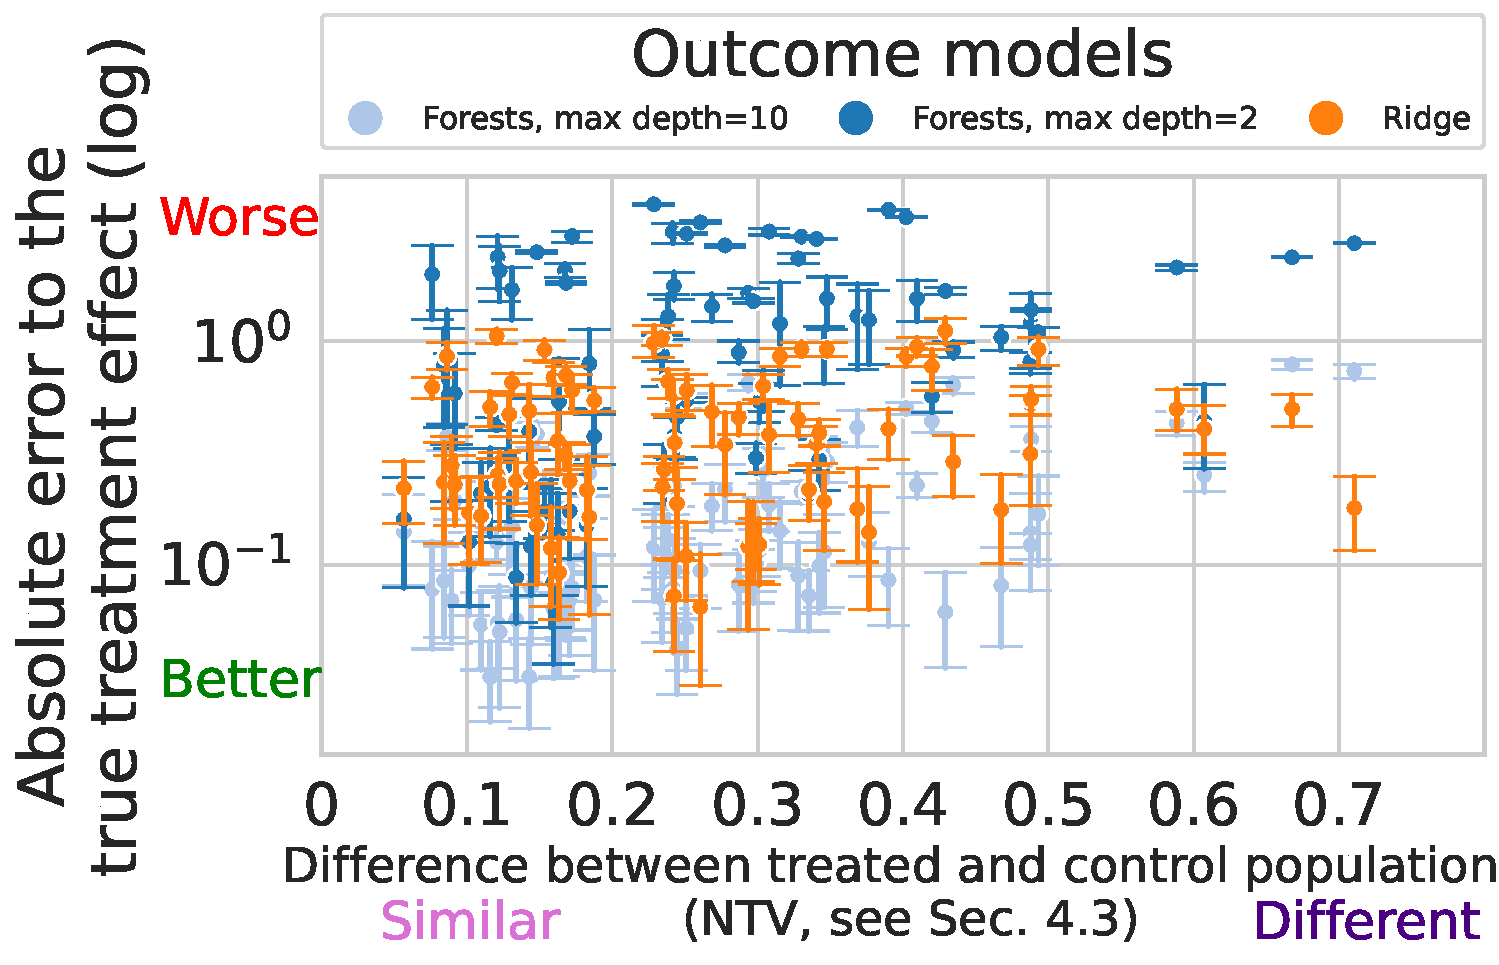
\includegraphics[width=\linewidth]{img/chapter_5/_2023-03-08-11-10-28_acic_2016_ate_heterogeneity.parquet_abs_bias_ylog_scale=True.pdf}%
  \end{minipage}
\end{figure}

Standard practices to select models in predictive settings rely on
the error on the outcome
\citep{poldrack2020establishment,varoquaux2022evaluating}. However, as we
will see, these practices may not pick the best models
for causal inference, as they can be misled by inhomogeneities due to
treatment allocation.
%
Given complex, potentially noisy, data, which model is to be most trusted to
yield valid causal estimates? As no single learner performs
best on all data sets, there is a pressing need for clear guidelines to select
outcome models for causal inference.

\paragraph{Objectives and structure of the chapter}

In this chapter, we study \textit{model selection procedures}
in practical settings: \textit{finite samples} settings and without
\textit{well-specification} assumption. Asymptotic causal-inference
theory calls for complex risks, but a practical question is
whether model-selection procedures, that rely on data split, can estimate
these risks reliably enough. Indeed, they
come with more quantities to estimate, which may
bring additional variance, leading to worse model selection.

We first illustrate the problem of causal model
selection and briefly review prior art. Then, Section
\ref{sec:causal_model_selection:setting} sets causal model selection in the
\emph{potential outcome} framework and details the causal risks and
model-selection procedure. Section \ref{sec:theory} gives theoretical
results. Section \ref{sec:empirical_study} details a thorough empirical
study, covering many different settings. Finally, Section \ref{sec:discussion}
discusses the findings.
%
Results outline how to best select outcome models for causal
inference with an adapted
cross-validation to estimate the so-called $R\mathrm{-risk}$.
This risk compensates for systematic
differences between treated and non-treated individuals using
two \emph{nuisance} models,
themselves estimated from data and thus imperfect; yet these
imperfections do not undermine the $R\mathrm{-risk}$.


\subsection{Illustration: the best predictor may not estimate best causal
  effects}%
\label{subsec:causal_model_selection:illustration}%


\begin{figure}[t!]
  \begin{minipage}{0.32\textwidth}
    \caption[The best predictor may not estimate best causal
      effects]{\textbf{Illustration} \\a) a random-forest estimator
      with high performance for standard prediction (high $R^2$) but that
      yields poor causal estimates (large error between true effect $\tau$ and
      estimated $\hat{\tau}$), b) a linear estimator with smaller
      prediction performance leading to better causal estimation. \\[1ex]
      Selecting the estimator with the smallest error to the individual
      treatment effect $\mathbb{E}[(\tau(x) - \hat{\tau}(x))^2]$
      --the $\tau\text{-risk}$, def.\,\ref{def:tau_risk} -- would lead to
      the best causal estimates; however computing this error is not
      feasible: it requires access to unknown quantities:
      $\tau(x)$. \\[1ex]
      While the random forest fits the data better than the linear model, it
      gives worse causal inference because its error is inhomogeneous between
      treated and untreated. The $R^2$ score does not capture this
      inhomogeneity.
      \label{fig:toy_example}
    }
  \end{minipage}
  \hfill
  \begin{minipage}{0.65\textwidth}
    %\centering
    {\sffamily\footnotesize\scalebox{0.9}{a) Random forest, good average prediction but bad
        causal inference}}

    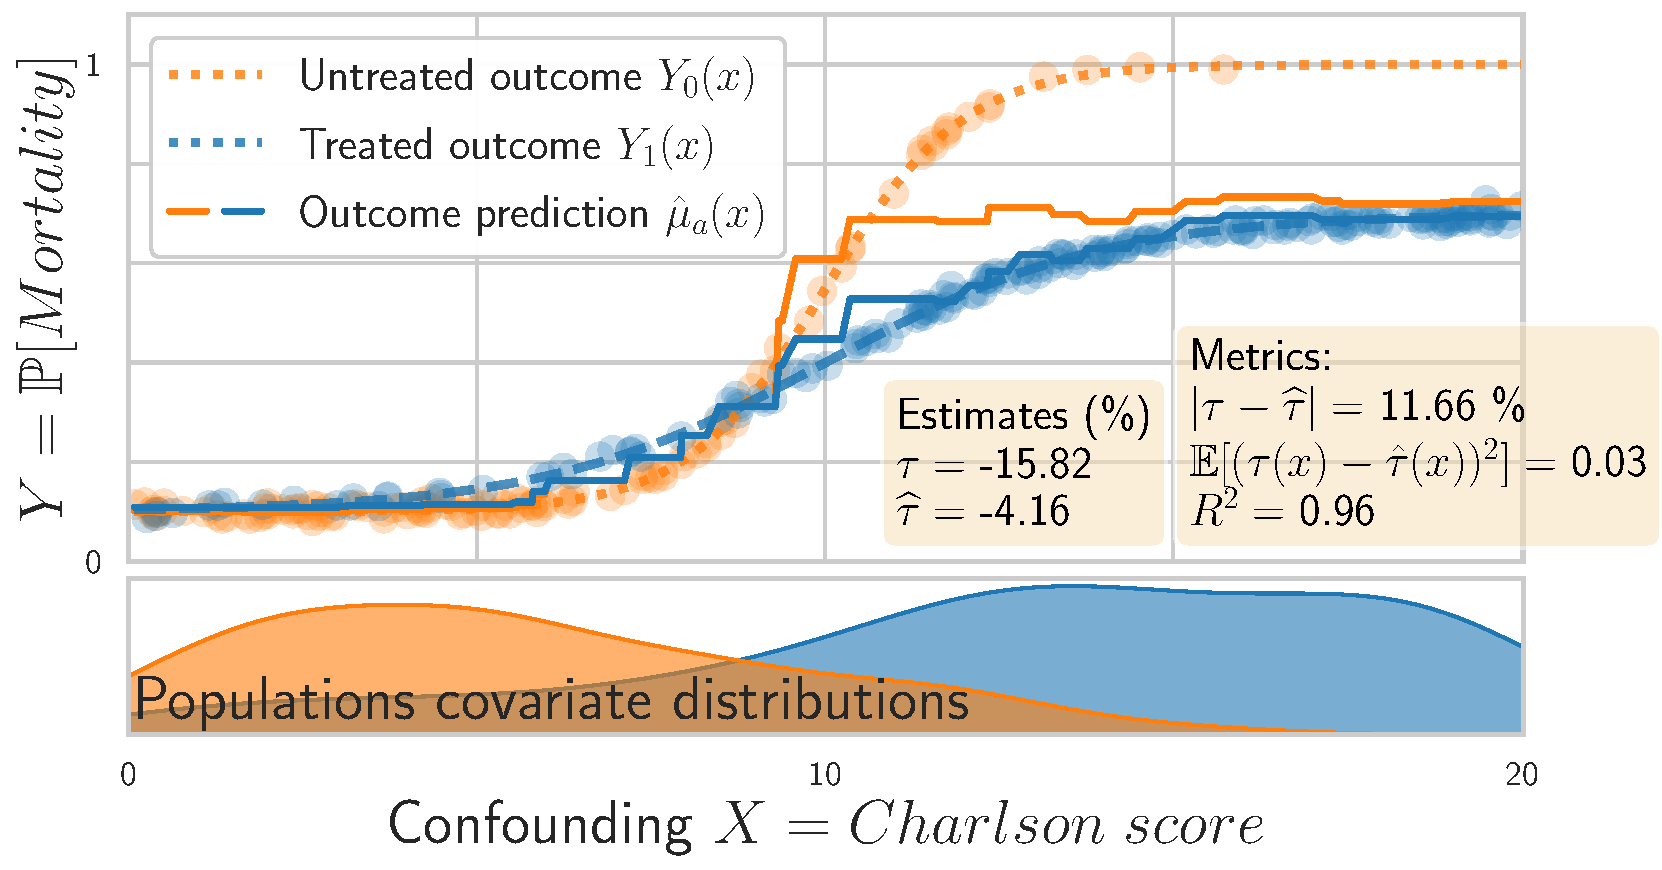
\includegraphics[width=1\linewidth]{img/chapter_5/toy_random_forest_high_R2_high_tau_risk.pdf}%

    {\sffamily\footnotesize\scalebox{0.9}{b) Linear model, worse average
        prediction but better causal inference}}

    \hfill%
    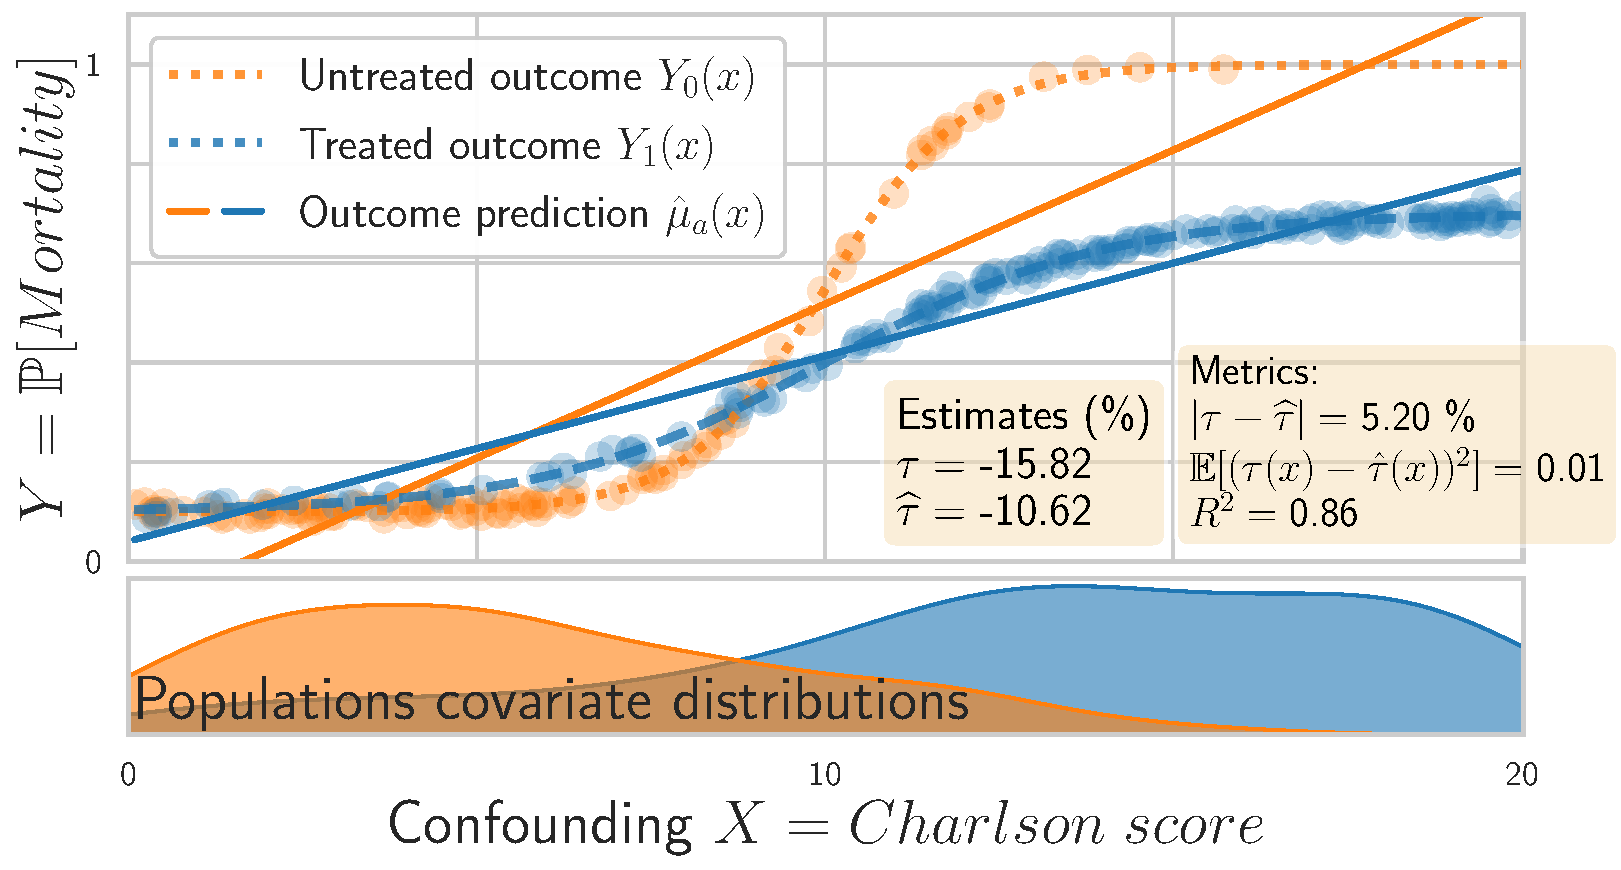
\includegraphics[width=1\linewidth]{img/chapter_5/toy_tlinear_model_small_R2_small_tau_risk.pdf}%
  \end{minipage}
\end{figure}


Using a predictor to reason on causal effects relies on contrasting the
prediction of the outcome for a given individual with and without the
treatment --as detailed in \autoref{sec:causal_model_selection:setting}.
%
Given various predictors of the outcome, which one should we use?
%
Standard predictive modeling or machine-learning practice selects the
predictor that minimizes the expected error.
However, this predictor may not be the best model to reason about
causal effects of an intervention, as we illustrate below.

Figure \ref{fig:toy_example} gives a toy example: the probability $Y$ of
an undesirable
outcome (\emph{eg} death), a binary treatment $A \in \{0, 1\}$, and a covariate
$X \in \mathbb R$ summarizing the patient health status (eg. the
Charlson index \citep{charlson_new_1987}). We simulate a
treatment beneficial (decreases $Y$) for patients with high Charlson scores (bad health
status) but with little effect for patients in good
condition (low Charlson scores).


Figure \ref{fig:toy_example}a shows a random forest predictor with a
counter-intuitive behavior: it predicts well on average the outcome (as measured
by a regression $R^2$ score) but perform poorly to estimate causal quantities:
the average treatment effect $\tau$ (as visible via the error $|\tau -
  \hat{\tau}|$) or the conditional average treatment effect (the error
$\mathbb{E}[(\tau(x) - \hat{\tau}(x))^2]$, called CATE).
%
On the contrary, Figure \ref{fig:toy_example}b shows a linear model with
smaller $R^2$ score but better causal inference.%

The problem is that causal estimation requires controlling
an error on both treated and non-treated outcome for the same individual:
the observed outcome, and the non-observed \emph{counterfactual} one.
The linear model is misspecified --the outcome functions are not
linear--, leading to poor $R^2$; but it interpolates better to regions
where there are few untreated individuals --high Charlson score-- and
thus gives better causal estimates. Conversely, the random forest puts
weaker assumptions on the data, thus has higher $R^2$ score but is biased
by the treated population in the poor-overlap region, leading
to bad causal estimates.

This toy example illustrates that the classic minimum Mean Square Error
criterion is not suited to choosing a model among candidate
estimators for causal inference.

\subsection{Prior work: model selection for outcome modeling (g-computation)}\label{subsec:causal_model_selection:prior_work}%


A natural way to select a predictive model for causal inference would be
an error measure between a causal quantity such as the CATE and models' estimate. But such error is
not a ``feasible'' risk: it cannot be computed solely from observed data
and requires oracle knowledge.

% XXX: I think that I should make the following paragraph shorter

\paragraph{Simulation studies of causal model selection}

Using eight simulations setups from \cite{powers_methods_2018}, where
the oracle CATE is known, \citet{schuler_comparison_2018} compare four
causal risks, concluding that for CATE estimation the best
model-selection risk is the so-called $R\text{-risk}$
\citep{nie_quasioracle_2017} --def.\,\ref{def:r_risk}, below. Their
empirical results are clear for randomized treatment allocation but less
convincing for observational settings where both simple Mean Squared
Error --MSE, $\mu\text{-risk}(f)$ def.\,\ref{def:mu_risk}-- and
reweighted MSE --$\mu\text{-risk}_{IPW}$ def.\,\ref{def:mu_ipw_risk}--
appear to perform better than $R\text{-risk}$ on half of the simulations.
Another work \citep{alaa_validating_2019} studied empirically both MSE and
reweighted MSE risks on the semi-synthetic ACIC 2016 datasets
\citep{dorie_automated_2019}, but did not include the $R\text{-risk}$. We complete these
prior empirical work by studying a wider variety of data generative
processes and varying the influence of overlap, an important parameter of
the data generation process which makes a given causal metric appropriate
\citep{damour_overlap_2020}. We also study how to best adapt
cross-validation procedures to causal metrics which themselves come with
models to estimate.

\paragraph{Theoretical studies of causal model selection}

Several theoretical works have proposed causal model selection procedures
that are \emph{consistent}: select the best model in a family given
asymptotically large data. These work rely on introducing a
CATE estimator in the testing procedure: matching
\citep{rolling_model_2014}, an IPW estimate
\citep{gutierrez_causal_2016}, a doubly robust estimator
\citep{saito_counterfactual_2020}, or debiasing the error with influence
functions \citep{alaa_validating_2019}. However, for theoretical
guarantees to hold, the test-set correction needs to converge to the
oracle: it needs to be flexible enough --well-posed-- and asymptotic
data. From a practical perspective, meeting such requirements
implies having a good CATE estimate, thus having solved
the original problem of causal model selection.

\paragraph{Statistical guarantees on causal estimation procedures}

Much work in causal inference has focused on procedures that
guarantee asymptotically consistent estimators, such as Targeted
Machine Learning
Estimation (TMLE) \citep{laan_targeted_2011,schuler_targeted_2017} or
Double Machine Learning \citep{chernozhukov_double_2018}. Here also, theories require asymptotic regimes and
models to be \textit{well-specified}.

By contrast, \citet{johansson2022generalization} studies causal estimation
without assuming that estimators are well specified. They derive an upper bound
on the oracle error to the CATE ($\tau\text{-risk}$) that involves the error on
the outcome and the similarity of the distributions of treated and control
patients. However, they use this upper bound for model optimization,
and do not give insights on model selection. In addition, for hyperparameter
selection, they rely on a plugin estimate of the $\tau\text{-risk}$ built with
counterfactual nearest neighbors, which has been shown ineffective
\citep{schuler_comparison_2018}.


\begin{background_box_left}

  \section{Formal setting: causal inference and model selection}%
  \label{sec:causal_model_selection:setting}%

  \subsection{The Neyman-Rubin Potential Outcomes framework}%
  \label{subsec:causal_model_selection:framework}%

  \paragraph{Settings} We consider the Potential Outcomes framework introduced in
  \ref{par:intro:causal_framework:neyman_rubin}.

  \paragraph{Causal assumptions}\label{par:causal_assumptions}

  Assumptions are necessary for causal estimands to be
  identifiability
  in observational settings \citep{rubin_causal_2005}. We assume the usual
  strong ignorability assumptions: \emph{1)}
  \emph{unconfoundedness} \mbox{$\{Y(0),
      Y(1) \} \indep A | X$}, \emph{~2)} \emph{strong overlap} ie. every patient has a
  strictly positive probability to receive each treatment, \emph{3)}
  \emph{consistency}, and \emph{4)} \emph{generalization} (introduced in
  \ref{subsec:causal_tuto:identification}).

  \paragraph{Estimating treatment effects with outcome models}\label{subsec:estimators}

  Should we know the two expected outcomes for a given $X$,
  we could compute the
  difference between them, which gives the causal effect of the treatment.
  %
  These two expected outcomes can be computed from the observed data:
  the consistency \ref{assumption:consistency} and unconfoundedness
  \ref{assumption:ignorability} assumptions imply the equality of two different
  expectations:
  \begin{equation}\label{eq:mu_identification}
    \mathbb E_{Y(a) \sim \mathcal{D^{\star}}} [Y(a)|X=x] = \mathbb E_{Y \sim \mathcal{D}} [Y|X=x, A=a]
  \end{equation}
  On the left, the expectation is taken on the counterfactual unobserved
  distribution. On the right, the expectation is taken on the factual observed
  distribution conditionally on the treatment. This equality is referred as the
  g-formula identification \citep{robins_new_1986}. For the rest of the
  paper, the expectations will always be taken on the factual observed
  distribution $\mathcal{D}$. This identification leads to outcome based estimators (ie.
  g-computation estimators \citep{snowden_implementation_2011}), targeting the
  ATE $\tau$ with outcome modeling:
  \begin{eqnarray}
    \tau =& \mathbb E_{Y \sim \mathcal{D^{\star}}}[Y(1) - Y(0)|X=x]
    = \mathbb E_{Y \sim \mathcal{D}}[Y|A=1] - \mathbb E_{Y \sim \mathcal{D}}[Y| A=0]
    \label{eq:tau_population}
  \end{eqnarray}
  This equation builds on two quantities: the conditional expectancy
  of the outcome given the covariates and either
  treatment or no no treatment, called \emph{response function}:
  \begin{flalign*}
    \text{Response function}
     &  &
    \mu_{a}(x) \myeq \; \mathbb E_{Y \sim \mathcal{D}} [Y|X=x, A=a]
     &  &
  \end{flalign*}

  Given a sample of data and the oracle response functions $\mu_0, \mu_1$, the
  finite sum version of \autoref{eq:tau_population} leads to an
  estimator of the ATE written:
  \begin{equation}
    \hat \tau = \frac{1}{n} \biggl(\sum_{i=1}^n \mu_{1}(x_i) - \mu_{0}(x_i) \biggr)
    \label{eq:ate_estimate}
  \end{equation}
  This estimator is an oracle \textbf{finite sum estimator} by opposition to the
  population expression of $\tau$, $\mathbb{E}[\mu_{1}(x_i) - \mu_{0}(x_i)]
  $,
  which involves an expectation taken on the full
  distribution $\mathcal D$, which is observable but requires infinite data. For
  each estimator $\ell$ taking an expectation over $\mathcal D$, we use the symbol
  $\hat \ell$ to note its finite sum version.

  Similarly to the ATE, at the individual level, the CATE:
  \begin{equation}
    \tau(x) = \mu_{1}(x) - \mu_{0}(x)
    \label{eq:cate_estimate}
  \end{equation}

  \paragraph{Robinson decomposition}
  The \emph{R-decomposition}
  of the outcome model plays an important role,
  \citep{robinson_rootnconsistent_1988}:
  introducing two quantities, the conditional mean outcome
  and the probability to be treated (known as propensity score \citep{rosenbaum_central_1983}):
  \begin{flalign}
    \text{Conditional mean outcome} &                    & m(x) \myeq \; & \mathbb E_{Y \sim
    \mathcal{D}} [Y|X=x]            &                    &
    \label{def:m}
    \\
    \text{Propensity score}         &                    &
    e(x) \myeq \;                   & \mathbb P[A=1|X=x]
    \label{def:propensity_score}
  \end{flalign}
  the outcome can be written
  \begin{flalign}\label{eq:r_decomposition}
    \text{R-decomposition}                                                                   &  & y(a) = m(x) + \big( a - e(x) \big)
    \tau(x) + \varepsilon(x; a) \quad \text{with}\quad \mathbb E[\varepsilon(X; A)|X, A] = 0 &  &
  \end{flalign}
  $m$ and $e$ are often called
  \emph{nuisances} \citep{chernozhukov_double_2018}; they are unknown.

\end{background_box_left}

%As noted by \citep{johansson2022generalization}, the machine learning
%community often referred to the CATE by ITE, the Individual Treatment Effect.
%From a purely causal point of view, the ITE is uniquely defined for each
%individual and might not be accessible: $ITE(x_i) = Y_i(1) -  Y_i(0)$. On the
%contrary, the CATE can always be derived by taking conditional expectancies. It
%is the expected effect of the treatment in the region of the covariate space
%around X. %Too cultivate

\begin{table*}[!tb]
  %\makebox[\textwidth]{
  \caption{Review of causal risks
    ---
    The $R\text{-risk}^*$ is called $\tau \text{-risk}_R$ in
    \citet{schuler_comparison_2018}.
    \label{tab:evaluation_metrics}}
  \resizebox*{\textwidth}{!}{
    \begin{threeparttable}[b]
      \centering
      \begin{tabular}{llr}
        \toprule
        Risk                                                                                           & Equation
                                                                                                       & Reference                                                                                                                                           \\
        \midrule
        $mse(\tau(X), \tau_f(X))=\tau\text{-risk}$                                                     & $\mathbb E_{X\sim
              p(X)}[(\tau(X) - \hat \tau_f(X))^2] $
                                                                                                       & Eq. \ref{eq:tau_risk} \citep{hill_bayesian_2011}                                                                                                    \\
        $mse(Y, f(X)) = \mu\text{-risk}$                                                               & $\mathbb{E}_{(Y, X, A)
            \sim \mathcal D}\left[(Y-f(X ; A))^2 \right]$
                                                                                                       & Def. \ref{def:mu_risk} \citep{schuler_comparison_2018}                                                                                              \\
        $\mu\text{-risk}_{IPW}^*$                                                                      & $\mathbb{E}_{(Y, X, A)
            \sim \mathcal D}\left[ \Big( \frac{A}{e(X)} + \frac{1-A}{1-e(X)} \Big)
        (Y-f(X ; A))^2 \right]$                                                                        & Def.
        \ref{def:mu_ipw_risk} \citep{vanderlaan_unified_2003}                                                                                                                                                                                                \\
        $\tau\text{-risk}^{\star}_{IPW}$                                                               & $\mathbb{E}_{(Y, X, A) \sim \mathcal D} \left[ \Big(Y \left( \frac{A}{e(X)} - \frac{1-A}{1-e(X)}\right)-\hat \tau_f\left(X\right)\Big)^2 \right]$ &
        Def. \ref{def:tau_ipw_risk} \citep{wager_estimation_2018}
        \\
        $U\text{-risk}^*$                                                                              & $\mathbb{E}_{(Y, X, A) \sim \mathcal D}  \big[
        \big( \frac{Y-m\left(X\right)}{A-e\left(X\right)} -  \hat \tau_f\left(X\right)\big)^{2} \big]$ &
        Def. \ref{def:u_risk} \citep{nie_quasioracle_2017}
        \\
        $R\text{-risk}^*$                                                                              & $\mathbb{E}_{(Y, X, A)
            \sim \mathcal D} \big[\big(\left(Y-m\left(X\right)\right)
        -\left(A-e\left(X\right)\right) \hat \tau_f\left(X\right)\big)^{2} \big]$                      &
        Def. \ref{def:r_risk} \citep{nie_quasioracle_2017}
        \\
        \bottomrule
      \end{tabular}
    \end{threeparttable}
  }
\end{table*}


\subsection{Model-selection risks, oracle and feasible}\label{subsec:causal_model_selection:causal_model_selection}

\paragraph{Causal model selection}

We formalize model selection for causal estimation. Thanks to the g-formula
identification (\autoref{eq:mu_identification}), a given outcome model $f: \mathcal X
  \times \mathcal A \rightarrow \mathcal{Y}$ --learned from data or built from
domain knowledge-- induces feasible estimates of the ATE and CATE (eqs
\ref{eq:ate_estimate} and \ref{eq:cate_estimate}), $\hat \tau_{f}$ and $\hat \tau_{f}(x)$.
%
Let $\mathcal F=\{f: \mathcal X \times \mathcal A \rightarrow \mathcal{Y}\}$ be
a family of such estimators. Our goal is to select the best candidate in this
family for the observed dataset $O$ using a risk
$\ell$:
\begin{equation}
  f^*_{\ell} = \argmin_{f \in \mathcal{F}} \ell(f, O)
  \label{eq:causal_model_selection}
\end{equation}

We now detail possible risks $\ell$, risks useful for causal
model selection, and how to compute them.


\paragraph{The $\tau\text{-risk}$: an oracle error risk}\label{paragraph:oracle_metrics}
%
As we would like to target the CATE, the following
evaluation risk is natural:
\begin{definition}[$\tau\text{-risk}(f)$]\label{def:tau_risk} also called PEHE
  \citep{schulam_reliable_2017, hill_bayesian_2011}:
  \begin{equation*}\label{eq:tau_risk}
    \tau\text{-risk}(f) = \mathbb E_{X\sim p(X)}[(\tau(X) - \hat \tau_f(X))^2]
  \end{equation*}
\end{definition}

Given observed data from $p(X)$, the expectation is computed with a
finite sum, as in eq.\,\ref{eq:ate_estimate}, to give an estimated
value $\widehat{\tau\text{-risk}}(f)$.
%
However this risk is not feasible as the oracles $\tau(x)$ are
not accessible with the observed data $(Y, X, A) \sim \mathcal D$.

\paragraph{Feasible error risks}\label{paragraph:feasible_metrics}
\emph{Feasible} risks are based on the prediction error of the outcome model
and \emph{observable} quantities.

All expectations below are on observed distribution:
$(Y, X, A) \sim \mathcal D$.

\begin{definition}[Factual $\mu\text{-risk}$]\label{def:mu_risk}
  \citep{shalit_estimating_2017} This is the usual Mean Squared Error on
  the target y. It is what is typically meant by ``generalization error'' in
  supervised learning:
  \begin{equation*}\label{eq:mu_risk}
    \mu\text{-risk}(f)=\mathbb{E}\left[(Y-f(X ; A))^2 \right]
  \end{equation*}
\end{definition}

We now detail risks that use the nuisances $e$
--propensity score, def \ref{def:propensity_score}-- and $m$ --conditional mean
outcome, def \ref{def:m}. We give the definitions as \textit{semi-oracles},
function of the true unknown nuisances, but later instantiate them with estimated
nuisances, noted $\big(\check e, \check m \big)$. Semi-oracles risks are
superscripted with the $^{\star}$ symbol.


\begin{definition}[$\mu\text{-risk}_{IPW}^{\star}$]\label{def:mu_ipw_risk}
  \citep{vanderlaan_unified_2003} Let the inverse propensity weighting
  function $w(x, a) = \frac{a}{e(x)} + \frac{1 - a}{1 - e(x)}$, we define the
  semi-oracle Inverse Propensity Weighting risk,
  \begin{equation*}\label{eq:mu_ipw_risk}
    \mu\text{-risk}_{IPW}^{\star}(f) = \mathbb{E}\left[ \Big( \frac{A}{e(X)} + \frac{1-A}{1-e(X)} \Big) (Y-f(X ; A))^2 \right]
  \end{equation*}
\end{definition}

\smallskip


\begin{definition}[$\tau\text{-risk}^{\star}_{IPW}$]\label{def:tau_ipw_risk}
  \citep{wager_estimation_2018}
  The CATE $\tau(x)$ can be estimated with a
  regression against inverse propensity weighted outcomes \citep{
    athey2016recursive,gutierrez_causal_2016,wager_estimation_2018},
  the $\tau\text{-risk}_{IPW}$.
  \begin{equation*}
    \tau\text{-risk}^{\star}_{IPW}(f) =\mathbb{E}
    \left[ \Big(Y \frac{A - e(X)}{e(X)
        (1-e(X))}-\tau_f\left(X\right)\Big)^2 \right]
    %  =\mathbb{E}_{(Y, X, A)
    %            \sim \mathcal D} \left[ \left(Y \left( \frac{A}{e(X)} -
    %            \frac{1-A}{1-e(X)}\right)-\tau_f\left(X\right)\right)^2 \right]
  \end{equation*}
\end{definition}

\begin{definition}[$U\text{-risk}^{\star}$]\label{def:u_risk}
  \citep{kunzel_metalearners_2019,nie_quasioracle_2017} Based on
  the Robinson decomposition --eq. \ref{eq:r_decomposition}, the U-learner
  uses the $A-e(X)$ term
  in the denominator. The derived risk is:
  \begin{equation*}
    U\text{-risk}^{\star}(f) =\mathbb{E}
    \left[
      \left( \frac{Y-m\left(X\right)}{A-e\left(X\right)} -
      \tau_f\left(X\right)\right)^{2} \right]
  \end{equation*}
  Note that extreme propensity weights in the
  denominator term might inflate errors in the numerator due to imperfect
  estimation of the mean outcome $m$.
\end{definition}

\begin{definition}[$R\text{-risk}^{\star}$]\label{def:r_risk}
  \citep{nie_quasioracle_2017,schuler_comparison_2018}
  The $R\text{-risk}$ also uses two nuisances $m$ and $e$:
  \begin{equation*}
    R\text{-risk}^{\star}(f) =\mathbb{E} \big[
      \big(\left(Y-m\left(X\right)\right) -\left(A-e\left(X\right)\right) \tau_f\left(X\right)\big)^{2} \big]
  \end{equation*}
\end{definition}

It is also based on the Robinson decomposition --eq. \ref{eq:r_decomposition}. %It performs well in various
%simulations, estimating the nuisances
%$(\check e, \check m)$ with
%lasso, boosting or kernel ridge regressions
%\citep{nie_quasioracle_2017}.

These risks are summarized in Table \ref{tab:evaluation_metrics}.


\subsection{Estimation and model selection procedure}\label{problem:estimation_procedure}

Causal model selection (as in
\autoref{eq:causal_model_selection}) may involve estimating various quantities
from the observed data: the outcome model $f$, its induced risk as
introduce in the previous section, and possibly nuisances required by the
risk.
Given a dataset with $N$ samples, we split out a train and a test sets
$(\mathcal{T}, \mathcal{S})$. We
fit each candidate estimator $f \in \mathcal{F}$ on $\mathcal{T}$. We also fit
the nuisance models $(\check e, \check m)$ on the train set
$\mathcal{T}$, setting hyperparameters by a nested
cross-validation before fitting the nuisance estimators with these parameters
on the full train set. Causal quantities are then computed by applying the fitted  candidates
estimators $f \in \mathcal{F}$ on the test set $\mathcal{S}$. Finally, we
compute the model-selection metrics for
each candidate model on the test set. This procedure is described in Algorithm
\ref{problem:estimation_procedure:algo} and Figure
\ref{problem:estimation_procedure:figure}.

As extreme inverse propensity weights induce high variance, clipping can be
useful for numerical stability
\citep{swaminathan_counterfactual_2015, ionides_truncated_2008}.

%\begin{minipage}{.4\textwidth} %% @help:specify H instead of !h for minipages
\begin{algorithm}[!h]
  \caption{Model selection procedure}\label{problem:estimation_procedure:algo} {%
    Given train and test sets $(\mathcal{T}, \mathcal{S}) \sim \mathcal{D}$,
    a candidate estimators $f$, a causal
    metrics $\ell$:
    \begin{enumerate}
      \item Prefit: Learn estimators for unknown nuisance quantities $(\check e,\,\check m)$ on the training set $\mathcal{T}$
      \item Fit: learn $\hat f(\cdot, a)$ on
            $\mathcal T$
      \item Model selection: \\
            $\forall{x} \in \mathcal{S}$ predict
            $\big(\hat f(x, 1), \hat f(x, 0)\big)$ and evaluate the estimator storing the metric value: $\ell(f, \mathcal S)$ -- possibly
            function of $\check e$ and $\check m$
            %\item Metric evaluation: return the oracle evaluation metrics
            %evaluated on $\mathcal{S}$: $\big(\widehat{\tau\text{-risk}}(\hat
            %f^*_{\ell}); \widehat{\ell}_{ATE}(\hat f^*_{\ell}) \big)$
    \end{enumerate}

  }
\end{algorithm}
%\end{minipage}
%\begin{minipage}{.55\textwidth}
\begin{figure}[!h]
  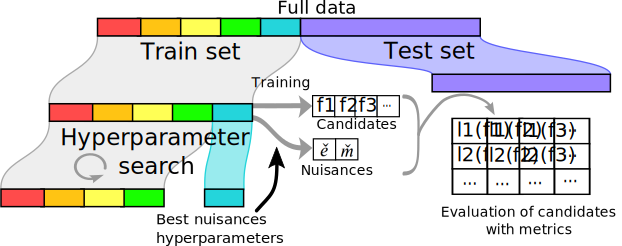
\includegraphics[width=0.9\linewidth]{img/chapter_5/estimation_procedure_causal_selection_procedure.png}
  \caption{Estimation procedure for causal model
    selection.}\label{problem:estimation_procedure:figure}
\end{figure}
%\end{minipage}

\section{Theory: Links between feasible and oracle risks}\label{sec:theory}

We now relate two feasible risks, $\mu \text{-risk}_{IPW}$ and the
$R\text{-risk}$ to the oracle $\tau\text{-risk}$. Both results make
explicit the role of overlap for the performances of causal risks.

These bounds depend on a specific form of residual that we now define: for each potential outcome, $a \in  \{0; 1\}$, the variance conditionally on $x$
is \citep{shalit_estimating_2017}:
\begin{equation*}\label{eq:residuals}
  \sigma_{y}^{2}(x ; a) \overset{\text{def}}{=}
  \int_{y}\left(y-\mu_{a}(x)\right)^{2} p(y \mid x=x ; A=a) \, d y
\end{equation*}
Integrating over the population, we get the Bayes squared error:
$\sigma^2_{B}(a) = \int_{\mathcal X} \sigma_y^2(x;a) p(x)dx$
and its propensity weighted version:
$\tilde{\sigma}^2_{B}(a) = \int_{\mathcal X}\sigma_y^2(x;a)\,  p(x;
  a)\,dx$. In case of a purely deterministic link between the
covariates, the treatment, and the outcome, these residual terms are null.


\subsection{Upper bound of $\tau\text{-risk}$ with $\mu\text{-risk}_{IPW}$}%
\label{theory:mu_risk_ipw_bound}%

\begin{proposition}[Upper bound with $\mu \text{-risk}_{IPW}$
  ]\label{theory:prop:mu_risk_ipw_bound}
  \citep{johansson2022generalization} Given an outcome model $f$, let a
  weighting function $w(x; a) = \frac{a}{e(x)} + \frac{1-a}{1-e(x)}$ as the
  Inverse Propensity Weight. Then, under overlap (assumption
  \ref{assumption:overlap}), we have:
  \begin{equation*}
    \tau\text{-risk}(f) \leq \; 2 \, \mu\text{-risk}_{IPW}(w, f)
    - 2 \, \big(\sigma^2_{B}(1) +  \sigma^2_{B}(0)\big)
  \end{equation*}
\end{proposition}
This result has been derived in previous work
\citep{johansson2022generalization}. It links $\mu\text{-risk}_{IPW}$ to
the squared residuals of each population. For completeness, we provide the proof in \ref{apd:proofs}.

The upper-bound comes from the triangular inequality applied to the residuals of
both populations. The two quantities are equal when the
absolute residuals on treated and untreated populations are equal on the
whole covariate space:
$\forall x \in \mathcal X, |\mu_1(x) - f(x, 1)| = |\mu_0(x) - f(x, 0)|$.
The main difference between the oracle $\tau \text{-risk}$ and the
reweighted mean squared error, $\mu\text{-risk}_{IPW}$, comes from heterogeneous
residuals between populations.
% These quantities are difficult to characterize as
%they are linked both to the estimator and to the data distribution.
%
This bound shows that minimizing the $\mu\text{-risk}_{IPW}$ helps to
minimize the $\tau\text{-risk}$, which leads to
interesting optimization procedures \citep{johansson2022generalization}. However, there is no
guarantee that this bound is tight, which makes it fragile for model
selection.

Assuming strict overlap (probability of all individuals being treated or not
bounded away from 0 and 1 by $\eta$, \ref{background:causal_assumptions}), the
above bound simplifies into a looser one involving the usual mean squared error:
$\tau\text{-risk}(f)\leq \frac{2}{\eta}\, \mu\text{-risk}(f) -  2 \, \big(\sigma^2_{B}(1) +  \sigma^2_{B}(0)\big)$. For weak overlap (propensity scores not bounded far from 0
or 1), this bound is very loose (as shown in Figure \ref{fig:toy_example})
and is not appropriate to discriminate between models with close performances.

%\md{Lower bound: I think that there is no lower bound of the tau-risk with the
%mu-risk. That means that we can have a mu risk of 0 wheras the taurisk is
%non-null. Todo for myself: develop an example with overfitted 1NN on the
%observed data.}

\subsection{Reformulation of the $R\text{-risk}$ as reweighted $\tau\text{-risk}$}%
\label{theory:r_risk_rewrite}%

We now derive a novel rewriting of the $R\text{-risk}$, making explicit its link
with the oracle $\tau \text{-risk}$.

\begin{proposition}[$R \text{-risk}$ as reweighted
    $\tau\text{-risk}$]\label{theory:prop:r_risk_rewrite} Given an outcome model
  $f$, its $R\text{-risk}$ appears as weighted version of its $\tau\text{-risk}$
  (Proof in \ref{apd:proofs:r_risk_rewrite}):
  \begin{align}
    R\text{-risk}^*(f) & = \int_{x} e(x)\big(1-e(x)\big)\big(\tau(x)-\tau_ {f}(x)\big)^{2} p(x) d x  \quad\; + \tilde{\sigma}_B^2(1) + \tilde{\sigma}_B^{2}(0)
  \end{align}
\end{proposition}

The $R \text{-risk}$ targets the oracle at the cost of an overlap re-weighting
and the addition of the reweighted Bayes residuals, which are independent of
$f$. In good overlap regions the weights $e(x) \big(1-e(x) \big)$ are close to
$\frac{1}{4}$, hence the $R \text{-risk}$ is close to the desired gold-standard
$\tau \text{-risk}$. On the contrary, for units with extreme overlap violation,
these weights go down to zero with the propensity score.

% \begin{remark}[Trivial upper bound] Because $e(x)\leq1$ and $(1-e(x))\leq1$,
%   we see immediately that \begin{equation} R \text{-risk}^* \leqslant
%   \tau{\text{-risk}}+\tilde{\sigma_{B}}(1)^{2}+\tilde{\sigma_{B}}^{2}(0)
%   \end{equation} \end{remark}

% \begin{remark}[Lower bound] Due to strict overlap assumption, \begin{equation}
%   R \text{-risk}^* \geqslant \eta (1 - \eta)
%   \tau{\text{-risk}}-\tilde{\sigma_{B}}(1)^{2}-\tilde{\sigma_{B}}^{2}(0)
%   \end{equation} \end{remark}

% \begin{remark}[Cases of loose upper bounds] Giving a strict overlap assumption
%   $\eta$, we can exhibit for all $C \; st. \; \eta^{-1}>C>1$, simple
%   simulations where: \begin{equation} R \text{-risk}^* \leqslant C \; \eta \;
%   \tau \text{-risk}(f) \quad \end{equation} \end{remark}

\subsection{Interesting special cases}

\paragraph{Randomization special case}\label{remark:rct} If the treatment is
randomized as in RCTs, $p(A=1 \mid X=x) = p(A=1)=p_A$, thus
$\mu\text{-risk}_{IPW}$ takes a simpler form:
\begin{equation*}
  \mu\text{-risk}_{IPW} = \mathbb{E}_{(Y, X, A) \sim \mathcal D}\left[ \Big( \frac{A}{p_A} + \frac{1-A}{1-p_A} \Big) (Y-f(X ; A))^2 \right]
\end{equation*}
However, we still can have large differences
between $\tau\text{-risk}$ and $\mu\text{-risk}_{IPW}$ coming from heterogeneous
errors between populations as noted in Section \ref{theory:mu_risk_ipw_bound}
and shown experimentally in \citet{schuler_comparison_2018} and our
results below.

Concerning the $R\text{-risk}$, replacing $e(x)$ by its randomized value $p_A$
in Proposition \ref{theory:prop:r_risk_rewrite} yields the oracle
$\tau\text{-risk}$ up to multiplicative and additive constants:
\begin{equation*}
  R\text{-risk} = p_A \, (1-p_A) \, \tau\text{-risk} \;+\; (1 - p_A) \,\sigma_B^2(0) \;+\; p_A \sigma_B^2(1)
\end{equation*}
Thus, selecting estimators with $R\text{-risk}^*$ in
randomized setting controls the $\tau\text{-risk}$. This explains
the strong performances of $R\text{-risk}$ in randomized setups
\citep{schuler_comparison_2018} and is a strong argument to use it
to estimate heterogeneity in RCTs.

\paragraph{Oracle Bayes predictor}\label{remark:bayes_oracle} If we
have access to the oracle Bayes predictor for the outcome ie.~$f(x,
  a)=\mu(x, a)$, then all risks are equivalent up to the residual variance:
\begin{equation}
  \tau\text{-risk}(\mu) = \mathbb E_{X\sim p(X)}[(\tau(X) - \tau_{\mu}(X))^2] = 0
\end{equation}
\begin{align}
  \mu\text{-risk}(\mu) & = \mathbb E_{(Y, X, A) \sim p(Y;X;A)}[\big( Y - \mu_A(X)\big)^2] \\
                       & = \int_{\mathcal X, \mathcal A}
  \,\varepsilon(x,a)^2 p(a \mid x) \,p(x) \,dx\,da  \leq \sigma_B^{2}(0) + \sigma_B^{2}(1)
\end{align}
\begin{equation}
  \mu\text{-risk}_{IPW}(\mu) = \sigma_B^{2}(0) + \sigma_B^{2}(1)  \quad \text{from Lemma \ref{apd:proofs:mu_risk_ipw_link_mu}}
\end{equation}
\begin{equation}
  R\text{-risk}(\mu) = \tilde{\sigma}_B^{2}(0) + \tilde{\sigma}_B^{2}(1)
  \leq \sigma_B^{2}(0) + \sigma_B^{2}(1)  \quad  \text{from Proposition \ref{theory:prop:r_risk_rewrite}}%\notag
\end{equation}

Thus, differences between causal risks only matter in finite sample regimes.
Universally consistent learners converge to the Bayes risk in asymptotic
regimes, making all model selection risks equivalent. In practice however,
choices must be made in non-asymptotic regimes.



\section{Empirical Study}\label{sec:empirical_study}

%We now explore empirically the behavior of these different causal selection
%metrics.
%\subsection{Causal metrics under evaluation}

We evaluate the following causal metrics, oracle and feasible
versions, presented in Table
\ref{tab:evaluation_metrics}:\\
$\widehat{\mu\text{-risk}}_{IPW}^*$,
$\widehat{R\text{-risk}}^*$,
$\widehat{U\text{-risk}}^*$,
$\widehat{\tau\text{-risk}_{IPW}}^*$,
$\widehat{\mu\text{-risk}}$,
$\widehat{\mu\text{-risk}}_{IPW}$,
$\widehat{R\text{-risk}}$,
$\widehat{U\text{-risk}}$,
$\widehat{\tau\text{-risk}_{IPW}}$.
We benchmark the metrics in a variety of settings:
many different simulated data generation
processes and three semi-simulated datasets \footnote{Scripts for the simulations and the selection procedure are available at
  \url{https://github.com/soda-inria/caussim}.
}.

\subsection{Caussim: Extensive simulation settings}\label{subsec:simulations}

\paragraph{Data Generation}

We use simulated data, on which the ground-truth causal effect is known. Going
beyond prior empirical studies of causal model selection
\citep{schuler_comparison_2018,alaa_validating_2019}, we use many
generative processes, to reach more general conclusions (as discussed
in \ref{apd:results:fig:seed_effect}).

We generate the response functions using random bases. Basis extension methods
are common in biostatistics, \emph{eg} functional regression with splines
\citep{howe_splines_2011, perperoglou_review_2019}. By allowing the function to
vary at specific knots, they give flexible non-linear models. We use random approximation of Radial Basis Function (RBF) kernels
\citep{rahimi_random_2008} to generate the response functions. RBF use the same
process as polynomial splines but replace polynomial by Gaussian kernels. Unlike
polynomials, Gaussian kernels have decreasing influences in the input space.
This avoids unrealistic divergences of the response surfaces at the
ends of the feature space.

The number of basis functions --\emph{ie. knots}--, controls the complexity of
the ground-truth response surfaces and treatment. We first use this process to
draw the non-treated response surface $\mu_0$ and the causal effect $\tau$. We
then draw the observations from a mixture two Gaussians, for the treated and non
treated. We vary the separation between the two Gaussians to control the
overlap between treated and non-treated populations, an important parameter
for causal inference (related to $\eta$ in section
\ref{theory:mu_risk_ipw_bound}). Finally, we generate observed outcomes
adding Gaussian noise yielding a dataset as plotted in Figure \ref{fig:simulation_examples}. We generate 1\,000 of such datasets, with
uniformly random overlap parameters. Details in
\ref{apd:experiments:generation}.

\captionsetup[sub]{font=large, labelfont={bf,sf}}%

\begin{figure}[b!]
  \begin{minipage}{0.3\textwidth}
    \caption{Example of the simulation setup in the input space with two
      knots --\emph{ie.}basis functions. The top panel
      shows the observations in feature space, while the bottom panel displays the
      two response surfaces on a 1D cut along the black lines drawn on
      the top panel.}
    \label{fig:simulation_examples}
  \end{minipage}
  \hfill
  \begin{minipage}{0.65\textwidth}
    \centering
    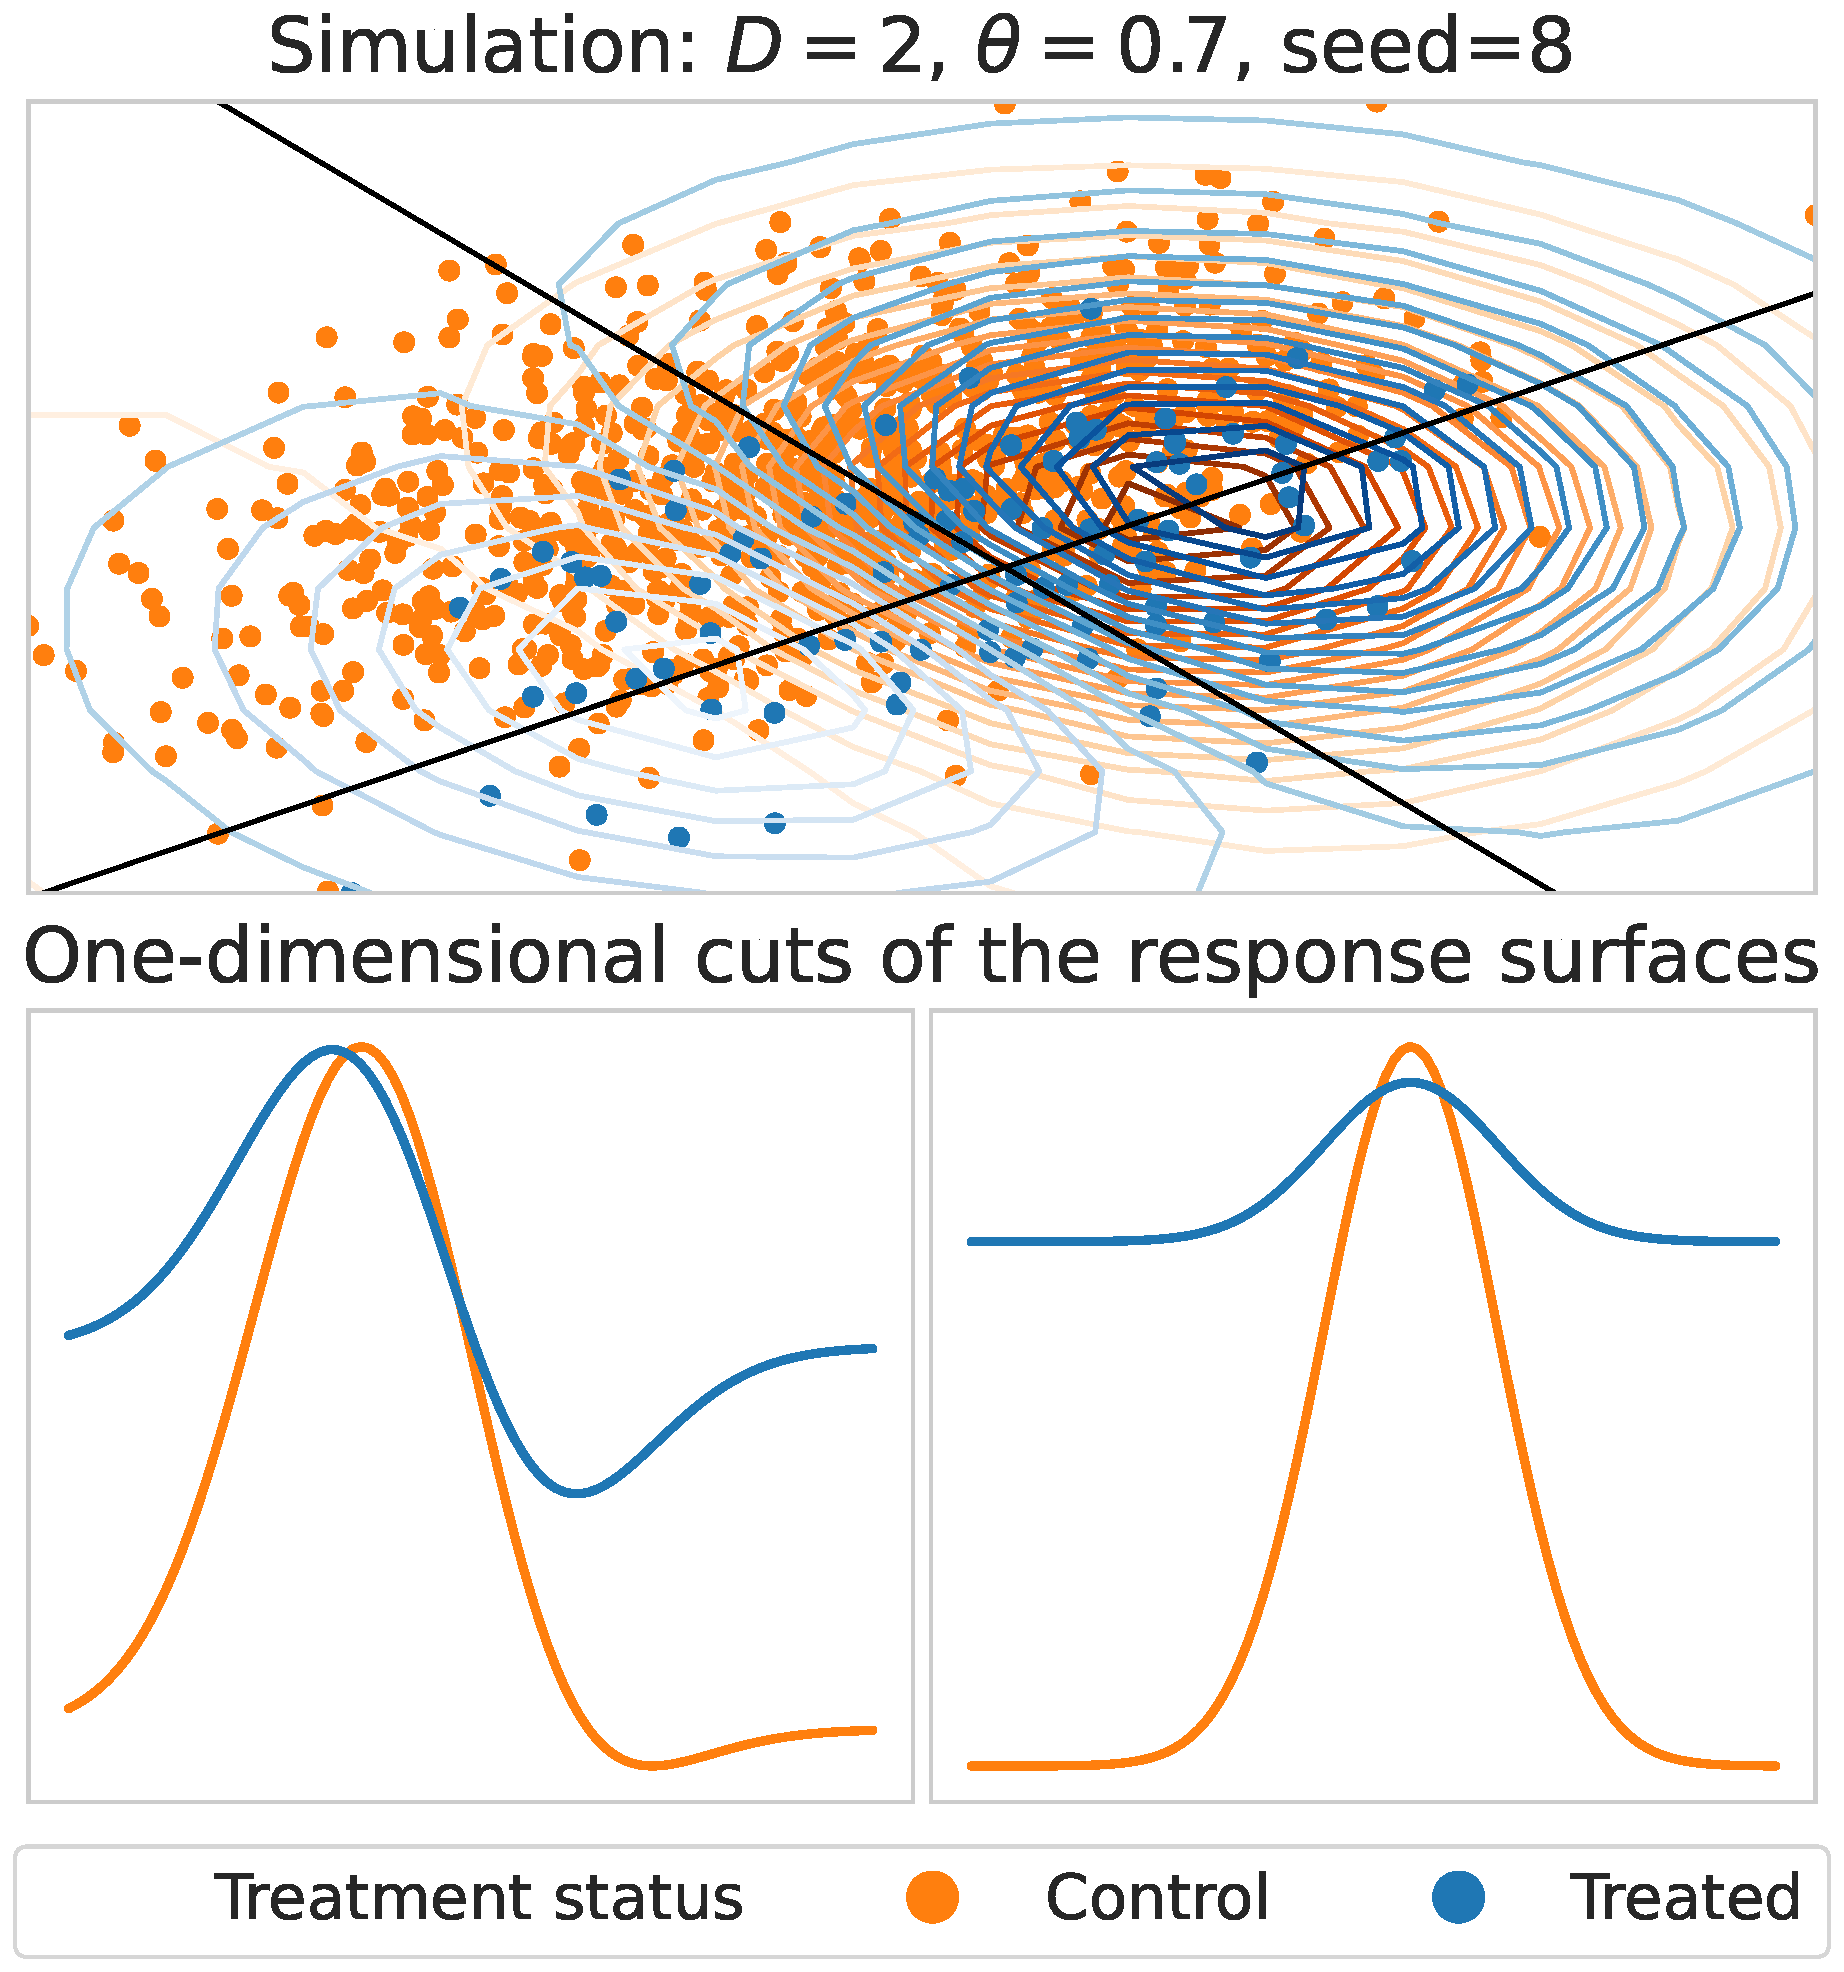
\includegraphics[width=0.8\linewidth]{img/chapter_5/caussim_example_rs_gaussian=8_rs_rotation=8_ntv=0.37_D=2_overlap=0.7_p_A=0.1.pdf}
  \end{minipage}
\end{figure}


\paragraph{Family of candidate estimators}

We test model selection on a family of candidate estimators that
approximate imperfectly the data-generating process. To build such an
estimator, we first use a RBF expansion
similar to the one used for data generation.
We choose two random knots and apply a transformation of the raw data features
with a Gaussian kernel. This step
is referred as the featurization. Then, we fit a linear regression on
these
transformed features. We consider two ways of combining these steps for outcome
mode; we use common nomenclature \citep{kunzel_metalearners_2019,shen2023rctrep} to refer
to these different meta-learners that differ on how
they model, jointly or not, the treated and the non treated:
\begin{itemize}
  \item SLearner: A single learner for both population, taking the treatment as
        a supplementary covariate.

  \item SftLearner: A single set of basis functions is sampled at random for both
        populations, leading to a given feature space used to model both the treat and
        the non treated, then two
        separate different regressors are fitted on this shared representation.
  \item TLearner: Two completely different learners for each population, hence
        separate feature representations and regressors.
\end{itemize}

We do not include more elaborated meta-learners such as R-learner
\citep{nie_quasioracle_2017} or X-learner
\citep{kunzel_metalearners_2019}. Our goal is not to have the best possible
learner but to have a variety of sub-optimal learners to compare the
different causal metrics. For the same reason, we did not include more powerful
outcome models such as random forests or boosting trees.

For the regression step, we fit a Ridge regression on the transformed features
with 6 different choices of the regularization parameter $\lambda \in [10^{-3},
    10^{-2}, 10^{-1}, 1, 10^{1}, 10^{2}]$, coupled with a TLearner or a SftLearner.
We sample 10 different random basis for learning and
featurization yielding a family $\mathcal F$ of 120 candidate estimators.
%

\subsection{Semi-simulated datasets}\label{subsec:causal_model_selection:semi_simulated}

\paragraph{Datasets}

We also use classic benchmarks of the causal-inference
literature, semi-simulated data adding a known synthetic causal effect to real --non synthetic-- covariate:
\begin{description}
  \item[ACIC 2016] \citep{dorie_automated_2019}: The dataset is based on the
    Collaborative Perinatal Project \citep{niswander_women_1972}, a RCT
    studying infants’
    developmental disorders. The initial intervention was a child’s birth
    weight $(A = 1 \text{ if weight} < 2.5 kg)$, and outcome was the child’s
    IQ after a follow-up period. The study contained $N=4\,802$ data
    points with $D=55$ features (5 binary, 27 count data, and 23
    continuous). They simulated 77 different setups varying parameters
    for treatment and response models, overlap, and interactions between treatment and
    covariates \footnote{Original R code available at
      \url{https://github.com/vdorie/aciccomp/tree/master/2016}
      to generate 77 simulations settings.}. We used 10 different seeds for
    each setup, totaling 770 dataset instances.

  \item[ACIC 2018] \citep{shimoni_benchmarking_2018}: Starting from data
    from the Linked Births and Infant Deaths Database (LBIDD)
    \citep{macdorman_infant_1998} with $D=177$ covariates, treatment and
    outcome models are simulated with complex models to reflect
    different scenarios. The data do not provide the true propensity
    scores, so we evaluate only feasible metrics, which do not require this
    nuisance parameter. We used all 432 datasets\footnote{Using the scaling part of the data, from
      \href{https://github.com/IBM-HRL-MLHLS/IBM-Causal-Inference-Benchmarking-Framework}{github.com/IBM-HRL-MLHLS/IBM-Causal-Inference-Benchmarking-Framework}} of size $N=5\,000$.


  \item[Twins] \citep{louizos_causal_2017}: It is an augmentation of
    real data on twin births and mortality rates
    \citep{almond_costs_2005}. There are $N=11\,984$ samples (pairs of twins),
    and $D=50$ covariates\footnote{We obtained the dataset from
      \href{https://github.com/AMLab-Amsterdam/CEVAE/tree/master/datasets/TWINS}{https://github.com/AMLab-Amsterdam/CEVAE/tree/master/datasets/TWINS}}, The outcome is the mortality and the treatment is the
    weight of the heavier twin at birth. This is a "true" counterfactual dataset
    \citep{curth_really_2021} in the sense that we have
    both potential outcomes with each twin. They simulate the treatment with a
    sigmoid model based on GESTAT10 (number of gestation weeks before birth) and x
    the 45 other covariates:
    \begin{align}
      \mathbf{t}_{i} & \mid \mathbf{x}_{i}, \mathbf{z}_{i} \sim
      \operatorname{Bern}\left(\sigma\left(w_{o}^{\top}
      \mathbf{x}+w_{h}(\mathbf{z} / 10-0.1)\right)\right)       \\ & \text{with} \;
      w_{o} \sim \mathcal{N}(0,0.1 \cdot I),\; w_{h} \sim \mathcal{N}(5,0.1) \nonumber
    \end{align}
    We add a non-constant slope in the
    sigmoid to control the overlap between
    treated and control populations.
    We sampled uniformly 1\,000 different overlap parameters between 0 and
    2.5, totaling 1\,000 dataset instances. Unlike the previous datasets,
    only the overlap varies for these instances. The response surfaces are
    set by the original outcomes.
\end{description}

\paragraph{Family of candidate estimators}

For these three datasets, the family of candidate estimators are gradient
boosting trees for both the response surfaces and the treatment
\footnote{Scikit-learn regressor,
  \href{https://scikit-learn.org/stable/modules/generated/sklearn.ensemble.HistGradientBoostingRegressor.html}{HistGradientBoostingRegressor},
  and classifier,
  \href{https://scikit-learn.org/stable/modules/generated/sklearn.ensemble.HistGradientBoostingClassifier.html}{HistGradientBoostingClassifier}.}
with S-learner, learning rate
in $\{0.01, 0.1, 1\}$, and maximum number of leaf nodes in $\{25, 27, 30, 32,
  35, 40\}$ resulting in a family of size 18.

\paragraph{Nuisance estimators}

Drawing inspiration from the TMLE literature that uses combination of flexible
machine learning methods \citep{schuler_targeted_2017}, we use as models
for the nuisances $\check e$ (respectively $\check m$) a form of meta-learner: a
stacked estimator of ridge and boosting classifiers (respectively
regressions). We select hyper-parameters with randomized search on a validation set
$\mathcal{V}$ and keep them fix for model selection
(\ref{apd:experiments:nuisances_hp} lists hyperparameters). As extreme inverse
propensity weights induce high variance, we use clipping
\citep{swaminathan_counterfactual_2015, ionides_truncated_2008} to bound
$min(\check e, 1-\check e)$ away from 0 with a fixed $\eta=10^{-10}$, ensuring
strict overlap for numerical stability.


%\paragraph{Model selection procedure}\label{semi_simulated:selection_procedure}

%We used the same training procedure procedure as in
%\ref{paragraph:selection_procedure} (Details in supp.~mat.
%\ref{apd:selection_procedure_acic}).

\subsection{Measuring overlap between treated and non treated}%
\label{subsec:causal_model_selection:measuring_overlap}%

%\idea{Overlap is important but not easily measurable}
Good overlap between treated and control population is
crucial for causal inference as it is required by the positivity assumption
\ref{assumption:overlap}. It is often assessed by
comparing visually population distributions (as in Figure
\ref{fig:toy_example}) or computing standardized difference on each
feature
\citep{austin_introduction_2011,austin2015moving}. While these methods are
useful to decide if positivity holds, they do not yield a
single measure. Rather, we compute the divergence
between the population covariate distributions $\mathbb P(X|A=0)$ and $\mathbb
  P(X|A=1)$
\citep{damour_overlap_2020,johansson2022generalization}. We introduce the
Normalized Total Variation (NTV), a divergence based on the sole propensity
score (see \ref{apd:motivation_ntv}).

\begin{figure}[!b]
  \centering
  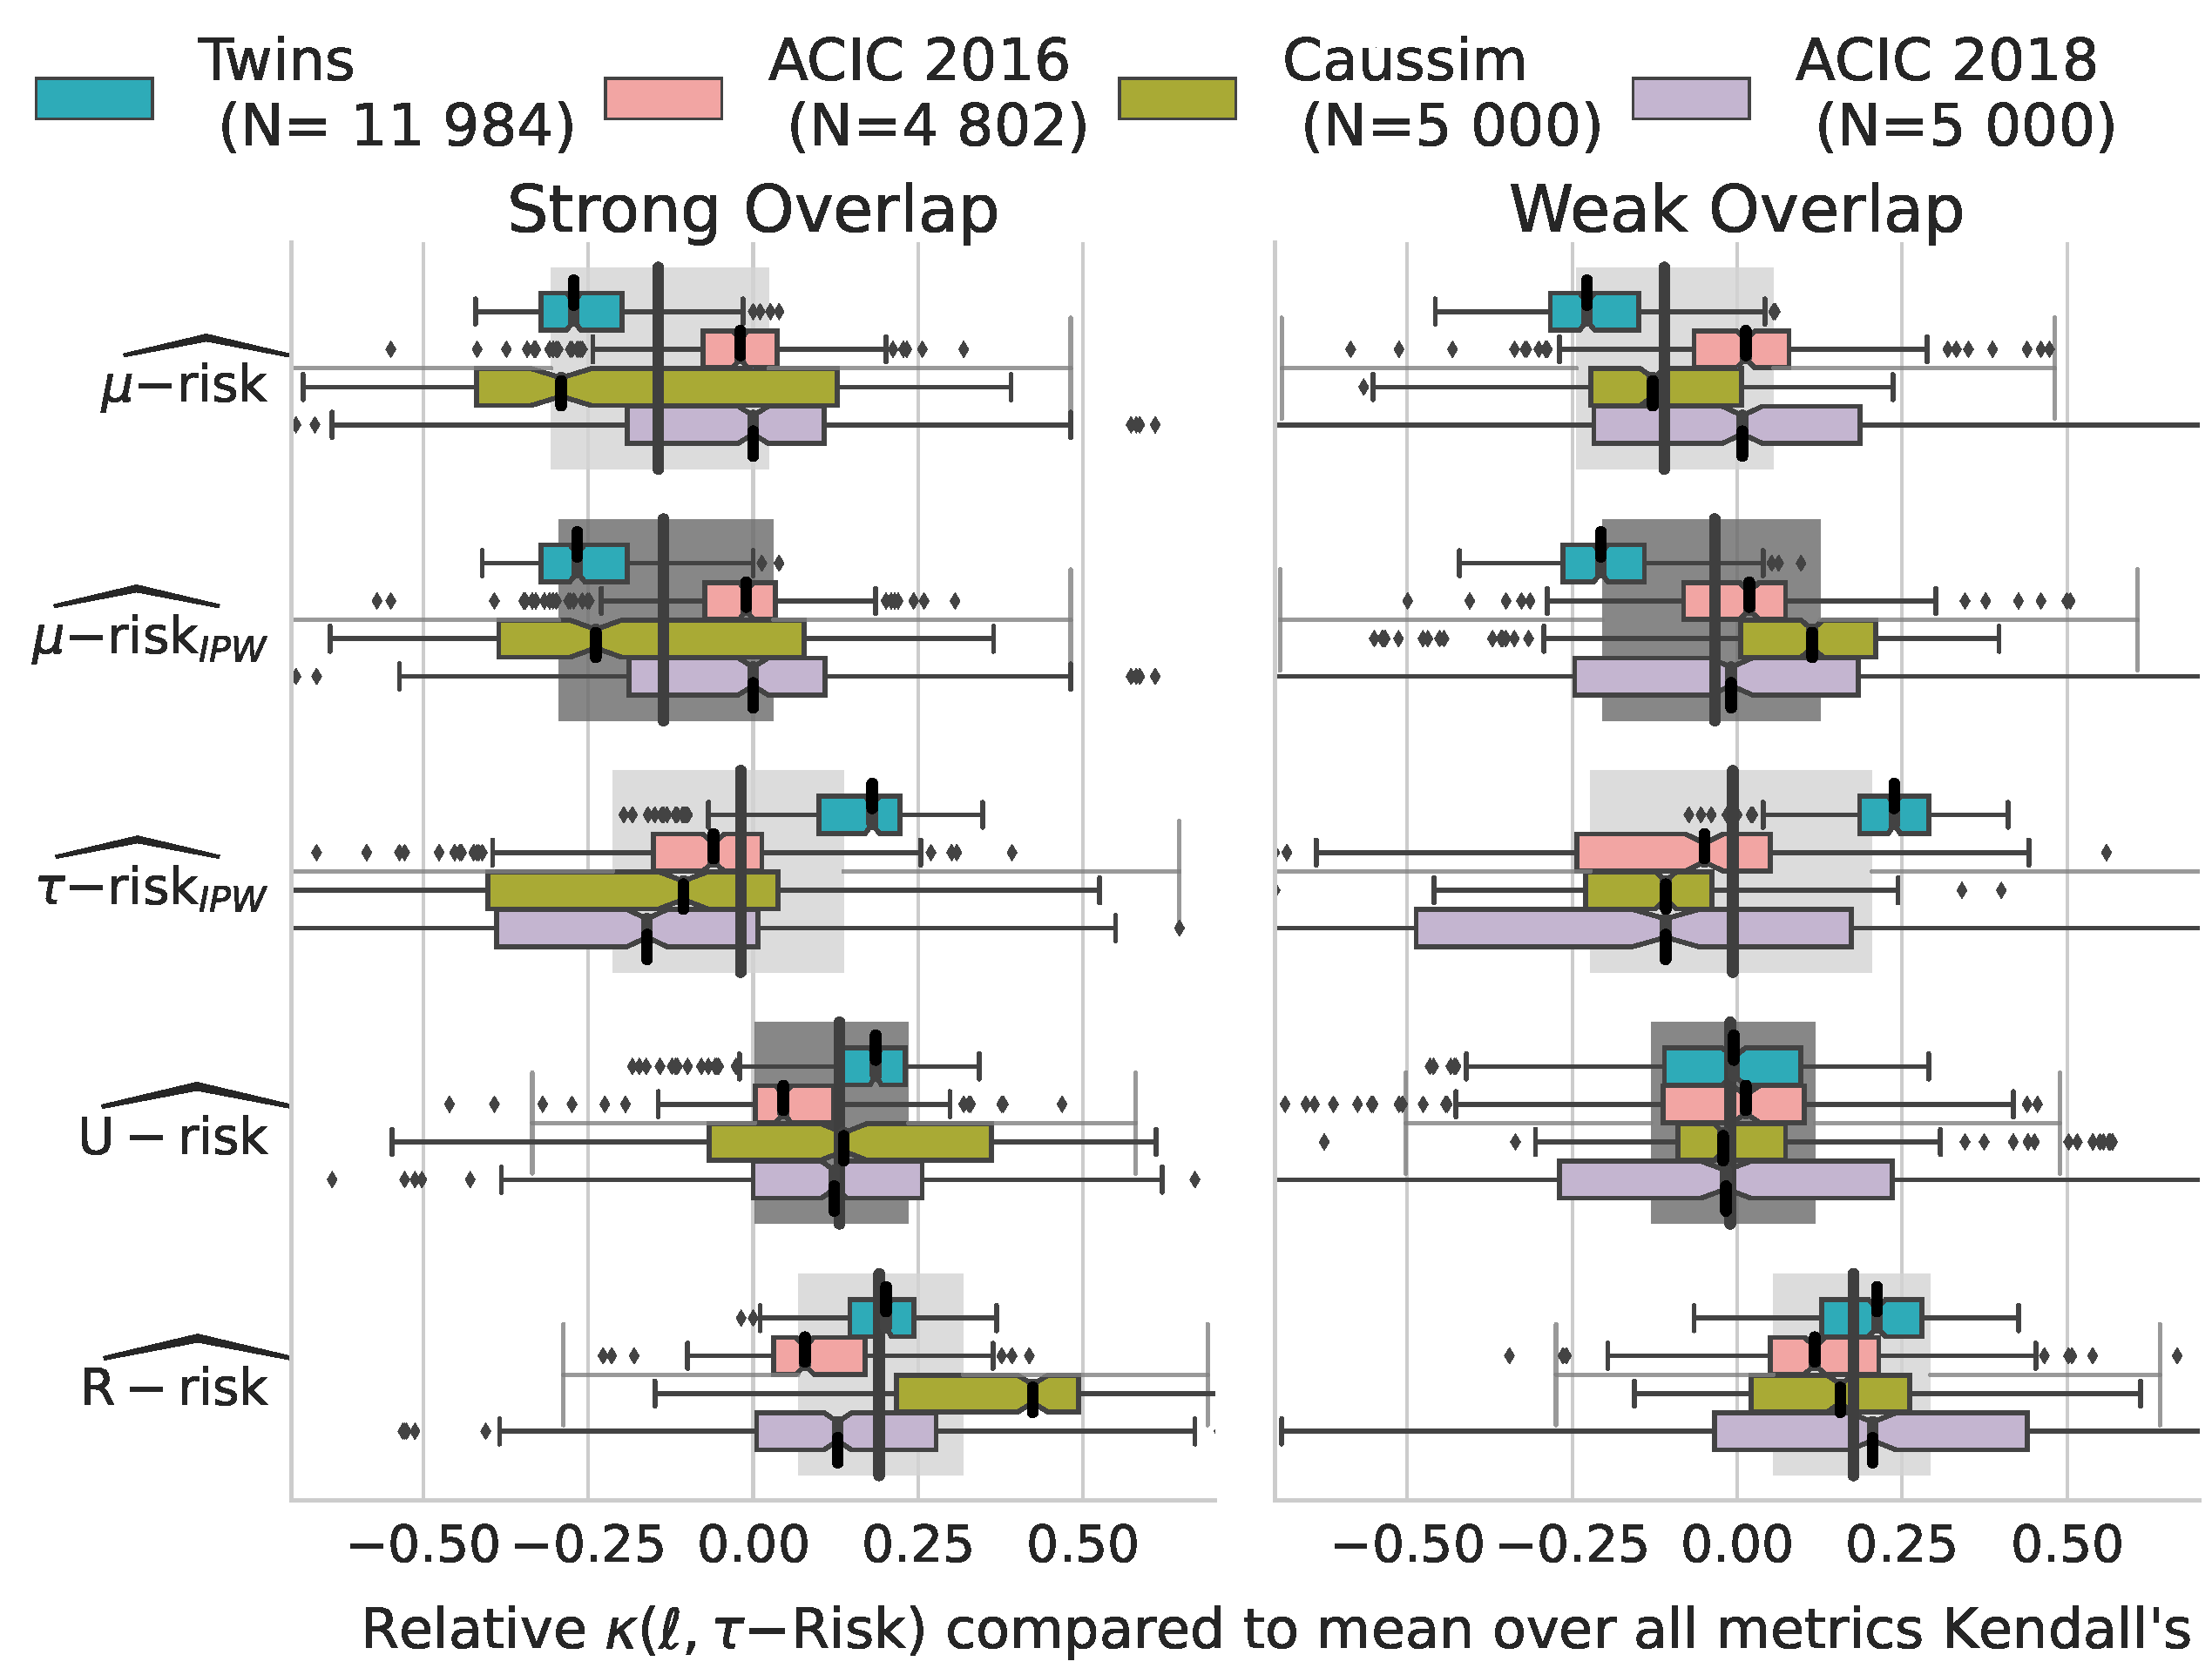
\includegraphics[width=0.9\linewidth]{img/chapter_5/_1_r_risk_domination_r_risk_domination__ref_metric_mean_risks_by_Dataset_feasible_only.pdf}
  %\hfill
  \caption{\textbf{The $R$-risk is the best metric}: Relative Kendall's $\tau$ agreement with $\tau\text{-risk}$.
    Strong and Weak overlap correspond to the first and last tertiles of the overlap distribution measured with
    Normalized Total Variation eq. \ref{eq:ntv}. \ref{apd:experiments:additional_results} presents the same results
    by adding semi-oracle risks in Figure \ref{apd:fig:relative_kendalls_all_datasets_all_metrics}, measured with
    absolute Kendall's in Figure \ref{apd:fig:all_datasets_tau_risk_ranking_agreement} and with $\tau\mathrm{-risk}$
    gains in Figure \ref{apd:all_datasets_normalized_bias_tau_risk_to_best_method}. Table
    \ref{apd:table:relative_kendalls_all_datasets} gives median and
    IQR of the relative Kendall.}\label{fig:relative_kendalls_all_datasets}
\end{figure}

\subsection{Results: factors driving good model selection}%
\label{subsec:causal_model_selection:empirical_results}%

\paragraph{The $R\text{-risk}$ is the best metric}

Each metric ranks differently the candidate models. Figure
\ref{fig:relative_kendalls_all_datasets} shows the agreement between the
ideal ranking of methods given the oracle $\tau\text{-risk}$ and
the different feasible causal metrics. We measure this agreement
with a relative\footnote{To remove the variance
  across datasets (some datasets lead to easier model selection than
  others), we report values for one metric relative to the mean of all
  metrics for a given dataset instance: $\text{Relative} \, \kappa(\ell,\tau\mathrm{{-risk}})=
    \kappa(\ell,\tau\mathrm{{-risk}}) -
    mean_{\ell}\big(\kappa(\ell,\tau\mathrm{{-risk}})\big)$} Kendall tau $\kappa$ (eq.
\ref{eq:kendall_tau}) \citep{kendall_new_1938}.
Given the importance of overlap in
how well metrics approximate the oracle $\tau\text{-risk}$
(\ref{apd:proofs:mu_risk_ipw_bound}), we separate
strong and weak overlap.

Among all metrics, the classical mean squared error (ie. factual
$\mu\text{-risk}$) is worse and reweighting it with propensity score
($\mu\text{-risk}_{IPW}$) does not bring much improvements. The
$R\text{-risk}$, which includes a model of mean outcome and propensity
scores, leads to the best performances. Interestingly, the
$U\text{-risk}$, which uses the same nuisances, deteriorates in weak overlap, probably due to variance
inflation when dividing by extreme propensity scores.

Beyond rankings, the differences in terms of absolute
ability to select the best model are large: The R-risk selects a model
with a $\tau\text{-risk}$ only 1\% higher
than the best
possible candidate for strong overlap on Caussim, but selecting with
the $\mu\text{-risk}$ or $\mu\text{-risk}_{IPW}$ --as per machine-learning
practice-- leads to 10\% excess risk and using $\tau\text{-risk}_{IPW}$
--as in some causal-inference methods \citep{athey2016recursive,gutierrez_causal_2016}--leads to 100\% excess risk
(Figure
\ref{apd:all_datasets_normalized_bias_tau_risk_to_best_method}). Across
datasets, the $R\text{-risk}$ consistently decreases the
risk compared to the $\mu\text{-risk}$:
0.1\% compared to 1\% on ACIC2016,  1\% compared to 20\% on ACIC2018,
and 0.05\% compared to 1\% on Twins.


\paragraph{Model selection is harder for low population
  overlap}

Model selection for
causal inference becomes more and more difficult with increasingly different
treated and control populations
(Figure \ref{fig:all_datasets_overlap_effect_r_risk}). The
absolute Kendall's coefficient correlation with $\tau\text{-risk}$
drops from values around 0.9 (excellent agreement with oracle selection) to 0.6 on
both Caussim and ACIC 2018
(\ref{apd:experiments:additional_results}).

\begin{figure}[h!]
  \begin{minipage}{.35\linewidth}
    \caption{\textbf{Model selection is harder for low population
        overlap}:
      Kendall's $\tau$ agreement with $\tau\text{-risk}$. Strong, medium and Weak overlap
      are the tertiles of the overlap measured with NTV eq. \ref{eq:ntv}. \ref{apd:experiments:additional_results} presents results for all
      metrics in Figure \ref{apd:fig:all_datasets_overlap_effect} in absolute
      Kendall's and continuous overlap values in Figure
        {\ref{apd:fig:all_datasets_tau_risk_ranking_agreement}}.}\label{fig:all_datasets_overlap_effect_r_risk}
  \end{minipage}
  \hfill
  \begin{minipage}{0.6\linewidth}
    \centering
    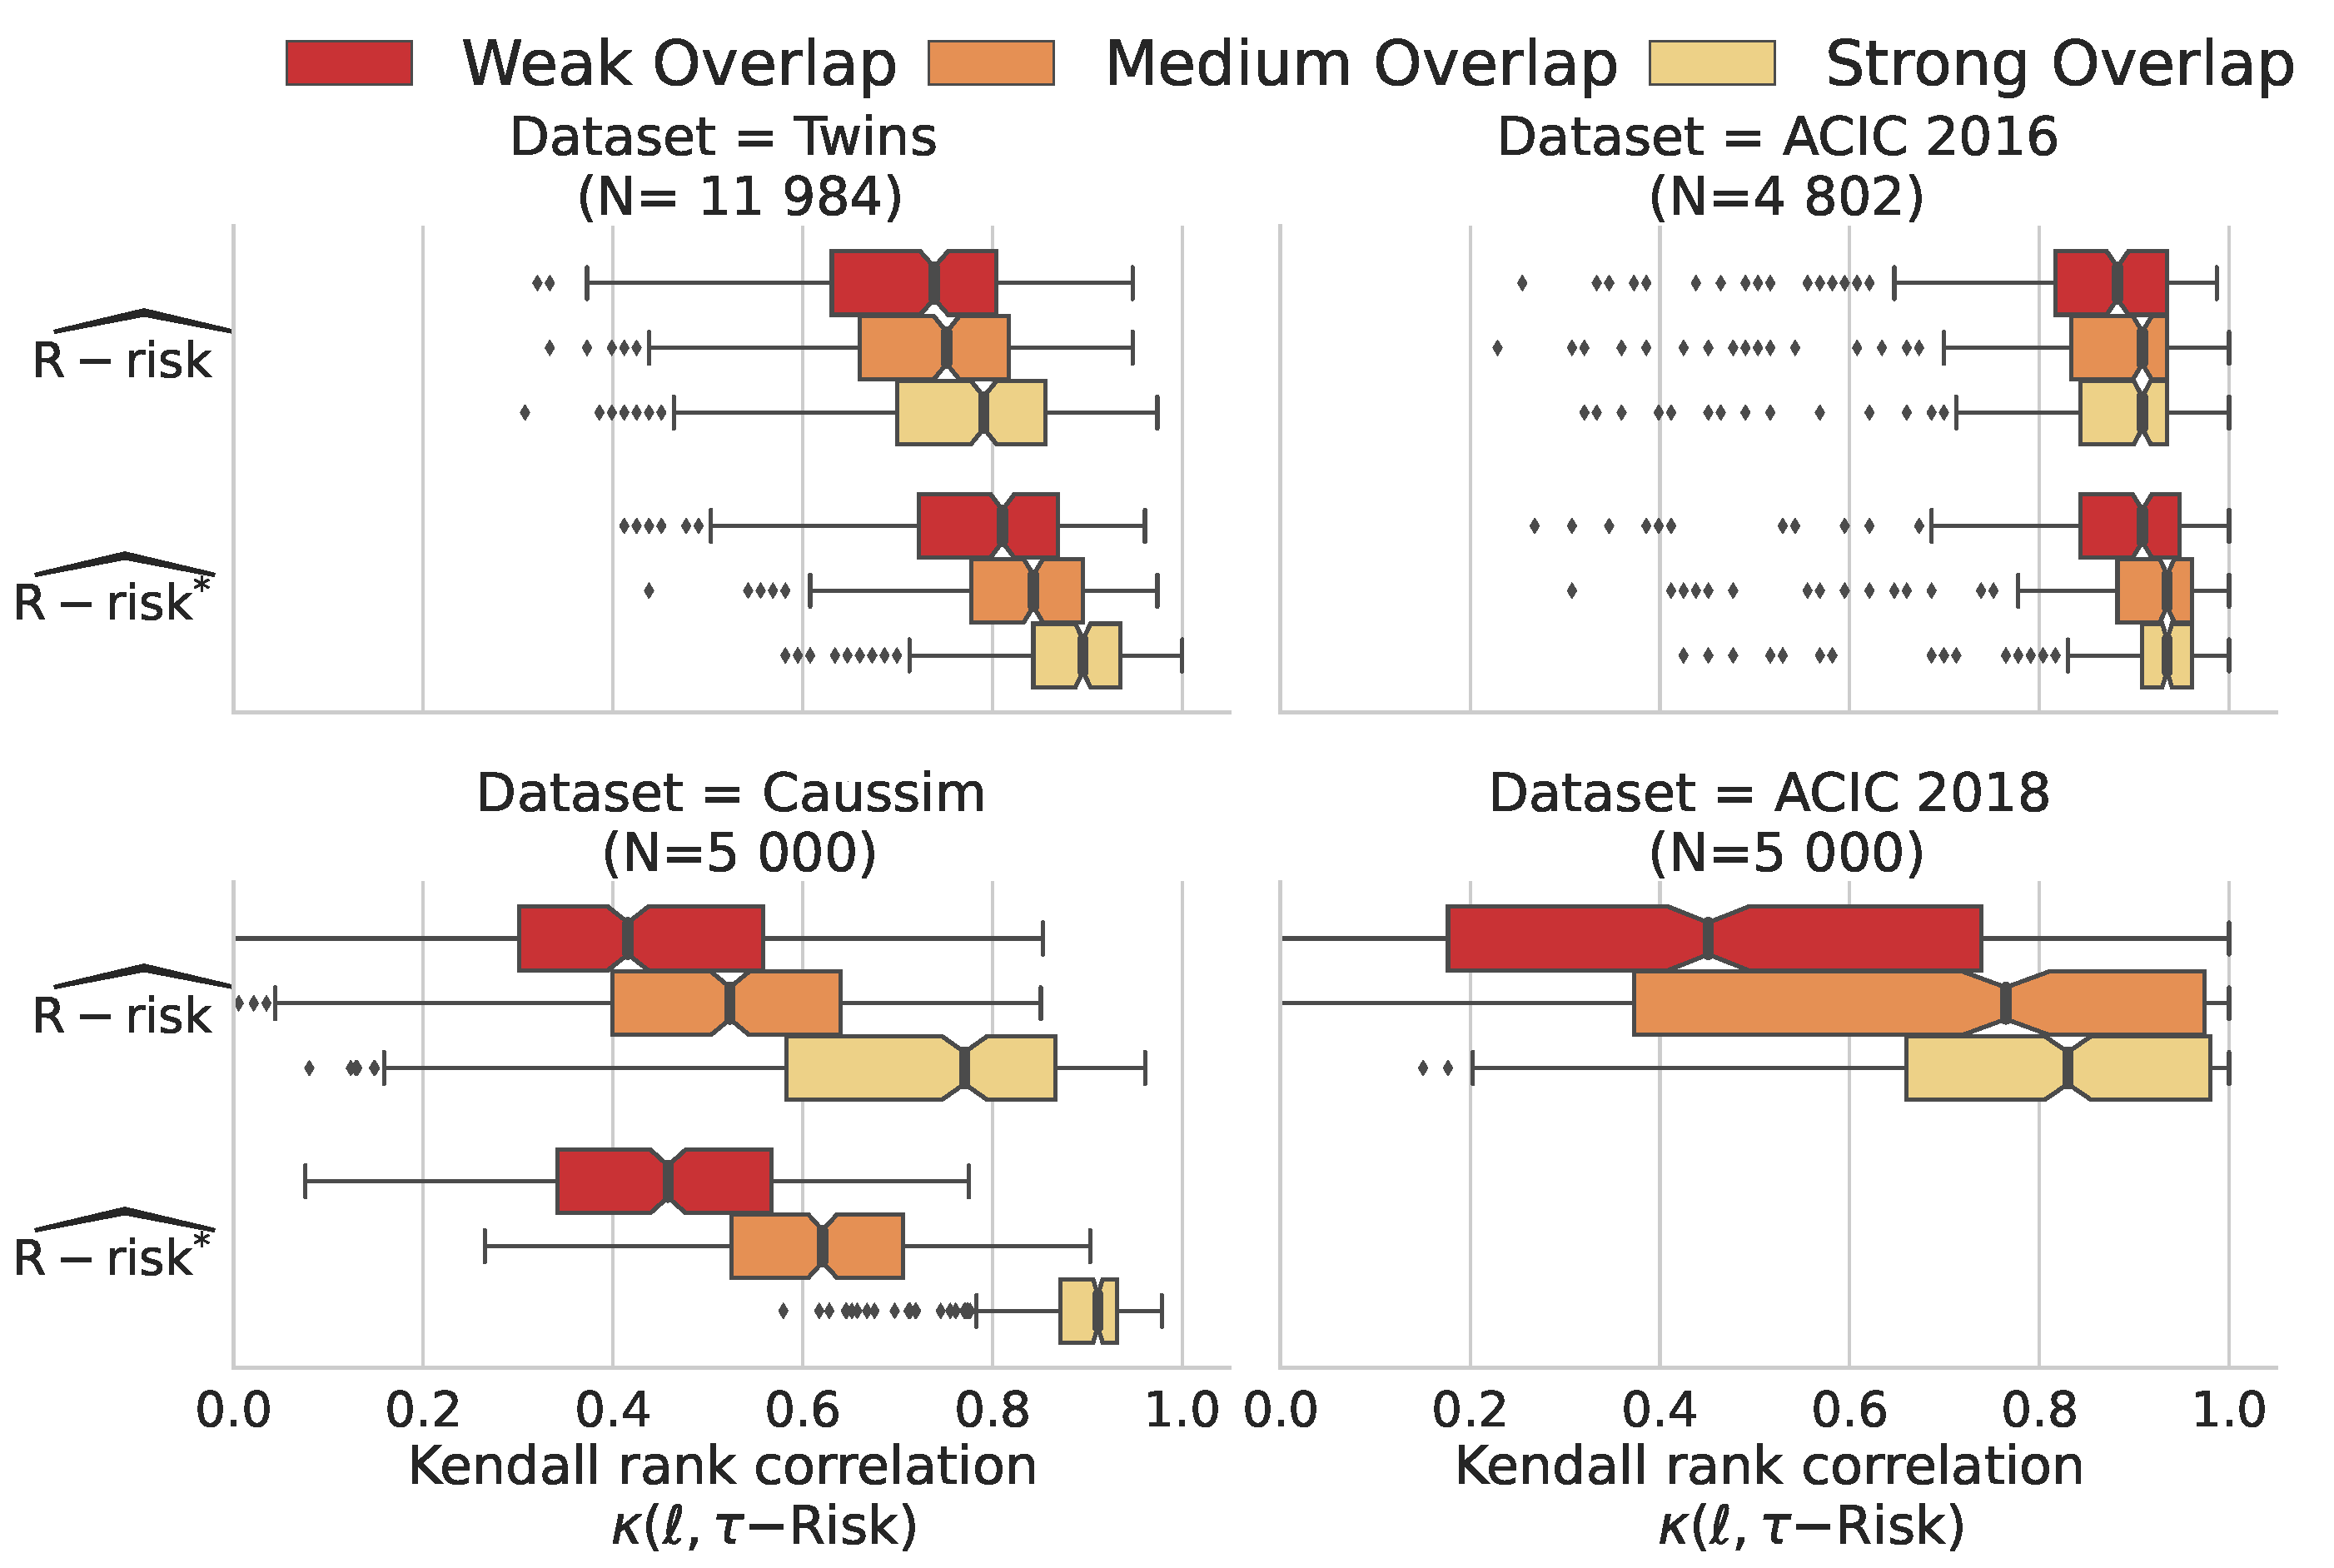
\includegraphics[width=\linewidth]{img/chapter_5/_2_overlap_influence_overlap_by_bin_comparaison_kendall_by_Dataset_r_risk_only.pdf}
  \end{minipage}
\end{figure}

\paragraph{Nuisances can be estimated on the same data as outcome models}

Using the train set $\mathcal{T}$ both to fit the candidate estimator and the
nuisance estimates is a form of double dipping which can lead errors in
nuisances correlated to that of outcome models
\citep{nie_quasioracle_2017}. In theory, these correlations can bias model
selection and, strictly speaking, push
to split out a third separated data set --a ``nuisance set''-- to fit the
nuisance models. The drawback is that it depletes the data available for
model estimation and selection. However, Figure
\ref{fig:procedures_comparison} shows no substantial difference between a procedure with a separated
nuisance set and the simpler shared nuisance-candidate set procedure.

\begin{figure}[!tb]
  \centering
  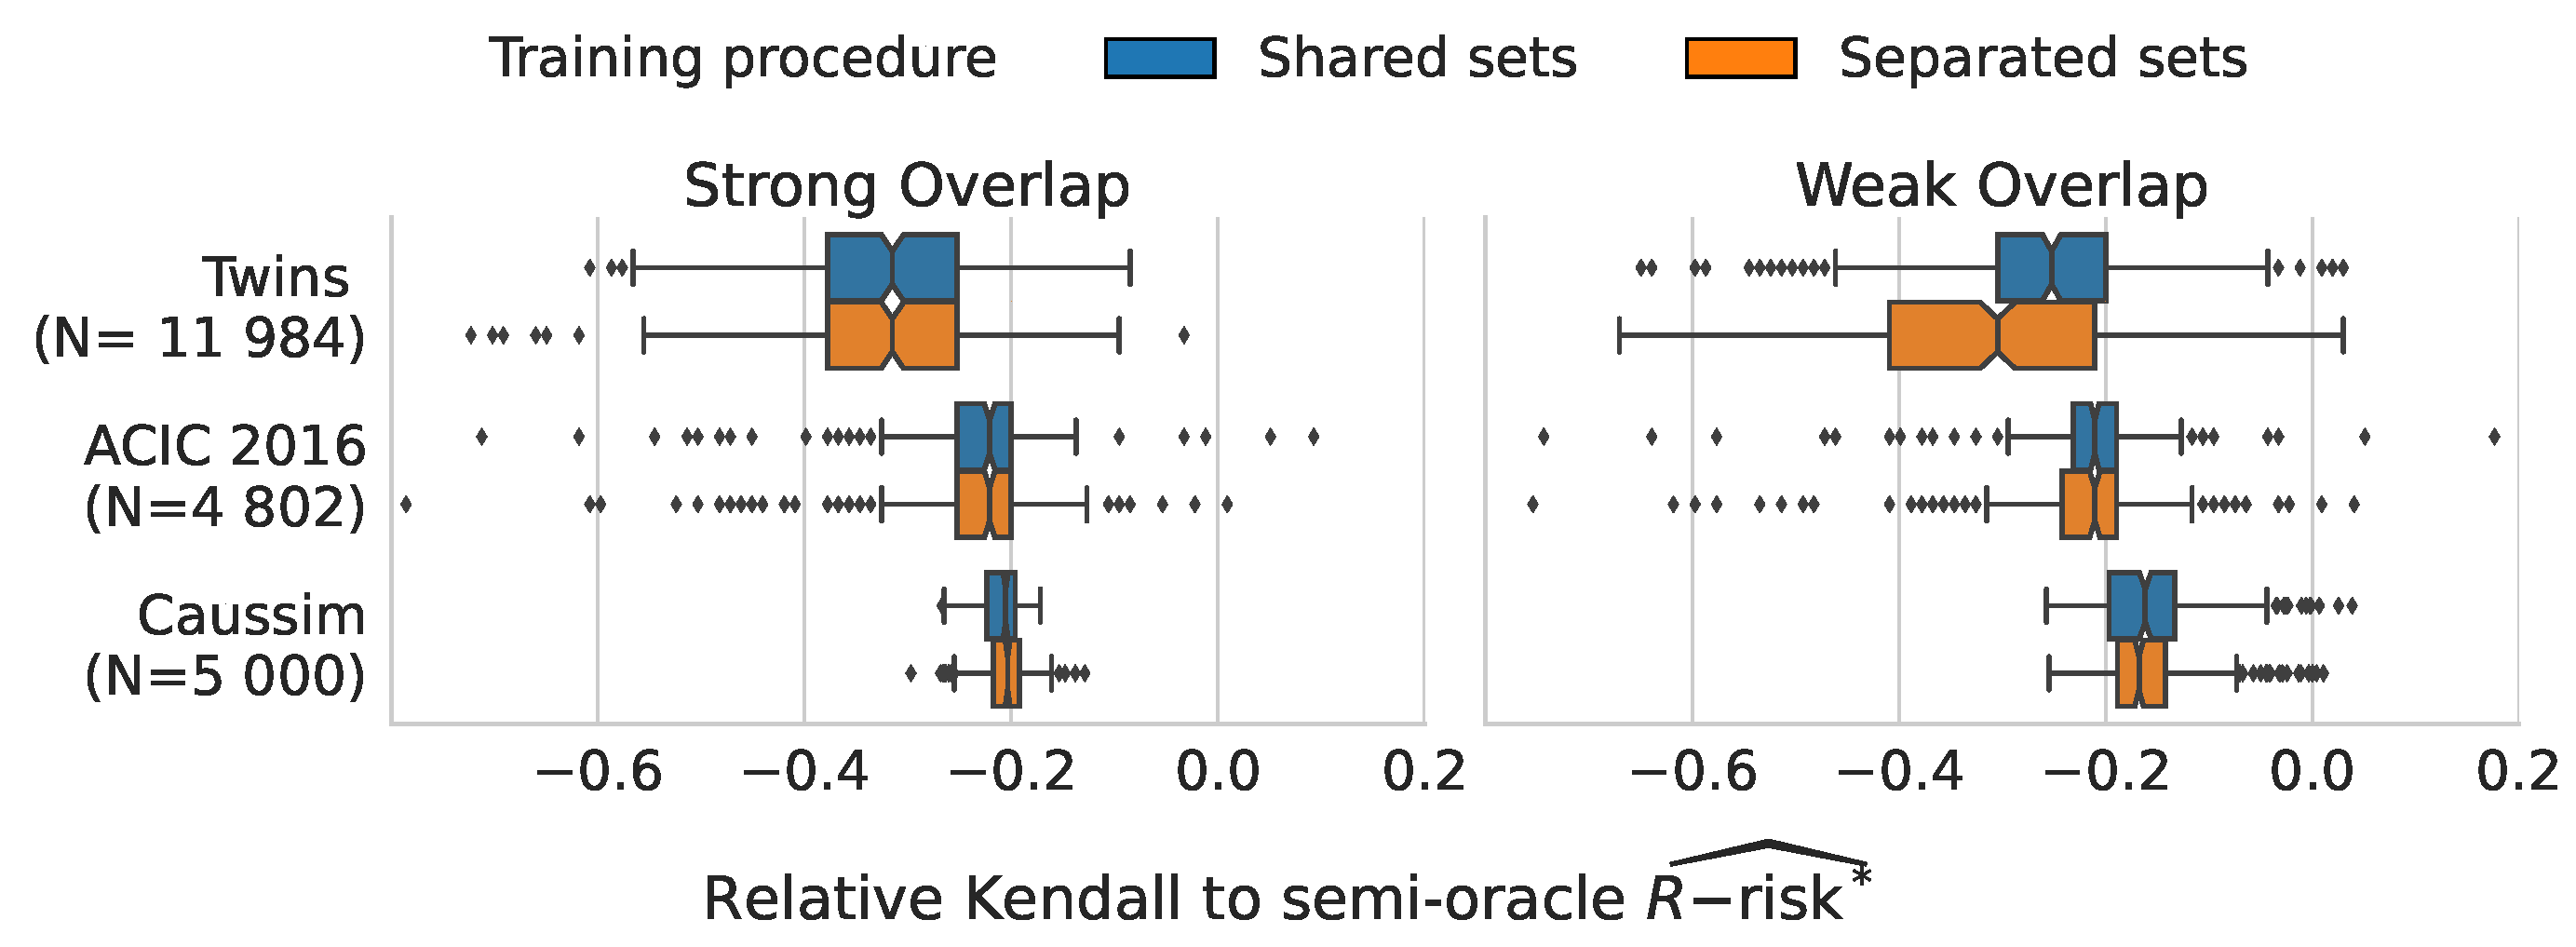
\includegraphics[width=\linewidth]{img/chapter_5/_3_procedure_r_risk_only_3datasets.pdf}
  \caption{\textbf{Nuisances can be estimated on the same data as outcome
      models}: Results for the R-risk are similar between the
    \textcolor{MidnightBlue}{shared
      nuisances/candidate set} and
    the \textcolor{RedOrange}{separated nuisances set} procedures. Figure
    \ref{apd:fig:procedures_comparison_all_metrics} details results for all metrics.}\label{fig:procedures_comparison}
\end{figure}


\paragraph{Stacked models are good overall estimators of nuisances}

For every risk, the oracle version recovers better the best estimator.
However,
stacked nuisances estimators (boosting and linear) lead to feasible
metrics with close performances to the oracles ones: the
corresponding estimators recover well-enough the true nuisances.
One may wonder if simpler models for the nuisance could be useful,
in particular in data-poor settings or when the true models are linear.
Figure \ref{fig:all_datasets_nuisances_comparison} compares causal model
selection estimating nuisances with stacked estimators or linear model.
It comprises the Twins data, where the true propensity model is linear,
and a downsampled version of this data, to study a situation favorable to
linear models. In these settings,
stacked and linear estimations of the nuisances performs equivalently.
Detailed analysis (Figure \ref{apd:fig:nuisances_comparison_twins})
confirms that using adaptive models --as built by
stacking linear models and gradient-boosted trees-- suffices to estimate nuisance.

\begin{figure}[!tb]
  \centering
  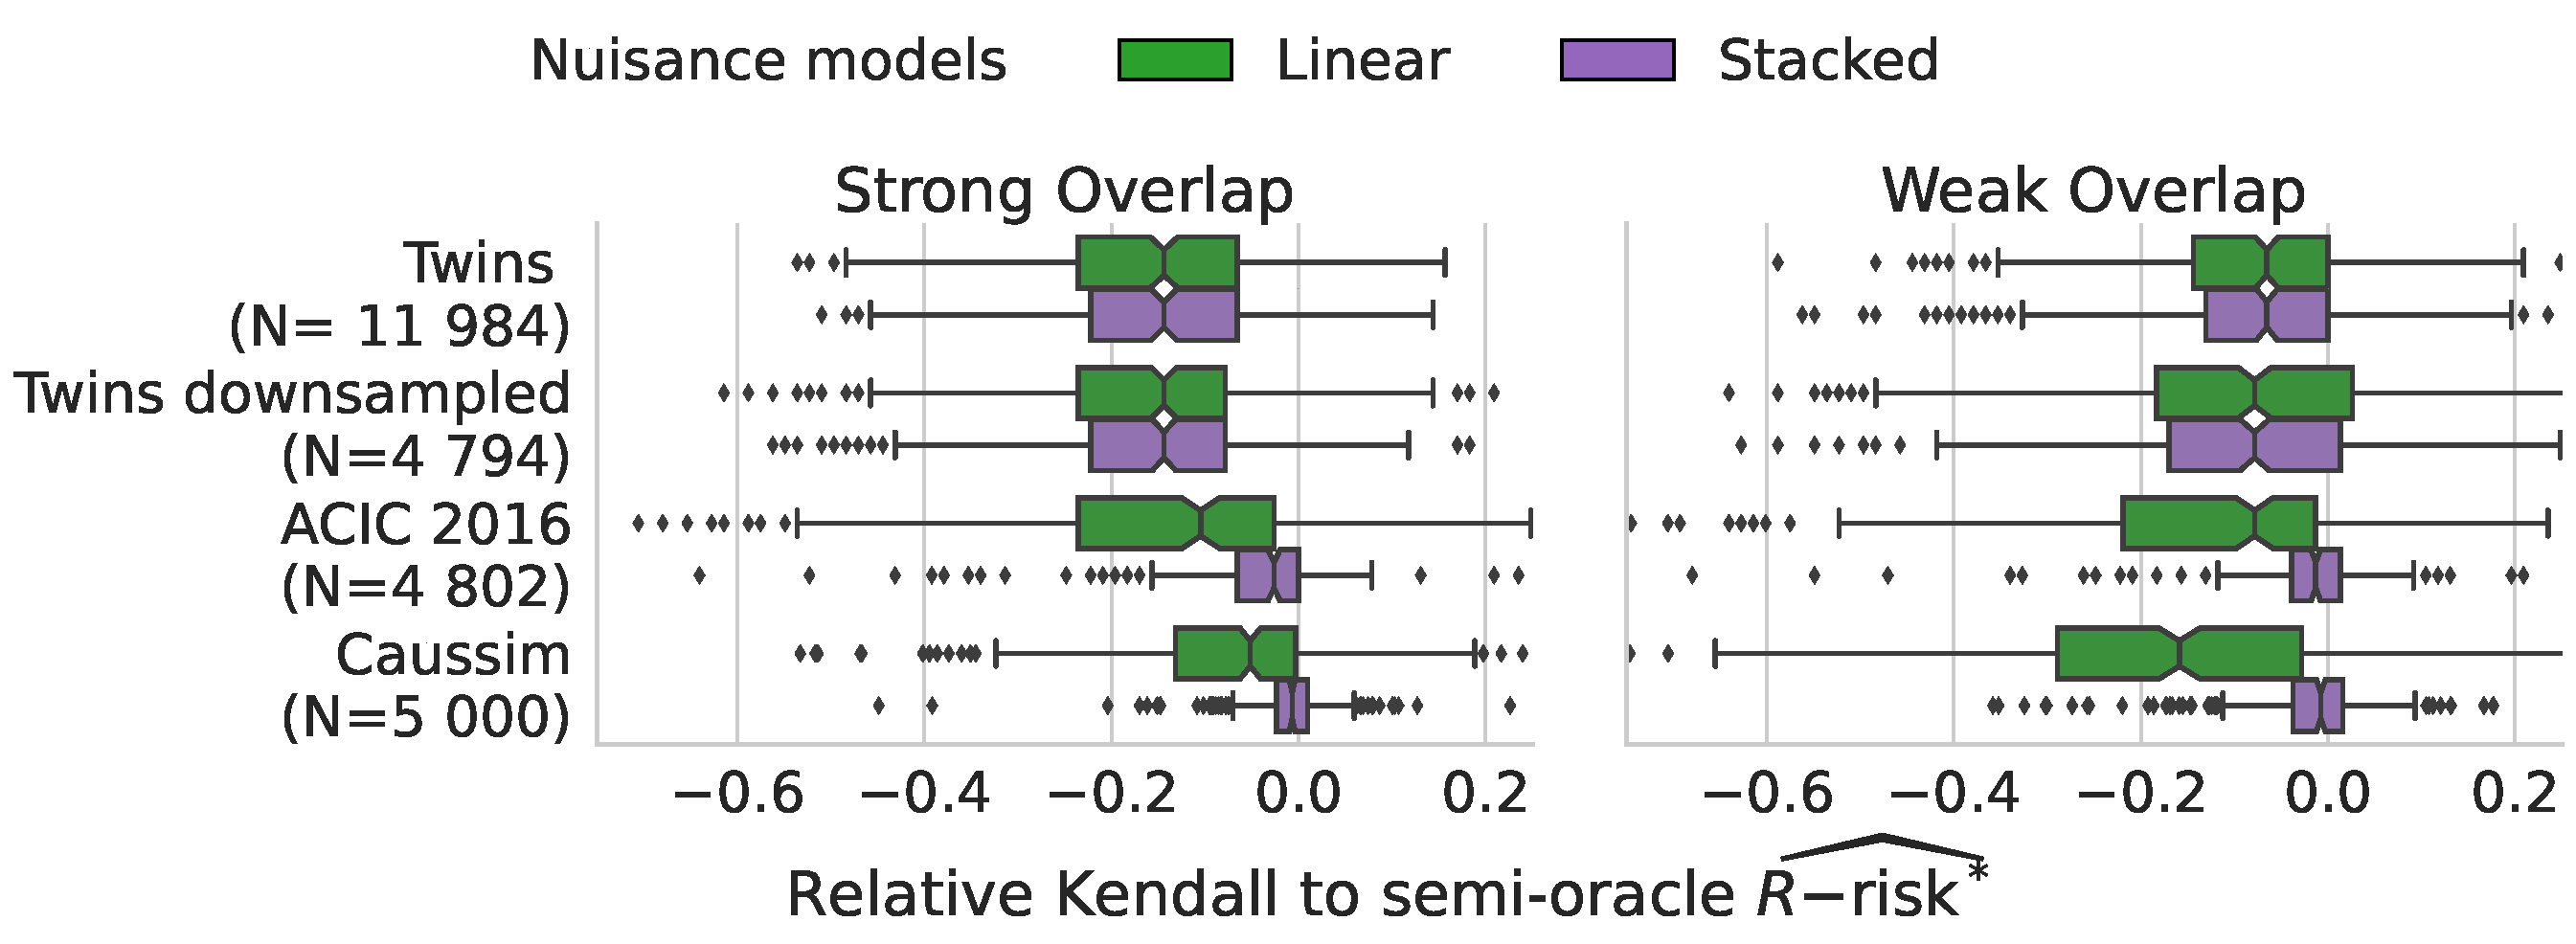
\includegraphics[width=\linewidth]{img/chapter_5/_4_nuisance_models_r_risk_only_3datasets.pdf}
  \caption{\textbf{\textcolor{DarkOrchid}{Stacked
        models} are good overall estimators of the nuisances}:
    Results are shown only for the
    R-risk; Figure \ref{apd:fig:nuisances_comparison}
    details every metrics. For Twins, where the true propensity
    model is linear, \textcolor{DarkOrchid}{stacked} and
    \textcolor{ForestGreen}{linear}
    estimations of the nuisances performs equivalently, even for a downsampled version
    (N=4794). }\label{fig:all_datasets_nuisances_comparison}
\end{figure}

\paragraph{Use 90\% of the data to estimate outcome models, 10\% to
  select them}

The analyst faces a compromise: given a finite
data sample, should she allocate more data to estimate the outcome model,
thus improving the quality of the outcome model but leaving
little data for model selection. Or, she could choose a bigger test set for
model selection and effect estimation. For causal model selection, there
is no established practice (as reviewed in \ref{apd:results:k_fold_choices}).

We investigate such tradeoff varying the ratio between train and test
data size. For this, we first split out 30\% of the data as a holdout set
$\mathcal{V}$ on which we use the oracle response functions to derive
silver-standard estimates of causal quantities. We then
use the standard estimation procedure on the remaining 70\% of the data,
splitting it into train $\mathcal{T}$ and test $\mathcal{S}$ of varying
sizes. We finally measure the error between this estimate and the
silver standard.

We consider two different analytic goals: estimating a average
treatment effect --a single number used for policy making-- and a
CATE --a full model of the treatment effect as a function of covariates
$X$. Given that the latter is a much more complex object than the former,
the optimal train/test ratio might vary. To measure errors, we use for
the ATE the relative absolute ATE bias between the ATE computed with the
selected outcome model on the test set, and the true ATE as evaluated on
the holdout set $\mathcal{V}$. For the CATE, we compare the
$\tau\text{-risk}$
of the best selected model applied on the holdout set $\mathcal{V}$. We explore this trade-off for the ACIC 2016 dataset and the R-risk.

\begin{figure}[!t]
  \begin{minipage}{.5\textwidth}
    \centerline{\textbf{a) CATE estimation error}}
    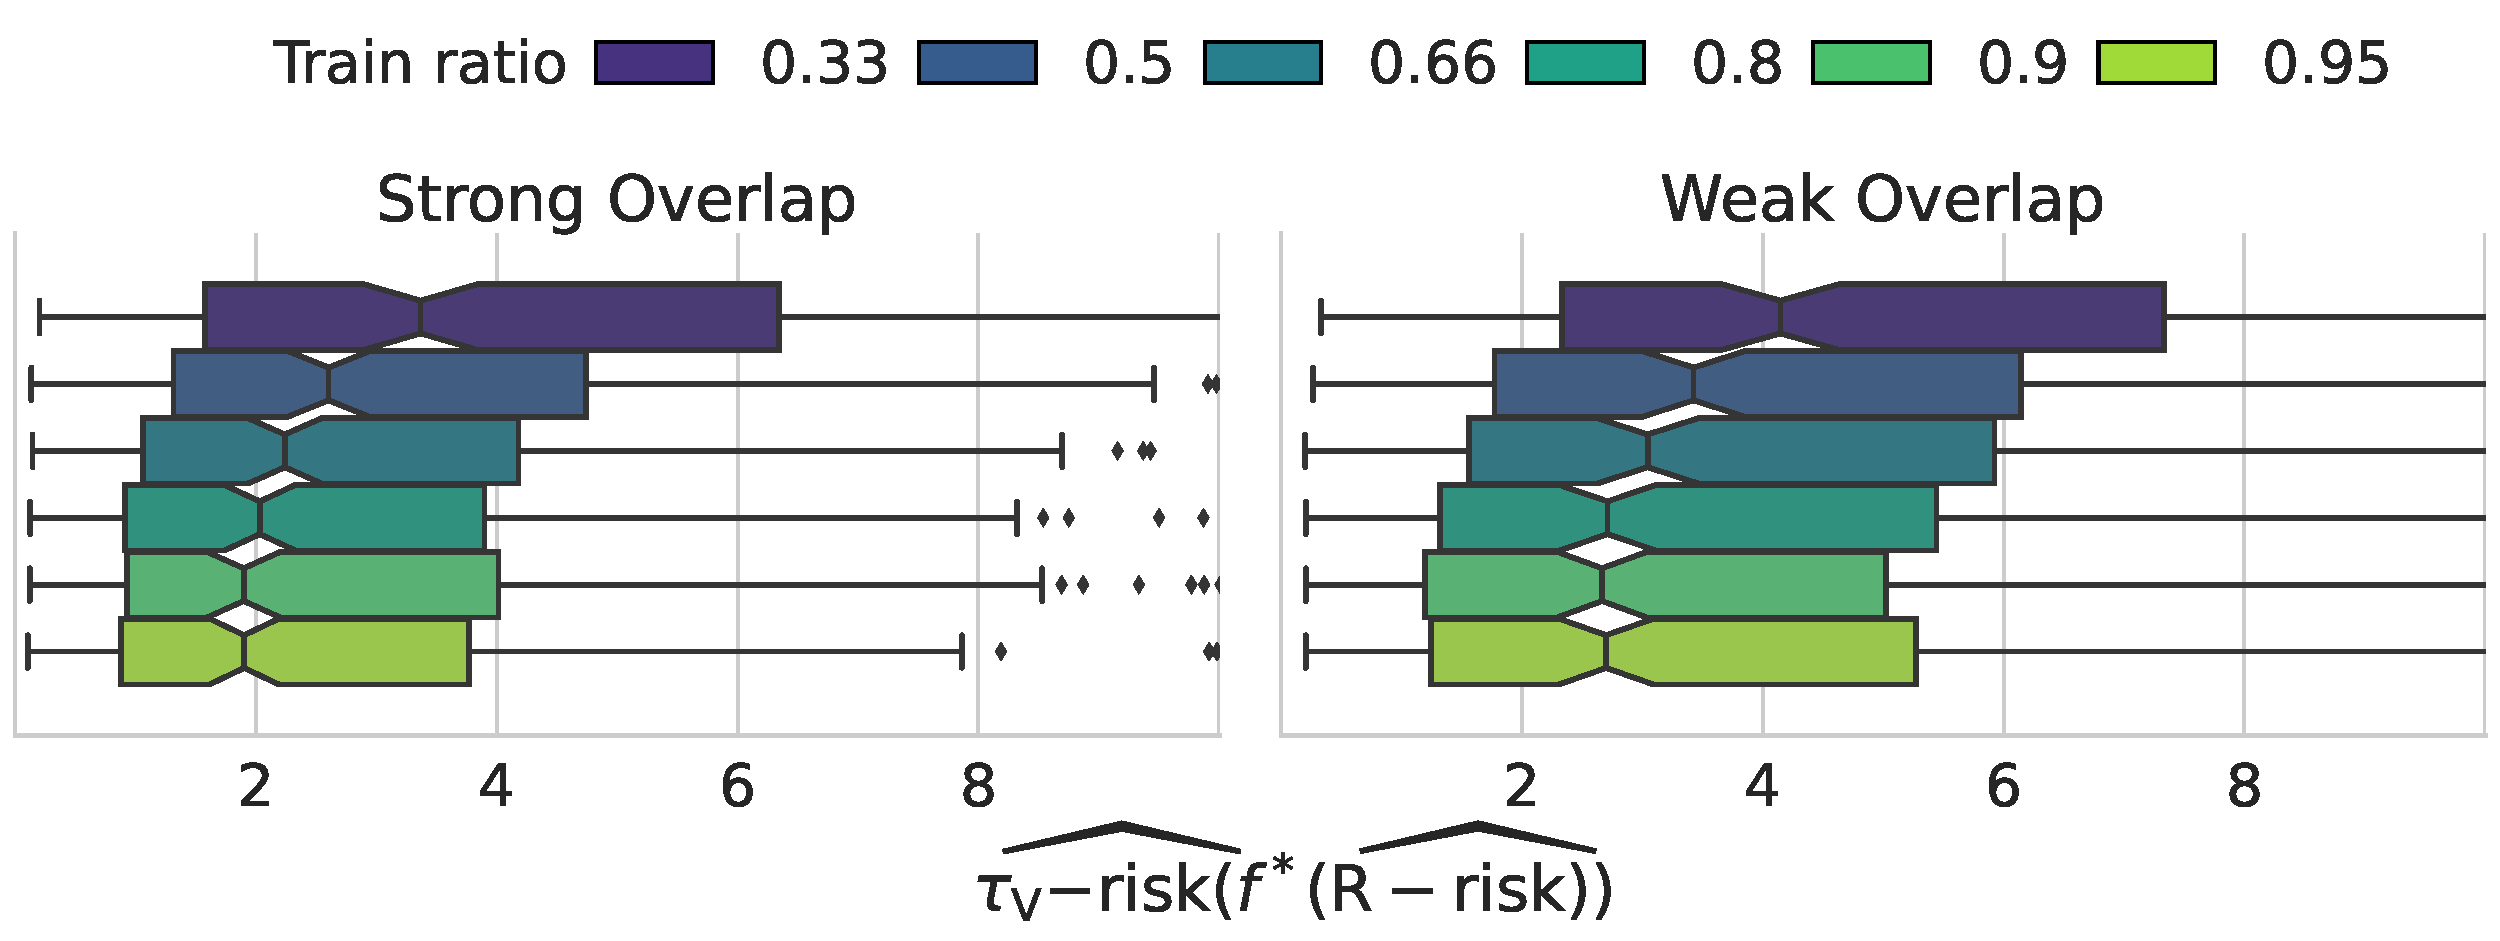
\includegraphics[width=\linewidth]{img/chapter_5/_5_train_size_evaluated_metric_r_risk__evaluation_validation_tau_risk__best_tau_norm__False_norm_False__acic16.pdf}
  \end{minipage}
  %\hspace{0.3\textwidth}
  \begin{minipage}{.5\textwidth}
    \centerline{\textbf{b) ATE estimation error}}
    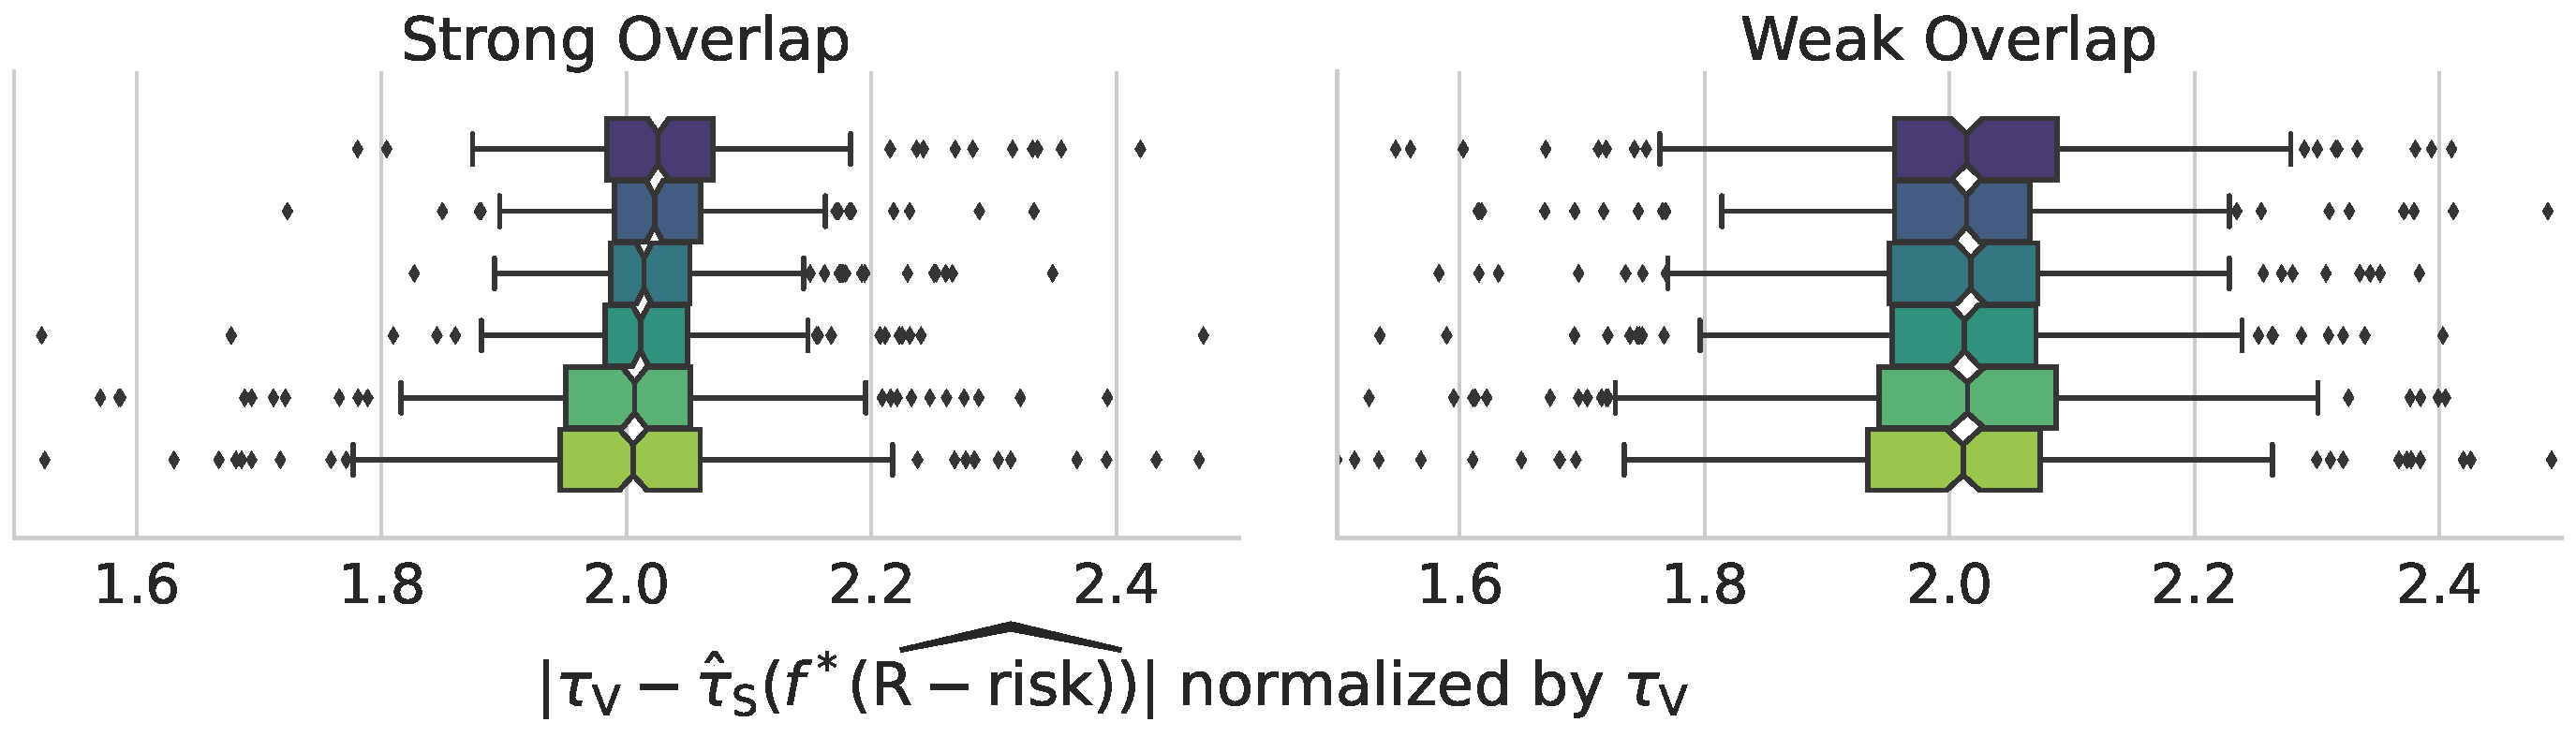
\includegraphics[width=\linewidth]{img/chapter_5/_5_train_size_evaluated_metric_r_risk__evaluation_validation_test_abs_bias_ate__best_tau_norm__False_norm_True__acic16.pdf}
  \end{minipage}%
  \caption{\textbf{a) For CATE, a train/test ratio of 0.9/0.1 appears a good
      trade-off.} b) For ATE, there is a small signal pointing also to
    0.9/0.1 (K=10).
    for ATE. Experiences on 10 replications of all 78 instances of the ACIC 2016
    data.}\label{fig:train_test_ratio}
\end{figure}

Figure \ref{fig:train_test_ratio} shows that a train/test ratio of
0.9/0.1 (K=10) or 0.8/0.2 (K=5) appears best to estimate CATE and
ATE.


\section{Discussion and conclusion}\label{sec:discussion}

Predictive models are increasingly used to reason about causal effects,
for instance in precision medicine to drive individualized decision.
Our results highlight that they should be selected, validated, and tuned
using different procedures and error measures than those classically used
to assess prediction (estimating the so-called $\mu\text{-risk}$).
Rather, selecting the best outcome model according to the $R\text{-risk}$
(eq.\,\ref{def:r_risk}) leads to more valid causal estimates.

\paragraph{Nuisance models: more gain than pain}
%
Estimating the $R\text{-risk}$ requires a more complex procedure than
standard cross-validation used \emph{e.g.}~in machine learning: it involves
fitting nuisance models necessary for model evaluation, though our
results show that these can be learned on the same set of data
as the outcome model evaluated.

The nuisance models must be well estimated (Figure
\ref{fig:all_datasets_nuisances_comparison}). However these models are
easier to select and control than a causally-valid outcome model,
as they are associated to errors on
observed distributions. Our results show that using for nuisance models
a flexible stacking-based family of estimator suffices for good model selection.
%
In fact, a feasible $R\text{-risk}$ --where the nuisances
are estimated-- performs almost as well as an oracle $R\text{-risk}$ --where the
nuisances are known. This may be explained by
results that suggest that estimation errors on both
nuisances partly compensate out in the
$R\text{-risk}$ \citep{daniel2018double,kennedy2020optimal,nie_quasioracle_2017,chernozhukov_double_2018,zivich2021machine,naimi2021challenges}.

Note that propensity score models must be selected to estimate
the individual posterior probability. For this, we used the Brier score,
which is minimized by the true individual probability. An easy mistake is to
use calibration errors popular in machine learning
\citep{platt_probabilistic_1999,zadrozny_obtaining_2001,niculescu-mizil_predicting_2005,minderer_revisiting_2021}
as these select not for the individual posterior probability but for an
aggregate error rate \citep{perez2022beyond}.


\paragraph{Extension to binary outcomes}
While we focused on continuous outcomes, in medicine, the target outcome is
often a categorical variable such as mortality status or diagnosis. In this
case, it may be interesting to focus on other estimands than the Average
Treatment Effect $\mathbb{E}[Y(1)] -\mathbb{E}[Y(0)] $, for instance the
relative risk $\frac{\mathbb P(Y(1) = 1)}{\mathbb P(Y(0) = 1)}$ or the odd
ratio, $\frac{\mathbb P(Y(1) = 1) / [1 - \mathbb P(Y(1) =1)]}{\mathbb P(Y(0) =
  1) / [1 - \mathbb P(Y(0) = 1]}$ are often used \citep{austin2017estimating}.
While the odds ratio is natural for case-control studies \citep{rothman2008case},
other measures can reduce heterogeneity \citep{colnet2023risk}. In the log
domain, the ratios are written as a difference, the framework studied here
(\autoref{sec:causal_model_selection:setting}) can directly apply. In
particular, the log odds ratio is estimated by the common cross-entropy loss (or
log loss) as in logistic regression.

\paragraph{More $R\text{-risk}$ to select models driving decisions}

Prediction models have flourished because their predictions can be easily
demonstrated and validated on left-out data. But they require more
careful validation for decision making, using a metric accounting for the
putative intervention, the $R\text{-risk}$. Even when treated and
untreated population differ little, as in RCTs, the $R\text{-risk}$
brings a sizeable benefit. To facilitate better model selection, we provide Python
code \footnote{\url{https://github.com/soda-inria/causal_model_selection}}.
Using the $R\text{-risk}$ does make evaluation more
complicated not only because the procedure is more involved, but also
because each intervention requires a dedicated evaluation. However, such
off-policy evaluation remains much less costly than the recommended good
practice of impact evaluation testing the ability of a prediction model
to actually guide patient health \citep{hendriksen2013diagnostic}. Also,
the model-selection procedure puts no constraints on the models used to
build predictive models: it opens the door to evaluating a wide range of
models, from gradient boosting to convolutional neutral, or language
models.

%Nevertheless, from a practical perspective, our study establishes that
%the $R\text{-risk}$ is the best option to select predictive models for
%causal inference, without requiring assumptions on the data-generating
%mechanism, the amount of data at hand, or the specific estimators .


% XXX: need a final positive
% Maybe that as our work has no
% requirement on the learning procedure,
% it contributes to ensuring the
% validity of causal inference on complex databases such as clinical
% records with a lot of open-ended text that must be analyzed with
% language models.




\chapter{Conclusion}\label{chapter:conclusion}

\minitoc

%Healthcare burden in modern world is access to healthcare, and chronic disease
%ie. resource issues more than better products, our methodological toolbox to
%distinguish between good and bad management is not adapted to the task since it
%involved complicated process specific to each situation. Some can be borrowed
%from economics, but specificities from epidemiology should be mixed in. 
Modern healthcare burdens and costs are driven by chronic diseases where death
is not the only outcome of interest. Focus on smaller rewards, on which
experiments are easier to conduct and where error is possible: it would allow
better learning for decision making since we can repeat more experiments (limit:
signals could be highly delayed).

Modern collection of data in healthcare makes it a domain closer to social
sciences than usually considered. It involves institutions and individuals with
complex data collection patterns and choices that are seldom well controlled by
the researcher alone. Therefore, we should bridge traditional
statistics with econometrics and social sciences to analyze it. This does not
impose to abandon the scientific method, but to adapt it to constant
distribution shifts and unkown complex mechanisms.

% Pattern exists in the massive data collected: we need to extract them
% automatically and articulate these with scientific questions guided by
% knowledge domain.
Complex patterns in big data call for machine learning methods, which haveq been shown to
highly perform . Text is pervasive, we are using it to communicate and to log
most of our information. We can rely pretraining models outside the healthcare
domain. We should leverage it more in the context of care (limit: temporality is
hard to capture but is a key aspect of causal inference).

% Those problem are more pragmatic than theoretical. Thus, data and conclusions need to circulate. 
The unreasonable effectiveness of healthcare data is yet out of reach due to
hugely difficult transfer of models or administrative barriers to access data
(due to multiplicity of the involved actors). This forces us to rely on
efficient techniques that make the best of medium-sized data or rely on sharable
sources of knowledge (aggregated statistics, federated learning approaches,
ontologies, ...).

Ultimately, I am convinced that resource constraints and the ever-increasing
demand on healthcare links care effectiveness to equity. Some patients will
always be less treated than others: public health should seek for random
repartition of these mistreated patients conditionally on patient conditions.

\clearpage
\begin{appendices}
  \renewcommand{\thechapter}{\Alph{chapter}} % Redefine chapter numbering to letters
  \renewcommand{\thesection}{\thechapter.\arabic{section}} % Include chapter letter in section numbering
  \renewcommand{\thesubsection}{\thesection.\arabic{subsection}} % Include chapter letter in subsection numbering

  \chapter{Chapter \ref{chapter:intro}}\label{apd:intro}

  \section{Statistical learning theory}\label{apd:intro:statistical_learning}

  I recall here the formal definition of the regression problem in statistical
  learning and I refer to \cite{hastie2009elements} for the classification
  problem.

  Given n pairs of (features,
  outcome) noted $(x, y) \in \mathcal X \times \mathcal{Y}$ identically and
  independently distributed (i.i.d) , the goal is to find a function $f:
    \mathcal{X} \rightarrow \mathcal{Y}$ that approximates the true value of $y$
  ie. $f(x) \approx y$. One need to define a loss function $\ell$ that define
  proximity between the predicted value $\hat{y} = f(x)$ and the true value
  $y$. Usually, for continuous outcomes, the squared loss is used. Finally,
  when choosing among a family of functions $f \in \mathcal{F}$, the best possible function $f^{\star}$
  minimizes the expected loss $\mathcal{E}(f^{\star})$:

  \begin{equation}
    f^{\star} = \argmin_{f \in \mathcal{F}} \mathbb{E} \big [ (\hat{y} - y)^2 \big]
  \end{equation}

  In finite sample regimes, the expectation is not accessible since we only have
  access to a finite number of data pairs ${(x_i, y_i)}_{i=1..n}$. So in
  practice, we aim to minimize the empirical loss $\mathcal{E}(f^{\star})$::
  \begin{equation}
    \hat f = \argmin_{f \in \mathcal{F}} \sum_{i=1}^{n} \big [ (\hat{y}_{i} - y_{i})^2 \big]
  \end{equation}

  In most interesting problems, there is some randomness involved in the $(x,y)$
  association, either due to inherent randomness or to the lack of important
  information in $x$. This is modeled by assuming it independent of the features
  and with mean zero: $y = g(x) + e$, with $\mathbb E[e]=0$. The best possible estimator
  is thus $g$, yielding the Bayes error \highlight{bayes_error}{\color{black} $\mathcal{E}(g) =
      \mathbb{E} \big [ (g(x) + e - g(x))^2 \big]=\mathbb{E}[e^2]$}. This error
  cannot be avoided.

  Finally, the generalization error of the estimator $\hat f$ can be decomposed as:
  \begin{equation}
    \mathcal{E}(\hat f) = \highlight{bayes_error}{\color{black} $\mathcal{E}(g)$} +
    \highlight{approximation_error}{$(\mathcal{E}(f^{\star}) - \mathcal{E}(g))$} +
    \highlight{estimation_error}{$(\mathcal{E}(\hat{f}) - \mathcal{E}(f^{\star}))$}
  \end{equation}


  The \highlight{approximation_error}{second term} is the approximation error: the difference between the best
  estimator in the family of estimator considered and the Bayes estimator. It
  decreases for larger $\mathcal{F}$.

  The \highlight{estimation_error}{third term} is the estimation error related to the
  sampling noise of the data. It decreases with raising n --if we have a lot of
  data points. It increases for larger $\mathcal{F}$. This decomposition
  highlights the choice of a practitioner for applying regression: she must
  choose a function class $\mathcal{F}$ flexible enough to avoid underfitting
  the data but restrictive enough to avoid a high estimation error.

  \section{Statistical models}\label{apd:intro:statistical_models}

  We recall briefly how trees, random forests and boosting work. For more
  details, see \citep{hastie2009elements}.

  \subsection{Trees}\label{apd:intro:trees}

  Decision trees are a class of models that recursively split the feature space
  into a set of rectangles --called nodes, and assign a constant value to each
  rectangle. They can be use both for classification or regression. If used for
  regression, a new split from one region into two subregions is chosen as
  follows. Among all variable and split possibility, choose the split that
  minimizes the error --typically the squared error-- between the average of the
  outcomes over the two newly regions and the individual outcomes. If used for
  classification, splits are chosen by minimizing some impurity measure of the
  class probabilities over the two new created nodes instead of the squared
  error. A typical impurity measure is the Gini index $\sum_{k=1}^K \hat p_{mk}
    (1-\hat p_{mk})$ where $\hat p_{mk}$ is the empirical probability of class k
  in node m. The complexity of a tree is determined by its maximal depth --ie,
  the maximum number of splits before reaching a terminal node --called a leaf.

  Figure \ref{fig:tree_regression} illustrates on a toy example two regression
  trees of depth 2 and 5.

  \begin{figure}
    \centering
    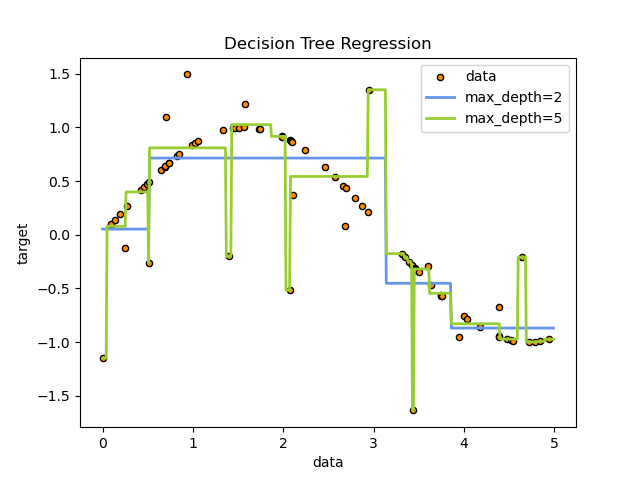
\includegraphics{img/chapter_1/sphx_glr_plot_tree_regression_001.png}
    \caption{Illustration of two regression tress of depth 2 and 5.\\Original
      figure from \url{https://scikit-learn.org/stable/modules/tree.html}.}%
    \label{fig:tree_regression}
  \end{figure}

  Trees have the advantages to have small biases and to be grown rapidly from
  both categorical or continuous variables. However, they suffer from
  instability and thus have high variance: Small changes in the data can yield
  to very different series of split.

  \subsection{Random Forests}\label{apd:intro:random_forests}

  Random forests \citep{breiman2001random} have been proposed to overcome the
  instability of trees. A random forest averages the results of B trees grown
  identically, thus not affecting the bias of the whole estimator. The variance
  reduction is performed by forcing the trees to be different from each other.
  This is achieved by introducing randomness in the tree growing procedure. At
  each split, only a random subset of features are selected. On average, the
  errors of each individual tree cancel each other, thus reducing the high
  variance of each individual tree without a high increase in bias.

  \subsection{Gradient Boosting}\label{apd:intro:boosting}

  Gradient boosting \citep{friedman2001greedy} is a method that iteratively sums
  weak learners --typically trees-- to each other. Each new weak learner
  improves over the errors of the previous averaged estimators. The final
  estimator has the same form than a random forest, but require substantially
  less trees.


  %\section{Causal Diagrams}\label{apd:causal_diagrams}
  \chapter{Chapter \ref{chapter:cdw}}\label{apd:cdw}

  %\renewcommand{\thesubsection}{\thesection.\alph{subsection}}
  % Include only the SI item label in the paragraph heading. Use the
  % \nameref{label} command to cite SI items in the text.
  \section{List of interviewed stakeholders with their
    teams}\label{apd:cdw:table:expert_teams}

  \begin{table}[!ht]
    \centering
    \begin{tabular}{ll}
      \thickhline
      Clinical Data Warehouse & Teams                                             \\
      \thickhline
      CDW\_AMIENS             & IT : 1,MID : 1                                    \\
      CDW\_ANGERS             & Data Direction : 1                                \\
      CDW\_APHM               & Clinician : 1,CDW team : 2                        \\
      CDW\_APHP               & CDW team : 4,IT : 5                               \\
      CDW\_BORDEAUX           & CDW team : 1,Inserm : 1,public health : 2         \\
      CDW\_BREST              & CDW team : 1,MID : 1                              \\
      CDW\_DIJON              & CDW team : 1                                      \\
      CDW\_EDSAN              & CDW team : 2,MID : 1                              \\
      CDW\_HCL                & Clinician : 1,Data Direction : 1,IT : 1,Inserm    \\
      CDW\_INCLUDE\_LILLE     & Administration : 2,CDW team : 3,public health : 2 \\
      CDW\_MARTINIQUE         & CDW team : 1,public health : 1                    \\
      CDW\_MONTPELLIER        & Data Direction : 2,MID : 1,public health : 1      \\
      CDW\_NANCY              & CDW team : 2,public health : 2                    \\
      CDW\_NANTES             & CDW team : 2,public health : 1                    \\
      CDW\_POITIERS           & IT : 2,CRD : 1                                    \\
      CDW\_PREDIMED\_CHUGA    & CDW team : 3,public health : 2                    \\
      CDW\_REIMS              & Clinician : 1,CDW team : 1                        \\
      CDW\_RENNES             & CDW team : 2,public health : 2                    \\
      CDW\_STRASBOURG         & CDW team : 2,public health : 2                    \\
      CDW\_TOULOUSE           & CDW team : 1                                      \\
      CDW\_TOURS              & CDW team : 1                                      \\
      \thickhline
    \end{tabular}
  \end{table}

  \clearpage


  \begin{landscape}
    \section{Interview form} \label{apd:cdw:interview_form}
    \begin{table}[h!]
      \centering
      \resizebox{1.4\textwidth}{!}{%
        \begin{tabular}{|l|l|}
          \hline
          \textbf{Topics}                                                        &
          \textbf{Questions}
          \\ \hline
          \multirow{5}{*}{\begin{tabular}[c]{@{}l@{}}Initiation and Construction
                              of \\ the Clinical Data Warehouse\end{tabular}} &
          How was the initiative born, when, which team(s) involved in the
          construction? A Data warehouse to meet what initial needs ?                                                                 \\
          \cline{2-2}                                                            & What was (is) the articulation between the medical
          informatics / engineer(s) / Clinical Research Department  and user
          team(s), biostatistics ?                                                                                                    \\ \cline{2-2} & Governance: How
          should the teams be organized for the creation and maintenance of the
          warehouse, data access, and project teams?                                                                                  \\ \cline{2-2} &
          \begin{tabular}[c]{@{}l@{}}What types of data are present in the
            warehouse
            from the
            following
            non-exhaustive
            list: \\
            Billing
            codes ,
            other
            administrative
            data,
            other
            procedures,
            structured
            procedures
            and
            diagnoses,
            structured
            biology
            measures,
            \\
            structured
            drug
            treatments,
            emergencies,
            resuscitation,
            anesthesia,
            texts
            (letters,
            Clinician
            Reports),
            imaging,
            anatomopathology,
            sequencing.\end{tabular}
          \\
          \cline{2-2}
                                                                                 & What
          are the
          medico-social/social
          data,
          especially
          from
          social
          and
          medico-social
          institutions
          ?
          \\
          \hline
          \multirow{6}{*}{Current status - Ongoing and finished projects}        &
          \begin{tabular}[c]{@{}l@{}}Who are the main users? For what purposes
            (research,
            quality
            improvement,
            management,
            clinical
            usage)?
            \\ Which
            therapeutic
            area(s)?\end{tabular}
          \\
          \cline{2-2}
                                                                                 &
          \begin{tabular}[c]{@{}l@{}}What are the major types of projects from the
            following
            non-exhaustive
            list: \\
            Cohort
            development,
            descriptive
            epidemiology,
            analytical
            (comparative)
            epidemiology
            with/without
            randomization,
            monitoring
            and
            dashboards,
            \\indicators,
            inclusion
            in
            clinical
            trials.\end{tabular}
          \\
          \cline{2-2}
                                                                                 & How
          many
          projects
          are
          completed
          /
          started
          /
          planned?
          \\
          \cline{2-2}
                                                                                 & What
          are the
          tools
          and
          methods
          used for
          these
          projects?
          Cohort
          building
          tool,
          standard
          data
          formats,
          NLPs,
          ...
          \\
          \cline{2-2}
                                                                                 & Is
          there a
          valorization
          strategy
          for the
          Clinical
          Data
          Warehouse?
          \\
          \cline{2-2}
                                                                                 & What
          connections
          with
          external
          sources
          such as
          the
          national
          health
          data
          platform,
          the
          outpatient
          data,
          the
          general
          practitioner
          data,
          the
          research
          cohorts
          ?                                                                                                                           \\
          \hline
          \multirow{3}{*}{Opportunity and obstacles}                             & What
          are the main difficulties encountered during data warehouse projects?
          \\ \cline{2-2} & Are there themes that deserve more encouragement from
          the HAS?
          \\ \cline{2-2} & What skills are needed? Are there any skills or
          technical resources missing?
          \\ \hline
          \multirow{11}{*}{\begin{tabular}[c]{@{}l@{}}Quality criteria for
                               observational research\end{tabular}}       & Coverage: How
          is it monitored? Geographically/by department? Time-wise? By what means?
          \\ \cline{2-2} & Cleaning: How are patient duplicates and source
          alignment managed?
          \\ \cline{2-2} &
          \begin{tabular}[c]{@{}l@{}}Database Network: Does the warehouse belong
            to a
            health
            database
            network?\end{tabular}
          \\
          \cline{2-2}
                                                                                 &
          \begin{tabular}[c]{@{}l@{}}Data quality: Are there automatic reports on
            data
            quality?
            Frequency,
            design,
            code and
            documentation
            available?
            Presence
            of
            dedicated
            personnel
            \\ or
            even a
            team to
            check
            the
            quality
            of the
            data
            continuously,
            and to
            carry
            out
            quality
            controls
            of the
            data on
            the
            central
            base, on
            the
            study
            bases?\end{tabular}
          \\
          \cline{2-2}
                                                                                 &
          \begin{tabular}[c]{@{}l@{}}Data life cycle: Is there a reference
            document
            on the
            different
            stages
            of the
            data
            life
            cycle?
            \\ How
            is this
            document
            kept up
            to date
            with the
            constant
            evolution
            of the
            warehouse?
            In what
            form? \\
            How is
            this
            documentation
            managed,
            accessed,
            updated
            and
            corrected?
            Precise
            description
            of the
            integrated
            fields?\end{tabular}
          \\
          \cline{2-2}
                                                                                 &
          \begin{tabular}[c]{@{}l@{}}Harmonization procedure: What are the data
            structures/formats
            and
            coding
            systems
            used? \\
            (eHop,
            I2B2,
            OMOP,
            HL7
            FHIR,
            other
            ?)\end{tabular}
          \\
          \cline{2-2}
                                                                                 &
          \begin{tabular}[c]{@{}l@{}}Machine learning: If machine learning systems
            are used
            (e.g.
            for
            extracting
            and
            structuring
            information),
            is there
            specific
            documentation
            on their
            performance?
            \\ For
            manual
            coding
            (e.g.
            labelling),
            is there
            a coding
            guide?
            Has a
            measurement
            of
            inter-coder
            consistency
            been
            conducted?\end{tabular}
          \\
          \cline{2-2}
                                                                                 &
          De-identification:
          Elements
          on
          de-identification
          if
          applicable,
          performance
          metrics
          \\
          \cline{2-2}
                                                                                 &
          \begin{tabular}[c]{@{}l@{}}Constructed phenotypes: Are there operational
            definitions
            of
            target
            populations
            (study
            cohorts)
            and how
            are
            these
            compared
            to
            conceptual
            definitions,
            i.e., \\
            business
            and
            scientific
            definitions?
            Is there
            a study
            of
            FPR/TPR
            in
            relation
            to a
            reference
            standard?
            Are
            these
            definitions
            made
            public
            either
            with the
            study \\
            results
            or in
            the
            documentation
            of the
            warehouse?\end{tabular}
          \\
          \cline{2-2}
                                                                                 &
          \begin{tabular}[c]{@{}l@{}}Transparency: Are the studies registered on a
            dedicated
            or
            pre-existing
            portal
            (epidemio-France,
            encepp
            (EU),
            clinicaltrials.gov
            (US))?
            \\ Are
            the
            study
            codes
            made
            accessible
            as for
            opensafely?
            Are the
            publications
            accessible
            in open
            access,
            once the
            studies
            are
            completed?\end{tabular}
          \\
          \cline{2-2}
                                                                                 &
          \begin{tabular}[c]{@{}l@{}}Multidisciplinarity: Are the project teams
            multidisciplinary? Specification of the participations for each part of
            the analysis from the data collection \\ from the raw Information
            System.\end{tabular}
          \\ \hline
          \multirow{2}{*}{Topics of interest to the HAS}                         &
          \begin{tabular}[c]{@{}l@{}}Quality Department: quality indicators
            (french
            IQSS):
            coordination
            (patient
            assessment
            for
            discharge,
            patient
            contact
            at D+1),
            quality
            of the
            liaison
            letter),
            \\
            management
            (eligibility
            for the
            outpatient
            surgeries,
            pain
            management)\end{tabular}
          \\
          \cline{2-2}
                                                                                 &
          \begin{tabular}[c]{@{}l@{}}Health Technology Assessment Department:
            hospital biology activity (description), adverse events associated with
            procedures, post-registration studies \\(procedures, early access
            oncology). Evaluation of procedures: e.g. biological and imaging
            procedures performed in hospitals, genetic tests in oncology and rare
            diseases.\end{tabular}
          \\ \hline
          open discussion                                                        &                                                    \\
          \hline
        \end{tabular}%
      }
      %\caption*{Interview form.}

    \end{table}
  \end{landscape}

  \section{Study data tables}\label{apd:cdw:study_tables}

  The data tables used to produce the figures in the results section are available
  at the following url:

  \url{https://gitlab.has-sante.fr/has-sante/public/rapport_edsh/}.

  \begin{itemize}
    \item The guests table concerns the individuals interviewed, the interview dates, the
          positions and the membership of a specific team: \url{https://gitlab.has-sante.fr/has-sante/public/rapport_edsh/-/blob/master/data/cycle_eds/cycle_eds_intervenants.csv}
    \item  The warehouse table collects information about the CDW: \url{https://gitlab.has-sante.fr/has-sante/public/rapport_edsh/-/blob/master/data/cycle_eds/cycle_eds_entrepots.csv}
    \item The study table references the in-progress study titles and objectives from 10 public declarative portals in progress: \url{https://gitlab.has-sante.fr/has-sante/public/rapport_edsh/-/blob/master/data/cycle_eds/cycle_eds_etudes.csv}
  \end{itemize}




  \chapter{Chapter \ref{chapter:predictive_models}}\label{apd:predictive_models}

  \section{Code}

  The code for the experiments is available at
  \url{https://gitlab.inria.fr/soda/medical_embeddings_transfer}.\md{need to move
    the package to github.}

  A fork of the CEHR-BERT implementation is available at \url{https://github.com/strayMat/cehr-bert}. It was necessary
  to adapt the code to our data format and to the AP-HP computing environment.

  All count encoding and static embedding featurizers are available as a standalone
  package at \url{https://gitlab.com/strayMat/event2vec}.


  \section{Predictive models and tasks on EHRs}\label{apd:review_predictions}

  \subsection{Why predictive models in healthcare ?}\label{apd:review_tasks}%


  \paragraph{Risk stratification in the clinic}

  % risk stratification
  Early prediction of a complication calls for early intervention. Focused on short
  term interventions in the clinic, these models seek to increase short or long
  terms outcomes of the patients thanks to early intervention before deterioration
  \citep{tang2007global, rothman2013development, wong2021external}. Those so-called alert systems
  \citep{yu2018artificial} map complex inputs --eg. a combination of nursing
  assessments, vital signs, laboratory results and cardiac rhythms-- to simpler
  risk scores, allowing clinicians to rapidly judge the evolution of the patient.
  % Long term prevention
  The same kind of risk stratification is also used for long term prevention under
  the term \emph{screening}.
  %

  \paragraph{Predict to identify important risk factors}

  Risk stratification is close to the research of risk factors.
  % historical model: risk factor
  The Framingham risk score, one of the earliest predictive models in medicine was
  designed to predict Coronary heart disease risk by fitting a cox model using
  seven features on 5300 patients: age, cholesterol, systolic blood pressure,
  hematocrit, ECG status, smoking at intake, and relative body weight
  \citep{brand1976multivariate}. The authors aim to identify important risk factors
  allowing the selection of individuals for intervention programs.
  % biostatistics view
  Biostatistics also focuses on risk factors for subgroup identification, framing
  this task as therapeutics \citep{steyerberg2009applications} or heterogeneous
  treatment effect \citep{harrell2001regression}.
  %

  \paragraph{Prognosis for automated decision-making}
  % Roots in Artificial Intelligence in Medicine
  Multiple applications of Artificial Intelligence in Medicine were already
  discussed in the early 80s \citep[Chapter~1]{Szolovits1982artificial}:
  diagnostic and therapeutic program for glaucoma (CASNET), diagnostic and therapy
  for infectious diseases (MYCIN) \citep{shortliffe1976computer}, therapic advice
  for patients with heart disease, diagnosis in general internal medicine
  (INTERNIST-I). In this line of work, a good predictive model often serves as a
  module in a larger decision-making system aiming at personalized medicine
  \citep{topol2019high}.

  \paragraph{Predict to better plan and pilot}

  In complex healthcare organizations, accurate individual predictions help to
  use efficiently constrained medical resources \citep{topol2019high}. One of such
  operational tasks is Length Of Stay (LOS) prediction, allowing to plan the
  number of beds and members of staff required, identify individual outliers
  \citep{verburg2017models}. %
  Identified as a quality of care indicator, unplanned readmission at 30 days is
  used to benchmark and finance hospitals in several countries
  \citep{cms2019readmission, kristensen2015roadmap}. In addition to the risk
  reduction for patients, it incentivized the hospital to develop better
  prediction models for unplanned readmission.
  % A plethora of such models have been published: \citep{zhou2016utility}, structured data (prescriptions,
  % diagnoses, procedures, demographic data) combined with logistic
  % regression, random forests, boosting and neural networks
  % yielding up to 0.69 ROC AUC \citep{dhalluin2020comparison}, Bert on clinical notes
  % yielding 0.80 ROC AUC \citep{jiang2023health}.

  Interestingly, recent developments of predictive models on EHRs (described in next section) focused mainly on administrative tasks and
  less on the risk factors or the intervention aspect.

  \subsection{Predictive models on EHRs: from simple to complex}%
  \label{apd:review_models}%

  \paragraph{Predictions on EHRs originally used linear models on few carefully selected statics variables}
  Early work for predictive models on EHR used \textcolor{M}{parsimonious logistic regression}
  (selecting 10 variables on average) to predict \textcolor{O}{Heart Failure} (12\% case
  prevalence) within 6 months reaching \textcolor{S}{0.77 AUC} \citep{wu2010prediction}.

  \cite{goldstein2017opportunities} identified key characteristics of 107 studies
  on predictive models on EHRs: a very large study size (median=26,100), few
  predictors are included (median = 27 variables), few longitudinal data (37
  studies), half multi-center studies. The tasks and performances were
  \textcolor{O}{mortality} with \textcolor{S}{0.84 AUC}, \textcolor{O}{clinical
    prediction (various clinical endpoints)} with \textcolor{S}{0.83 AUC},
  \textcolor{O}{hospitalization} with \textcolor{S}{0.71 AUC},
  \textcolor{O}{service utilization} with \textcolor{S}{0.71 AUC}.
  \textcolor{M}{Generalized linear models such as logistic regression or Cox
    regression} (87 studies) were the most common, followed by \textcolor{M}{Bayes
    methods} (11 studies), \textcolor{M}{random forests} (10 studies) and
  \textcolor{M}{regularized regressions} (7 studies).

  \paragraph{Including high-cardinality and time-varying features thanks to neural networks}

  Acknowledging the high cardinality of medical vocabularies used in EHRs, medical
  informatics leveraged representation learning (mostly algorithms used in Natural
  Language Processing) to embed them into low dimensional feature spaces
  \citep{shickel2017deep}. The goal was to reduce the costly feature engineering
  work used by traditional predictive models.

  This line of work focused first on concept representations:
  \textcolor{M}{restricted bolzmann machines} for \textcolor{O}{suicide
    predictions} (13.1\% prevalence) \citep{tran2015learning}.

  Then it included time: word2vec with temporal contexts
  \citep{beam2019clinical}, \textcolor{M}{convolutional neural networks} for
  \textcolor{O}{unplanned readmission} at 6 months (balanced case/control) with
  \textcolor{S}{0.82 AUC} \citep{nguyen2016mathtt}, \textcolor{M}{LSTM} for
  \textcolor{O}{diagnosis} from physiological signals with \textcolor{S}{0.86
    weighted ROC AUC and 0.12 precision at 10} \citep{lipton2016learning},
  \textcolor{M}{recurrent neural networks} for \textcolor{O}{heart failure}
  (selected 9 to 10 control to cases) with \textcolor{S}{0.88 AUC}
  \citep{choi2017using}, \textcolor{M}{recurrent neural networks} for
  \textcolor{O}{Length Of Stay over 7 days} (20.68\% prevalence),
  \textcolor{O}{mortality} (1.74\% prevalence) and \textcolor{O}{30-day
    readmission} (12.93\% prevalence) with respectively \textcolor{S}{0.79, 0.87 and
    0.70 AUC} all using 24 first hours of observation data
  \citep{beaulieu2021machine}.


  Rare benchmarks of these different methods include :
  \begin{itemize}
    \item \cite{harutyunyan2019multitask} benchmarked four clinical tasks on
          MIMIC-III database, a EHR rich in signals since it covers Intense Care
          Units. The tasks were in-hospitality prediction based on the first 48
          hours of data, decompensation prediction at each hour, Length-Of-Stay
          prediction at each remaining hour of stay, phenotyping of 25 acute care
          conditions. This benchmark uses 17 time-varying clinical measurements
          but with a measure each hours, focusing on the temporal part of EHRs.
          They found that LSTM processing separately each signal were the mist
          performant for all tasks.
    \item \cite{solares2021transfer} benchmarked different concept embedding
          methods to predict the presence of three ICD10 codes (level 2) at six
          months in General practitioner data. They use either Auto Encoders to
          reconstruct the patient histories, Neural collaborative filtering  with
          positive/negative sampling, Continuous Bag of Words (context window is
          not precised), CBOW with time aware attention for the context window
          \citep{cai2018medical}, and BEHRT \citep{li2020behrt}. This benchmark
          covers the high-cardinality part of EHRs. There is less emphasis on
          temporality since patients only have up to 10 different visits.
  \end{itemize}


  \paragraph{The age of foundation models for EHRs?}

  Foundation models (FMs) are machine learning models capable of performing many
  different tasks after being trained on large, typically unlabeled datasets
  \citep{wornow2023shaky}. Leveraging the transformer architecture \cite{vaswani2017attention} that proved
  efficient for Natural Language Processing, large EHR modeling models are
  pre-trained on large volume of data, then evaluated on downstream tasks.%

  \textcolor{M}{BEHRT} focus on \textcolor{O}{301 diseases predictions in next general
    practitioner visits within 6 months} with \textcolor{S}{0.958 AUROC and 0.525
    APS}. It was pretrained on 1.6 million patients from UK general practitioners
  encounters diagnoses. %
  \textcolor{M}{Med-BERT} focus on \textcolor{O}{heart failure for diabetes patients
    (DHF) (6.2\% prevalence) and pancreatic cancer prediction (30\% prevalence)}
  with respectively \textcolor{S}{84 and 74 AUROC } \citep{rasmy2021med}. It was
  pretrained on 28.5 million patients from IBM MarketScan billing codes. %
  \textcolor{M}{Cerh-Bert} predicts \textcolor{O}{30-days all-cause readmission in
    heart failure (24.116\% prevalence), mortality within 1 year since discharge
    to home (4.85\% prevalence), heart failure for DT2 patients (9.38\%
    prevalence) and 2 year risk of hospitalization starting from the 3rd year
    since the inital entry into the EHR (10.9\% prevalence)} with respective
  AUROC/APS \textcolor{S}{66/38.6, 94.6/52.7, 80.7/32.3, 75.9/31.1}
  \citep{pang2021cehr}. It was pretrained on 2.4 million patients from the
  Columbia University Irving Medical Center-New York Presbyterian Hospital.%

  \cite{wornow2023shaky} review other published FMs for EHRs highlighting the
  small scale of patients used for pretraining, and the lack of model weights
  accessibility. To improve upon the existing they advise: 1) for better
  predictive performances (measured both on AUOC, AUPRC and ranking metrics) as
  well as calibration performances; 2) to detail the performances with the number
  of labelled cases; 3) simplified model deployment; 4) Emergent clinical
  applications; 5) Multimodality.

  \section{Number of cases used in foundation models downstream tasks}%
  \label{apd:foundation_model_nb_cases}

  \begin{table}[]
    \resizebox{\textwidth}{!}{%
      \begin{tabular}{lllllll}
        \textbf{Model}                                                                          &
        \multicolumn{1}{l}{\textbf{Task}}                                                       &
        \textbf{Cohort size}                                                                    &
        \textbf{Prevalence}                                                                     &
        \textbf{\begin{tabular}[c]{@{}l@{}}Number of \\ Cases\end{tabular}}                     &
        \textbf{ROC AUC}                                                                        &
        \textbf{AUPRC}                                                                            \\ \hline
        \begin{tabular}[c]{@{}l@{}}CEHR-BERT\\ \citep{pang2021cehr}\end{tabular}                &
        \multicolumn{1}{l}{\begin{tabular}[c]{@{}l@{}}Heart Failure\\ readmission\end{tabular}} &
        97,758                                                                                  &
        24.16\%                                                                                 &
        23,618                                                                                  &
        66.3 (0.2)                                                                              &
        38.6 (0.1)                                                                                \\
        \begin{tabular}[c]{@{}l@{}}CEHR-BERT\\ \citep{pang2021cehr}\end{tabular}                &
        \begin{tabular}[c]{@{}l@{}}Discharge home\\ Death\end{tabular}                          &
        207,919                                                                                 &
        4.85\%                                                                                  &
        10,084                                                                                  &
        94.6 (0.1)                                                                              &
        52.7 (0.4)                                                                                \\
        \begin{tabular}[c]{@{}l@{}}CEHR-BERT \\ \citep{pang2021cehr}\end{tabular}               &
        \begin{tabular}[c]{@{}l@{}}T2DM \\ Heart Failure\end{tabular}                           &
        114,564                                                                                 &
        9.38\%                                                                                  &
        10,746                                                                                  &
        80.7 (0.6)                                                                              &
        32.3 (1.0)                                                                                \\
        \begin{tabular}[c]{@{}l@{}}CEHR-BERT \\ \citep{pang2021cehr}\end{tabular}               &
        Hospitalization                                                                         &
        590,578                                                                                 &
        10.90\%                                                                                 &
        64,373                                                                                  &
        75.9 (0.1)                                                                              &
        31.1 (0.4)                                                                                \\
        \begin{tabular}[c]{@{}l@{}}Med-BERT\\  \citep{rasmy2021med}\end{tabular}                &
        \begin{tabular}[c]{@{}l@{}}Pancreatic cancer \\ Cerner\end{tabular}                     &
        29,405                                                                                  &
        39\%                                                                                    &
        11,486                                                                                  &
        82.23 (0.29)                                                                            &
        75.08 (0.36)                                                                              \\
        \begin{tabular}[c]{@{}l@{}}Med-BERT \\ \citep{rasmy2021med}\end{tabular}                &
        \begin{tabular}[c]{@{}l@{}}Pancreatic cancer\\ Truven\end{tabular}                      &
        42,721                                                                                  &
        40\%                                                                                    &
        17,088                                                                                  &
        80.57 (0.21)                                                                            &
        71.54 (0.45)                                                                              \\
        \begin{tabular}[c]{@{}l@{}}Med-BERT\\  \citep{rasmy2021med}\end{tabular}                &
        \begin{tabular}[c]{@{}l@{}}T2DM \\ Heart Failure\end{tabular}                           &
        672,647                                                                                 &
        6.2\%                                                                                   &
        39,727                                                                                  &
        85.39 (0.05)                                                                            &
        83.8 (0.05)                                                                               \\ \hline
      \end{tabular}%
    } %
    \vspace{1em}%
    \caption{For downstream tasks of both CEHR-BERT and Med-BERT, the number of
      cases (ie. number of patients with the positive class) is out of reach for
      numerous medical applications were the number of positive classes is closer to
      the thousand --in the best cases.}%
    \label{apd:table:foundation_model_nb_cases}%
  \end{table}


  \begin{figure}[htbp]
    \begin{center}
      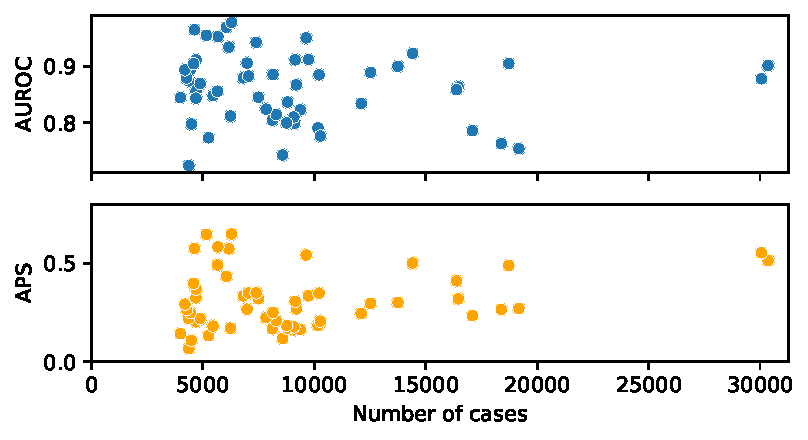
\includegraphics[width=0.9\linewidth]{img/chapter_3/behrt-performances.pdf}
    \end{center}
    \caption{BEHRT \citep{li2020behrt} performances for every diagnosis target.
      Number of positive cases is above 5000 for almost every disease.}
    \label{apd:fig:behrt_performances}
  \end{figure}


  A strong argument in favor of foundation models trained on EHRs is their
  ability to transfer well to downstream once pretrained. However, in most of the
  papers presenting these models, the number of cases used for the downstream
  tasks is out of reach for numerous medical applications. Table
  \ref{apd:table:foundation_model_nb_cases} shows the number of cases for
  downstream tasks of Med-BERT and CEHR-BERT. All tasks exceed 10,000 cases, a
  number of cases out of reach for the vast majority of healthcare centers. Figure
  \ref{apd:fig:behrt_performances} outlines the performances of BEHRT on every
  diagnosis. There is no clear trend that outlines better performances for higher
  number of cases. However, the number of cases is still greater than 5000 for
  almost all targeted diseases.

  Coupled to the current impossibility to share (and transfer) the weights of
  these models, this need for large downstream datasets is a strong limitation to
  their use in practice.


  \section{Review of computing resources for modern predictive models in healthcare}%
  \label{apd:computing_resources_review}

  The increasing architecture sizes of predictive models require appropriate
  computing infrastructures to pre-train and deploy those models. Table
  \ref{table:computing_resource_review} reviews the computing requirements for some
  of these modern predictive models. Computing resources for Large Language Models
  trained with clinical notes are greater than for EHR or claims models. Numbers
  are rarely provided at deployment , since they require smaller computing
  resources.


  \begin{table}[]
    \resizebox{\textwidth}{!}{%
      \begin{tabular}{llllllll}
        \toprule
        \begin{tabular}[c]{@{}l@{}}Data\\ Type\end{tabular}                                                                                                               &
        \begin{tabular}[c]{@{}l@{}}GPU  \\ number\end{tabular}                                                                                                            &
        GPU model                                                                                                                                                         &
        \begin{tabular}[c]{@{}l@{}}Training \\ time (hours)\end{tabular}                                                                                                  &
        Pretraining                                                                                                                                                       &
        \begin{tabular}[c]{@{}l@{}}Sample size\\ (millions)\end{tabular}                                                                                                  &
        Server details                                                                                                                                                    &
        Reference                                                                                                                                                           \\
        \hline
        Claims                                                                                                                                                            &
        4                                                                                                                                                                 &
        Nvidia V100                                                                                                                                                       &
        \textless{}24                                                                                                                                                     &
        No                                                                                                                                                                &
        43                                                                                                                                                                &
        72 CPU cores                                                                                                                                                      &
        \cite{beaulieu2021machine}                                                                                                                                          \\
        EHR                                                                                                                                                               &
        NA                                                                                                                                                                &
        \begin{tabular}[c]{@{}l@{}}Nvidia Titan Xp\end{tabular}                                                                                                           &
        NA                                                                                                                                                                &
        Yes                                                                                                                                                               &
        1.6                                                                                                                                                               &
        NA                                                                                                                                                                &
        \cite{li2020behrt}                                                                                                                                                  \\
        EHR                                                                                                                                                               &
        2                                                                                                                                                                 &
        \begin{tabular}[c]{@{}l@{}}Nvidia RTX \\ 20280 Ti\end{tabular}                                                                                                    &
        45                                                                                                                                                                &
        Yes                                                                                                                                                               &
        2.4                                                                                                                                                               &
        768 GB memory                                                                                                                                                     &
        \cite{pang2021cehr}                                                                                                                                                 \\
        EHR                                                                                                                                                               &
        1                                                                                                                                                                 &
        \begin{tabular}[c]{@{}l@{}}Nvidia V100\\ 32 GB\end{tabular}                                                                                                       &
        168                                                                                                                                                               &
        Yes                                                                                                                                                               &
        28                                                                                                                                                                &
        NA                                                                                                                                                                &
        \cite{rasmy2021med}                                                                                                                                                 \\
        Text                                                                                                                                                              &
        24                                                                                                                                                                &
        \begin{tabular}[c]{@{}l@{}}Nvidia A100\\ 40GB\end{tabular}                                                                                                        &
        504                                                                                                                                                               &
        Yes                                                                                                                                                               &
        0.39                                                                                                                                                              &
        \begin{tabular}[c]{@{}l@{}}Pre-training on NYU Langone \\ High-Performance Computing;\\ \\ Deployment on 128 GB RAM\\  servers with 2  RTX 3090 GPUs\end{tabular} &
        \cite{jiang2023health}                                                                                                                                              \\
        Text                                                                                                                                                              &
        992                                                                                                                                                               &
        Nvidia A100                                                                                                                                                       &
        144                                                                                                                                                               &
        Yes                                                                                                                                                               &
        2                                                                                                                                                                 &
        HiperGator-AI cluster                                                                                                                                             &
        \cite{yang2022gatortron}                                                                                                                                            \\
        \bottomrule
      \end{tabular}%
    }
    \vspace{1em}
    \caption{Computing resources for modern large scale predictive models.}
    \label{table:computing_resource_review}
  \end{table}

  \section{Detailed pipelines}\label{apd:pipelines}

  For all methods except demographics, the event features are the following
  structured events: billing codes (ICD-10), procedure codes (CCAM nomenclature),
  drugs administration (ATC7 nomenclature). Despite their high predictive
  potential, we did not consider biology since the number of events was too big
  for our memory capacity.

  \subsection{Demographics}\label{apd:pipelines:demographics}

  All static features correspond to the index visit of the task (T1=target stay,
  T2=first included stay, T3=???): age, gender, admission reason, discharge destination,
  type and value.

  The feature time of day was built as followed: morning between 7am and 12pm,
  afternoon between 12pm and 20pm and night between 20pm and 7am. This feature was
  mostly set at night, because almost all times are set to 22:00pm in our data
  extraction. More fine grained details should be available in the information
  system but were not communicated to us.

  \subsection{Count encoding}\label{apd:pipelines:count_encoding}

  Figure \ref{apd:fig:pipelines:count_encoding} details how counts and time decays
  are computed. During cross-validation, the explored decay parameters are:
  $\big[[0], [0, 1], [0, 7], [0, 30], [0, 90]\big]$.

  \begin{figure}
    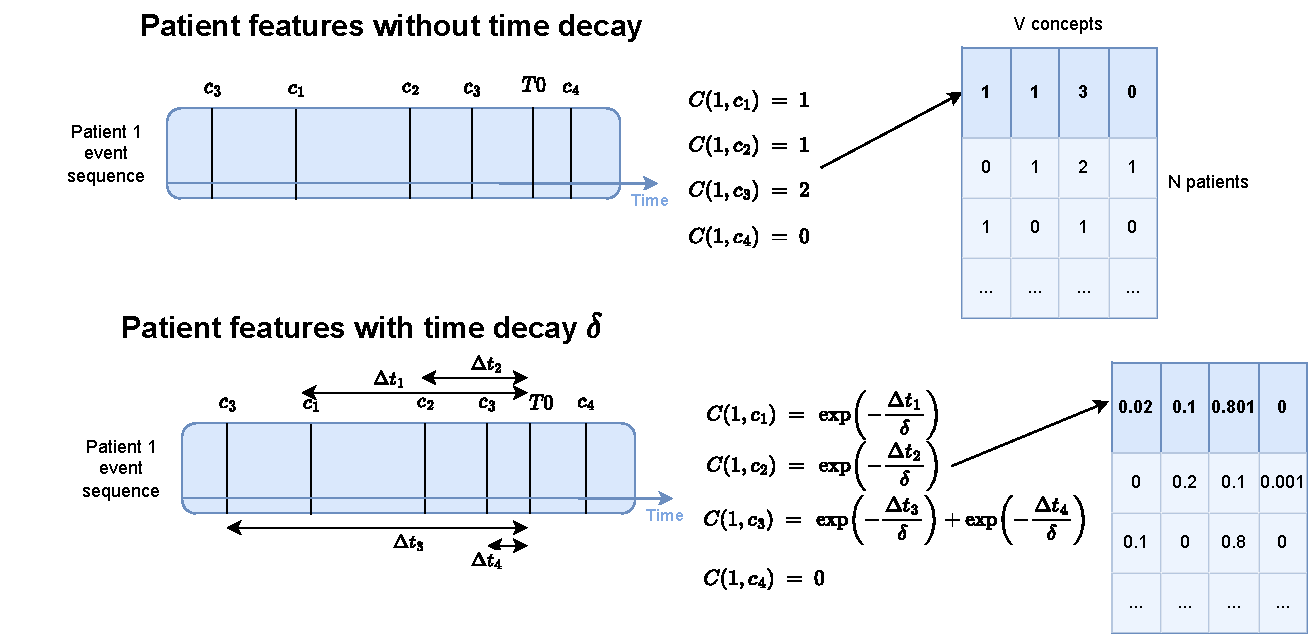
\includegraphics[width=0.9\textwidth]{img/chapter_3/patient_counter_with_decay.pdf}
    \caption{Count encoding procedure.}\label{apd:fig:pipelines:count_encoding}
  \end{figure}

  \subsection{Static Embeddings of event features}\label{apd:pipelines:static_embeddings}

  \paragraph{SVD-PPMI}\label{apd:medical_concept_embeddings:svdppmi} We recall the
  SVD-PPMI algorithm developed by \cite{beam2019clinical} and used for
  transferring phenotyping in \cite{hong2021clinical}.

  The algorithm takes a sequence of coded events as input and outputs vector
  representations. As shown in Figure \ref{fig:cooccurrence}, it builds a
  context window around every event $e=(i,t, c)$ , then updates the cooccurrence matrix for
  the corresponding medical code $P(c, c_j) \, \forall \, c_j \in Vocabulary$.

  \begin{figure}[htbp]
    \begin{center}
      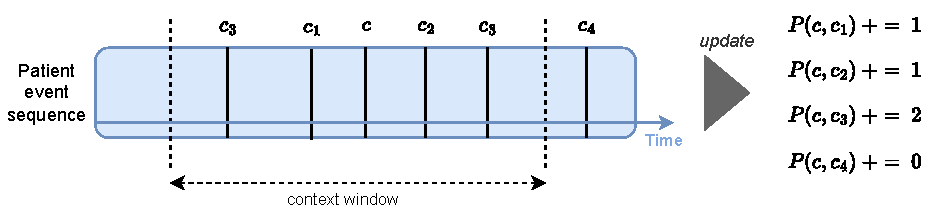
\includegraphics[width=0.9\linewidth]{img/chapter_3/cooccurrence.pdf}
    \end{center}
    \caption{The cooccurrence matrix is updated when two events occur in a
      specified time window.} \label{fig:cooccurrence}
  \end{figure}

  The PPMI matrix is then computed as the logged-shifted version of the
  cooccurrence matrix.
  \begin{equation}\label{eq:pmi}
    PMI(c_i, c_j) = log\frac{P(c_i, c_j)N}{P(c_i)P(c_j)}
  \end{equation}

  where $P(c_i)$ is the total count of the event $c_i$ and $N$ is the total count of events.

  \begin{equation}\label{eq:ppmi}
    PPMI = max(0, PMI - log(k))
  \end{equation}

  Finally, concept embeddings are recovered by SVD factorization and taking the
  mean of the context and target word matrix.

  \begin{equation}
    PPMI = U \cdot \Sigma \cdot V
  \end{equation}

  \begin{equation}
    embeddings = U_d \cdot \sqrt{\Sigma_d} + V_d \cdot \sqrt{\Sigma_d}
  \end{equation}

  Where the subscript $d$ denotates the restriction to the first $d$ components of
  the matrices.

  \paragraph{Aggregation of the static embbedings}

  Figure \ref{apd:fig:pipelines:static_embeddings_aggregation} details how the aggregation on a
  patient sequence is performed before feeding the vector to a scikit-learn estimator.

  \begin{figure}
    \centering
    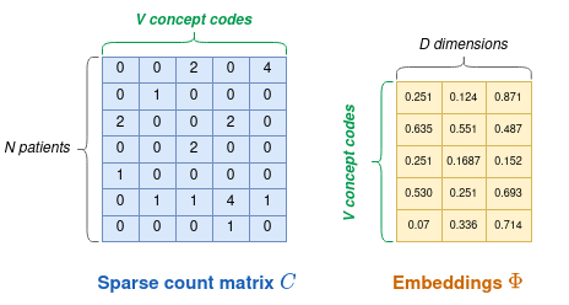
\includegraphics[width=0.8\textwidth]{img/chapter_3/static_embeddings_aggregation.png}
    \caption{Aggregation of the embeddings to yield one vector representing each
      patient sequence. The left blue matrix is the same as the one computed in
      the count encoding method. It is multiplied by the embedding matrix $\Phi$ either
      learned on the training set or transferred from the SNDS claims database.
    }\label{apd:fig:pipelines:static_embeddings_aggregation}
  \end{figure}

  \subsection{CEHR-BERT}\label{apd:pipelines:cehr_bert}

  CEHR-BERT is based on the original BERT architecture \citep{devlin2018bert}.
  \cite{pang2021cehr} modified previous transformers applied on EHR in two ways.
  They embed absolute and relative time with age of the patients, using a fourier
  transform of time numerical values. Secondly, they add the Visit Type Prediction
  objective. In addition to the usual sequence reconstruction task (masked
  language model) for concept embeddings, the model also tries to reconstruct the
  type of the visit associated with the masked concepts (inpatient,
  outpatient,emergency).

  \section{Experimental study}\label{apd:predictive_models:experimental_study}

  \subsection{Database description: two extractions from the Paris hospitals data warehouse}%
  \label{apd:database_description}

  We use two data extractions from the clinical data warehouse of the Greater
  Hospital of Paris (AP-HP) hosting routine care data from 38 hospitals formatted
  in the OHDSI OMOP format \citep{hripcsak2015observational}. The first extraction
  containing 200,000 randomly sampled patients, is used for the LOS
  (\ref{par:task_definitions:los}) and Prognosis
  (\ref{par:task_definitions:prognosis}) tasks. For the MACE task
  \ref{par:task_definitions:mace}, the number of case events --prevalence-- was
  lower than for the two other tasks, so we had to work on a bigger extraction
  containing 2.1 million patients. In both cases, raw data contained diagnoses and
  procedures billing codes, prescriptions and administrations of drugs,
  administrative information, laboratory results for inpatient only and clinical
  notes.

  We sessionize the visits to merge indices that are closer than one day into one
  unique stay. This avoids to consider transfers as two different hospitalizations.

  %
  \subsection{Tasks
    descriptions}\label{apd:tasks:population_selection}

  The Figure \ref{apd:fig:flowcharts} shows the selection flowcharts for the three tasks.

  \begin{figure}[!h]
    \centering
    \begin{subfigure}[b]{0.45\textwidth}
      \centering
      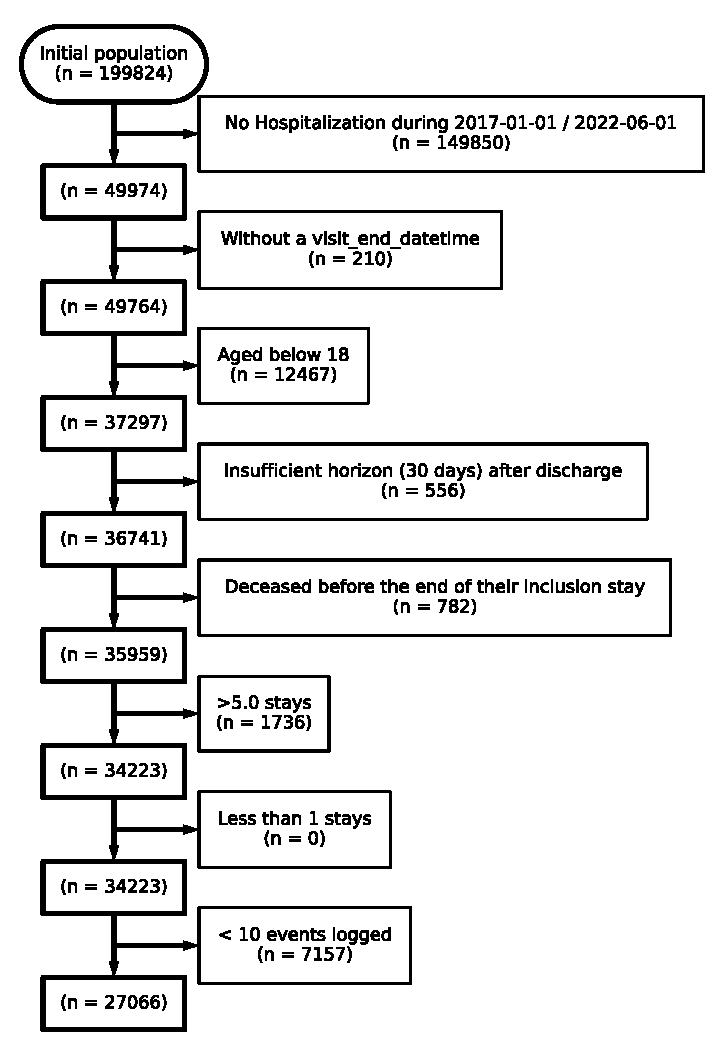
\includegraphics[width=\textwidth]{img/chapter_3/flowchart_t1_los.pdf}
      \caption{Selection flowchart for Length Of Stay interpolation task.}
      \label{apd:fig:flowchart_t1}
    \end{subfigure}
    \hfill
    \begin{subfigure}[b]{0.5\textwidth}
      \centering
      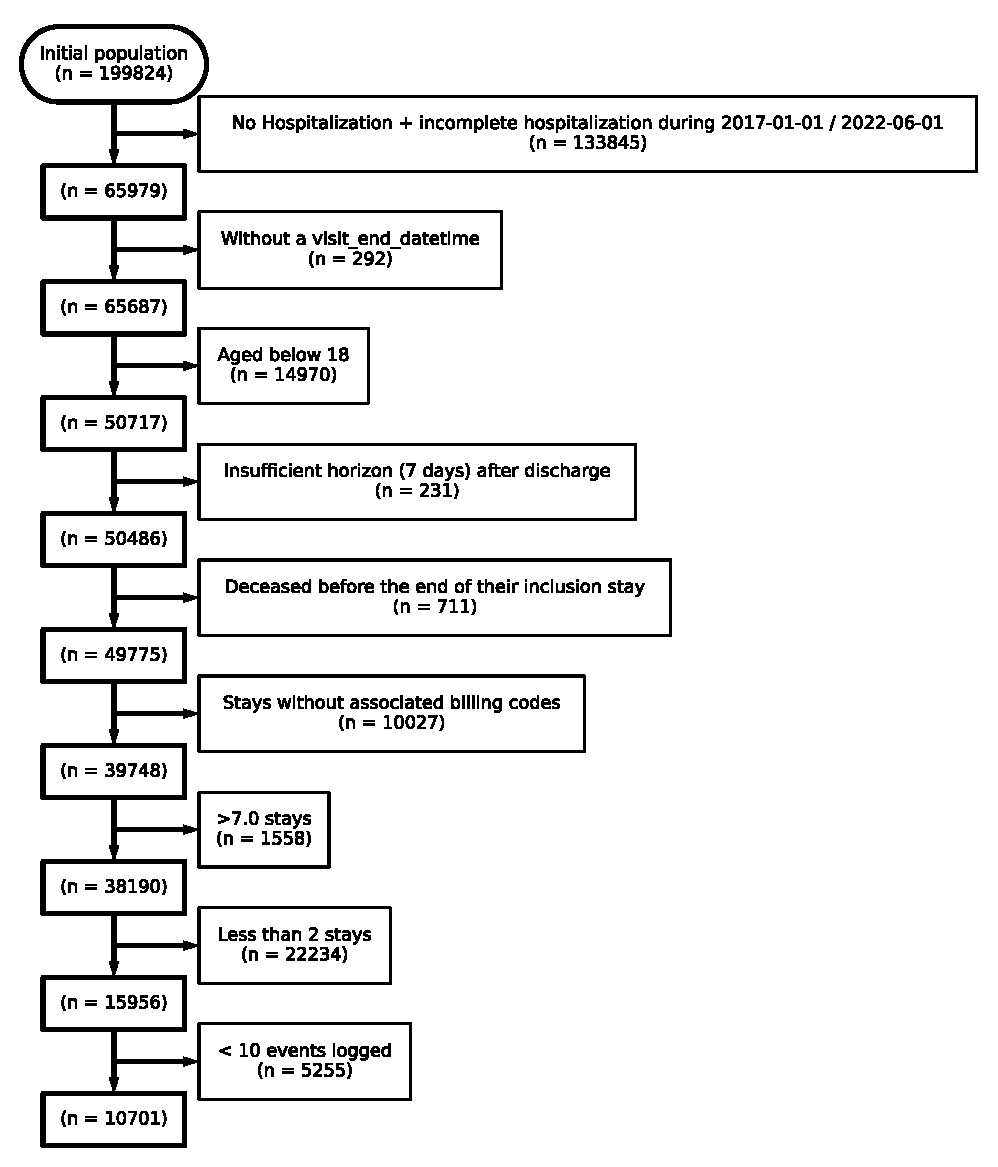
\includegraphics[width=1.1\textwidth]{img/chapter_3/flowchart_t2_icd10.pdf}
      \caption{Selection flowchart for ICD-10 chapter prediction task.}
      \label{apd:fig:flowchart_t2}
    \end{subfigure}
    \vfill
    \begin{subfigure}[b]{0.5\textwidth}
      \centering
      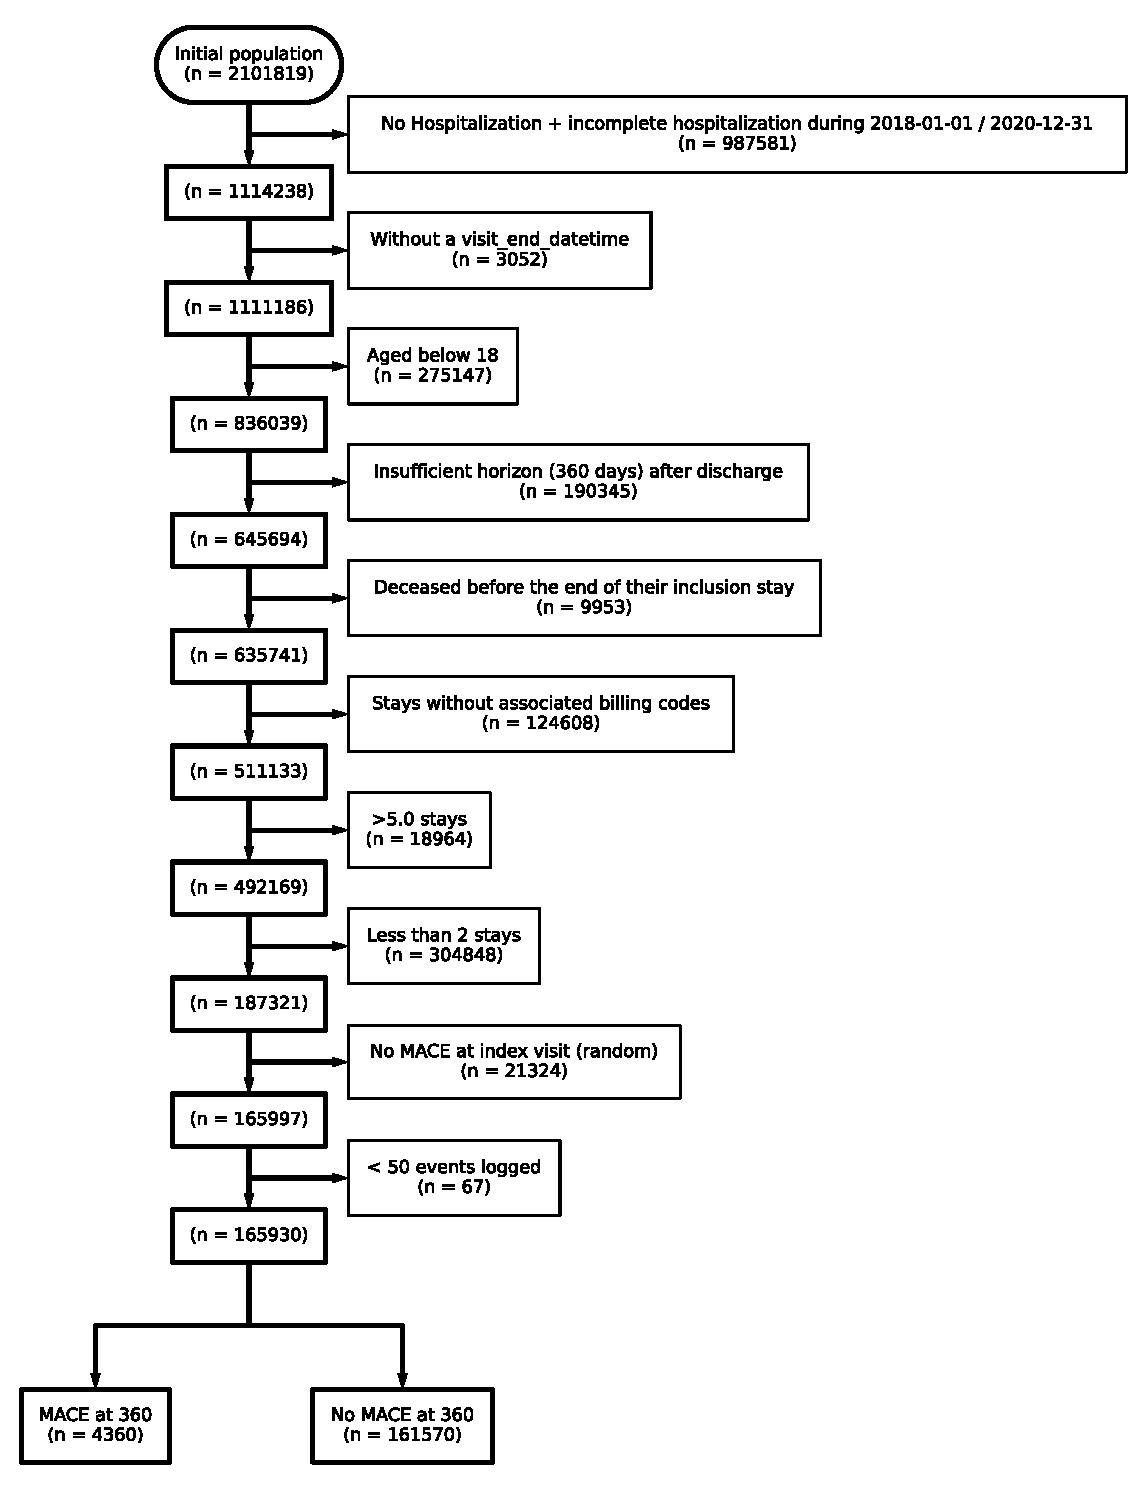
\includegraphics[width=1.1\textwidth]{img/chapter_3/flowchart_t3_mace.pdf}
      \caption{Selection flowchart for MACE prognosis.}
      \label{apd:fig:flowchart_t3}
    \end{subfigure}
    \caption{Selection flowcharts for the three tasks.}
    \label{apd:fig:flowcharts}
  \end{figure}

  \paragraph{LOS interpolation}\label{apd:task_details:los}

  The \emph{study period} was january 2017 to june 2022. The \emph{population at
    risk} are the patients aged above 18, with at least one hospitalization
  lasting at least 24 hours. Stays with in-hospital mortality are discarded. The
  \emph{index visit} is the first included visit for each individual. LOS is
  defined as a binary classification task for each index visit. The label is 0
  if the stay lasts less than 7 days and 1 if the stay lasts more than 7 days.
  The \emph{horizon} is the end of the index visit and the \emph{observation
    period} is the full index visit. This task is an interpolation since we
  classify the length of the stay with data from the whole stay.

  \paragraph{Prognosis task}\label{apd:task_details:prognosis}

  The study period was january 2017 to june 2022. The \emph{cohort}
  are the patients aged above 18, with at least two hospitalization (inpatient or
  outpatient). Stays with in-hospital mortality are discarded. The \emph{index
    stay} is defined as a random stay for each individual before its last stay. The
  \emph{horizon} is the beginning of the next stay and the \emph{observation
    period} is the full patient trajectory up to the end of the index visit.
  Prognosis is defined as a multi-label classification task. In the following stay
  after the index visit, for each of the 20 ICD10 chapters with a prevalence
  greater than 1\%, the label is 1 if the stay contains a diagnosis in this
  chapter, otherwise it is 0.

  \paragraph{Major Adverse Cardiovascular Events}\label{apd:task_details:mace}

  The study period was january 2018 to december 2020. The \emph{population at
    risk} are the patients aged above 18, with at least two hospitalization
  (inpatient or outpatient). \emph{The index visits} are for each patients a
  randomly selected stay without in-hospital mortality, with at least an
  \emph{horizon} of 12 months between the end of the stay and the end of the
  study period. The \emph{observation period} is the whole patient trajectory up
  to the end of the index visit. MACE is defined as a binary classification task.
  The label is 1 if a MACE billing code is observed (see Table
  \ref{apd:tasks:mace_codes}) and 0 otherwise. We used billing codes defined by
  \cite{bosco2021major} and complement them with other codes specific to the French healthcare
  system \cite{cnam2022_top_patho}.

  \begin{table*}[!tb]
    \resizebox*{\textwidth}{!}{
      \begin{tabular}{ll}
    \toprule
    Acute Myocardial Infarction           & I210, I211, I219, I220, I221, I229                           \\
    Unstable Angina                       & I200, I208, I209                                             \\
    Acute Heart Failure                   & I501, I5020, I5021, I5022, I5023, I5030, I5031, I5032, I5033 \\
    Acute Cerebrovascular Events (Stroke) & I60, I61, I62, I630, I631, I632, I633, I634, I64             \\
    Other codes                           & I24, I23                                                     \\
    \bottomrule
\end{tabular}

    } \caption{ICD10 codes used for MACE definition.}\label{apd:tasks:mace_codes}
  \end{table*}

  \subsection{Training procedure}\label{apd:evaluation_procedure}

  The temporal split was designed for the train/test ratio to be 0.8/0.2. This
  resulted in different split dates for each dataset. For LOS, training period
  covers 2017-01-01 to 2021-04-06 and test period covers 2021-04-07 to 2022-05-01.
  For Prognosis, train period covers 2017-01-01 to 2021-04-21 and test period
  covers 2021-04-22 to 2022-05-20. For MACE, train period covers 2018-01-01 to
  2019-08-11 and test period covers 2019-08-11 to 2020-01-05.

  Note that CEHR-BERT is also pre-trained on growing parts of the train
  set but only uses a validation set for stopping pretraining. Due to the high
  computing cost of transformers, we could not cross-validate its internal
  parameters.


  \section{Supplementary results for temporal split}\label{apd:temporal_split}

  \subsection{LOS interpolation}\label{apd:temporal_split:los}

  \begin{figure}[!h]
    \centering
    \includegraphics[width=\linewidth]{img/chapter_3/los/average_precision_score_performances.pdf}
    \caption{LOS average precision curve for different featurizers and estimators.
      The performances are averaged over 5 folds. The shaded area represents the
      standard deviation. The task performance seems to saturate at 98\% average
      precision for random forest and all featurizers but the demographics,
      suggesting that the Bayes error rate is reached. However, for lower sample
      regimes --below 12,500 patients, we see an advantage of static embeddings
      over event counts (both for logistic regression and random forest).}%
    \label{fig:los_auprc}
  \end{figure}



  \subsection{Prognosis}\label{apd:temporal_split:prognosis}

  \paragraph{Average Precision}

  Figure \ref{fig:prognosis_auprc} displays the area under the precision
  recall curve (average precision) averaged with equal weight for each chapter (Macro)
  and with the chapter prevalence as the weight (weighted).


  \begin{figure}[!h]
    \centering
    \begin{subfigure}[b]{1\textwidth}
      \caption{}\label{fig:prognosis_auprc_macro}
      \includegraphics[width=\linewidth]{img/chapter_3/prognosis/average_precision_score__c_macro.pdf}
    \end{subfigure}
    \vfill
    \begin{subfigure}[b]{1\textwidth}
      \caption{}\label{fig:prognosis_auprc_weighted}
      \includegraphics[width=\linewidth]{img/chapter_3/prognosis/average_precision_score__c_weighted.pdf}
    \end{subfigure}
    \caption{Prognosis average precisions average over chapters for different featurizers and
      estimators. The performances are averaged over 5 folds. The shaded area
      represents the standard deviation. The horizontal black lines display the
      naive baseline that predicts the previous stay codes for the target stay.
      Figure \ref{fig:prognosis_auprc_macro} average all chapter with equal weight
      whereas \ref{fig:prognosis_auprc_weighted} averages chapters by prevalences.
      Random forest have better performances. Count encoder outperform other
      featurizers, suggesting the importance of low count events that are smoothed
      out in embedding methods. Appendix \ref{apd:temporal_split:prognosis}
      details the results for each chapter and display Average Precision and Brier
      Score results.}%
    \label{fig:prognosis_auprc}
  \end{figure}


  \paragraph{Average precision scores for every ICD10 chapter}

  Figure \ref{fig:prognosis_average_precision_score__c_1} to
  \ref{fig:prognosis_average_precision_score__c_22} display AUPRC scores for every
  ICD10 chapters with respect to number of patients in the train set. Recall that
  contrary  to ROC AUC where the random baseline is 0.5, the random baseline for
  AUPRC is the prevalence of the target class.

  \def\icdchapterlist{21,4,9,18,5,2,6,11,13,14,10,19,3,1,7,22,12,20,15,17,8}
  \def\prognosispath{img/chapter_3/prognosis}
  \foreach \x in \icdchapterlist{%   
    \ifnum\x=16
      %
    \else
      \begin{figure}[htbp]
        \centering
        \includegraphics[width=\textwidth]{\prognosispath/average_precision_score__c_\x.pdf}%
        \caption{ICD10 chapter \x}\label{fig:prognosis_average_precision_score__c_\x}
      \end{figure}
    \fi
  }

  \paragraph{Prevalence results}\label{apd:prognosis_prevalences}


  Figure \ref{apd:fig:prognosis_prevalences_auprc_linear} shows the prevalence
  results for the Average precision curve and the linear estimator.

  Figure \ref{apd:fig:prognosis_prevalences_auroc_linear} shows the prevalence
  results for the ROC AUC curve and the linear estimator.

  Figure \ref{apd:fig:prognosis_prevalences_auroc} shows the prevalence results
  for the ROC AUC curve and the random forest estimator.



  \begin{figure}[!h]
    \centering
    \includegraphics[width=0.8\linewidth]{img/chapter_3/prognosis/prevalence_results__est_ridge_boxplot_roc_auc_score_xlog.pdf}
    \caption{Bigger target prevalences yield better ROC AUC. The different
      chapters are binned in prevalence bins. The estimator used for this plot is
      a penalized linear model trained on the full effective train set. Each box
      contour represents Q1-Q3 inter-quartile range.}%
    \label{apd:fig:prognosis_prevalences_auprc_linear}
  \end{figure}


  \begin{figure}[!h]
    \centering
    \includegraphics[width=0.8\linewidth]{img/chapter_3/prognosis/prevalence_results__est_ridge_boxplot_average_precision_score_xlog.pdf}
    \caption{ Bigger target prevalences yield better average precision. The different
      chapters are binned in prevalence bins. The estimator used for this plot
      is a penalized linear model trained on the full effective train set.}%
    \label{apd:fig:prognosis_prevalences_auroc_linear}
  \end{figure}


  \begin{figure}[!h]
    \centering
    \includegraphics[width=0.8\linewidth]{img/chapter_3/prognosis/prevalence_results__est_random_forests_boxplot_roc_auc_score_xlog.pdf}
    \caption{ Bigger target prevalences yield better ROC AUC. The
      different chapters are binned in prevalence bins. The estimator used for
      this plot is random forest trained on the full effective train set.}%
    \label{apd:fig:prognosis_prevalences_auroc}
  \end{figure}




  \subsection{MACE}\label{apd:temporal_split:mace}

  \section{Results for the geographic split}\label{apd:hospital_split}

  \subsection{Dataset split by hospital}

  To evaluate the geographic validity of our results, we proceed to a
  geographic split for train and test, according to hospitals. In the test set,
  the patients visited one of the following hospitals: Avicenne, Jean Verdier,
  Cochin, Ambroise Pare and Raymond Poincare-Berck. In the train set, patients
  visited another of the AP-HP 38 hospitals. Patients having a visit in both
  hospital groups were removed from both the train and test data. Figure
  \ref{apd:fig:hospital_split} shows the hospital cooccurrence matrix for
  patient populations.


  \begin{figure}[!h]
    \centering
    \includegraphics[width=\textwidth]{img/chapter_3/hospital_split_coocurrence_dice_score.pdf}
    \caption{Hospitals clustered by average euclidean distance in common patients
      from the LOS cohort. Scale in dice score: $2 \cdot |A \cap B| / (|A| + |B|)$. Test
      set hospitals appear in purple on the left.}\label{apd:fig:hospital_split}
  \end{figure}


  \subsection{Hospital split results}

  \paragraph{LOS interpolation}\label{apd:hospital_split:los}

  This task is saturated by the best machine learning models so we did not
  evaluate the transformer on it. Instead, we benchmarked the transfer from
  cui2vec embeddings, trained on american claims \citep{beam2019clinical}. To be
  fair to these embeddings, we restricted the vocabulary of medical codes to the
  common intersection of 2100 codes occurring both in cui2vec and in our dataset.
  The decay was set to 7 days (not cross-validated as in the main experiments).
  Figure \ref{apd:fig:hospital_split_los_decay7_roc_auc} shows all
  embeddings methods outperforming the count models.


  \begin{figure}[!h]
    \centering
    \includegraphics[width=\textwidth]{img/chapter_3/hospital_split_los_decay7_roc_auc.pdf}
    \caption{LOS task, transfer between hospitals with 2100 codes only, ROC AUC:
      The local, SNDS or cui2vec embeddings with forest and boosting are all
      equivalent. For logistic regression, the local embeddings remain the best
      performing method. We also compare the effect of reducing the dimension by applying a
      Singular Value Decomposition with 30 components kept. This increases a
      little bit the performance for logistic regression but decreases the performances of the
      other estimators.}\label{apd:fig:hospital_split_los_decay7_roc_auc}
  \end{figure}


  \paragraph{Prognosis}\label{apd:hospital_split:prognosis}

  Figure \ref{apd:fig:hospital_split_prognosis_roc_auc} shows the results on the
  prognosis task, with train/test split by hospital. We average the results for
  the 21 target diagnosis chapters: either with the same weight for each chapter
  (macro) or weighted by each chapter prevalence (weighted). The Random forest estimators
  with SNDS embeddings seem to be the best performing method. The transformer
  method begins to be competitive only with 8000 thousands patients in the train
  set. An interesting result is the performance of the naive method that predicts
  a diagnosis if it is present in the index visit (last stay before prediction
  target). It outperforms all other methods by a large margin, suggesting than
  ICD10 predictions might not be a useful predictive task. This result made us add
  the codes from the previous visit as new static feature to the prediction matrix
  in the main analysis.

  \begin{figure}[h!]
    \centering
    \begin{subfigure}[b]{\linewidth}
      \includegraphics[width=\linewidth]{img/chapter_3/hospital_split_prognosis_roc_auc_score__c_macro.pdf}
      \caption{}%
      \label{apd:fig:hospital_split_prognosis_roc_auc_macro}
    \end{subfigure}
    \vfill
    \begin{subfigure}[b]{\linewidth}
      \includegraphics[width=\linewidth]{img/chapter_3/hospital_split_prognosis_roc_auc_score__c_micro.pdf}
      \caption{}%
      \label{apd:fig:hospital_split_prognosis_roc_auc_weighted}
    \end{subfigure}
    \caption{Prognosis task, transfer between hospitals, weighted average (by chapter
      prevalence) and macro average ROC AUC: The black vertical line shows the
      results from predicting the next diagnoses if they appear in the last visits
      in the observation period.}%
    \label{apd:fig:hospital_split_prognosis_roc_auc}
  \end{figure}

  \section{Vibration study on the effects of the decay}
  \label{apd:vibration_study_decay}

  Using the LOS task, we investigated if the decay hyperparameter played an
  important role in the performances of the different pipelines. We evaluated this
  vibration analysis on a randomly chose train set (no temporal or hospital data
  shift). Figure \ref{apd:fig:vibration_decay} shows the big impact of different
  decay hyperparameters on ROC AUC. This led us to cross-validate the decays in
  the main analyses. Interestingly, concatenating multiple decays only had a
  significant impact on the count pipelines.

  \begin{figure}[!h]
    \centering
    \includegraphics[width=\textwidth]{img/chapter_3/random_split_los_decay_vibration_roc_auc.pdf}
    \caption{LOS task, random test set, ROC AUC, estimator is random forest:
      Concatenating a one day decay add 10 points of ROC AUC to the embedding
      pipeline.}\label{apd:fig:vibration_decay}
  \end{figure}


  \section{Medical concept embeddings}\label{apd:medical_concept_embeddings}

  \subsection{Previous work and motivation}\label{apd:medical_concept_embeddings:previous_work}

  Building on a formulation of word2vec \citep{mikolov2013distributed} as the
  factorization of the Positive Pointwise Information Matrix --PPMI eq.
  \ref{eq:ppmi}--, \citet{beam2019clinical} built medical concept embeddings from
  both text and structured data. These embeddings are non-contextual, meaning that
  they do not take into account the full sequence of event at the time of
  inference. These make them less powerful than contextual embeddings such as the ones from
  the transformer-based models \citep{li2020behrt, rasmy2021med, pang2021cehr}.

  However, the information at the basis of the non-contextual embeddings is a
  sharable aggregated data: the cooccurrence matrix. The easy creation and
  exchange of medical concept embeddings opens a wide range of applications that
  efficiently pulls data from multiple sites, overcoming both the heterogeneity of
  the data, and the administrative barriers to access individual patient data.
  Transferring these dense representations of healthcare events to specific
  low-sampled cohorts might provide \textit{efficient} pretrained data
  representations even in setups where very few patients are available.


  \subsection{Background on medical concept embeddings for prediction}%
  \label{apd:background_static_embeddings}%

  Only few works have studied the transfer capabilities of clinical concept
  embeddings for relevant prognosis tasks. None of them studied how such
  representations can be used in a combination with traditional machine learning
  techniques such as random forests or logistic regressions.

  \cite{huang2018privacy} used the same embeddings method on the two EHR in MIMIC,
  fusing them with Procruste. Utility is evaluated on diagnoses prediction tasks,
  using Patient Diagnosis Projection Similarity, top-K cosine distance between a
  temporally weighted average of the embedding for a given patient and the
  diagnoses embeddings. They show that Procruste fused embeddings are almost as
  performant (measured with ROC-AUC) as embeddings derived from the two databases.

  \cite{hong2021clinical} used SVD-PPMI factorization on two databases. They
  evaluated the utility of embeddings on a phenotyping downstream task for eight
  diseases: coronary artery disease (CAD), type I diabetes mellitus (T1DM), type
  II diabetes mellitus (T2DM), depression, rheumatoid arthritis (RA), multiple
  sclerosis (MS), Crohn's disease (CD) and ulcerative colitis (UC). They did not
  evaluate them for predictive tasks, only for differential diagnosis.

  \cite{xiang2019time} fine-tuned a LSTM on top of different medical concept
  representations (FastText \citep{bojanowski2017enriching}, SVD-PPMI or Skip-Gram
  with a time context window \citep{beam2019clinical} and ), for heart failure
  (11.7\% prevalence) reaching respectively for each representation 84.9, 82.4
  and 85.4 ROC AUC.

  \subsection{Embeddings implementation}\label{apd:medical_concept_embeddings:implementation}

  We published event2vec \footnote{\url{https://gitlab.com/strayMat/event2vec/}},
  a python package to quickly build medical concept embeddings using the SVD-PPMI
  algorithm \cite{beam2019clinical, levy2014neural}. Our package proposes two
  backends for the computation of this cooccurrence matrix: pandas for small
  datasets (ten thousand of patients), spark for big datasets
  \citep{salloum2016big}.

  \subsection{Qualitative assessment of the embeddings}

  Figure \ref{tsne_plots} displays 2D Tsne projections \cite{van2008visualizing}
  of the embeddings. Clear groups of pathologies has been recovered by the
  algorithm. Table \ref{table:embedding_nn} shows the ten closest neighbors of the
  \textit{Diabete type 1 with acidosis} concept for each dataset (by cosine
  distance), reflecting discrepancies between both dataset for this billing code.
  Interactive Tsne plots and full embeddings (SNDS only) are available on our
  gitlab repository
  \footnote{\url{https://gitlab.com/strayMat/event2vec/-/tree/main/data/results/}}.

  \begin{figure}[h]
    \centering
    \begin{subfigure}[b]{0.48\linewidth}
      \centering
      \caption{AP-HP}
      \includegraphics[width=\linewidth]{img/chapter_3/aphp2vec_annotated.png}
      \label{fig:tsne_plots:aphp}
    \end{subfigure}
    \hfill
    \begin{subfigure}[b]{0.48\linewidth}
      \centering
      \caption{SNDS}
      \includegraphics[width=\linewidth]{img/chapter_3/snds2vec_annotated.png}
      \label{fig:tsne_plots:snds}
    \end{subfigure}

    \caption{TSNE projection of medical event embeddings. Each point is a
      projection in 2D of the embedded vector for a given medical concept: a) in
      the AP-HP Clinical Data Warehouse (200, 000 random patients extractions), b)
      in the French Medical Claims (SNDS). Colors correspond to different medical
      vocabularies: drugs in green, billing diagnoses in blue, billing procedures
      in red, biology in pink (different vocabulary for AP-HP and SNDS), general
      practitioner (GP) activity in yellow. Interactive versions of these plots
      are available at:
      \url{https://straymat.gitlab.io/event2vec/visualizations.html}}
    \label{tsne_plots}
  \end{figure}

  \begin{table}
    \resizebox*{\textwidth}{!}{
      \begin{tabular}{llllr}
        \toprule
        Concept code & Concept label
                     & medical vocabulary                                                                                     & similarity                 \\
        \midrule
        I210         & Acute myocardial infarction
                     & ICD10:diagnosis                                                                                        & 1.000000                   \\
        I25          & Chronic ischemic heart disease                                                                         & ICD10:diagnosis & 0.491964 \\
        DDAF006      & \begin{tabular}[c]{@{}l@{}}Intraluminal dilatation of a \\coronary vessel with stenting\end{tabular}   & CCAM:procedures & 0.459349 \\
        DDQJ001      & \begin{tabular}[c]{@{}l@{}}Intra-arterial coronary ultrasound\\ and/or Doppler ultrasound\end{tabular} & CCAM:procedures & 0.455709 \\
        B01AC22      & Prasugrel                                                                                              & ATC7:drugs      & 0.426467 \\
        C03DA04      & Eplerenone                                                                                             & ATC7:drugs      & 0.385482 \\
        TNS          & Nicotine replacement therapy                                                                           & NGAP:GP         & 0.399372 \\
        SRA          & Resuscitation supplement                                                                               & NGAP:GP         & 0.392237 \\
        1526         & Creatine phosphokinase                                                                                 & NABM:biology    & 0.385801 \\
        521          & Lactate deshydrogenase (LDH)                                                                           & NABM:biology
                     & 0.315254                                                                                                                            \\
        \bottomrule
      \end{tabular}
    }
    \caption{Two closest concepts for each vocabulary for the medical concept I210
      of Transmural infarction with the claims SNDS embeddings. Prasugrel is a
      medication used to prevent formation of blood clots. Eplerenone is an
      aldosterone antagonist type of potassium-sparing diuretic that is used to
      treat chronic heart failure and high blood pressure. Creatine phosphokinase
      used to be determined specifically in patients with chest pain. Because
      Lactate deshydrogenase is released during tissue damage, it is a
      marker of common injuries and disease such as heart failure}%
    \label{table:embedding_nn}
  \end{table}



  \chapter{Chapter \ref{chapter:causal_tuto}}\label{apd:causal_tuto}

  \section{Motivating example: Failure of predictive models to predict mortality
    from pretreatment variables}%
  \label{apd:motivating_example}%

  To illustrate how machine learning frameworks can fail to inform decision
  making, we present a motivating example from MIMIC-IV. Using the same
  population and covariates as in the main analysis (described in Table
  \ref{apd:table:albumin_for_sepsis:table1_complete}), we train a predictive
  model for 28-day mortality. We split the data into a training set (80\%) and a
  test set (20\%). The training set uses the last measurements from the first 24
  hours, whereas the validation set only uses the last measurements before the
  administration of crystalloids. We split the train set into a train and a
  validation set. We fit a HistGradientBoosting classifier
  \footnote{\url{https://scikit-learn.org/stable/modules/ensemble.html\#histogram-based-gradient-boosting}}
  on the train set and evaluate the performance on the validation set and on the
  test set. We see good area under the Precision-recall curve (PR AUC) on the
  validation set, but a deterioration of 10 points on the test set (Figure
  \ref{apd:fig:motivating_example_pr_auc}). The same is seen in Figure
  \ref{apd:fig:motivating_example_roc_auc} when measuring performance with Area
  Under the Curve of the Receiving Operator Characteristic (ROC AUC). In the
  contrary, a model trained on pre-treatment features yield competitive
  performances. This failure illustrates well the shortcuts on which predictive
  models could rely to make predictions. A clinically useful predictive model
  should support decision making --in this case, addition of albumin to
  crystalloids-- rather than maximizing predictive performance. In this example,
  causal thinking would have helped to identify the bias introduced by
  post-treatment features. In fact, these features should not be included in a
  causal analysis since they are post-treatment colliders.

  \begin{figure}[!h]
    \begin{subfigure}{\linewidth}
      \centering
      \includegraphics[width=0.9\linewidth]{img/chapter_4/predictive_failure__pr_auc.pdf}
      \caption{}\label{apd:fig:motivating_example_pr_auc}
    \end{subfigure}
    \hfill
    \begin{subfigure}{\linewidth}
      \centering
      \includegraphics[width=0.9\linewidth]{img/chapter_4/predictive_failure__roc_auc.pdf}
      \caption{}\label{apd:fig:motivating_example_roc_auc}
    \end{subfigure}
    \caption{Failure to predict 28-day mortality from a model fitted on
      pre-treatment variables. The model is trained on the last features from
      the whole stay and tested on two validation sets: one with all stay
      features and one with last features before crystalloids administration
      (Pre-treatment only). The all-stay model performance markedly decreases in
      the pre-treatment only dataset.}\label{apd:fig:motivating_example}
  \end{figure}

  \section{Estimation of Treatment effect with MIMIC data}\label{apd:ate_on_mimic}

  We searched for causal inference studies in MIMIC using PubMed and Google
  scholar with the following search terms ((MIMIC-III OR MIMIC-IV) AND (causal
  inference OR treatment effect)). We retained eleven treatment effect studies
  clearly following the PICO framework:  \begin{itemize}

    \item \cite{liu2021effects} studied the effect of \textcolor{I}{High-flow
            nasal cannula oxygen (HFNC)} against \textcolor{C}{noninvasive
            mechanical ventilation} on \textcolor{P}{801 patients with hypoxemia
            during ventilator weaning} on \textcolor{O}{28-day mortality}. They
          used propensity score matching, and found non-negative effects as
          previous RCTs reported -- though those were focused on reintubation as the
          main outcome \citep{stephan2015high, hernandez2016effect}.

    \item \cite{yarnell2023oxygenation} studied the effect of \textcolor{I}{lower hypoxemia} vs \textcolor{C}{higher
          hypoxemia thresholds for the initiation of invasive ventilation} (defined with saturation-to-inspired oxygen ratio (SF)) for
          \textcolor{P}{3,357 patients from MIMIC receiving inspired oxygen fraction >= 0.4} on \textcolor{O}{28-day
            moratlity}. Using bayesian G-computation (time-varying treatment model with
          gaussian process and outcome-model with BART, taking the treatment model as
          entry), they found protective effects for initialization at low hypoxemia.
          However, when externally validation their findings in the AmsterdamUMCdb dataset,
          they found the highest mortality probability for patients with low hypoxemia.
          Authors concluded that their model was heavily dependent on clinical context
          and baseline caracteristics. There might be some starting-time bias in this study since it is really close

    \item \cite{hsu2015association} studied the effect of \textcolor{I}{indwelling
            arterial catheters (IACs)} vs \textcolor{C}{non-IAC} for
          \textcolor{P}{1,776 patients who are mechanically ventilated and did
            not require vasopressor support} on \textcolor{O}{28-day mortality}.
          They used propensity score matching and found no effect. A notebook based on google cloud access to MIMIC-IV
          replicating the study is available \href{https://github.com/alistairewj/mimic-iv-aline-study/blob/main/mimic_iv_aline.ipynb}{here}.

    \item \cite{feng2018transthoracic} studied the effect of
          \textcolor{I}{transthoracic echocardiography} vs \textcolor{C}{no
            intervention} for \textcolor{P}{6,361 patients with sepsis} on
          \textcolor{O}{28-day mortality}. They used IPW, PSM, g-formula and a
          doubly robust estimation. The propensity score was modeled with boosting
          and the outcome model with a logistic regression. They
          found a significant positive reduction of mortality (odd ratio 0.78, 95\% CI 0.68-0.90).
          \href{https://github.com/nus-mornin-lab/echo-mimiciii}{Study code is
            open source}.

    \item \cite{gani2023structural} studied the effect of \textcolor{I}{liberal
            --target SpO2 greater than 96\%--} vs \textcolor{C}{conservative
            oxygenation --target SpO2 between 88-95\%--} in \textcolor{P}{4,062
            mechanically ventilated patients} on \textcolor{O}{90-day mortality}.
          They found an advantage of the liberal strategy over liberal
          (ATE=0.13) by adjusting on age and apsii. This is not consistent with
          previous RCTs where no effects have been reported \citep{panwar2016conservative, mackle2019conservative}.

    \item \cite{shahn2020fluid} studied the effect of \textcolor{I}{fluid-limiting
            treatment --caped between 6 and 10 L--} vs \textcolor{C}{no cap on
            fluid administration} strategies for \textcolor{P}{1,639 sepsis
            patients} on \textcolor{O}{30 day-mortality}. Using a dynamic Marginal
          Structural Model with IPW, they found a protective effect of
          fluid-limitation on ATE -0.01 (95\%CI -0.016, -0.03). This is somehow
          concordant with the RIFTS RCT that found no effect of fluid limitation
          \citep{corl2019restrictive} and two previous meta-analyses
          \citep{malbrain2014fluid,meyhoff2020lower}.

    \item \cite{chinaeke2021impact} studied the effect of \textcolor{I}{statin use
            prior to ICU admission} vs \textcolor{C}{absence of pre-ICU
            prescription} for \textcolor{P}{8,200 patients with sepsis} on
          \textcolor{O}{30-day mortality}. Using AIPW (no estimator reported)
          and PSM (logistic regression), they found a decrease on mortality (ATE
          -0.039, 95\%CI -0.084, -0.026). This partly supports previous
          findings in Propensity Matching bases observational studies
          \citep{lee2017preadmission,kyu2019preadmission}. But all RCTs
          \citep{national2014rosuvastatin, singh2017effects} found no improvement for sepsis (not
          pre-admission administration though). The \cite{wan2014effect}
          meta-analysis concludes that there is lack of evidence for the use of
          statins in sepsis with inconsistent results between RCTs (no effect)
          and observational studies (protective effect).
    \item \cite{adibuzzaman2019323} studied the effect of \textcolor{I}{higher} vs
          \textcolor{C}{lower positive end-expiratory pressures (PEEP)} in
          \textcolor{P}{1,411 patients with Acute Respiratory Distress Syndrome
            (ARDS) syndrome} on \textcolor{O}{30 day mortality}. Very few details on
          the methods were reported, but they found a protective effect for higher PEEP
          consistent results from a target trial \citep{national2004higher}.
    \item \cite{adibuzzaman2019323} also studied the effect of \textcolor{I}{early
            use of a neuromuscular blocking agent } vs \textcolor{C}{placebo} in
          \textcolor{P}{752 patients moderate-severe ARDS} on \textcolor{O}{30
            day mortality}. Very few details on the methods were reported, but they found a
          protective effect for the use of a neuromuscular blocking agent,
          consistent with the results from a target trial
          \citep{papazian2010neuromuscular}.
    \item \cite{zhou2021early} studied the administration of \textcolor{I}{a
            combination of albumin within the first 24-h after crystalloids} vs
          \textcolor{C}{crystalloids alone} for \textcolor{P}{6,641 patients
            with sepsis} on \textcolor{O}{28-day mortality}. Using PSM, they found
          protective effect of combination on mortality, but insist on the
          importance of initialization timing. This is consistent with \cite{xu2014comparison}, who
          found a non-significant trend
          in favor of albumin used for severe sepsis patients and a significant
          reduction for septic shock patients, both on 90-day mortality. These
          results are aligned with \cite{caironi2014albumin} that found no effect
          for severe sepsis patient but positive effect for septic shock patients.
    \item \cite{wang2023early} studied \textcolor{I}{early enteral nutrition (EN)
            --<=53 ICU admission hours--} vs \textcolor{C}{delayed EN} for
          \textcolor{P}{2,364 patients with sepsis and EN} on
          \textcolor{O}{acute kidney injury}. With PSM, IPW and g-formula
          (logistic estimator each time), they found a protective effect
          (OR 0.319, 95\%CI 0.245, 0.413) of EEN.
  \end{itemize}

  These eleven studies mainly used propensity score matching (6) and IPW (4), two of
  them used Double robust methods, and only one included a non-linear estimator in
  either the outcome or the treatment model. None of them performed a vibration
  analysis on the confounders selection or the feature transformations. They have a
  strong focus on sepsis patients. Only four of them found concordant results with
  previous RCTs \citep{liu2021effects,shahn2020fluid,adibuzzaman2019323}.

  \section{Target trials proposal suitable to be replicated in MIMIC}\label{apd:target_trials}

  \cite{guzmanopen} suggested the creation of a causal inference database based
  on MIMIC with a list of replicable RCTs, which has not been
  accomplished yet. We reviewed the following RCTs, which could be replicated within the MIMIC-IV
  database. Table \ref{apd:table:emulated_trials_populations} details the sample
  sizes of the eligible, control and treated populations for the identified RCTs.


  \begin{table}[!h]
    \resizebox{\textwidth}{!}{%
      \begin{tabular}{|l|l|l|l|l|l|}
        \hline
        \textbf{Trial name}                                                                                                                                                                                                                                                                                                                                    &
        \textbf{Criteria description}                                                                                                                                                                                                                                                                                                                          &
        \textbf{\begin{tabular}[c]{@{}l@{}}Number of \\ patients\end{tabular}}                                                                                                                                                                                                                                                                                 &
        \textbf{\begin{tabular}[c]{@{}l@{}}Criteria \\ status\end{tabular}}                                                                                                                                                                                                                                                                                    &
        \textbf{Implemented}                                                                                                                                                                                                                                                                                                                                   &
        \textbf{\begin{tabular}[c]{@{}l@{}}Meta-analysis or \\ target RCT reference\end{tabular}}                                                                                                                                                                                                                                                                                                                                                                                                    \\ \hline
        \multirow{3}{*}{\begin{tabular}[c]{@{}l@{}}Fludrocortisone \\ combination for sepsis\end{tabular}}                                                                                                                                                                                                                                                     &
        \begin{tabular}[c]{@{}l@{}}Septic shock defined by the sepsis-3 criteria, \\ first stay, over 18, not deceased during first 24 hours of ICU\end{tabular}                                                                                                                                                                                               &
        28,763                                                                                                                                                                                                                                                                                                                                                 &
        \begin{tabular}[c]{@{}l@{}} target\\population\end{tabular}                                                                                                                                                                                                                                                                                            &
        \ding{51}                                                                                                                                                                                                                                                                                                                                              &
        \begin{tabular}[c]{@{}l@{}} \citep{yamamoto2020hydrocortisone} \end{tabular}                                                                                                                                                                                                                                                                                                                                                                                                                 \\ \cline{2-6}
                                                                                                                                                                                                                                                                                                                                                               &
        Hydrocortisone administred and sepsis                                                                                                                                                                                                                                                                                                                  &
        1,855                                                                                                                                                                                                                                                                                                                                                  &
        control                                                                                                                                                                                                                                                                                                                                                &
        \ding{51}                                                                                                                                                                                                                                                                                                                                              &
        \\ \cline{2-6}
                                                                                                                                                                                                                                                                                                                                                               &
        Both corticoides administered and sepsis                                                                                                                                                                                                                                                                                                               &
        153                                                                                                                                                                                                                                                                                                                                                    &
        intervention                                                                                                                                                                                                                                                                                                                                           &
        \ding{51}                                                                                                                                                                                                                                                                                                                                              &
        \\ \hline
        \multirow{3}{*}{\begin{tabular}[c]{@{}l@{}}High flow \\ oxygen therapy\\ for hypoxemia\end{tabular}}                                                                                                                                                                                                                                                   &
        \begin{tabular}[c]{@{}l@{}}Over 18, hypoxemia 4 h before planed extubation \\ (PaO2, FiO2) $\leq$ 300 mmHg), and either High Flow \\ Nasal Cannula (HFNC) or Non Invasive Ventilation (NIV)\end{tabular}                                                                                                                                               &
        801                                                                                                                                                                                                                                                                                                                                                    &
        \begin{tabular}[c]{@{}l@{}} target\\population\end{tabular}                                                                                                                                                                                                                                                                                            &
        \ding{55}                                                                                                                                                                                                                                                                                                                                              &
        \begin{tabular}[c]{@{}l@{}} \citep{stephan2015high}\end{tabular}                                                                                                                                                                                                                                                                                                                                                                                                                             \\ \cline{2-6}
                                                                                                                                                                                                                                                                                                                                                               &
        Eligible hypoxemia and HFNC                                                                                                                                                                                                                                                                                                                            &
        358                                                                                                                                                                                                                                                                                                                                                    &
        intervention                                                                                                                                                                                                                                                                                                                                           &
        \ding{55}                                                                                                                                                                                                                                                                                                                                              &
        \\ \cline{2-6}
                                                                                                                                                                                                                                                                                                                                                               &
        Eligible hypoxemia and NIV                                                                                                                                                                                                                                                                                                                             &
        443                                                                                                                                                                                                                                                                                                                                                    &
        control                                                                                                                                                                                                                                                                                                                                                &
        \ding{55}                                                                                                                                                                                                                                                                                                                                              &
        \\ \hline
        \multirow{3}{*}{\begin{tabular}[c]{@{}l@{}}Routine oxygen for  \\ myocardial infarction\end{tabular}}                                                                                                                                                                                                                                                  &
        \begin{tabular}[c]{@{}l@{}}Myocardial infarction without hypoxemia at admission:\\ \\ - Myocardial infarction defined with ICD9-10 codes, \\  first stay, over 18, not deceased during first 24 hours of ICU\\ \\ - Hypoxemia during first 2 hours defined as either  \\ (PaO2/FiO2) $leq$ 300mmHg OR SO2 $leq$ 90  \\  OR SpO2 $\leq$ 90\end{tabular} &
        3,379                                                                                                                                                                                                                                                                                                                                                  &
        \begin{tabular}[c]{@{}l@{}}target\\population\end{tabular}                                                                                                                                                                                                                                                                                             &
        \ding{51}                                                                                                                                                                                                                                                                                                                                              &
        \begin{tabular}[c]{@{}l@{}} \citep{hofmann2017oxygen}, \\ \citep{stewart2021high} \end{tabular}                                                                                                                                                                                                                                                                                                                                                                                              \\ \cline{2-6}
                                                                                                                                                                                                                                                                                                                                                               &
        \begin{tabular}[c]{@{}l@{}}Myocardial infarction without hypoxemia at admission AND \\ Supplemental Oxygen OR Non Invasive Vent\end{tabular}                                                                                                                                                                                                           &
        1,901                                                                                                                                                                                                                                                                                                                                                  &
        intervention                                                                                                                                                                                                                                                                                                                                           &
        \ding{51}                                                                                                                                                                                                                                                                                                                                              &
        \\ \cline{2-6}
                                                                                                                                                                                                                                                                                                                                                               &
        \begin{tabular}[c]{@{}l@{}}Myocardial infarction without hypoxemia at admission AND\\ no ventilation of any kind during first 12 hours\end{tabular}                                                                                                                                                                                                    &
        605                                                                                                                                                                                                                                                                                                                                                    &
        control                                                                                                                                                                                                                                                                                                                                                &
        \ding{51}                                                                                                                                                                                                                                                                                                                                              &
        \\ \hline
        \multirow{3}{*}{\begin{tabular}[c]{@{}l@{}}Prone positioning \\ for ARDS\end{tabular}}                                                                                                                                                                                                                                                                 &
        \begin{tabular}[c]{@{}l@{}}Acute Respiratory Distress Syndrome (ARDS) during \\ the first 12 hours defined as (PaO2,FiO2) $leq$ 300mmHg, \\ first stay, over 18, not deceased during 24 hours of ICU\end{tabular}                                                                                                                                      &
        11506                                                                                                                                                                                                                                                                                                                                                  &
        \begin{tabular}[c]{@{}l@{}}trial\\ population\end{tabular}                                                                                                                                                                                                                                                                                             &
        \ding{51}                                                                                                                                                                                                                                                                                                                                              &
        \citep{munshi2017prone}                                                                                                                                                                                                                                                                                                                                                                                                                                                                      \\ \cline{2-6}
                                                                                                                                                                                                                                                                                                                                                               &
        Prone positioning and ARDS                                                                                                                                                                                                                                                                                                                             &
        547                                                                                                                                                                                                                                                                                                                                                    &
        intervention                                                                                                                                                                                                                                                                                                                                           &
        \ding{51}                                                                                                                                                                                                                                                                                                                                              &
        \\ \cline{2-6}
                                                                                                                                                                                                                                                                                                                                                               &
        Supline position and no prone position                                                                                                                                                                                                                                                                                                                 &
        10,904                                                                                                                                                                                                                                                                                                                                                 &
        control                                                                                                                                                                                                                                                                                                                                                &
        \ding{51}                                                                                                                                                                                                                                                                                                                                              &
        \\ \hline
        \multirow{3}{*}{NMBA for ARDS}                                                                                                                                                                                                                                                                                                                         &
        \begin{tabular}[c]{@{}l@{}}ARDS during the first 12 hours defined as \\ (PaO2,FiO2) $leq$ 300mmHg, first stay, \\ over 18, not deceased during 24 hours of ICU\end{tabular}                                                                                                                                                                            &
        11,506                                                                                                                                                                                                                                                                                                                                                 &
        \begin{tabular}[c]{@{}l@{}}trial\\ population\end{tabular}                                                                                                                                                                                                                                                                                             &
        \ding{51}                                                                                                                                                                                                                                                                                                                                              & \begin{tabular}[c]{@{}l@{}} \citep{papazian2010neuromuscular}, \\ \citep{ho2020neuromuscular} \end{tabular}
        \\ \cline{2-6}
                                                                                                                                                                                                                                                                                                                                                               &
        \begin{tabular}[c]{@{}l@{}}Neuromuscular blocking agent  (NBMA) as cisatracurium \\ injections during the stay.\end{tabular}                                                                                                                                                                                                                           &
        709                                                                                                                                                                                                                                                                                                                                                    &
        intervention                                                                                                                                                                                                                                                                                                                                           &
        \ding{51}                                                                                                                                                                                                                                                                                                                                              &
        \\ \cline{2-6}
                                                                                                                                                                                                                                                                                                                                                               &
        No NBMA during the stay                                                                                                                                                                                                                                                                                                                                &
        10,797                                                                                                                                                                                                                                                                                                                                                 &
        control                                                                                                                                                                                                                                                                                                                                                &
        \ding{51}                                                                                                                                                                                                                                                                                                                                              &
        \\ \hline
        \multirow{3}{*}{Albumin for sepsis}                                                                                                                                                                                                                                                                                                                    &
        \begin{tabular}[c]{@{}l@{}}Septic shock defined by the sepsis-3 criteria, \\ first stay, over 18, not deceased during first 24 hours \\ of ICU, having crystalloids\end{tabular}                                                                                                                                                                       &
        18,421                                                                                                                                                                                                                                                                                                                                                 &
        \begin{tabular}[c]{@{}l@{}}trial\\ population\end{tabular}                                                                                                                                                                                                                                                                                             &
        \ding{51}                                                                                                                                                                                                                                                                                                                                              & \begin{tabular}[c]{@{}l@{}}\citep{caironi2014albumin},\\ \citep{li2020resuscitation},\\ \citep{tseng2020resuscitation}\end{tabular}
        \\ \cline{2-6}
                                                                                                                                                                                                                                                                                                                                                               &
        Sepsis-3 and crystalloids during first 24h, no albumin                                                                                                                                                                                                                                                                                                 &
        14,862                                                                                                                                                                                                                                                                                                                                                 &
        control                                                                                                                                                                                                                                                                                                                                                &
        \ding{51}                                                                                                                                                                                                                                                                                                                                              &
        \\ \cline{2-6}
                                                                                                                                                                                                                                                                                                                                                               &
        \begin{tabular}[c]{@{}l@{}}Sepsis-3 and combination of crystalloids followed by \\ albumin during first 24h\end{tabular}                                                                                                                                                                                                                               &
        3,559                                                                                                                                                                                                                                                                                                                                                  &
        intervention                                                                                                                                                                                                                                                                                                                                           &
        \ding{51}                                                                                                                                                                                                                                                                                                                                              &
        \\ \hline
      \end{tabular}%
    }
    \caption{Eligibility criteria and resulting populations for potential target trials in MIMIC-IV.}\label{apd:table:emulated_trials_populations}
  \end{table}

  \section{Major causal-inference methods}\label{apd:causal_methods}

  \begin{background_box_left}


    \subsection{Causal estimators: When to use which method ?}\label{apd:causal_estimators}

    \paragraph{Difference in Mean, \citep{splawa1990application}}: This is the most intuitive method to
    estimate the ATE. It processes by comparing the mean of the outcome between both populations:

    \begin{equation}
      \hat \tau_{DM} = \frac{1}{n_1} \sum_{A_i=1} Y_i(1) - \frac{1}{n_0} \sum_{A_i=0} Y_i(0)
    \end{equation}

    In the case of randomization, we have an independence between the treatment
    and the potential outcomes: $\left\{Y_{i}^{(0)}, Y_{i}^{(1)}\right\} \indep
      A_{i}$. We can thus show that this estimator is unbiased, ie.
    $\mathbb{E}[\hat \tau_{DM}] = \tau$:

    \begin{align*}
      \mathbb{E}\left[Y \mid A =1\right] & = \mathbb{E}\left[YA \mid  A=1\right]         &  & \text{Binary nature of $A$}                                       \\
                                         & = \mathbb{E}\left[Y^{(1)}A^2 \mid  A=1\right] &  & \text{Consistency $Y_i = A_i \, Y_i^{(1)} + (1-A_i)\, Y_i^{(0)}$} \\
                                         & = \mathbb{E}\left[Y^{(1)} \mid  A=1\right]    &  & \text{Binary nature of $A$}                                       \\
                                         & = \mathbb{E}\left[ Y^{(1)}\right]             &  & \text{Randomization,}
    \end{align*}
    The same calculation with $A=0$ give the result. Note that this result does
    not apply to observational data, where we only have conditional
    randomization: $\left\{Y_{i}^{(0)}, Y_{i}^{(1)}\right\} \indep A_{i} | X_i$.
    Thus, we should rely on more elaborated estimation strategies if the data is
    observational.

    \paragraph{G-formula} also called conditional mean regression
    \citep{wendling2018comparing}, g-computation \citep{robins_role_1986}, or
    Q-model \citep{snowden2011implementation}. This approach is directly modeling
    the outcome, also referred to as the response surface: $\mu_{(a)}(x)
      =\mathbb{E}\left(Y \mid A=a, \mathbf{X}=x\right)$

    Using an outcome estimator to learn a model for the response surface $\hat
      \mu$ (eg. a linear model), the ATE estimator is an average over the n samples:
    \begin{equation}
      \hat{\tau}_G(\hat \mu) = \frac{1}{n} \sum_{i=1}^n \hat \mu(x_i, 1) - \hat \mu(x_i, 0) = \frac{1}{n} \sum_{i=1}^n \hat \mu_{(1)}(x_i) - \hat \mu_{(0)}(x_i)
    \end{equation}

    This estimator is unbiased if the model of the conditional response surface
    $\hat \mu_{(a)}$ is well-specified. This approach assumes than $Y(a) =
      \mu_a(X) + \epsilon_a$ with $\mathbb E[\epsilon|X] = 0$. The main drawback is
    the extrapolation of the learned outcome estimator from samples with similar
    covariates X but different intervention A.

    \begin{proof}[Unbiasdness of the G-formula, \citep{robins_role_1986}]
      Suppose, we have access to the oracle mean response surfaces $\mu_{(a)}$,
      then the finite sample estimator is $\hat{\tau}_G(\mu) = \frac{1}{n}
        \sum_{i=1}^n  \mu_{(1)}(x_i) -  \mu_{(0)}(x_i)$
      \begin{align*}
        \tau(x) & =\mathbb{E}\left[Y(1)-Y(0) \mid X=x\right]                                                   &  & \text{Definition of CATE}                      \\
                & =\mathbb{E}\left[Y(1) \mid X=x, A=1\right]-\mathbb{E}\left[Y(0) \mid X=x, A=0\right]         &  & \text{Ignorability, eq. \ref{eq:ignorability}} \\
                & =\mathbb{E}\left[A Y(1) \mid X=x, A=1\right]-\mathbb{E}\left[(1-A) Y(0) \mid X=x, A=0\right] &  & \text{Binary nature of A}                      \\
                & =\mathbb{E}[Y \mid X=x, A=1]-\mathbb{E}[Y \mid X=x, A=0]                                     &  & \text{Consistency, eq. \ref{eq:consistancy}}   \\
                & =\mathbb{E}[\hat{\tau}_G(\mu)]                                                               &  &
      \end{align*}
    \end{proof}

    Note that without further parametric assumption on the conditional response
    surface $\mu_{(a)}$, the asymptotic properties of this estimator are unknown.

    \paragraph{Propensity Score Matching (PSM)} To avoid confounding bias, the
    ignorability assumption \ref{assumption:ignorability}) requires to contrast
    treated and control outcomes only between comparable patients with respect to
    treatment allocation probabilities. A simple way to do this is to group
    patients into bins, or subgroups, of similar confounders and contrast the two
    population outcomes by matching patients inside of these bins
    \citep{stuart2010matching}. However, the number of confounder bins grows
    exponentially with the number of variables. \cite{rosenbaum_central_1983} proved
    that matching patients on the individual probabilities to receive treatment
    --propensity scores-- is sufficient to verify ignorability. PSM is a
    conceptually simple method, but has delicate parameters to tune such as
    choosing a model for the propensity score, deciding what is the maximum
    distance between two potential matches (the caliper width), the number of
    matches by sample, and matching with or without replacement. It also prunes data
    not meeting the caliper width criteria, and suffers form high estimation
    variance in highly-dimensional data where extreme propensity weights are common.
    Finally, the simple bootstrap confidence intervals are not theoretically
    grounded \citep{abadie2008failure}, making PSM more difficult
    to use for applied practitioners.


    \paragraph{Inverse Propensity Weighting (IPW)}

    A simple alternative to propensity score matching is to weight the outcome by
    the inverse of the propensity score: Inverse Propensity Weighting
    \citep{austin2015moving}. It relies on the same idea than matching but builds
    automatically balanced population by reweighting the outcomes with the
    propensity score model $\hat{e}$ to estimate the ATE:
    \begin{equation}
      \hat \tau_{IPW}(\hat e) = \frac{1}{n} \sum_{i=1}^N \frac{A_i Y_i}{\hat e(X_i)} - \frac{(1-A_i)Y_i}{(1-\hat e(X_i))}
    \end{equation}

    This estimate is unbiased if $\hat e$ is well-specified. IPW suffers from high
    variance if some weights are too close to 0 or 1. In high-dimensional cases
    where poor overlap between treated and control is common, one can clip extreme
    weights to limit estimation instability.

    \begin{proof}[Unbiasdness of IPW, \citep{rosenbaum_central_1983}]
      As an intermediary result, we need to show that the propensity score e is a balancing score, ie. if
      ignorability (\ref{eq:ignorability}) holds then $\{Y(1), Y(0)\} \indep A | e(X)$.
      Thus, need to prove that $\mathbb P[A=1 \mid Y(1), Y(0), e(X)] = \mathbb P[A=1 \mid e(X)]$
      First remark that $\mathbb P [A=1 \mid e(X)] = e(X)$:
      \begin{align*}
        \mathbb P [A=1 \mid e(X)] & = \mathbb E \big[ \mathbb P [A=1 \mid X, e(X)] \mid e(X) \big ] &  & \text{Law of total expectation}              \\
                                  & = \mathbb E \big[ \mathbb P [A=1 \mid X] \mid e(X) \big ]       &  & \text{X contains all information of e(X)}    \\
                                  & = \mathbb E \big[ e(X) \mid e(X) \big ]                         &  & \text{by definition of the propensity score} \\
                                  & = e(X)                                                          &  & \text{e(X) contains all information of e(X)}
      \end{align*}
      Thus, we only have to prove that $\mathbb P[A=1 \mid Y(1), Y(0), e(X)] = e(X)$:
      \begin{align*}
         & \mathbb P[A=1 \mid Y(1), Y(0), e(X)]                                                  &  &                                              \\
         & = \mathbb E \big[\mathbb P[A=1 \mid Y(1), Y(0), X, e(X)] \mid  Y(1), Y(0), e(X) \big] &  & \text{Law of total expectation}              \\
         & = \mathbb E \big[\mathbb P[A=1 \mid Y(1), Y(0), X] \mid  Y(1), Y(0), e(X) \big]       &  & \text{X contains all information of e(X)}    \\
         & = \mathbb E \big[\mathbb P[A=1 \mid X] \mid  Y(1), Y(0), e(X) \big]                   &  & \text{ignorability}                          \\
         & = \mathbb E \big[ e(X) \mid  Y(1), Y(0), e(X) \big ]                                  &  & \text{by definition of the propensity score} \\
         & = e(X)                                                                                &  & \text{e(X) contains all information of e(X)}
      \end{align*}

      Suppose that we have access to the oracle propensity score $e$, then the
      finite sample estimator is $\hat{\tau}_{IPW}(e)=\frac{1}{n} \sum_{i=1}^{n}
        \frac{A_{i} Y_{i}}{e\left(X_{i}\right)}-\frac{(1-A_{i})
        Y_{i}}{1-e\left(X_{i}\right)}$.

      \begin{align*}
        \mathbb E \big[\frac{A Y}{e(X)}] & =\mathbb E \big[\frac{A^2 Y(1)}{e(X)}\big]                                                  &  & \text{Consistency, eq. \ref{eq:consistancy}}   \\
                                         & =\mathbb E \big[\frac{A^2 Y(1)}{e(X)}\big]                                                  &  & \text{Binary nature of A}                      \\
                                         & =\mathbb E \big[\mathbb E \big[\frac{A Y(1)}{e(X)}|e(X)\big]\big]                           &  & \text{Law of total expectation}                \\
                                         & =\mathbb E \big[\mathbb E \big[\frac{A}{e(X)}|e(X)\big] \mathbb E \big[Y(1)|e(X)\big] \big] &  & \text{Ignorability and e is a balancing score} \\
                                         & =\mathbb E[Y(1)]                                                                            &  & \text{since} e(X)=\mathbb P[A=1|X]
      \end{align*}
      Doing the same calculation for $A=0$ gives the result.
    \end{proof}

    \paragraph{Doubly Robust Learning, DRL} also called Augmented Inverse
    Probability Weighting (AIPW) \citep{robins1994estimation}.

    The underlying idea of DRL is to combine the G-formula and IPW estimators to
    protect against a mis-specification of one of them. It first requires to
    estimate the two nuisance parameters: a model for the intervention $\hat{e}$
    and a model for the outcome $f$. If one of the two nuisance is unbiased, the
    following ATE estimator is as well:

    $$\begin{aligned} \widehat{\tau}_{A I P W}=\frac{1}{n}
        \sum_{i=1}^{n}\left(\hat \mu_{(1)}\left(x_{i}\right)-\hat \mu_{(0)}\left(x_{i}\right)+a_{i}
        \frac{y_{i}-\hat \mu_{(1)}\left(x_{i}\right)}{\hat{e}\left(x_{i}\right)}-\left(1-a_{i}\right)
        \frac{y_{i}-\hat \mu_{(0)}\left(x_{i}\right)}{1-\hat{e}\left(x_{i}\right)}\right)
      \end{aligned}$$

    Moreover, despite the need to estimate two models, this estimator is more
    efficient in the sense that it converges quicker than single model estimators
    \citep{wager2020stats}. For this propriety to hold, one need to fit and apply
    the two nuisance models in a cross-fitting manner. This means that we split
    the data into K folds. Then for each fold, we fit the nuisance models on the
    K-1 complementary folds, and predict on the remaining fold.

    To recover Conditional Treatment Effects from the AIPW estimator,
    \cite{foster2019orthogonal} suggested to regress the Individual Treatment
    Effect estimates from AIPW on potential sources of heterogeneity $X^{cate}$:
    $\hat tau = \argmin_{\tau \in \Theta} (\hat \tau_{AIPW}(X) - \tau(X^{cate}))$
    for $\Theta$ some class of model (eg. linear model).

    \paragraph{Double Machine Learning} \citep{chernozhukov2018double} also known
    as the R-learner \citep{nie2021quasi}. It is based on the R-decomposition,
    \citep{robinson_rootnconsistent_1988}, and the modeling of the conditional mean outcome,
    $m(x)=\mathbb E[Y|X=x]$ and the propensity score, $e(x)=\mathbb E[A=1|X=x]$:
    \begin{equation}\label{eq:r_decomposition_dml}
      y_{i}-m\left(x_{i}\right)=\left(a_{i}-e\left(x_{i}\right)\right) \tau\left(x_{i}\right)+\varepsilon_{i} \quad \text{with} \; \varepsilon_{i}=y_{i}-\varepsilon\left[4_{i} \mid x_{i}, a_{i}\right]
    \end{equation}
    Note that we can impose that the conditional treatment effect $\tau(x)$ only
    relies on a subset of the features, $x^{cate}$ on which we want to study
    treatment heterogeneity.

    From this decomposition, we can derive an estimation of the ATE $\tau$, where
    the right hand-side term is the empirical R-Loss:
    \begin{align}\label{eq:r_loss}
      \hat{\tau}(\cdot)=\operatorname{argmin}_{\tau}\left\{\frac{1}{n} \sum_{i=1}^{n}\left(\left(y_{i}-m\left(x_{i}\right)\right)-\left(a_{i}-e(x_{i})\right) \tau\left(x^{cate}_{i}\right)\right)^{2}\right\}
    \end{align}

    The full procedure for R-learning is:
    \begin{itemize}
      \item Fit nuisances: $\hat m$ and $\hat e$
      \item Minimize the estimated R-loss eq.\ref{eq:r_loss}, where the oracle nuisances $(e, m)$
            have been replaced by their estimated counterparts $(\hat e, \hat m)$.
            Minimization can be done by regressing the outcome residuals weighted by the
            treatment residuals
      \item Get the ATE by averaging conditional treatment effect $\tau(x^{cate})$ over the population
    \end{itemize}

    This estimator has also the doubly robust proprieties described for AIPW. it
    should have less variance than AIPW since it does not use the propensity score
    in the denominator.

  \end{background_box_left}

  \subsection{Statistical considerations when implementing
    estimation}\label{apd:statistical_considerations}

  \paragraph{Counterfactual prediction lacks off-the-shelf cross-fitting estimators}

  Doubly robust methods use cross-fit estimation of the nuisance parameters, which
  is not available off-the-shelf for IPW and T-Learner estimators. For
  reproducibility purposes, we did not reimplement internal cross-fitting for
  treatment or outcome estimators. However, when flexible models such as random
  forests are used, a fairer comparison between single and double robust methods
  should use cross-fitting for both. This lack in the scikit-learn API reflects
  different needs between purely predictive machine learning focused on
  generalization performances and counterfactual prediction aiming at unbiased
  inference on the input data.

  \paragraph{Good practices for imputation not implemented in EconML}

  Good practices in machine learning recommend to input distinctly each fold
  when performing cross-fitting
  \footnote{\url{https://scikit-learn.org/stable/modules/compose.html\#combining-estimators}}.
  However, EconML estimators test for missing data at instantiation
  preventing the use of scikit-learn imputation pipelines. We thus have been
  forced to transform the full dataset before feeding it to causal estimators.
  An issue mentioning the problem has been filed, so we can hope that future
  versions of the package will comply with best practices. \footnote{\url{https://github.com/py-why/EconML/issues/664}}

  \paragraph{Bootstrap may not yields the more efficient confidence intervals}

  To ensure a fair comparison between causal estimators, we always used
  bootstrap estimates for the confidence intervals. However, closed form
  confidence intervals are available for some estimators -- see \cite{wager2020stats}
  for IPW and AIPW (DRLeaner) variance estimations. These formulas exploit the
  estimator properties, thus tend to have smaller confidence intervals. On the
  other hand, they usually do not include the variance of the outcome and
  treatment estimators, which is naturally dealt with in bootstrap confidence
  intervals. Closed form confidence intervals are rarely implemented in the
  packages. Dowhy did not implement the well-known confidence interval method for
  the IPW estimator, nor did EconML for the AIPW confidence intervals.

  Bootstrap was particularly costly to run for the EconML doubly robust
  estimators (AIPW and Double ML), especially when combined with random forest nuisance
  estimators (from 10 to 47 min depending on the aggregation choice and the
  estimator). See Table \ref{apd:table:compute_times} for details.

  \begin{table}[]
    % \resizebox{\textwidth}{!}{%
    \centering\small
    \begin{tabular}{llrll}
    \toprule
    {} & estimation\_method                    & compute\_time (sec) & outcome\_model & event\_aggregations \\
    \midrule
    2  & LinearDML                             & 1128                & Forests        & ['first', 'last']   \\
    3  & backdoor.propensity\_score\_matching  & 200                 & Forests        & ['first', 'last']   \\
    4  & backdoor.propensity\_score\_weighting & 86                  & Forests        & ['first', 'last']   \\
    5  & TLearner                              & 284                 & Forests        & ['first', 'last']   \\
    6  & LinearDRLearner                       & 2855                & Forests        & ['first', 'last']   \\
    7  & LinearDML                             & 50                  & Regularized LR & ['first', 'last']   \\
    8  & backdoor.propensity\_score\_matching  & 128                 & Regularized LR & ['first', 'last']   \\
    9  & backdoor.propensity\_score\_weighting & 6                   & Regularized LR & ['first', 'last']   \\
    10 & TLearner                              & 7                   & Regularized LR & ['first', 'last']   \\
    11 & LinearDRLearner                       & 81                  & Regularized LR & ['first', 'last']   \\
    \bottomrule
\end{tabular}

    % }
    \\
    \caption{Compute times for the different estimation methods with 50 bootstrap replicates.}\label{apd:table:compute_times}
  \end{table}

  \subsection{Packages for causal estimation in the python
    ecosystem}\label{apd:packages}

  We searched for causal inference packages in the python ecosystem. The focus
  was on the identification methods. Important features were ease of
  installation, sklearn estimator support, sklearn pipeline support, doubly
  robust estimators, confidence interval computation, honest splitting
  (cross-validation), Targeted Maximum Likelihood Estimation. These criteria are
  summarized in \ref{apd:table:causal_packages}. We finally chose EconML despite
  lacking \texttt{sklearn.\_BaseImputer} support through the
  \texttt{sklearn.Pipeline} object as well as a TMLE implementation.

  The zEpid package is primarily intended for epidemiologists. It is well documented
  and provides pedagogical tutorials. It does not support sklearn estimators,
  pipelines and honest splitting.

  EconML implements almost all estimators except propensity score methods. Despite
  focusing on Conditional Average Treatment Effect, it provides all. One downside
  is the lack of support for scikit-learn pipelines with missing value imputers.
  This opens the door to information leakage when imputing data before splitting
  into train/test folds.

  Dowhy focuses on graphical models and relies on EconML for most of the causal
  inference methods (identifications) and estimators. Despite, being interesting
  for complex inference --such as mediation analysis or instrumental variables--,
  we considered that it added an unnecessary layer of complexity for our use case
  where a backdoor criterion is the most standard adjustment methodology.

  Causalml implements all methods, but has a lot of package dependencies
  which makes it hard to install.

  % Please add the following required packages to your document preamble:
  % \usepackage{graphicx}
  \begin{table}[h!]
    \resizebox{\textwidth}{!}{%
      \begin{tabular}{|l|l|l|l|l|l|l|l|l|}
        \hline
        \multicolumn{1}{|c|}{\textbf{Packages}}                                                           &
        \multicolumn{1}{c|}{\textbf{\begin{tabular}[c]{@{}c@{}}Simple \\ installation\end{tabular}}}      &
        \multicolumn{1}{c|}{\textbf{\begin{tabular}[c]{@{}c@{}}Confidence \\ Intervals\end{tabular}}}     &
        \textbf{\begin{tabular}[c]{@{}l@{}}sklearn \\ estimator\end{tabular}}                             &
        \textbf{\begin{tabular}[c]{@{}l@{}}sklearn \\ pipeline\end{tabular}}                              &
        \multicolumn{1}{c|}{\textbf{\begin{tabular}[c]{@{}c@{}}Propensity \\ estimators\end{tabular}}}    &
        \multicolumn{1}{c|}{\textbf{\begin{tabular}[c]{@{}c@{}}Doubly Robust \\ estimators\end{tabular}}} &
        \multicolumn{1}{c|}{\textbf{\begin{tabular}[c]{@{}c@{}}TMLE\\ estimator\end{tabular}}}            &
        \multicolumn{1}{c|}{\textbf{\begin{tabular}[c]{@{}c@{}}Honest splitting \\ (cross validation)\end{tabular}}} \\ \hline
        \textbf{\href{https://github.com/py-why/dowhy}{dowhy}}                                            &
        \ding{51}                                                                                         &
        \ding{51}                                                                                         &
        \ding{51}                                                                                         &
        \ding{51}                                                                                         &
        \ding{51}                                                                                         &
        \ding{55}                                                                                         &
        \ding{55}                                                                                         &
        \ding{55}                                                                                                    \\ \hline
        \textbf{\href{https://github.com/py-why/EconML}{EconML}}                                          &
        \ding{51}                                                                                         &
        \ding{51}                                                                                         &
        \ding{51}                                                                                         &
        \begin{tabular}[c]{@{}l@{}}Yes except\\ for imputers\end{tabular}                                 &
        \ding{55}                                                                                         &
        \ding{51}                                                                                         &
        \ding{55}                                                                                         &
        \begin{tabular}[c]{@{}l@{}}Only for doubly \\ robust estimators\end{tabular}                                 \\ \hline
        \textbf{\href{https://github.com/pzivich/zEpid}{zEpid}}                                           &
        \ding{51}                                                                                         &
        \ding{51}                                                                                         &
        \ding{55}                                                                                         &
        \ding{55}                                                                                         &
        \ding{51}                                                                                         &
        \ding{51}                                                                                         &
        \ding{51}                                                                                         &
        Only for TMLE                                                                                                \\ \hline
        \textbf{\href{https://github.com/uber/causalml}{causalml}}                                        &
        \ding{55}                                                                                         &
        \ding{51}                                                                                         &
        \ding{51}                                                                                         &
        \ding{51}                                                                                         &
        \ding{51}                                                                                         &
        \ding{51}                                                                                         &
        \ding{51}                                                                                         &
        \begin{tabular}[c]{@{}l@{}}Only for doubly \\ robust estimators\end{tabular}                                 \\ \hline
      \end{tabular}%
    }\caption{Selection criteria for causal python packages}\label{apd:table:causal_packages}
  \end{table}

  \subsection{Hyper-parameter search for the nuisance models}\label{apd:hyper_parameter_search}

  \begin{figure}[!b]
    %  \begin{minipage}{.38\linewidth}
    % \end{minipage}%
    %\hfill
    %\begin{minipage}{.6\linewidth}
    \includegraphics[width=0.9\linewidth]{img/chapter_4/hp_search_procedure.pdf}
    \caption{Hyper-parameter search procedure.}\label{apd:fig:hyper_parameter_search}
    %\end{minipage}%
  \end{figure}


  We followed a two-step procedure to train the nuisance models (eg. ($\hat e,
    \hat \mu$) for the AIPW causal estimator), taking inspiration from the
  computationally cheap procedure from
  \cite[section~3.3]{bouthillier2021accounting}. First, for each nuisance
  model, we fit a random parameter search with 5-fold cross validation and 10
  iterations on the full dataset. Each iteration fit a model with a random
  combination of parameters in a predefined grid, then evaluate the
  performance by cross-validation. The best hyper-parameters $\hat
    \lambda^{\star}$ are selected as the ones reaching the minimal score across
  all iterations. Then, we feed this parameters to the causal estimator. The
  single robust estimators (matching, IPW and TLearner) refit the
  corresponding estimator only once on the full dataset, then estimate the
  ATE. The doubly-robust estimators use a cross-fitting procedure (K=5) to fit
  the nuisances then estimate the ATE. Figure
  \ref{apd:fig:hyper_parameter_search} illustrates the procedure and Table
  \ref{apd:table:hyper_parameter_search} details the hyper-parameters grid for
  the random search.


  \begin{table}[]
    \resizebox{\textwidth}{!}{%
      \begin{tabular}{llll}
    \toprule
    {}             & estimator              & nuisance  & Grid                                                                       \\
    Estimator type &                        &           &                                                                            \\
    \midrule
    Linear         & LogisticRegression     & treatment & \{'C': logspace(-3, 2, 10)\}                                               \\
    Linear         & Ridge                  & outcome   & \{'alpha': logspace(-3, 2, 10)\}                                           \\
    Forest         & RandomForestClassifier & treatment & \{'n\_estimators': ['10', '100', '200'], 'max\_depth': ['3', '10', '50']\} \\
    Forest         & RandomForestRegressor  & outcome   & \{'n\_estimators': ['10', '100', '200'], 'max\_depth': ['3', '10', '50']\} \\
    \bottomrule
\end{tabular}

    }\\
    \caption{Hyper-parameter grid used during random search
      optimization.}\label{apd:table:hyper_parameter_search}
  \end{table}


  \section{Computing resources}

  The whole project was run on a laptop running Ubuntu 22.04.2 LTS with the following hardware:
  CPU 12th Gen Intel(R) Core(TM) i7-1270P with 16 threads and 15 GB of RAM.

  \section{Selection flowchart}\label{apd:selection_flowchart}

  \begin{figure}[!htb]
    \centering
    \includegraphics[width=0.8\linewidth]{img/chapter_4/albumin_for_sepsis__obs_1d__flowchart_albumin_for_sepsis.pdf}
    \caption{Selection flowchart on MIMIC-IV for the emulated trial.}\label{fig:selection_flowchart}
  \end{figure}

  \section{Complete description of the confounders for the main analysis}\label{apd:albumin_for_sepsis:table1_complete}

  Figure \ref{apd:table:albumin_for_sepsis:table1_complete} detail the characteristics of the emulated trial population with all confounders used in our study.

  \begin{table}[b!]
    \resizebox{\textwidth}{!}{%
      \begin{tabular}{llllll}
\toprule
{} & Missing &        Overall & Cristalloids only & Cristalloids + Albumin & P-Value \\
                                                  &         &                &                   &                        &         \\
\midrule
n                                                 &         &          18421 &             14862 &                   3559 &         \\
Glycopeptide, n (\%)                               &         &    9492 (51.5) &       7650 (51.5) &            1842 (51.8) &         \\
Beta-lactams, n (\%)                               &         &    5761 (31.3) &       5271 (35.5) &             490 (13.8) &         \\
Carbapenems, n (\%)                                &         &      727 (3.9) &         636 (4.3) &               91 (2.6) &         \\
Aminoglycosides, n (\%)                            &         &      314 (1.7) &         290 (2.0) &               24 (0.7) &         \\
suspected\_infection\_blood, n (\%)                  &         &      170 (0.9) &         149 (1.0) &               21 (0.6) &         \\
RRT, n (\%)                                        &         &      229 (1.2) &         205 (1.4) &               24 (0.7) &         \\
ventilation, n (\%)                                &         &   16376 (88.9) &      12931 (87.0) &            3445 (96.8) &         \\
vasopressors, n (\%)                               &         &    9058 (49.2) &       6204 (41.7) &            2854 (80.2) &         \\
Female, n (\%)                                     &         &    7653 (41.5) &       6322 (42.5) &            1331 (37.4) &         \\
White, n (\%)                                      &         &   12366 (67.1) &       9808 (66.0) &            2558 (71.9) &         \\
Emergency admission, n (\%)                        &         &    9605 (52.1) &       8512 (57.3) &            1093 (30.7) &         \\
Insurance, Medicare, n (\%)                        &         &    9727 (52.8) &       7958 (53.5) &            1769 (49.7) &         \\
myocardial\_infarct, n (\%)                         &         &    3135 (17.0) &       2492 (16.8) &             643 (18.1) &         \\
malignant\_cancer, n (\%)                           &         &    2465 (13.4) &       2128 (14.3) &              337 (9.5) &         \\
diabetes\_with\_cc, n (\%)                           &         &     1633 (8.9) &        1362 (9.2) &              271 (7.6) &         \\
diabetes\_without\_cc, n (\%)                        &         &    4369 (23.7) &       3532 (23.8) &             837 (23.5) &         \\
metastatic\_solid\_tumor, n (\%)                     &         &     1127 (6.1) &        1016 (6.8) &              111 (3.1) &         \\
severe\_liver\_disease, n (\%)                       &         &     1289 (7.0) &         880 (5.9) &             409 (11.5) &         \\
renal\_disease, n (\%)                              &         &    3765 (20.4) &       3159 (21.3) &             606 (17.0) &         \\
aki\_stage\_0.0, n (\%)                              &         &    7368 (40.0) &       6284 (42.3) &            1084 (30.5) &         \\
aki\_stage\_1.0, n (\%)                              &         &    4019 (21.8) &       3222 (21.7) &             797 (22.4) &         \\
aki\_stage\_2.0, n (\%)                              &         &    6087 (33.0) &       4605 (31.0) &            1482 (41.6) &         \\
aki\_stage\_3.0, n (\%)                              &         &      947 (5.1) &         751 (5.1) &              196 (5.5) &         \\
SOFA, mean (SD)                                   &       0 &      6.0 (3.5) &         5.7 (3.4) &              6.9 (3.6) &  <0.001 \\
SAPSII, mean (SD)                                 &       0 &    40.3 (14.1) &       39.8 (14.1) &            42.8 (13.6) &  <0.001 \\
Weight, mean (SD)                                 &      97 &    83.3 (23.7) &       82.5 (24.2) &            86.4 (21.2) &  <0.001 \\
temperature, mean (SD)                            &     966 &     36.9 (0.6) &        36.9 (0.6) &             36.8 (0.6) &  <0.001 \\
mbp, mean (SD)                                    &       0 &    75.6 (10.2) &       76.3 (10.7) &             72.4 (7.2) &  <0.001 \\
resp\_rate, mean (SD)                              &       9 &     19.3 (4.3) &        19.6 (4.4) &             18.0 (3.8) &  <0.001 \\
heart\_rate, mean (SD)                             &       0 &    86.2 (16.3) &       86.2 (16.8) &            86.5 (14.3) &   0.197 \\
spo2, mean (SD)                                   &       4 &     97.4 (2.2) &        97.3 (2.3) &             98.0 (2.1) &  <0.001 \\
lactate, mean (SD)                                &    4616 &      3.0 (2.5) &         2.8 (2.4) &              3.7 (2.6) &  <0.001 \\
urineoutput, mean (SD)                            &     301 &    24.0 (52.7) &       24.7 (58.2) &            21.1 (16.6) &  <0.001 \\
admission\_age, mean (SD)                          &       0 &    66.3 (16.2) &       66.1 (16.8) &            67.3 (13.1) &  <0.001 \\
delta mortality to inclusion, mean (SD)           &   11121 &  316.9 (640.2) &     309.6 (628.8) &          365.0 (708.9) &   0.022 \\
delta intervention to inclusion, mean (SD)        &   14862 &      0.3 (0.2) &         nan (nan) &              0.3 (0.2) &     nan \\
delta inclusion to intime, mean (SD)              &       0 &      0.1 (0.2) &         0.1 (0.2) &              0.1 (0.1) &   0.041 \\
delta ICU intime to hospital admission, mean (SD) &       0 &      1.1 (3.7) &         1.0 (3.7) &              1.6 (3.4) &  <0.001 \\
los\_hospital, mean (SD)                           &       0 &    12.6 (12.5) &       12.6 (12.5) &            12.9 (12.4) &   0.189 \\
los\_icu, mean (SD)                                &       0 &      5.5 (6.7) &         5.5 (6.5) &              5.5 (7.2) &   0.605 \\
\bottomrule
\end{tabular}

    }\\
    \caption{Characteristics of the trial population measured on the first 24
      hours of ICU stay. \\
      Risk scores (AKI, SOFA, SAPSII) and lactates have been summarized as the
      maximum value during the 24 hour period for each stay. Total cumulative urine output has
      been computed. Other variables have been aggregated by taking mean during
      the 24 hour period.}\label{apd:table:albumin_for_sepsis:table1_complete}
  \end{table}


  \section{Complete results for the main analysis}\label{apd:detailed_results}

  Compared to figure \ref{fig:albumin_for_sepsis:results}, we also report in
  figure \ref{apd:fig:detailed_results} the estimates for Causal forest
  estimators and other choices of feature aggregation (first and last).
  \begin{figure}[h!]
    \centering
    \includegraphics[width=\linewidth]{img/chapter_4/albumin_for_sepsis__obs_1d__estimates_20230712__est_lr_rf__bs_50_supplementary.pdf}
    \caption{Full sensitivity analysis: The estimators with forest nuisances
      point to no effect for almost every causal estimator consistently with the
      RCT gold standard. Only matching with forest yields an unconvincingly high
      estimate. Linear nuisance used with doubly robust methods suggest a
      reduced mortality risk for albumin. The choices of aggregation only
      marginally modify the results expect for propensity score matching. The
      green diamonds depict the mean effect and the bar are the 95\% confidence
      intervals obtained by 50 bootstrap
      repetitions.}\label{apd:fig:detailed_results}
  \end{figure}

  \section{Complete results for the Immortal time bias}\label{apd:detailed_results_itb}

  Compared to figure \ref{fig:immortal_time_bias}, we also report in figure
  \ref{apd:fig:detailed_results_itb} the estimates for Double Machine Learning,
  Inverse Propensity Weighting for both Random Forest and Ridge Regression.
  Feature aggregation was concatenation of first and last for all estimates.

  \begin{figure}[h!]
    \centering
    \includegraphics[width=\linewidth]{img/chapter_4/itb__immortal_time_bias_double_robust_forest_agg_first_last__bs_30_supp.pdf}
    \caption{Sensitivity analysis for immortal time bias: Every choice of
      estimates show an improvement of the albumin treatment when increasing the
      observation period, thus increasing the blank period between inclusion and
      administration of albumin. Aggregation was concatenation of first and last
      features. The green diamonds depict the mean effect and the bar are the
      95\% confidence intervals obtained by 50 bootstrap
      repetitions.}\label{apd:fig:detailed_results_itb}
  \end{figure}


  \section{Vibration analysis for aggregation}\label{apd:vibration_analysis_for_aggregation}

  We conducted a dedicated vibration analysis on the different choices of features aggregation, studying the impact on the estimated ATE. We also studied if some choices of aggregation led to substantially poorer overlap.

  We assessed overlap with two different methods. As recommended by
  \citep{austin2015moving}, we did a graphical assessment by plotting the
  distribution of the estimated. The treatment model hyper-parameters were chosen
  by random search, then predicted propensity scores were obtained by refitting
  this estimator with cross-fitting on the full dataset.

  As shown in Figure \ref{apd:fig:albumin_for_sepsis:overlap_measure}, we did not find substantial differences between methods
  when plotting graphically the distribution of the estimated propensity score.

  \begin{figure}[h!]
    \centering
    \begin{subfigure}[b]{0.45\linewidth}
      \centering
      \includegraphics[width=\linewidth]{img/chapter_4/sensitivity__ps_distribution__first_last_median__Forests.pdf}
      \caption{}\label{apd:fig:albumin_for_sepsis:overlap_measure_first_last_median}
    \end{subfigure}
    \hfill
    \begin{subfigure}[b]{0.45\linewidth}
      \centering
      \includegraphics[width=\linewidth]{img/chapter_4/sensitivity__ps_distribution__first__Forests.pdf}
      \caption{}\label{apd:fig:albumin_for_sepsis:overlap_measure_first}
    \end{subfigure}
    \caption{Different choices of aggregation yield qualitatively close
      distributions of the propensity score: Figure
      \ref{apd:fig:albumin_for_sepsis:overlap_measure_first_last_median})a)
      shows a concatenation of first, last and median measures whereas Figure
      \ref{apd:fig:albumin_for_sepsis:overlap_measure_first})b) shows an
      aggregation by taking the first measure only. The underlying treatment
      effect estimator is a random
      forest.}\label{apd:fig:albumin_for_sepsis:overlap_measure}
  \end{figure}

  We also used normalized total variation (NTV) as a summary statistic of the
  estimated propensity score to measure the distance between treated and control
  population \citep{doutreligne2023select}. This statistic varies between 0 --
  perfect overlap -- and 1 -- no overlap at all. Fig
  \ref{apd:fig:albumin_for_sepsis:vibration_analysis_for_aggregation} shows no
  marked differences in overlap as measured by NTV between aggregation choices,
  comforting us in our expert-driven choice of the aggregation: a concatenation
  of first and last feature observed before inclusion time.

  \begin{figure}[b!]
    \centering
    \includegraphics[width=1.0\linewidth]{img/chapter_4/sensitivity_feature_aggregation_albumin_for_sepsis__bs_50.pdf}
    \caption{Vibration analysis dedicated to the aggregation choices. The
      choices of aggregation only marginally modify the results. When assessed
      with Normalized Total Variation, the overlap assumption is respected for all
      our choices of aggregation. The green diamonds depict the mean effect and
      the bar are the 95\% confidence intervals obtained by 50 bootstrap
      repetitions.}\label{apd:fig:albumin_for_sepsis:vibration_analysis_for_aggregation}
  \end{figure}

  \section{Details on treatment heterogeneity analysis}\label{apd:hte}

  \subsection{Detailed estimation procedure}

  The estimation of heterogeneous effect based on Double Machine Learning adds
  another step after the computation, regressing the residuals of the outcome
  nuisance $\tilde{Y} - \mu(X)$ against the residuals of the treatment nuisance
  $\tilde{A} = A - e(X)$ with the heterogeneity features $X_{CATE}$. Noting the
  final CATE model $\theta$, Double ML solves:

  $$\argmin_{\theta} \mathbb E_n \big[(\tilde{Y} - \theta(X_{CATE}) \cdot \tilde{A})^2\big ]$$

  Where $\tilde{Y} = Y - \hat \mu(X, A)$ and $\tilde{A} = A - \hat e(X)$

  To avoid the over-fitting of this last regression model, we split the dataset of
  the main analysis into a train set (size=0.8) where the causal estimator and the final
  model are learned, and a test set (size=0.2) on which we report the predicted Conditional Average
  Treatment Effects.

  \subsection{Known heterogeneity of treatment for the emulated trial}\label{apd:cate_literature}

  \cite{caironi2014albumin} observed statistical differences in the post-hoc
  subgroup analysis between patient with and without septic shock at inclusion.
  They found increasing treatment effect measured as relative risk for patients
  with septic shock (RR=0.87; 95\% CI, 0.77 to 0.99 vs 1.13;95\% CI, 0.92 to 1.39).

  \cite{safe2007saline} conducted a post-hoc subgroup analysis of patients with or
  without brain injury --defined as Glasgow Coma Scale between 3 to 8--. The
  initial population was patients with traumatic brain injury (defined as history
  or evidence on A CT scan of head trauma, and a GCS score <= 13). They found
  higher mortality rate at 24 months in the albumin group for patients with severe
  head injuries.

  \cite{zhou2021early} conducted a subgroup analysis on age (<60 vs >60), septic
  shock and sex. They conclude for increasing treatment effect measured as
  Restricted Mean Survival Time for Sepsis vs septic shock (3.47 vs. 2.58), for
  age >=60 (3.75 vs 2.44), for Male (3.4 vs 2.69). None of these differences were
  statistically significant.

  \subsection{Vibration analysis}\label{apd:cate_results}

  The choice of the final model for the CATE estimation should also be informed
  by statistical and clinical rationals. Figure
  \ref{apd:fig:albumin_for_sepsis:cate_boxplot_forest} shows the distribution of
  the individual effects of a final random forest estimator, yielding CATE
  estimates that are not consistent with the main ATE analysis. Figure
  \ref{apd:fig:albumin_for_sepsis:cate_age_forest_failure} shows that the choice
  of this final model imposes a inductive bias on the form of the heterogeneity
  and different sources of noise depending of the nature of the model. A random
  forest is more noisy than a linear model. Figure
  \ref{apd:fig:albumin_for_sepsis:cate_age_forest_failure} shows the difference
  of modelization on the subpopulation of non white male patients without septic
  shock. One see that the downside linear trend is reflected by the
  forest only for patients aged between 55 and 80.

  \begin{figure}[!h]
    \centering
    \includegraphics[width=0.8\linewidth]{img/chapter_4/boxplot_est__DML__nuisances__Forests__final_RandomForestRegressor.pdf}
    \caption{Distribution of Conditional Average Treatment effects on sex, age,
      race and pre-treatment septic shock estimated with a final forest
      estimator. The CATE are positive for each subgroups, which is not
      consistent with the null treatment effect obtained in the main analysis.
      The boxes contain between the 25th and 75th percentiles of the CATE
      distributions with the median indicated by a vertical line. The whiskers
      extends to 1.5 the inter-quartile range of the
      distribution.}\label{apd:fig:albumin_for_sepsis:cate_boxplot_forest}
  \end{figure}

  \begin{figure}
    \centering
    \includegraphics[width=\linewidth]{img/chapter_4/cate_age_forest_failure_all_category__est__DML__nuisances__Forests__final_RandomForestRegressor.pdf}
    \caption{Distribution of Conditional Average Treatment effects on sex, age,
      race and pre-treatment septic shock plotted for different ages. On the top
      the final estimator is a linear model; on the bottom, it is a random
      forest. The forest-based CATE displays more noisy trends than the
      linear-based CATE. This suggest that the flexibility of the random forest
      might be underfitting the data.}\label{apd:fig:albumin_for_sepsis:cate_age_forest_failure}
  \end{figure}

  \begin{figure}
    \centering
    \includegraphics[width=\linewidth]{img/chapter_4/cate_age_forest_failure_w1_f0_shock0_est__DML__nuisances__Forests__final_RandomForestRegressor.pdf}
    \caption{Figure \ref{apd:fig:albumin_for_sepsis:cate_age_forest_failure} on
      the subpopulation of white male patients without septic shock. Contrary to
      the ridge regression (on top) inducing a nicely interpretable trend, using
      random forests as the final estimator failed to recover CATE on ages: the
      predicted estimates do not exhibit any trend and display inconsistently
      large effect sizes, suggesting data underfitting.
    }\label{apd:fig:albumin_for_sepsis:cate_failure}
  \end{figure}

  \chapter{Chapter \ref{chapter:causal_model_selection}}\label{apd:causal_model_selection}


  \section{Variability of ATE estimation on ACIC 2016}%

  \label{apd:toy_example:acic_2016_ate_variability}%

  Figure \ref{fig:acic_2016_ate_heterogeneity} shows ATE estimations for six
  different models used in g-computation estimators on the 76 configurations of
  the ACIC 2016 dataset. Outcome models are fitted on half of the data and
  inference is done on the other half --ie. train/test with a split ratio of 0.5.
  For each configuration, and each model, this train test split was repeated ten
  times, yielding non parametric variance estimates
  \citep{bouthillier_accounting_2021}.

  Outcome models are implemented with
  \href{https://scikit-learn.org/stable/}{scikit-learn}
  \citep{pedregosa_scikitlearn_2011} and the following hyper-parameters:

  \begin{table}[h!]
    \centering
    \resizebox{\linewidth}{!}{%

      \begin{tabular}{llll}
        \toprule
        Outcome Model                                  & Hyper-parameters grid
        \\
        \midrule
        Random Forests                                 & Max depth: [2,
        10]                                                                    \\

        Ridge regression without treatment interaction & Ridge regularization:
        [0.1]                                                                  \\

        Ridge regression with treatment interaction    & Ridge regularization:
        [0.1]                                                                  \\
        \bottomrule
      \end{tabular}
    }
    \caption{Hyper-parameters grid used for ACIC 2016 ATE variability}
    \label{apd:toy_example:acic_2016_ate_variability:table}
  \end{table}


  %  \section{Causal assumptions}\label{background:causal_assumptions}

  \section{Proofs: Links between feasible and oracle risks}\label{apd:proofs}

  \subsection{Upper bound of $\tau\text{-risk}$ with
    $\mu\text{-risk}_{IPW}$}%
  \label{apd:proofs:mu_risk_ipw_bound}%

  For the bound with the $\mu\text{-risk}_{IPW}$, we will decompose the CATE risk
  on each factual population risks:

  \begin{definition}[Population Factual $\mu\text{-risk}$]\label{mu_risk_a}
    \citep{shalit_estimating_2017}
    \begin{equation*}
      \mu\text{-risk}_{a}(f)= \int_{\mathcal Y \times \mathcal X} (y-f(x ; A=a))^{2}  p(y ; x=x \mid A=a) \; dy dx
    \end{equation*}
  \end{definition}

  Applying Bayes rule, we can decompose the $\mu\text{-risk}$ on each
  intervention:
  \begin{equation*}
    \mu\text{-risk}(f)
    =p_{A} \,\mu\text{-risk}_{1}(f)+\left(1-p_{A}\right) \,\mu\text{-risk}_{0}(f)
    \text{with } p_A=\mathbb P(A=1)
  \end{equation*}

  These definitions allows to state a intermediary result on each population:
  \begin{lemma}[Mean-variance decomposition]\label{apd:proofs:mu_risk_ipw_link_mu}
    We need a reweighted version of the classical mean-variance decomposition.

    For an outcome model $f: x \times A \rightarrow \mathcal X$. Let the inverse
    propensity weighting function $w(a ; x)=a e(x)^{-1}+(1-a)(1-e(x))^{-1}$.
    \begin{align*}
       & \int_{\mathcal X}(\mu_{1}(x)-f(x ; 1))^{2} p(x) dx  = p_{A} \mu\text{-risk}_{IPW, 1}(w, f)  -\sigma^{2}_{Bayes}(1)
    \end{align*}
    And
    \begin{align*}
       & \int_{\mathcal X}(\mu_{0}(x)-f(x; 0))^{2} p(x) dx   = (1-p_A) \mu\text{-risk}_{IPW, 0}(w, f)  -\sigma^{2}_{Bayes}(0)
    \end{align*}

    \begin{proof}
      \begin{align*}
         & p_{A} \mu\text{-risk}_{IPW, 1}(w, f)  = \int_{\mathcal X \times \mathcal Y} \frac{1}{e(x)}(y-f(x ; 1))^{2} p(y \mid x ; A=1) p(x ; A=1) d y d x                                                      \\
         & = \int_{\mathcal X \times \mathcal Y} (y-f(x ; 1))^{2} p(y \mid x ; A=1) \frac{p(x ; A=1)}{p(x ; A=1)}p(x)dy dx                                                                                      \\
         & = \int_{\mathcal X \times \mathcal Y} \big[(y-\mu_1(x))^{2}+\left(\mu_{1}(x)-f(x ; 1)\right)^{2} + 2\left(y-\mu_{1}(x)\right)\left(\mu_{1}(x)-f(x, 1)\right) \big] p(y \mid x ; A=1) p(x) d y d x    \\
         & =\int_{\mathcal X} \big [ \int_{\mathcal Y} (y-\mu_1(x))^{2} p(y \mid x ; A=1) dy\big ] p(x)dx + \int_{\mathcal X \times \mathcal Y} \left(\mu_{1}(x)-f(x ; 1)\right)^{2} p(x)p(y \mid x ; A=1)dx dy \\
         & + \qquad 2 \int_{\mathcal X} \big [ \int_{\mathcal Y} \left(y-\mu_{1}(x)\right) p(y \mid x ; A=1) dy \big ] \left(\mu_{1}(x)-f(x, 1)\right)p(x)dx                                                    \\
         & =\int_{\mathcal X} \sigma_{y}^{2}(x, 1) p(x) d x +\int_{\mathcal X} \left(\mu_{1}(x)-f(x ; 1)\right)^{2} p(x) d x+0
      \end{align*}
    \end{proof}
  \end{lemma}

  \begin{proposition*}[Upper bound with mu-IPW]\label{apd:proofs:prop:upper_bound}
    Let f be a given outcome model, let the weighting function $w$ be the Inverse
    Propensity Weight $w(x; a) = \frac{a}{e(x)} + \frac{1-a}{1-e(x)}$. Then, under
    overlap (assumption \ref{assumption:overlap}),
    \begin{align*}
      \tau\text{-risk}(f) \leq & \; 2 \, \mu\text{-risk}_{IPW}(w, f)  \; - 2 \, (\sigma^2_{Bayes}(1) +  \sigma^2_{Bayes}(0))
    \end{align*}

    \begin{proof}
      \begin{align*}
         & \tau\text{-risk}(f) =\int_{\mathcal X}(\mu_{1}(x)-\mu_{0}(x)-(f(x ; 1)-f(x ; 0))^{2} p(x) d x
      \end{align*}
      By the triangle inequality $(u+v)^2 \leq 2(u^2 + v^2)$:
      \begin{multline*}
        \tau\text{-risk}(f) \leq
        2 \int_{\mathcal X}\big[\left(\mu_{1}(x)-f(x ; 1)\right)^{2}+ \\ \left(\mu_{0}(x)-f(x ; 0)\right)^{2}\big] p(x) d x
      \end{multline*}
      Applying Lemma \ref{apd:proofs:mu_risk_ipw_link_mu},
      \begin{align*}
         & \tau\text{-risk}(f) \leq 2\big[p_A \mu\text{-risk}_{IPW, 1}(w, f)  +
         &                                                                                  \\ (1-p_A) \mu\text{-risk}_{IPW, 0}(w, f)(w, f)\big] -2(\sigma^{2}_{Bayes}(0) + \sigma^{2}_{Bayes}(1)) \\
         & = 2 \mu\text{-risk}_{IPW}(w, f)-2(\sigma^{2}_{Bayes}(0) + \sigma^{2}_{Bayes}(1))
      \end{align*}
    \end{proof}
  \end{proposition*}



  \subsection{Reformulation of the $R\text{-risk}$ as reweighted
    $\tau\text{-risk}$}%
  \label{apd:proofs:r_risk_rewrite}%

  \begin{proposition*}[$R\text{-risk}$ as reweighted $\tau
        \text{-risk}$]\label{apd:proofs:prop:r_risk_rewrite}

    \begin{proof}

      We consider the R-decomposition: \citep{robinson_rootnconsistent_1988},
      \begin{equation}\label{apd:eq:r_decomposition}
        y(a) = m(x) + \big( a - e(x) \big) \tau(x) + \varepsilon(x; a)
      \end{equation}
      Where $\mathbb E[\varepsilon(X; A)|X, A] = 0$ We can use it as plug in the
      $R\text{-risk}$ formula:

      \begin{align*}
         & R\text {-risk}(f) =\int_{\mathcal{Y} \times \mathcal{X} \times \mathcal{A}}[(y-m(x))-\big(a-e(x)\big) \tau_f(x)]^{2} p(y ; x ; a) d y d x d a                                     \\
         & =\int_{\mathcal{Y} \times \mathcal{X} \times \mathcal{A}} \left[\big(a-e(x)\big)\tau(x)+\varepsilon(x ; a)-\big(a-e(x)\big) \tau_f(x)\right]^{2} p(y ; x ; a) d y d x da          \\
         & =\int_{\mathcal{X} \times \mathcal{A}}\big(a-e(x)\big)^{2}\big(\tau(x)- \tau_f(x)\big)^{2} p(x ; a) d x d a                                                                       \\
         & + 2  \int_{\mathcal{Y} \times \mathcal{X} \times \mathcal{A}}\big(a-e(x)\big)\big(\tau(x)-\tau_f(x)\big)  \int_{\mathcal{Y}} \varepsilon(x ; a) p(y \mid x ; a) d y p(x ; a)dx da \\
         & +\int_{\mathcal{X} \times \mathcal{A}} \int_{\mathcal{Y}} \varepsilon^{2}(x ; a) p(y \mid x ; a) d y p(x ; a) d x d a
      \end{align*}

      The first term can be decomposed on control and treated populations to force
      $e(x)$ to appear:
      \begin{align*}
         & \int_{\mathcal{X}}\big(\tau(x)-\tau_f(x)\big)^{2}\left[e(x)^{2}p(x;0) + \big(1-e(x)\big)^{2} p(x;1)\right] d x                    \\
         & =\int_{\mathcal{X}}\big(\tau(x)-\tau_f(x)\big)^{2}  \left[e(x)^{2}\big(1-e(x)\big)p(x) + \big(1-e(x)\big)^{2}e(x) p(x)\right] d x \\
         & =\int_{\mathcal{X}}(\tau(x)-\tau_f(x))^{2}(1-e(x)) e(x)[1-e(x)+e(x)] p(x) d x                                                     \\ &=\int_{\mathcal{X}}(\tau(x)-\tau_f(x))^{2}(1-e(x)) e(x) p(x) d x.
      \end{align*}

      The second term is null since, $\mathbb E[\varepsilon(x, a) |X, A]=0$.

      The third term corresponds to the modulated residuals \ref{eq:residuals} :
      $\tilde{\sigma}_B^2(0) + \tilde{\sigma}_B^2(1)$

    \end{proof}
  \end{proposition*}

  \section{Measuring overlap}\label{apd:motivation_ntv}

  \paragraph{Motivation of the Normalized Total Variation}
  %\idea{A simplier measure, NTV seems to capture what we want}
  Computing overlap when working only on samples of the observed distribution,
  outside of simulation, requires a sophisticated estimator of discrepancy
  between distributions, as two data points never have the same exact set of
  features. Maximum Mean Discrepancy \citep{gretton2012kernel} is typically
  used in the context of causal inference
  \citep{shalit_estimating_2017,johansson2022generalization}. However it
  needs a kernel, typically Gaussian, to extrapolate across neighboring
  observations. We prefer avoiding the need to specify such a kernel, as it must
  be adapted to the data which is tricky with categorical or non-Gaussian
  features, a common situation for medical data.

  For simulated and some semi-simulated data, we have access to the probability of
  treatment for each data point, which sample both densities in the same data
  point. Thus, we can directly use distribution discrepancy measures and rely on
  the Normalized Total Variation (NTV) distance to measure the overlap between the
  treated and control propensities. This is the empirical measure of the total
  variation distance \citep{sriperumbudur_integral_2009} between the distributions,
  $TV(\mathbb{P}(X|A=1), \mathbb{P}(X|A=0))$. As we have both distribution sampled
  on the same points, we can rewrite it a sole function of the propensity score, a
  low dimensional score more tractable than the full distribution $\mathbb
    P(X|A)$:

  \begin{equation}\label{eq:ntv}
    \widehat{NTV}(e, 1-e) = \frac{1}{2N} \sum_{i =1}^{N} \big |\frac{e(x_i)}{p_A}-\frac{1-e(x_i)}{1-{p_A}} \big |
  \end{equation}

  Formally, we can rewrite NTV as the Total Variation distance
  between the two population distributions. For a population $O = (Y(A), X, A)
    \sim \mathcal{D}$:

  \begin{align*}
    NTV(O) & = \frac{1}{2N} \sum_{i =1}^{N} \big | \frac{e(x_i)}{p_A}-\frac{1-e(x_i)}{1-{p_A}} \big|         \\
           & = \frac{1}{2N} \sum_{i =1}^{N} \big|\frac{P(A=1|X=x_i)}{p_A}-\frac{P(A=0|X=x_i)}{1-{p_A}} \big|
  \end{align*}

  Thus NTV approximates the following quantity in expectation over the data
  distribution $\mathcal{D}$:

  \begin{align*}
    NTV(\mathcal{D}) & = \int_{\mathcal{X}} \big | \frac{p(A=1|X=x)}{p_A}-\frac{p(A=0|X=x)}{1-{p_A}} \big | p(x)dx \\
                     & = \int_{\mathcal{X}} \big | \frac{p(A=1, X=x)}{p_A}-\frac{p(A=0, X=x)}{1-{p_A}} \big |dx    \\
                     & = \int_{\mathcal{X}} \big | p(X=x|A=1)- p(X=x|A=0) \big |dx
  \end{align*}

  For countable sets, this expression corresponds to the Total Variation distance
  between treated and control populations covariate distributions : $TV(p_0(x),
    p_1(x))$.

  \paragraph{Measuring overlap without the oracle propensity scores:} For ACIC
  2018, or for non-simulated data, the true propensity scores are not known. To
  measure overlap, we rely on flexible estimations of the Normalized Total
  Variation, using gradient boosting trees to approximate the propensity score.
  Empirical arguments for this plug-in approach is given in Figure
  \ref{apd:overlap:ntv_approximation}.

  \paragraph{Empirical arguments}

  We show empirically that NTV is an appropriate measure of overlap by :
  \begin{itemize}
    \item Comparing the NTV distance with the MMD for Caussim which is gaussian
          distributed in Figure \ref{apd:overlap:caussim:mmd_vs_ntv},
    \item Verifying that setups with penalized overlap from ACIC 2016 have a
          higher total variation distance than unpenalized setups in Figure
          \ref{apd:overlap:penalized_overlap}.
    \item Verifying that the Inverse Propensity Weights extrema (the inverse of
          the $\nu$ overlap constant appearing in the overlap Assumption
          \ref{assumption:overlap}) positevely correlates with NTV for Caussim,
          ACIC 2016 and Twins in Figure \ref{apd:ntv_vs_max_ipw}. Even if the same
          value of the maximum IPW could lead to different values of NTV, we
          expect both measures to be correlated : the higher the extrem propensity
          weights, the higher the NTV.
  \end{itemize}


  \paragraph{Estimating NTV in practice}

  Finally, we verify that approximating the NTV distance with a learned plug-in
  estimates of e(x) is reasonnable. We used either a logistic regression or a
  gradient boosting classifier to learn the propensity models for the three
  datasets where we have access to the ground truth propensity scores: Caussim,
  Twins and ACIC 2016. We respectively sampled 1000, 1000 and 770 instances of
  these datasets with different seeds and overlap settings. We first run a
  hyperparameter search with cross-validation on the train set, then select the
  best estimator. We refit on the train set this estimator with or without
  calibration by cross validation and finally estimate the normalized TV with the
  obtained model. This training procedure reflects the one described in Algorithm
  \ref{problem:estimation_procedure:algo} where nuisance models are fitted only on
  the train set.

  The hyper parameters are : learning rate $ \in [1e-3, 1e-2, 1e-1, 1]$, minimum
  samples leaf $\in [2, 10, 50, 100, 200]$ for boosting and L2 regularization $\in
    [1e-3, 1e-2, 1e-1, 1]$ for logistic regression.

  Results in Figure \ref{apd:overlap:ntv_approximation} comparing bias to the true
  normalized Total Variation of each dataset instances versus growing true NTV
  indicate that calibration of the propensity model is crucial to recover a good
  approximation of the NTV.




  \begin{figure}
    \begin{subfigure}[b]{\textwidth}
      \centering
      \caption{\textbf{Uncalibrated classifiers}}
      \includegraphics[width=\linewidth]{img/chapter_5/overlap_measure_diff_oracle_ntv_to_n_tv_calibration=False_vs_oracle_n_tv.pdf}
    \end{subfigure}
    \begin{subfigure}[b]{\textwidth}
      \centering
      \caption{\textbf{Calibrated
          classifiers}}
      \includegraphics[width=\linewidth]{img/chapter_5/overlap_measure_diff_oracle_ntv_to_n_tv_calibration=True_vs_oracle_n_tv.pdf}
    \end{subfigure}
    \caption{a) Without calibration, estimation of NTV is not trivial even for
      boosting models. b) Calibrated classifiers are able to recover the true
      Normalized Total Variation for all datasets where it is
      available.}\label{apd:overlap:ntv_approximation}
  \end{figure}



  \begin{figure}
    \centering
    \caption{NTV recovers well the overlap settings described in the ACIC paper
      \citep{dorie_automated_2019}}\label{apd:overlap:penalized_overlap}
    \includegraphics[width=0.7\linewidth]{img/chapter_5/overlap_measure_acic_2016_recovery_overlap_setup.pdf}
  \end{figure}


  \begin{figure}[htbp]
    \centering
    \caption{Good correlation between overlap measured as normalized Total
      Variation and Maximum Mean Discrepancy (200 sampled Caussim
      datasets)}\label{apd:overlap:caussim:mmd_vs_ntv}
    \includegraphics[width=0.7\linewidth]{img/chapter_5/overlap_measure_caussim_transformed_mmd_vs_ntv.pdf}
  \end{figure}


  \begin{figure}[ht]
    \centering
    \begin{subfigure}[b]{0.47\textwidth}
      \centering
      \caption{\textbf{Caussim}}
      \includegraphics[width=\textwidth]{img/chapter_5/overlap_measure_caussim_max_ipw_vs_ntv.pdf}
      \label{apd:caussim:max_ipw_vs_ntv}
    \end{subfigure}
    \hfill
    \begin{subfigure}[b]{0.47\textwidth}
      \centering
      \caption{\textbf{ACIC 2016}}
      \includegraphics[width=\textwidth]{img/chapter_5/overlap_measure_acic_2016_max_ipw_vs_ntv.pdf}
      \label{apd:acic_2016:ntv_vs_max_ipw}
    \end{subfigure}
    \begin{subfigure}[b]{0.47\textwidth}
      \centering
      \caption{\textbf{ACIC 2018}}
      \includegraphics[width=\textwidth]{img/chapter_5/overlap_measure_acic_2018_max_ipw_vs_ntv.pdf}
      \label{apd:acic_2018:ntv_vs_max_ipw}
    \end{subfigure}
    \hfill
    \begin{subfigure}[b]{0.49\textwidth}
      \centering
      \caption{\textbf{TWINS}}
      \includegraphics[width=\textwidth]{img/chapter_5/overlap_measure_twins_max_ipw_vs_ntv.pdf}
      \label{apd:twins:ntv_vs_max_ipw}
    \end{subfigure}
    \caption{Maximal value of Inverse Propensity Weights increases exponentially with the overlap as measure by Normalized Total Variation.}
    \label{apd:ntv_vs_max_ipw}
  \end{figure}

  \section{Experiments}

  \subsection{Details on the data generation process}
  \label{apd:experiments:generation}

  We use Gaussian-distributed covariates and random basis expansion based on
  Radial Basis Function kernels. A random basis of RBF kernel enables modeling
  non-linear and complex relationships between covariates in a similar way to the
  well known spline expansion. The estimators of the response function are learned
  with a linear model on another random basis (which can be seen as a stochastic
  approximation of the full data kernel \citep{rahimi_random_2008}). We
  carefully control the overlap between treated and control populations,
  a crucial assumption for causal inference.

  \begin{itemize}
    \item The raw features for both populations are drawn from a mixture of
          Gaussians:
          $\mathbb P(X) = p_A \mathbb P(X|A=1) + (1- p_A) \mathbb P(X|A=0)$
          where $\mathbb P(x|A=a)$ is a rotated Gaussian:
          \begin{equation}
            \mathbb P(x|A=a) = W \cdot \mathcal N \Big( \begin{bmatrix} (1-2a) \theta \\ 0\end{bmatrix} ; \begin{bmatrix} \sigma_0 & 0 \\ 0 & \sigma_1\end{bmatrix} \Big)
          \end{equation}
          with $\theta$ a parameter controlling overlap (bigger yields poorer
          overlap), $W$ a random rotation matrix and $\sigma_0^2=2;\sigma_1^2=5$.

          This generation process allows to analytically compute the oracle
          propensity scores $e(x)$, to simply control for overlap with the
          parameter $\theta$, the distance between the two Gaussian main axes and
          to  visualize response surfaces.

    \item A basis expansion of the raw features increases the problem dimension.
          Using Radial Basis Function (RBF) Nystroem transformation \footnote{We use the
            \href{https://scikit-learn.org/stable/modules/generated/sklearn.kernel_approximation.Nystroem.html}{Sklearn
              implementation, \citep{pedregosa_scikitlearn_2011}}}, we expand the raw
          features into a transformed space. The basis expansion samples randomly a
          small number of representers in the raw data. Then,  it computes an
          approximation of the full N-dimensional kernel with these basis components,
          yielding the transformed features $z(x)$.

          We generate the basis following the original data distribution, $\left [
              b_1 .. b_D \right ] \sim \mathbb P(x)$, with D=2 in our simulations. Then, we
          compute an approximation of the full kernel of the data generation
          process $RBF(x, \cdot) \;  with \; x \sim \mathbb P(x)$ with these
          representers: $z(x) = [RBF_{\gamma}(x, b_d)]_{d=1..D}
            \cdot Z^T \in \mathbb{R}^D$
          with $RBF_{\gamma}$ being the Gaussian kernel $K(x, y) = exp(-\gamma
            ||x-y||^2)$ and Z the normalization constant of the kernel basis,
          computed as the root inverse of the basis kernel $Z=[K(b_i, b_j)]_{i, j
            \in {1..D}}^{-1/2}$


    \item Functions $\mu_0$, $\tau$ are distinct linear functions of the
          transformed features:
          \begin{equation*}
            \mu_0(x) = \begin{bmatrix} z(x); 1 \end{bmatrix} \cdot \beta_{\mu}^T
          \end{equation*}
          \begin{equation*}
            \tau(x) = \begin{bmatrix} z(x); 1 \end{bmatrix} \cdot \beta_{\tau}^T
          \end{equation*}
    \item Adding a Gaussian noise, $\varepsilon \sim \mathcal N(0, \sigma(x;a))$,
          we construct the potential outcomes:
          $y(a) = \mu_0(x) + a\,\tau(x) + \varepsilon(x, a)$
  \end{itemize}
  We generated 1000 instances of this dataset with uniformly random overlap
  parameters $\theta \in \left[ 0, 2.5 \right]$.

  \subsection{Model selection procedures}

  \paragraph{Nuisances estimation}\label{apd:experiments:nuisances_hp}

  The nuisances are estimated with a stacked regressor inspired by the Super
  Learner framework, \citep{laan_super_2007}. The hyper-parameters are
  optimized with a random search with following search grid detailed in Table
  \ref{apd:experiments:nuisances_hp_grid}. All implementations come from
  \href{https://scikit-learn.org/stable/}{scikit-learn}
  \citep{pedregosa_scikitlearn_2011}.

  \begin{table}[h!]
    \begin{tabular}{llll}
      \toprule
      Model                & Estimator
                           & Hyper-parameters grid                                         \\
      \midrule
      Outcome, m           & StackedRegressor
                           & ridge regularization: [0.0001, 0.001, 0.01, 0.1, 1, 10, 100]  \\
      \multirow[c]{3}{*}{} & (HistGradientBoostingRegressor, ridge)
                           & HistGradientBoostingRegressor  learning rate: [0.01, 0.1, 1]  \\
                           &
                           & HistGradientBoostingRegressor  max leaf nodes: [10,
      20, 30, 50]                                                                          \\
      \midrule
      Treatment, e         & StackedClassifier
                           & LogisticRegression  C: [0.0001, 0.001, 0.01, 0.1, 1, 10, 100] \\
      \multirow[c]{3}{*}{} & (HistgradientBoostingClassifier, LogisticRegression)
                           & HistGradientBoostingClassifier  learning rate: [0.01, 0.1, 1] \\
                           &
                           & HistGradientBoostingClassifier  max leaf nodes: [10,
      20, 30, 50]                                                                          \\
      \bottomrule
    \end{tabular}
    \caption{Hyper-parameters grid used for nuisance models}
    \label{apd:experiments:nuisances_hp_grid}
  \end{table}


  \subsection{Additional Results}\label{apd:experiments:additional_results}

  \paragraph{Definition of the Kendall's tau, $\kappa$}

  The Kendall's tau  is a widely used statistics to measure the rank correlation
  between two set of observations. It measures the number of concordant pairs
  minus the discordant pairs normalized by the total number of pairs. It takes values in the
  $[-1, 1]$ range.
  \begin{equation}\label{eq:kendall_tau}
    \kappa=\frac{\text { (number of concordant pairs })-\text { (number of discordant pairs) }}{\text { (number of pairs) }}
  \end{equation}

  \paragraph{Values of relative $\kappa(\ell,\tau\mathrm{{-risk}})$ compared to
    the mean over all metrics Kendall's as shown in the boxplots of Figure \ref{fig:relative_kendalls_all_datasets}}

  \begin{table}
    \centering
    \resizebox{0.7\textwidth}{!}{
      \begin{tabular}{llrrrr}
\toprule
 &  & \multicolumn{2}{r}{Strong Overlap} & \multicolumn{2}{r}{Weak Overlap} \\
 &  & Median & IQR & Median & IQR \\
Metric & Dataset &  &  &  &  \\
\midrule
\multirow[c]{4}{*}{$\widehat{\mu\mathrm{-risk}}$} & Twins 
 (N= 11 984) & -0.32 & 0.12 & -0.19 & 0.12 \\
\cline{2-6}
 & ACIC 2016
 (N=4 802) & -0.03 & 0.13 & 0.11 & 0.19 \\
\cline{2-6}
 & Caussim
 (N=5 000) & -0.40 & 0.55 & -0.16 & 0.31 \\
\cline{2-6}
 & ACIC 2018 
 (N=5 000) & 0.00 & 0.30 & 0.01 & 0.40 \\
\cline{1-6} \cline{2-6}
\multirow[c]{4}{*}{$\widehat{\mu\mathrm{-risk}}_{IPW}$} & Twins 
 (N= 11 984) & -0.31 & 0.13 & -0.17 & 0.12 \\
\cline{2-6}
 & ACIC 2016
 (N=4 802) & -0.02 & 0.13 & 0.11 & 0.19 \\
\cline{2-6}
 & Caussim
 (N=5 000) & -0.34 & 0.50 & 0.09 & 0.31 \\
\cline{2-6}
 & ACIC 2018 
 (N=5 000) & 0.00 & 0.30 & -0.01 & 0.43 \\
\cline{1-6} \cline{2-6}
\multirow[c]{3}{*}{$\widehat{\mu\mathrm{-risk}}^{*}_{IPW}$} & Twins 
 (N= 11 984) & -0.32 & 0.13 & -0.17 & 0.13 \\
\cline{2-6}
 & ACIC 2016
 (N=4 802) & -0.02 & 0.13 & 0.11 & 0.21 \\
\cline{2-6}
 & Caussim
 (N=5 000) & -0.33 & 0.54 & 0.26 & 0.27 \\
\cline{1-6} \cline{2-6}
\multirow[c]{4}{*}{$\widehat{\tau\mathrm{-risk}}_{IPW}$} & Twins 
 (N= 11 984) & 0.13 & 0.12 & 0.27 & 0.12 \\
\cline{2-6}
 & ACIC 2016
 (N=4 802) & -0.07 & 0.18 & 0.05 & 0.31 \\
\cline{2-6}
 & Caussim
 (N=5 000) & -0.19 & 0.43 & -0.14 & 0.18 \\
\cline{2-6}
 & ACIC 2018 
 (N=5 000) & -0.16 & 0.40 & -0.11 & 0.66 \\
\cline{1-6} \cline{2-6}
\multirow[c]{3}{*}{$\widehat{\tau\mathrm{-risk}}_{IPW}^{*}$} & Twins 
 (N= 11 984) & 0.12 & 0.14 & 0.20 & 0.16 \\
\cline{2-6}
 & ACIC 2016
 (N=4 802) & -0.03 & 0.16 & -0.09 & 0.43 \\
\cline{2-6}
 & Caussim
 (N=5 000) & -0.15 & 0.46 & -0.17 & 0.19 \\
\cline{1-6} \cline{2-6}
\multirow[c]{4}{*}{$\widehat{\mathrm{U-risk}}$} & Twins 
 (N= 11 984) & 0.13 & 0.12 & 0.02 & 0.25 \\
\cline{2-6}
 & ACIC 2016
 (N=4 802) & 0.04 & 0.11 & 0.11 & 0.26 \\
\cline{2-6}
 & Caussim
 (N=5 000) & 0.04 & 0.43 & -0.04 & 0.17 \\
\cline{2-6}
 & ACIC 2018 
 (N=5 000) & 0.12 & 0.26 & -0.02 & 0.50 \\
\cline{1-6} \cline{2-6}
\multirow[c]{3}{*}{$\widehat{\mathrm{U-risk}}^{*}$} & Twins 
 (N= 11 984) & 0.25 & 0.08 & -0.41 & 0.45 \\
\cline{2-6}
 & ACIC 2016
 (N=4 802) & 0.08 & 0.13 & -0.59 & 0.57 \\
\cline{2-6}
 & Caussim
 (N=5 000) & 0.46 & 0.12 & 0.02 & 0.44 \\
\cline{1-6} \cline{2-6}
\multirow[c]{4}{*}{$\widehat{\mathrm{R-risk}}$} & Twins 
 (N= 11 984) & 0.15 & 0.10 & 0.25 & 0.18 \\
\cline{2-6}
 & ACIC 2016
 (N=4 802) & 0.07 & 0.12 & 0.22 & 0.15 \\
\cline{2-6}
 & Caussim
 (N=5 000) & 0.34 & 0.26 & 0.13 & 0.21 \\
\cline{2-6}
 & ACIC 2018 
 (N=5 000) & 0.13 & 0.27 & 0.21 & 0.47 \\
\cline{1-6} \cline{2-6}
\multirow[c]{3}{*}{$\widehat{\mathrm{R-risk}}^{*}$} & Twins 
 (N= 11 984) & 0.25 & 0.10 & 0.32 & 0.15 \\
\cline{2-6}
 & ACIC 2016
 (N=4 802) & 0.12 & 0.12 & 0.25 & 0.15 \\
\cline{2-6}
 & Caussim
 (N=5 000) & 0.47 & 0.11 & 0.16 & 0.14 \\
\cline{1-6} \cline{2-6}
\bottomrule
\end{tabular}

    }
    \caption{Values of relative $\kappa(\ell,\tau\mathrm{{-risk}})$ compared to
      the mean over all metrics Kendall's as shown in the boxplots of Figure
      \ref{fig:relative_kendalls_all_datasets}}\label{apd:table:relative_kendalls_all_datasets}
  \end{table}


  \paragraph{Figure \ref{apd:fig:relative_kendalls_all_datasets_all_metrics} -
    Results measured in relative Kendall's for feasible and semi-oracle risks}

  Because of extreme propensity scores in the denominator and bayes error residuals in the numerator, the semi-oracle
  $U$-risk has poor performances at bad overlap. Estimating these propensity scores in the is feasible $U$-risk reduces
  the variance since clipping is performed.

  \begin{figure}[!b]
    \centering
    \includegraphics[width=\linewidth]{img/chapter_5/_1_r_risk_domination_r_risk_domination__ref_metric_mean_risks_by_Dataset.pdf}
    %\hfill
    \caption{\textbf{The $R$-risk is the best metric}: Relative Kendall's $\tau$
      agreement with $\tau\text{-risk}$. Strong and weak overlap correspond to
      the first and last tertiles of the overlap distribution measured with
      Normalized Total Variation eq. \ref{eq:ntv}.
    }\label{apd:fig:relative_kendalls_all_datasets_all_metrics}
  \end{figure}

  \paragraph{Figure \ref{apd:fig:all_datasets_tau_risk_ranking_agreement} -
    Results measured in absolute Kendall's}


  \begin{figure}
    \centering
    \begin{subfigure}[b]{0.44\textwidth}
      \centering
      \caption{\textbf{Caussim}}
      \includegraphics[width=\textwidth]{img/chapter_5/kendalls_tau_caussim__nuisance_non_linear__candidates_ridge__overlap_01-247.pdf}
      \label{fig:ranking_agreement_w_tau_risk_caussim}
    \end{subfigure}
    \hfill
    \begin{subfigure}[b]{0.44\textwidth}
      \centering
      \caption{\textbf{ACIC 2016}}
      \includegraphics[width=\textwidth]{img/chapter_5/kendalls_tau_acic_2016__nuisance_non_linear__candidates_hist_gradient_boosting__dgp_1-77__rs_1-10.pdf}
      \label{fig:ranking_agreement_tau_risk_acic_2016}
    \end{subfigure}
    \hfill
    \begin{subfigure}[b]{0.10\textwidth}
      \centering
      \includegraphics[width=1.5\textwidth]{img/chapter_5/legend_metrics.pdf}
    \end{subfigure}
    \begin{subfigure}[b]{0.44\textwidth}
      \centering
      \caption{\textbf{ACIC 2018}}
      \includegraphics[width=\textwidth]{img/chapter_5/kendalls_tau_acic_2018__nuisance_stacking__candidates_hist_gradient_boosting__tset_50.pdf}
      \label{fig:ranking_agreement_w_tau_risk_acic_2018}
    \end{subfigure}
    \hfill
    \begin{subfigure}[b]{0.44\textwidth}
      \centering
      \caption{\textbf{TWINS}}
      \includegraphics[width=\textwidth]{img/chapter_5/kendalls_tau_twins__nuisance_stacking__candidates_hist_gradient_boosting__tset_50__overlap_11-296__rs_0-9_noise10.pdf}
      \label{fig:ranking_agreement_tau_risk_twins}
    \end{subfigure}
    \hfill
    \begin{subfigure}[b]{0.10\textwidth}
      ~
    \end{subfigure}
    % \begin{subfigure}[b]{\textwidth}
    %   \centering
    %   \includegraphics[width=0.5\textwidth]{img/chapter_5/legend_metrics_horizontal.pdf}
    % \end{subfigure}
    \caption{Agreement with $\tau\text{-risk}$ ranking of methods function
      of overlap violation. The lines represent medians, estimated with a
      lowess. The transparent
      bands denote the 5\% and 95\% confidence intervals.}\label{apd:fig:all_datasets_tau_risk_ranking_agreement}
  \end{figure}



  \paragraph{Figure \ref{apd:all_datasets_normalized_bias_tau_risk_to_best_method}
    - Results measured as distance to the oracle tau-risk}

  To see practical gain in term of $\tau\text{-risk}$, we plot the results as the
  normalized distance between the estimator selected by the oracle
  $\tau\text{-risk}$ and the estimator selected by each causal metric.

  Then, $\widehat{R\text{-risk}}^*$ is more efficient than all other metrics. The
  gain are substantial for every datasets.

  \begin{figure}
    \centering
    \begin{subfigure}[b]{0.44\textwidth}
      \centering
      \caption{\textbf{Caussim}}
      \includegraphics[width=\textwidth]{img/chapter_5/normalized_bias_tau_risk_to_best_method_caussim__nuisance_non_linear__candidates_ridge__overlap_01-247.pdf}
      \label{fig:normalized_bias_tau_risk_to_best_method_caussim}
    \end{subfigure}
    \hfill
    \begin{subfigure}[b]{0.44\textwidth}
      \centering
      \caption{\textbf{ACIC 2016}}
      \includegraphics[width=\textwidth]{img/chapter_5/normalized_bias_tau_risk_to_best_method_acic_2016__nuisance_non_linear__candidates_hist_gradient_boosting__dgp_1-77__rs_1-10.pdf}
      \label{fig:normalized_bias_tau_risk_to_best_method_acic_2016}
    \end{subfigure}
    \hfill
    \begin{subfigure}[b]{0.10\textwidth}
      \centering
      \includegraphics[width=1.5\textwidth]{img/chapter_5/legend_metrics.pdf}
    \end{subfigure}
    \begin{subfigure}[b]{0.44\textwidth}
      \centering
      \caption{\textbf{ACIC 2018}}
      \includegraphics[width=\textwidth]{img/chapter_5/normalized_bias_tau_risk_to_best_method_acic_2018__nuisance_stacking__candidates_hist_gradient_boosting__tset_50.pdf}
      \label{fig:normalized_bias_tau_risk_to_best_method_acic_2018}
    \end{subfigure}
    \hfill
    \begin{subfigure}[b]{0.44\textwidth}
      \centering
      \caption{\textbf{TWINS}}
      \includegraphics[width=\textwidth]{img/chapter_5/normalized_bias_tau_risk_to_best_method_twins__nuisance_stacking__candidates_hist_gradient_boosting__tset_50__overlap_11-296__rs_0-9_noise10.pdf}
      \label{fig:normalized_bias_tau_risk_to_best_method_twins}
    \end{subfigure}
    \hfill
    \begin{subfigure}[b]{0.10\textwidth}
      ~
    \end{subfigure}
    \caption{Metric performances by normalized tau-risk distance to the best
      method selected with $\tau\text{-risk}$. All nuisances are learned with the
      same estimator stacking gradient boosting and ridge regression. Doted and
      plain lines corresponds to 60\% lowess quantile estimates. This choice of
      quantile allows to see better the oracle metrics lines for which outliers with a value
      of 0 distord the curves.}
    \label
    {apd:all_datasets_normalized_bias_tau_risk_to_best_method}
  \end{figure}



  \paragraph{Figure \ref{apd:fig:procedures_comparison_all_metrics} - Stacked models for the nuisances is more efficient}
  For each metrics the benefit of
  using a stacked model of linear and boosting estimators for nuisances compared
  to a linear model. The evaluation measure is Kendall's tau relative to the
  oracle $R\text{-risk}^{\star}$ to have a stable reference between exepriments.
  Thus, we do not include in this analysis the ACIC 2018 dataset since
  $R\text{-risk}^{\star}$ is not available due to the lack of the true propensity
  score.

  \begin{figure}
    \begin{subfigure}[b]{0.9\textwidth}
      %\centering
      \caption{\textbf{Caussim}}
      \includegraphics[width=1.15\textwidth]{img/chapter_5/_3_procedure_Caussim_N5000__ref_metric_oracle_r_risk_training_procedure.pdf}
      \label{fig:experiments:procedures_comparison:caussim}
    \end{subfigure}
    \hfill
    \begin{subfigure}[b]{0.9\textwidth}
      \centering
      \caption{\textbf{ACIC 2016}}
      \includegraphics[width=1\textwidth]{img/chapter_5/_3_procedure_ACIC2016_N4802__ref_metric_oracle_r_risk_training_procedure.pdf}
      \label{fig:experiments:procedures_comparison:acic_2016}
    \end{subfigure}
    \hfill
    \begin{subfigure}[b]{0.9\textwidth}
      \centering
      \caption{\textbf{Twins}}
      \includegraphics[width=1\textwidth]{img/chapter_5/_3_procedure_Twins_N11984__ref_metric_oracle_r_risk_training_procedure.pdf}
      \label{fig:experiments:procedures_comparison:twins}
    \end{subfigure}
    \hfill
    \caption{Results are similar between the \textcolor{MidnightBlue}{Shared
        nuisances/candidate set} and
      the \textcolor{RedOrange}{Separated nuisances set} procedure. The
      experience has not been run on the full metrics for Caussim due to computation costs.}\label
    {apd:fig:procedures_comparison_all_metrics}
  \end{figure}

  \paragraph{Figure \ref{apd:fig:all_datasets_overlap_effect} Low population
    overlap hinders model selection for all metrics}



  \begin{figure}
    \centering
    \includegraphics[width=\textwidth]{img/chapter_5/_2_overlap_influence_overlap_by_bin_comparaison_kendall_by_Dataset.pdf}
    \hfill
    \caption{\textbf{Low population overlap hinders causal model selection for all
        metrics}:
      Kendall's $\tau$ agreement with $\tau\text{-risk}$. Strong, medium and weak overlap
      correspond
      to the tertiles of the overlap distribution measured with Normalized Total
      Varation eq. \ref{eq:ntv}.}\label{apd:fig:all_datasets_overlap_effect}
  \end{figure}


  \paragraph{Figure \ref{apd:fig:nuisances_comparison} - Stacked models for the nuisances is more efficient}
  For each metrics the benefit of
  using a stacked model of linear and boosting estimators for nuisances compared
  to a linear model. The evaluation measure is Kendall's tau relative to the
  oracle $R\text{-risk}^{\star}$ to have a stable reference between exepriments.
  Thus, we do not include in this analysis the ACIC 2018 dataset since
  $R\text{-risk}^{\star}$ is not available due to the lack of the true propensity
  score.

  \begin{figure}
    \begin{subfigure}[b]{0.49\textwidth}
      \centering
      \caption{\textbf{Twins}}
      \includegraphics[width=1\textwidth]{img/chapter_5/_4_nuisance_models_Twins_N11984__ref_metric_oracle_r_risk_nuisance_models.pdf}
      \label{fig:experiments:nuisance_comparison:twins}
    \end{subfigure}
    \hfill
    \begin{subfigure}[b]{0.49\textwidth}
      \centering
      \caption{\textbf{Twins downsampled}}
      \includegraphics[width=1\textwidth]{img/chapter_5/_4_nuisance_models_Twinsdownsampled_N4794__ref_metric_oracle_r_risk_nuisance_models.pdf}
      \label{fig:experiments:nuisance_comparison:twins_ds}
    \end{subfigure}
    \hfill
    \begin{subfigure}[b]{0.49\textwidth}
      %\centering
      \caption{\textbf{Caussim}}
      \includegraphics[width=1.15\textwidth]{img/chapter_5/_4_nuisance_models_Caussim_N5000__ref_metric_oracle_r_risk_nuisance_models.pdf}
      \label{fig:experiments:nuisance_comparison:caussim}
    \end{subfigure}
    \hfill
    \begin{subfigure}[b]{0.49\textwidth}
      \centering
      \caption{\textbf{ACIC 2016}}
      \includegraphics[width=1\textwidth]{img/chapter_5/_4_nuisance_models_ACIC2016_N4802__ref_metric_oracle_r_risk_nuisance_models.pdf}
      \label{fig:experiments:nuisance_comparison:acic_2016}
    \end{subfigure}
    \hfill
    \caption{Learning the nuisances with \textcolor{DarkOrchid}{stacked models} (linear and
      gradient boosting) is important for successful model selection with R-risk.
      For Twins dataset, there is no improvement for \textcolor{DarkOrchid}{stacked models} compared to
      \textcolor{ForestGreen}{linear models} because of the linearity of the propensity model.}\label
    {apd:fig:nuisances_comparison}
  \end{figure}

  \paragraph{Figure \ref{apd:fig:nuisances_comparison_twins} - Flexible models are performant in recovering nuisances even
    in linear setups}

  \begin{figure}
    \includegraphics[width=\linewidth]{img/chapter_5/_4_nuisance_models_r_risk_only_twins_nuisances.pdf}
    \hfill
    \caption{\textbf{Flexible models are performant in recovering nuisances
        in the downsampled Twins dataset.} The propensity score is linear in this
      setup, making it particularly challenging for flexible models compared to
      linear methods.}\label{apd:fig:nuisances_comparison_twins}
  \end{figure}


  \paragraph{Selecting different seeds and parameters is crucial to draw
    conclucions}\label{{apd:results:seed_effect}}

  One strength of our study is the various number of different simulated and
  semi-simulated datasets. We are convinced that the usual practice of using only
  a small number of generation processes does not allow to draw statistically
  significant conclusions.

  Figure \ref{apd:results:fig:seed_effect} illustrate the dependence of the
  results on the generation process for caussim simulations. We highlighted the
  different trajectories induced by three different seeds for data generation and
  three different treatment ratio instead of 1000 different seeds. The result
  curves are relatively stable from one setup to another for $R{-risk}$, but vary
  strongly for $\mu\text{-risk}$ and $\mu\text{-risk}_{IPW}$.

  \begin{figure}
    \centering
    \caption{Kendall correlation coefficients for each causal metric. Each (color,
      shape) pair indicates a different (treatment ratio, seed) of the generation
      process.}\label {apd:results:fig:seed_effect}
    \includegraphics[width=\linewidth]{img/chapter_5/caussim_seed_effect.pdf}
  \end{figure}

  \FloatBarrier

  \section{Heterogeneity in practices for data split}\label{apd:results:k_fold_choices}

  Splitting the data is common when using machine learning for causal
  inference, but practices vary widely in terms of the fraction of data to
  allocate to train models, outcomes and nuisances, and to evaluate them.

  Before even model selection, data splitting is often required for
  estimation of the treatment effect, ATE or CATE, for instance to compute
  the nuisances required to optimize the outcome model (as the
  $R\text{-risk}$, definition \ref{def:r_risk}).
  %
  The most frequent choice is use 80\% of the data to fit the models,
  and 20\% to evaluate them.
  %
  For instance, for CATE estimation, the R-learner has been introduced using K-folds with K = 5
  and K = 10: 80\% of the data (4 folds) to train the nuisances and the remaining
  fold to minimize the corresponding R-loss \citep{nie_quasioracle_2017}.
  Yet, it has been implemented with K=5 in causallib
  \citep{causalevaluations} or K=3 in econML \citep{battocchi2019econml}.
  Likewise, for ATE estimation, \cite{chernozhukov_double_2018}
  introduce doubly-robust machine learning,
  recommending K=5 based on an empirical comparison K=2. However,
  subsequent works use doubly robust ML with varying choices
  of K: \cite{loiseau_external_2022} use K=3, \cite{gao_assessment_2021} use
  K=2. In the econML implementation, K is set to 3 \citep{battocchi2019econml}.
  \cite{naimi2021challenges} evaluate various machine-learning approaches
  --including R-learners-- using K=5 and 10, drawing inspiration from the
  TMLE literature which sets
  K=5 in the TMLE package \citep{tmle_package_2012}.

  Causal model selection has been much less discussed. The only study that
  we are aware of, \citet{schuler_comparison_2018}, use a different data
  split: a 2-folds train/test procedure,
  training the nuisances on the first half of the data, and using the
  second half to estimate the $R\text{-risk}$ and select the best treatment
  effect model.


  % \paragraph{Simulations: naive reweighting of the $R \text{-risk}$}

  % Applying a naive reweighting, $w(x, a)=\frac{1}{e(x)\big(1-e(x) \big )}$ to the
  % $R \text{-risk}$ to recover the $\tau \text{-risk}$ in the first part of
  % \ref{theory:prop:r_risk_rewrite} makes the residuals explode in case of noise as
  % shown in Figure \ref{apd:simu_noised}.


  % \begin{figure}[htbp]
  %   \centering
  %   \caption{Caussim simulations (500 repetitions):
  %   $R\text{-risk}_{IPW^*_{naive}}$ (in green) is exploding}\label
  %   {apd:simu_noised}
  %   \includegraphics[width=0.7\linewidth]{img/chapter_5/noised_0.001_simu_best_normalized_abs_bias_ate_vs_mmd.pdf}
  % \end{figure}
\end{appendices}

\clearpage
%sloppy
%\bibliographystyle{hdr_abbrvnat}
%\bibliographystyle{abbrvnat}
%\bibliographystyle{plainnat}
\begin{multicols}{2}
  \printbibliography
\end{multicols}


%%%%%%%%%%%%%%%%%%%%%%%%%%%%%%%%%%%%%%%%%%%%%%%%%%%%%%%%%%%%%%%
% 4eme de couverture
\ifthispageodd{\newpage\thispagestyle{empty}\null\newpage}{}
\thispagestyle{empty}
\newgeometry{top=1.5cm, bottom=1.25cm, left=2cm, right=2cm}
\fontfamily{rm}\selectfont

\lhead{}
\rhead{}
\rfoot{}
\cfoot{}
\lfoot{}

\noindent
%*****************************************************
%***** LOGO DE L'ED À CHANGER IMPÉRATIVEMENT *********
%*****************************************************
\includegraphics[height=2.45cm]{img/EOBE}
\vspace{1cm}
%*****************************************************
\fontfamily{cmss}\fontseries{m}\selectfont

\small

\begin{mdframed}[linecolor=Prune,linewidth=1]

  \textbf{Titre:} Titre de la thèse en français


  \noindent \textbf{Mots clés:} Quelques mots-clé

  \vspace{-.5cm}
  \begin{multicols}{2}
    \noindent \textbf{Résumé:}Blabla
  \end{multicols}

\end{mdframed}

\begin{mdframed}[linecolor=Prune,linewidth=1]

  \textbf{Title:} Thesis title in English

  \noindent \textbf{Keywords:} Some keywords

  \begin{multicols}{2}
    \noindent \textbf{Abstract:} Blabla
  \end{multicols}
\end{mdframed}

%************************************
\vspace{\fill} % ALIGNER EN BAS DE PAGE
%************************************

\noindent
\color{Prune} \footnotesize Maison du doctorat de Université Paris-Saclay\\
2$^{\mathrm{e}}$ étage, aile ouest, École normale supérieure Paris-Saclay\\
4 avenue des Sciencs\\
91190 Gif-sur-Yvette, France
\end{document}
